% =========================================================================
% SciPost LaTeX template
% Version 2024-07
%
% Submissions to SciPost Journals should make use of this template.
% ========================================================================

\documentclass{SciPost}

% Prevent all line breaks in inline equations.
\binoppenalty=10000
\relpenalty=10000

\hypersetup{
    colorlinks,
    linkcolor={red!50!black},
    citecolor={blue!50!black},
    urlcolor={blue!80!black}
}

\usepackage[bitstream-charter]{mathdesign}
\usepackage{heppennames2}
\usepackage{feynmp-auto}
\usepackage{xcolor}
\usepackage{amsmath}
\usepackage{graphicx}
\definecolor{cat1}{RGB}{87,144,252} % #5790fc
\definecolor{cat2}{RGB}{248,156,32} % #f89c20
\definecolor{cat3}{RGB}{228,37,54} % #e42536
\definecolor{cat4}{RGB}{150,74,139} % #964a8b
\definecolor{cat6}{RGB}{122,33,221} % #7a21dd
\urlstyle{same}

% Fix \cal and \mathcal characters look (so it's not the same as \mathscr)
\DeclareSymbolFont{usualmathcal}{OMS}{cmsy}{m}{n}
\DeclareSymbolFontAlphabet{\mathcal}{usualmathcal}

\fancypagestyle{SPstyle}{
\fancyhf{}
\lhead{\colorbox{scipostblue}{\bf \color{white} ~SciPost Physics Community Reports }}
\rhead{{\bf \color{scipostdeepblue} ~Submission }}
\renewcommand{\headrulewidth}{1pt}
\fancyfoot[C]{\textbf{\thepage}}
}

\begin{document}
% \PV is used by \kV, \kVV, \VH and \PTV below, but on this TeX installation it
% expands to nothing (the kappa macros print as "kappa" and "kappa_2" instead of
% "kappa_V" and "kappa_2V"). Define it explicitly.
\makeatletter
\@ifundefined{PV}{\newcommand{\PV}{\ensuremath{V}}}{\renewcommand{\PV}{\ensuremath{V}}}
\makeatother

% HH production
\newcommand{\HH}{\ensuremath{{\PH\PH}}\xspace}
\newcommand{\ggHH}{\ensuremath{{\Pg\Pg\PH\PH}}\xspace}
\newcommand{\qqHH}{\ensuremath{{\PQq\PQq\PH\PH}}\xspace}
\newcommand{\VBFHH}{\qqHH}
\newcommand{\singleH}{single-\PH}


\newcommand{\bbbar}{\ensuremath{\PQb\PQb}\xspace}

% HH decay
% \newcommand{\bbgg}{\ensuremath{\gamma\gamma\bbbar}\xspace}
% \newcommand{\bb}{\ensuremath{\bbbar}\xspace}
% \newcommand{\bbbb}{\ensuremath{\bbbar\bbbar}\xspace}
% \newcommand{\bbtt}{\ensuremath{\tau\tau\bbbar}\xspace}
% \newcommand{\bbZZ}{\ensuremath{\PZ\PZ\bbbar}\xspace}
% \newcommand{\bbWW}{\ensuremath{\PW\PW\bbbar}\xspace}
% \newcommand{\WWgg}{\ensuremath{\PW\PW\gamma\gamma}\xspace}
% \newcommand{\ggtt}{\ensuremath{\gamma\gamma\PGt\PGt}\xspace}
% \newcommand{\bbZZfourl}{\ensuremath{\bbbar\PZ\PZ(4\ell)}\xspace}

\newcommand{\bbgg}{\ensuremath{\bbbar\gamma\gamma}\xspace}
\newcommand{\bb}{\ensuremath{\bbbar}\xspace}
\newcommand{\bbbb}{\ensuremath{\bbbar\bbbar}\xspace}
\newcommand{\bbtt}{\ensuremath{\bbbar\PGt\PGt}\xspace}
\newcommand{\bbZZ}{\ensuremath{\bbbar\PZ\PZ}\xspace}
\newcommand{\bbWW}{\ensuremath{\bbbar\PW\PW}\xspace}
\newcommand{\WWgg}{\ensuremath{\PW\PW\gamma\gamma}\xspace}
\newcommand{\ggtt}{\ensuremath{\PGt\PGt\gamma\gamma}\xspace}
\newcommand{\bbZZfourl}{\ensuremath{\bbbar\PZ\PZ(4\ell)}\xspace}


% \newcommand{\HHbbgg}{\ensuremath{\PH\PH\to\gamma\gamma\bbbar}\xspace}
% \newcommand{\HHbbtt}{\ensuremath{\PH\PH\to\tau\tau\bbbar}\xspace}
% \newcommand{\HHbbWW}{\ensuremath{\PH\PH\to\PW\PW\bbbar}\xspace}
% \newcommand{\HHbbll}{\ensuremath{\PH\PH\to\bbbar\ell\ell+E_T^{\text{miss}}}\xspace}
% \newcommand{\HHbbZZllll}{\ensuremath{\PH\PH\to\PZ\PZ\bbbar\to 4l}\xspace}
% \newcommand{\HHbbbb}{\ensuremath{\PH\PH\to 4b}\xspace}
% \newcommand{\HHLeptons}{\ensuremath{\PH\PH\to \text{Leptons}}\xspace}
% \newcommand{\ppHHbbgg}{\ensuremath{\Pp\Pp\to\PH\PH\to\gamma\gamma\bbbar}\xspace}
\newcommand{\HVV}{\ensuremath{\PH\to\PV\PV}\xspace}

% as above, but without HH-> 
% \newcommand{\HHbbgg}{\ensuremath{\gamma\gamma\bbbar}\xspace}
% \newcommand{\HHbbtt}{\ensuremath{\tau\tau\bbbar}\xspace}
% \newcommand{\HHbbWW}{\ensuremath{\PW\PW\bbbar}\xspace}
% \newcommand{\HHbbll}{\ensuremath{\bbbar\ell\ell+E_T^{\text{miss}}}\xspace}
% \newcommand{\HHbbZZllll}{\ensuremath{\PZ\PZ\bbbar\to 4l}\xspace}
% \newcommand{\HHbbbb}{\ensuremath{\bbbar\bbbar}\xspace}
% % \newcommand{\HHLeptons}{\ensuremath{\text{Leptons}}\xspace}
% \newcommand{\HHLeptons}{\ensuremath{\text{Multileptons}}\xspace}

\newcommand{\HHbbgg}{\ensuremath{\bbbar\gamma\gamma}\xspace}
\newcommand{\HHbbtt}{\ensuremath{\bbbar\PGt\PGt}\xspace}
\newcommand{\HHbbWW}{\ensuremath{\bbbar\PW\PW}\xspace}
\newcommand{\HHbbZZ}{\ensuremath{\bbbar\PZ\PZ}\xspace}
\newcommand{\HHbbll}{\ensuremath{\bbbar\ell\ell+E_{\mathrm{T}}^{\text{miss}}}\xspace}
\newcommand{\HHbbZZllll}{\ensuremath{\bbbar\PZ\PZ\to 4l}\xspace}
\newcommand{\HHbbbb}{\ensuremath{\bbbar\bbbar}\xspace}
% \newcommand{\HHLeptons}{\ensuremath{\text{Leptons}}\xspace}
\newcommand{\HHLeptons}{\ensuremath{\text{Multileptons}}\xspace}


% single-H production
\newcommand{\SH}{\ensuremath{\mbox{single } {\PH}}\xspace}
\newcommand{\ggH}{\ensuremath{\Pg\Pg\PH}\xspace}
\newcommand{\VH}{\ensuremath{\PV\PH}\xspace}
\newcommand{\ZH}{\ensuremath{\PZ\PH}\xspace}
\newcommand{\WH}{\ensuremath{\PW\PH}\xspace}
\newcommand{\VBFH}{\ensuremath{\mathrm{VBF}\ \PH}\xspace}
\newcommand{\qqH}{\VBFH}
\providecommand{\ttbar}{\ensuremath{\PQt\PAQt}\xspace}
\newcommand{\ttH}{\ensuremath{\ttbar\PH}\xspace}
\newcommand{\tHq}{\ensuremath{\PQt\PH\PQq}\xspace}

% single-H (production+)decay
\newcommand{\Hgg}{\ensuremath{\PH\to\gamma\gamma}\xspace}
\newcommand{\Hbb}{\ensuremath{\PH\to \bbbar}\xspace}
\newcommand{\HZZllll}{\ensuremath{\PH\to \PZ\PZ \to 4l}\xspace}
\newcommand{\HZg}{\ensuremath{\PH\to \PZ\gamma}\xspace}
\newcommand{\HWW}{\ensuremath{\PH\to \PW \PW}\xspace}
\newcommand{\Hmm}{\ensuremath{\PH\to \mu \mu}\xspace}
\newcommand{\Htt}{\ensuremath{\PH\to \tau \tau}\xspace}
\newcommand{\Hinv}{\ensuremath{\PH\to}\xspace invisible \xspace}
\newcommand{\ttHgg}{\ensuremath{\ttH(\PGg\PGg)}\xspace}
\newcommand{\ttHbb}{\ensuremath{\ttH(\bbbar)}\xspace}
\newcommand{\VHgg}{\ensuremath{\VH(\PGg\PGg)}\xspace}
\newcommand{\qqHgg}{\ensuremath{\qqH(\PGg\PGg)}\xspace}
\newcommand{\ggHgg}{\ensuremath{\ggH(\PGg\PGg)}\xspace}
\newcommand{\tHqgg}{\ensuremath{\PQt\PH(\PGg\PGg)\PQq}\xspace}


% other processes and particles
\newcommand{\eeee}{\ensuremath{\Pe\Pe\Pe\Pe }\xspace}
\newcommand{\eemm}{\ensuremath{\Pe\Pe\mu \mu }\xspace}
\newcommand{\mmmm}{\ensuremath{\mu \mu \mu \mu }\xspace}
\newcommand{\Zee}{\ensuremath{\PZ \to \Pe\Pe }\xspace}
\newcommand{\Zmumu}{\ensuremath{\PZ \to \PGm\PGm}\xspace}
\newcommand{\Zll}{\ensuremath{\PZ \to ll}\xspace}
\newcommand{\PHiggs}{\ensuremath{\PH}}
\newcommand{\muth}{\ensuremath{\PGt_\PGm\PGt_{{\text h}}}\xspace}
\newcommand{\elemu}{\ensuremath{\PGt_\Pe\PGt_\PGm}\xspace}
\newcommand{\eleth}{\ensuremath{\PGt_\Pe\PGt_{{\text h}}}\xspace}
\newcommand{\thth}{\ensuremath{\PGt_{{\text h}}\PGt_{{\text h}}}\xspace}
\newcommand{\tauhad}{\ensuremath{\PGt_{{\text h}}}\xspace}

% kin variables
\newcommand{\mH}{\ensuremath{m_{\PH}}\xspace}
\newcommand{\mHH}{\ensuremath{m_{\PH\PH}}\xspace}
\newcommand{\mreg}{\ensuremath{m_\mathrm{reg}}\xspace}
\newcommand{\Dbb}{\ensuremath{D_{\bbbar}}\xspace}
\newcommand{\PTH}{\ensuremath{p_{\mathrm{T}}^{\PH}}\xspace}
\newcommand{\PTV}{\ensuremath{p_{\mathrm{T}}^{\PV}}\xspace}

% POIs
\newcommand{\sigmaHH}{\ensuremath{\sigma_{\PH\PH}}\xspace}
\newcommand{\sigmaggHH}{\ensuremath{\sigma_{\ggHH}}\xspace}
\newcommand{\sigmaqqHH}{\ensuremath{\sigma_{\qqHH}}\xspace}
\newcommand{\sigmaVBFHH}{\sigmaqqHH}
\providecommand*\sigmaGGF{\ensuremath{\sigma_{\Pg\Pg\text{F}}_{\PH\PH}}\xspace}
\providecommand*\GGF{\ensuremath{\Pg\Pg\text{F}}\xspace}
\providecommand*\VBF{\ensuremath{\text{VBF}}\xspace}
\newcommand{\BR}{\ensuremath{\mathcal{B}(\HH\to\bbgg)}}
\providecommand*\lambdahhh{\ensuremath{\lambda_{\PH\PH\PH}}\xspace} %% lambda_hhh
\providecommand*\klambda{\ensuremath{\kappa_\lambda}\xspace} %% klambda
\providecommand*\klthree{\color{cat6}\ensuremath{\kappa_{\lambda 3}}\color{black}\xspace} %% klambda_3
\providecommand*\klfour{\color{cat4}\ensuremath{\kappa_{\lambda 4}}\color{black}\xspace} %% klambda_4
\providecommand*\ktop{\ensuremath{\kappa_{\PQt}}\xspace} %% ktop
\newcommand{\kt}{\ktop}
\newcommand{\kb}{\ensuremath{\kappa_\PQb}\xspace}
\newcommand{\kc}{\ensuremath{\kappa_\PQc}\xspace}
\newcommand{\ktau}{\ensuremath{\kappa_\PGt}\xspace}
\newcommand{\kmu}{\ensuremath{\kappa_\PGm}\xspace}
\providecommand*\kF{\ensuremath{\kappa_{F}}\xspace} %% kF
\providecommand*\CV{\ensuremath{\kappa_\text{V}}\xspace} %% CV
\newcommand{\kappav}{\ensuremath{\kappa_\PV}\xspace}
\newcommand{\kV}{\kappav}
\newcommand{\kW}{\ensuremath{\kappa_\PW}\xspace}
\newcommand{\kZ}{\ensuremath{\kappa_\PZ}\xspace}
\providecommand*\CVV{\ensuremath{\kappa_\text{2V}}\xspace} %% C2V
\newcommand{\kappavv}{\ensuremath{\kappa_{2\PV}}\xspace}
\newcommand{\kVV}{\ensuremath{\kappa_{2\PV}}\xspace}
\newcommand{\ktwoV}{\ensuremath{\kVV}\xspace}
\newcommand{\kvv}{\ensuremath{\kVV}\xspace}
\providecommand*\cg{\ensuremath{\text{c}_\text{g}}\xspace} %% cg
\providecommand*\cgg{\ensuremath{\text{c}_{2\text{g}}}\xspace} %% c2g
\providecommand*\ctwo{\ensuremath{\text{c}_2}\xspace} %% c2
\renewcommand{\r}{\ensuremath{\mu}}
\newcommand{\rhat}{\ensuremath{\hat{\mu}}}
\newcommand{\vectheta}{\ensuremath{\boldsymbol{\theta}}}

%Particles
\newcommand{\PGtHad}{\ensuremath{\PGt_\text{h}}\xspace}

%%%%%%%%%%%%%%%%%%%%%%%%%%%%%%%%%%%%%%%%%%%%%%%%%%%%%%%%%%%%%%%%
\providecommand{\redfixme}[1]{\textcolor{red}{FIXME : #1}}

\providecommand{\HH}{\ensuremath{\PH\PH}}
\providecommand{\klambda}{\ensuremath{\kappa_\lambda}}
\providecommand{\kvv}{\ensuremath{\kappa_{2\text{V}}}}
\providecommand*{\fb} {\mbox{\ensuremath{\,\text{fb}}}\xspace} %% fb
\providecommand*{\pb} {\mbox{\ensuremath{\,\    text{pb}}}\xspace} %% pb
\providecommand*{\ab} {\mbox{\ensuremath{\,\text{ab}}}\xspace} %% ab
%%%%%%%%%%%%%%%%%%%%%%%%%%%%%%%%%%%%%%%%%%%%%%%%%%%%%%%%%%%%%%%%

% \providecommand{\muHHnull}{\ensuremath{\mu_\HH^0}\xspace}
% \providecommand{\muHHnull}{\ensuremath{\mu_\HH^\text{null}}\xspace}
\providecommand{\muHHnull}{\ensuremath{\mu_\HH^\text{Asimov}}\xspace}

\newcommand{\keV}{\ensuremath{\,\text{ke\hspace{-.08em}V}}\xspace}
\newcommand{\MeV}{\ensuremath{\,\text{Me\hspace{-.08em}V}}\xspace}
\newcommand{\MeVns}{\ensuremath{\text{Me\hspace{-.08em}V}}\xspace} % no leading thinspace
\newcommand{\GeV}{\ensuremath{\,\text{Ge\hspace{-.08em}V}}\xspace}
\newcommand{\GeVns}{\ensuremath{\text{Ge\hspace{-.08em}V}}\xspace} % no leading thinspace
\newcommand{\gev}{\GeV}
\newcommand{\TeV}{\ensuremath{\,\text{Te\hspace{-.08em}V}}\xspace}
\newcommand{\TeVns}{\ensuremath{\text{Te\hspace{-.08em}V}}\xspace} % no leading thinspace
\newcommand{\PeV}{\ensuremath{\,\text{Pe\hspace{-.08em}V}}\xspace}
\newcommand{\keVc}{\ensuremath{{\,\text{ke\hspace{-.08em}V\hspace{-0.16em}/\hspace{-0.08em}}c}}\xspace}
\newcommand{\MeVc}{\ensuremath{{\,\text{Me\hspace{-.08em}V\hspace{-0.16em}/\hspace{-0.08em}}c}}\xspace}
\newcommand{\GeVc}{\ensuremath{{\,\text{Ge\hspace{-.08em}V\hspace{-0.16em}/\hspace{-0.08em}}c}}\xspace}
\newcommand{\GeVcns}{\ensuremath{{\text{Ge\hspace{-.08em}V\hspace{-0.16em}/\hspace{-0.08em}}c}}\xspace} % no leading thinspace
\newcommand{\TeVc}{\ensuremath{{\,\text{Te\hspace{-.08em}V\hspace{-0.16em}/\hspace{-0.08em}}c}}\xspace}
\newcommand{\keVcc}{\ensuremath{{\,\text{ke\hspace{-.08em}V\hspace{-0.16em}/\hspace{-0.08em}}c^\text{2}}}\xspace}
\newcommand{\MeVcc}{\ensuremath{{\,\text{Me\hspace{-.08em}V\hspace{-0.16em}/\hspace{-0.08em}}c^\text{2}}}\xspace}
\newcommand{\GeVcc}{\ensuremath{{\,\text{Ge\hspace{-.08em}V\hspace{-0.16em}/\hspace{-0.08em}}c^\text{2}}}\xspace}
\newcommand{\GeVccns}{\ensuremath{{\text{Ge\hspace{-.08em}V\hspace{-0.16em}/\hspace{-0.08em}}c^\text{2}}}\xspace} % no leading thinspace
\newcommand{\TeVcc}{\ensuremath{{\,\text{Te\hspace{-.08em}V\hspace{-0.16em}/\hspace{-0.08em}}c^\text{2}}}\xspace}

\newcommand{\abinv} {\mbox{\ensuremath{\,\text{ab}^{-1}}}\xspace}
\newcommand{\fbinv} {\mbox{\ensuremath{\,\text{fb}^{-1}}}\xspace}
\newcommand{\pbinv} {\mbox{\ensuremath{\,\text{pb}^{-1}}}\xspace}
\newcommand{\nbinv} {\mbox{\ensuremath{\,\text{nb}^{-1}}}\xspace}
\newcommand{\mubinv} {\ensuremath{\,\mu\text{b}^{-1}}\xspace}
\newcommand{\mbinv} {\ensuremath{\,\text{mb}^{-1}}\xspace}
\newcommand{\percms}{\ensuremath{\,\text{cm}^{-2}\,\text{s}^{-1}}\xspace}
\newcommand{\lumi}{\ensuremath{\mathcal{L}}\xspace}
\newcommand{\Lumi}{\ensuremath{\mathcal{L}}\xspace}%both upper and lower

\newcommand{\PT}{\ensuremath{p_{\mathrm{T}}}\xspace}
\newcommand{\pt}{\ensuremath{p_{\mathrm{T}}}\xspace}
\newcommand{\ET}{\ensuremath{E_{\mathrm{T}}}\xspace}
\newcommand{\HT}{\ensuremath{H_{\mathrm{T}}}\xspace}
\newcommand{\mT}{\ensuremath{m_{\mathrm{T}}}\xspace}
\newcommand{\mTii}{\ensuremath{m_{\mathrm{T2}}}\xspace}
\newcommand{\et}{\ensuremath{E_{\mathrm{T}}}\xspace}
\newcommand{\Em}{\ensuremath{E\hspace{-0.6em}/}\xspace}
\newcommand{\Pm}{\ensuremath{p\hspace{-0.5em}/}\xspace}
\newcommand{\PTm}{\ensuremath{{p}_\mathrm{T}\hspace{-1.02em}/\kern 0.5em}\xspace}
\newcommand{\PTslash}{\PTm}
\newcommand{\ETm}{\ensuremath{E_{\mathrm{T}}^{\text{miss}}}\xspace}
\newcommand{\MET}{\ETm}
\newcommand{\ETmiss}{\ETm}
\newcommand{\ptmiss}{\ensuremath{\pt^\text{miss}}\xspace}
\newcommand{\ETslash}{\ensuremath{E_{\mathrm{T}}\hspace{-1.1em}/\kern0.45em}\xspace}
\newcommand{\VEtmiss}{\ensuremath{{\vec E}_{\mathrm{T}}^{\text{miss}}}\xspace}
\newcommand{\ptvec}{\ensuremath{{\vec p}_{\mathrm{T}}}\xspace}
\newcommand{\ptvecmiss}{\ensuremath{{\vec p}_{\mathrm{T}}^{\kern1pt\text{miss}}}\xspace}
\newcommand{\tauh}{\ensuremath{\PGt_\mathrm{h}}\xspace}
\newcommand{\sqrtsNN}{\ensuremath{\sqrt{\smash[b]{s_{_{\mathrm{NN}}}}}}\xspace}
\newcommand{\mht}{\ensuremath{H_{\mathrm{T}}^{\text{miss}}}\xspace}
\newcommand{\htvecmiss}{\ensuremath{\vec{H}_{\text{T}}^{\text{miss}}}\xspace}

% Several section titles use the process/coupling macros defined above, which
% expand to math-mode particle symbols that hyperref cannot put into a PDF
% bookmark. Give hyperref a plain-text spelling for each of them.
\pdfstringdefDisableCommands{%
  \def\HH{HH}%
  \def\ggHH{ggHH}%
  \def\mHH{mHH}%
}

\pagestyle{SPstyle}

\begin{center}{\Large \textbf{\color{scipostdeepblue}{
Modeling gluon-fusion Di-Higgs signal in SMEFT using the event-level reweighting and matrix method in LHC\\
}}}\end{center}

\begin{center}\textbf{
Alexandra Carvalho\textsuperscript{1$\star$},
Flavia de Almeida Dias\textsuperscript{2$\dagger$},
Jonathon Langford\textsuperscript{3$\ddagger$},
Spyros Merianos\textsuperscript{4$\circ$},
Agni Bethani\textsuperscript{4$\S$},
Matheus Coelho\textsuperscript{5$\P$} and
Pedro G. Mercadante\textsuperscript{5$\parallel$} 
}\end{center}

\begin{center}
{\bf 1} State Key Laboratory of Nuclear Physics and Technology, Peking University, Beijing, China
\\
{\bf 2} University of Amsterdam / Nikhef, Amsterdam, The Netherlands
\\
{\bf 3} ADD
\\
{\bf 4} Université catholique de Louvain, Louvain-la-Neuve, Belgium
\\
{\bf 5} São Paulo Research and Analysis Center, São Paulo, Brazil
\\[\baselineskip]
$\star$ \href{mailto:alexandra.oliveira@cern.ch}{\small alexandra.oliveira@cern.ch}\,,\quad
$\dagger$ \href{mailto:flavia.dias@cern.ch}{\small flavia.dias@cern.ch}\,,\quad\\
$\ddagger$ \href{mailto:JON@cern.ch}{\small JON@cern.ch}\,,\quad
$\circ$ \href{mailto:spyros.merianos@cern.ch}{\small spyros.merianos@cern.ch}\,,\quad\\
$\S$ \href{mailto:Agni.Bethani@cern.ch}{\small Agni.Bethani@cern.ch}\,,\quad
$\P$ \href{mailto:matheus.pereira.coelho@cern.ch}{\small matheus.pereira.coelho@cern.ch}\,,\quad\\
$\parallel$ \href{mailto:pedro.mercadante@cern.ch}{\small pedro.mercadante@cern.ch}\,,\quad\\
$\ast$ \href{mailto:eboli@if.usp.br}{\small eboli@if.usp.br}
\end{center}

\section*{\color{scipostdeepblue}{Abstract}}
\textbf{\boldmath{
The interpretation of double Higgs boson (\HH) searches in the Standard Model Effective Field Theory (SMEFT) requires the signal to be modeled continuously over a high-dimensional space of Wilson coefficients, including the subleading operators that enter only through loop-induced diagrams.
This report combines the two techniques that make such an interpretation tractable: event-level reweighting (ELR), which removes the need to simulate every parameter point, and the matrix method, which removes the need to process every parameter point through the experimental analysis chain.
The differential \ggHH cross section at NLO QCD is parameterized in terms of the nine leading and subleading Wilson coefficients, and the resulting coefficients are used both to reweight events and to build a minimal template basis for the matrix method. The reweighting coefficients are provided at $\sqrt{s}=13$, $13.6$ and $14$~TeV.
}}


\vspace{\baselineskip}

%%%%%%%%%% BLOCK: Copyright information
\noindent\textcolor{white!90!black}{%
\fbox{\parbox{0.975\linewidth}{%
\textcolor{white!40!black}{\begin{tabular}{lr}%
  \begin{minipage}{0.6\textwidth}%
    {\small Copyright attribution to authors. \newline
    This work is a submission to SciPost Phys. Comm. Rep. \newline
    License information to appear upon publication. \newline
    Publication information to appear upon publication.}
  \end{minipage} & \begin{minipage}{0.4\textwidth}
    {\small Received Date \newline Accepted Date \newline Published Date}%
  \end{minipage}
\end{tabular}}
}}
}
%%%%%%%%%% BLOCK: Copyright information

\linenumbers

\vspace{10pt}
\noindent\rule{\textwidth}{1pt}
\tableofcontents
\noindent\rule{\textwidth}{1pt}
\vspace{10pt}

\clearpage
\section{Introduction}
\label{sec:intro}

Double Higgs boson production is the process through which the shape of the Higgs
potential is probed directly, and it is by now approaching the sensitivity needed to
observe the Standard Model (SM) rate~\cite{ATLAS:2024ish,CMS_combination}. As that
sensitivity is reached, the characterization of the signal becomes as important as its
observation: deviations of the Higgs self-coupling alone are a rare possibility in
nature, since new physics in the Higgs sector generally modifies several couplings at
once~\cite{Durieux:2022hbu}, and each modification changes both the rate and the topology
of the process.

Among the effective field theory descriptions of these deviations, the Standard Model
Effective Field Theory (SMEFT) is the more restrictive one, in that the \HH and
single-Higgs couplings to fermions and gluons are correlated rather than independent. Its
parameter space is nonetheless large, and it becomes larger once the subleading operators
--- those entering only through loop-induced diagrams --- are included, as they must be
for a consistent treatment at NLO QCD~\cite{Heinrich:2023rsd}. Simulating every point of
that space, and processing every point through an experimental analysis, is not feasible.

Two complementary techniques make the problem tractable, and this report applies both to
\ggHH production in SMEFT with leading and subleading operators. The first is event-level
reweighting (ELR), which parameterizes the differential cross section in the Wilson
coefficients and transports a reference sample to any point of the parameter space,
removing the need to simulate each point; we follow the technique established for the
same process in Ref.~\cite{ELR_R5}. The second is the matrix method, which expresses the
signal at any point as a linear combination of a fixed, minimal set of templates,
removing the need to process each point through the analysis chain; here we follow the
technique of Ref.~\cite{HH_nonggf_R5} rather than the one of Ref.~\cite{HHMatrix_R5}, the
two differing in how the template basis is searched and scored, for the reasons given in
Sec.~\ref{sec:matrix}.

What the two give together is the subject of this report. The parameterization is solved
on a basis of forty templates, every one of which lies in a plane in which a single pair
of coefficients is varied, so that each template belongs to a plane the results are
already presented in (Sec.~\ref{sec:matrix}). Three results follow from combining the two
techniques on that basis, and each reduces what an analysis has to simulate, process or
derive for itself.

The first is the cost of the basis. Forty templates do not require forty simulated
samples: each template can be built from a few generated samples by reweighting, combined
bin by bin. Five samples are enough. Doing so reduces the median residual against the
generated samples from $3.04\%$ to $2.03\%$ and the worst case from $70\%$ to $5\%$, and
reaching the same precision by generating would take about eight hundred samples
(Sec.~\ref{sec:validation_nsamples}).

The second is the collision energy. A change of $\sqrt{s}$ acts on the initial state
alone, so between nearby energies a grid can be transported with parton densities instead
of being generated again. Measured against the points generated at both $13$ and
$13.6$~TeV, the transport reproduces the spectrum to $0.2\%$ per bin below $1$~TeV once a
single normalization constant is absorbed, and the $14$~TeV coefficients provided here
are obtained that way. The step to $100$~TeV is not of that kind --- the spectrum extends
to much higher \mHH and the relative weight of the diagrams shifts with it --- and the
coefficients there are extracted from a grid generated at that energy
(Sec.~\ref{sec:energy_transport}).

The third is the uncertainty. The interpolation uncertainty of a morphed prediction
separates into weights, which belong to the basis and are published once, and template
errors, which belong to whichever analysis applies them. An analysis therefore obtains
its own band from its own templates with nothing about the effective field theory
re-derived; applied to two selections of the same \HHbbbb release the same weights give
bands differing by a factor five to ten (Sec.~\ref{sec:validation_realistic_band}). The
prescription is given with the covariance of the templates, which is the form a basis
built by reweighting one set of events requires (Sec.~\ref{sec:uncertainties}).

Three prescriptions complete what an \HH analysis needs in order to interpret its own
result in the Wilson coefficients, without importing conventions from a single-Higgs
combination. The order of the expansion is applied once to $\sigma\times\mathrm{BR}$ and
not to its factors, which is a question of consistency rather than of convention and
costs up to a factor of two at the edges of the coefficient ranges
(Sec.~\ref{sec:trunc_product}). The range over which a chosen dimension-6 truncation is
one an analysis would want is given per operator and per \mHH bin
(Sec.~\ref{sec:trunc_convergence}). And $c_{\PH\mathrm{kin}}$ has a physical region:
the linearly truncated partial widths stay positive only for
$c_{\PH\mathrm{kin}}>-\Lambda^2/2v^2$, which is $-8.25$ at $\Lambda=1$~TeV and $-2.06$
for the \HH triangle term, and an \HH analysis can constrain that coefficient with data
it already has by giving its \ttH-enriched regions the same coefficient dependence as
the signal (Sec.~\ref{sec:trunc_singleh}).

The structure of the parameterization is also what allows a fit in one or two
coefficients to drop most of the templates and run faster, at an unchanged result
(Sec.~\ref{sec:slice_models}).

Results are provided at four centre-of-mass energies. The $\sqrt{s}=13.6$~TeV results are
the main results of this report, matching the ongoing LHC Run 3 programme. Results at
$\sqrt{s}=13$~TeV are also provided, since a large number of analyses are still
reinterpreting the LHC Run 2 dataset; they are so similar to the $13.6$~TeV ones that only
the latter are shown in the figures, the $13$~TeV numbers being given with the ancillary
material. Coefficients at $\sqrt{s}=14$~TeV are obtained by transport rather than from a
grid of their own. Finally, results at $\sqrt{s}=100$~TeV are provided to enable
feasibility studies for a future circular hadron collider such as
FCC-hh~\cite{FCC:2018vvp}. \textcolor{red}{TODO: check the FCC-hh reference} The $13$ and
$13.6$~TeV extractions share the same grid of generated points, the $13$~TeV one being a
subset of the $13.6$~TeV one; the $100$~TeV extraction uses a grid of its own, with
narrower coefficient ranges and coarser scans (Sec.~\ref{sec:grids}).

Only the elements needed to make this report self-contained are repeated here; for the
derivation and validation of the two techniques we refer to Refs.~\cite{ELR_R5}
and~\cite{HH_nonggf_R5}.

This report is organized as follows. Section~\ref{sec:framework} introduces the SMEFT
operators considered and the diagrams they affect, and Sec.~\ref{sec:parameterization}
gives the parameterization of the differential cross section and the reweighting formula.
Section~\ref{sec:eventsimulation} describes the simulation setup and the generated grids,
and Sec.~\ref{sec:extraction} the extraction of the $A$-coefficients.
Section~\ref{sec:matrix} presents the matrix method, the restriction of the basis to the
scan planes and the basis optimization itself. Section~\ref{sec:validation} validates
both methods on the generated samples with no selection applied, and
Sec.~\ref{sec:validation_realistic} under the selections of a public \HHbbbb analysis,
where the number of templates a fit has to carry is also reduced.
Section~\ref{sec:energy_transport} transports the parameterization to another collision
energy and Sec.~\ref{sec:uncertainties} gives the uncertainty prescription. The last
three sections concern the expansion rather than the machinery:
Sec.~\ref{sec:trunc_modelling} shows that both routes reproduce a truncated prediction,
Sec.~\ref{sec:truncation} bounds where the dimension-6 interpretation holds and how it
meets a single-Higgs combination, and Sec.~\ref{sec:rge} states how the coefficients are
run between scales. Section~\ref{sec:conclusion} summarizes.


\clearpage
\section{The SMEFT description of \texorpdfstring{\ggHH}{ggHH} production}
\label{sec:framework}

In the SMEFT the Higgs boson is part of an $SU(2)$ doublet with the same quantum numbers as in the SM, with the electroweak symmetry breaking being linearly realized, and the effects of new physics organized as a power series in $1/\Lambda$ according to canonical dimensions~\cite{Buchalla:2018yce, Heinrich:2022huh}. This work uses the available \texttt{ggHH\_SMEFT} implementation of \texttt{Powheg-Box-V2}~\cite{powheg1,powheg2,powheg3,Heinrich:2023rsd}, where the relevant terms for \ggHH production is given by the commonly used Warsaw basis:
\begin{equation}\label{eq:smeftL}
\begin{split}
    \mathcal{L}_\text{SMEFT}^\HH=& \frac{c_{\PH\Box}}{\Lambda^2}(\phi^\dagger\phi)\Box(\phi^\dagger\phi) + \frac{c_{\PH D}}{\Lambda^2}(\phi^\dagger D_\mu\phi)^*(\phi^\dagger D^\mu \phi) + \frac{c_\PH}{\Lambda^2}(\phi^\dagger\phi)^3 \\
     +&  \frac{c_{u\PH}}{\Lambda^2}(\phi^\dagger\phi\bar{Q}_L\tilde{\phi}\PQt_R + h.c.) +\frac{c_{\PH G}}{\Lambda^2}\phi^\dagger\phi G_{\mu\nu}^a G^{\mu\nu,a} \\
      +& \frac{c_{\PQt G}}{\Lambda^2}(\bar{Q}_L\sigma^{\mu\nu}T^a G^a_{\mu\nu}\tilde{\phi}\PQt_R + h.c.)\\
      +& \frac{c_{Q\PQt}^{(1)}}{\Lambda^2}\bar{Q}_L\gamma^\mu Q_L \bar{\PQt}_R\gamma_\mu \PQt_R + \frac{c_{Q\PQt}^{(8)}}{\Lambda^2}\bar{Q}_L\gamma^\mu T^a Q_L \bar{\PQt}_R \gamma_\mu T^a \PQt_R \\
      +& \frac{c_{QQ}^{(1)}}{\Lambda^2}\bar{Q}_L\gamma^\mu Q_L \bar{Q}_L\gamma_\mu Q_L + \frac{c_{QQ}^{(8)}}{\Lambda^2}\bar{Q}_L\gamma^\mu T^a Q_L \bar{Q}_L\gamma_\mu T^a Q_L\\
      +& \frac{c_{\PQt\PQt}}{\Lambda^2}\bar{\PQt}_R\gamma^\mu \PQt_R \bar{\PQt}_R\gamma_\mu \PQt_R.
\end{split}
\end{equation}
The set of dimension-6 operators described in this Lagrangian separates into two classes: \emph{leading} operators, with Wilson coefficients $\{c_{\PH\Box},\,c_{\PH D},\,c_\PH,\,c_{u\PH},\,c_{\PH G}\}$, and \emph{subleading} ones, with $\{c_{\PQt G},\,c_{Q\PQt}^{(1)},\,c_{Q\PQt}^{(8)},\,c_{QQ}^{(1)},\,c_{QQ}^{(8)},\,c_{\PQt\PQt}\}$. By "subleading" we mean operators that induce additional loops to the diagrams, hence carrying an implicit extra loop factor $L=(16\pi^2)^{-1}$~\cite{Heinrich:2023rsd}. The coefficients $c_{QQ}^{(1)}$ and $c_{\PQt\PQt}$ are combined into a single parameter $c_{QQ\PQt\PQt}=c_{QQ}^{(1)}+c_{\PQt\PQt}$, as their contributions to the amplitude factorize, and the kinetic coefficients are combined in the usual way as $c_{\PH\mathrm{kin}}=c_{\PH\Box}-\frac{1}{4}c_{\PH D}$. A point in the parameter space is therefore fixed by
\begin{equation}
\mathbf{c}^{\text{SMEFT}}=\{c_\PH,\,c_{\PH \mathrm{kin}},\,c_{u\PH},\,c_{\PH G},\,c_{\PQt G},\,c_{Q\PQt}^{(1)},\,c_{Q\PQt}^{(8)},\,c_{QQ\PQt\PQt},\,c_{QQ}^{(8)}\}\;,
\label{eq:smeftpoint}
\end{equation}
with the SM recovered when all Wilson coefficients vanish.



%At LO \ggHH proceeds through the box and triangle topologies, to which  correspond to the anomalous couplings of the Higgs EFT (HEFT), the non-linear framework in which the same process is modeled in Refs.~\cite{HEFT1,HHMatrix_R5, ELR_R5}.

The diagrams generated with the leading operators produce the usual SMEFT-HEFT naive translation as pointed in Ref.~\cite{Alasfar:2023xpc}, which allows us to connect, to some extent, the SMEFT modeling in this note with that presented in Refs.~\cite{HEFT1,HHMatrix_R5,ELR_R5}. On the other hand, the insertion of chromomagnetic and four-fermion operators lead to the inclusion of several additional graphs, as described in Ref.\cite{Heinrich:2023rsd}. Fig.~\ref{fig:feymnhh_subleading} exhibits two diagrams included with the addition of such operators, where no correspondence can be traced with the current HEFT implementations, since this would require the inclusion of higher-order operators in the chiral expansion used in such description. 

\begin{figure}[t]
    \centering
    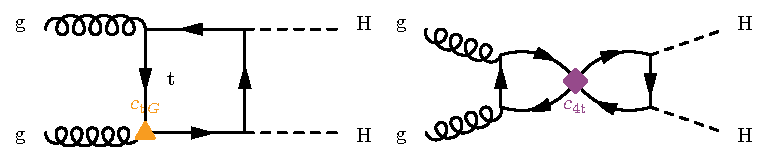
\includegraphics[width=\textwidth]{Diagrams/pdf/subleading}
    \caption{Representative Feynman diagrams induced by the subleading dimension-6 operators of Eq.~\eqref{eq:smeftL}~\cite{DiNoi:2024fdz}. Left: the chromomagnetic operator $c_{\PQt G}$ modifies the top--gluon vertex, marked by the triangle. Right: the four-fermion operators, collectively denoted $c_{4\PQt}$ and comprising $c_{Q\PQt}^{(1)}$, $c_{Q\PQt}^{(8)}$, $c_{QQ\PQt\PQt}$ and $c_{QQ}^{(8)}$, enter through the contact interaction between two top-quark loops, marked by the diamond.}
    \label{fig:feymnhh_subleading}
\end{figure}


\clearpage
\section{Parameterization of the differential cross section}
\label{sec:parameterization}

Due to the expensive MC generation, analytical descriptions of the total and differential cross sections are useful---if not mandatory---ways to explore the theory space, especially in the context of the heavy workflows used in experimental analyses. In SMEFT, the nonresonant \ggHH cross section can be parameterized as a function of the Wilson coefficients as follows:
%The event-level reweighting (ELR) technique consists of parameterizing the \HH cross section in terms of the coupling combinations appearing in the squared matrix element, and then defining weights that transport a given reference sample to any point of the EFT parameter space. The method was introduced for \HH production in Ref.~\cite{Carvalho:2017vnu} and developed to NLO QCD accuracy in Refs.~\cite{Alasfar:2023xpc,Cadamuro:2025car,ELR_R5}; here we only repeat what is needed to make this report self-contained and refer to Ref.~\cite{ELR_R5} for the derivation and for the validation of the technique.

%The differential \ggHH cross section at NLO QCD in SMEFT is written as a function of a phase-space variable (or set of variables) $\xi$ with bin index $j$. Denoting the leading Wilson coefficients by $c_{\text{H}},\,c_{\text{H}\mathrm{kin}},\,c_{u\PH},\,c_{\text{H}G}$ and the subleading ones by $c_{tG},\,c_{Qt1},\,c_{Qt8},\,c_{QQtt},\,c_{QQ8}$, the differential cross section can be organized as the SM term $A^j_0$ followed by two outer brackets: a ``leading only'' group containing the terms built solely from leading operators, and an ``include subleading'' group containing the terms with at least one subleading operator. Each outer group is in turn split into its linear and quadratic parts. The leading-only quadratic bracket collects every quadratic combination of the four leading operators in a single upper-triangular form $(c_{\text{leading}})\,Q\,(c_{\text{leading}})^{\!\top}$, with the squares on the diagonal and the distinct cross products above it. The quadratic-with-subleading bracket is written compactly as the bilinear form $(c_{\text{leading}})^{\!\top} M\,(c_{\text{subleading}})$, with the leading coefficients as rows and the subleading ones as columns:
\begin{equation}\label{eq:smeftpara_reorg}
\renewcommand{\arraystretch}{1.4}
\begin{split}
\frac{d}{d\xi_j}\sigma_{\ggHH}(\mathbf{c}^{\text{SMEFT}}_i) &= \\[6pt]
&\hspace{-2.2em} A^j_0
+ \underbrace{
\underbrace{
\begin{pmatrix} A^j_1 \\ A^j_2 \\ A^j_3 \\ A^j_4 \end{pmatrix}^{\!\!\top}
\begin{pmatrix} c_{\text{H}} \\ c_{\text{H}\mathrm{kin}} \\ c_{u\PH} \\ c_{\text{H}G} \end{pmatrix}
}_{\text{linear}}
+ \underbrace{
\begin{pmatrix} c_{\text{H}} & c_{\text{H}\mathrm{kin}} & c_{u\PH} & c_{\text{H}G} \end{pmatrix}
\begin{pmatrix}
A^j_5 & A^j_6 & A^j_7 & A^j_8 \\
0                 & A^j_9 & A^j_{10} & A^j_{11} \\
0                 & 0                 & A^j_{12} & A^j_{13} \\
0                 & 0                 & 0                    & A^j_{14}
\end{pmatrix}
\begin{pmatrix} c_{\text{H}} \\ c_{\text{H}\mathrm{kin}} \\ c_{u\PH} \\ c_{\text{H}G} \end{pmatrix}
}_{\text{quadratic}}
}_{\text{leading only}} \\[14pt]
&\hspace{-2.2em} + \underbrace{
\underbrace{
\begin{pmatrix} A^j_{15} \\ A^j_{16} \\ A^j_{17} \\ A^j_{18} \\ A^j_{19} \end{pmatrix}^{\!\!\top}
\begin{pmatrix} c_{tG} \\ c_{Qt1} \\ c_{Qt8} \\ c_{QQtt} \\ c_{QQ8} \end{pmatrix}
}_{\text{linear}}
+ \underbrace{
\begin{pmatrix} c_{\text{H}} & c_{\text{H}\mathrm{kin}} & c_{u\PH} & c_{\text{H}G} \end{pmatrix}
\begin{pmatrix}
A^j_{20} & A^j_{21} & A^j_{22} & A^j_{23} & A^j_{24} \\
A^j_{25} & A^j_{26} & A^j_{27} & A^j_{28} & A^j_{29} \\
A^j_{30} & A^j_{31} & A^j_{32} & A^j_{33} & A^j_{34} \\
A^j_{35} & A^j_{36} & A^j_{37} & A^j_{38} & A^j_{39}
\end{pmatrix}
\begin{pmatrix} c_{tG} \\ c_{Qt1} \\ c_{Qt8} \\ c_{QQtt} \\ c_{QQ8} \end{pmatrix}
}_{\text{quadratic}}
}_{\text{include subleading}}\\
&\hspace{-2.2em}=Poly(\mathbf{c}^{\text{SMEFT}}, \mathbf{A}^j),
\end{split}
\end{equation}
for $\xi$ a given phase-space variable, or variables in a multi differential description, and the corresponding bin $j$. The numeric $A$-coefficients carry the kinematic information of each of the squared-matrix element components.

The parameterization shown in Eq.~\eqref{eq:smeftpara_reorg} assumes the following options in \texttt{Powheg-Box-V2}: first, the quadratic truncation (option \texttt{b}); second, the $\textsc{includesubleading}==1$ option, to incorporate the subleading operators. This setup considers SM+linear dimension-6+quadratic dimension-6 contributions for leading operators at the cross section level, while subleading operators enter only linearly---therefore, $|\mathcal{M}_{\text{dim6}}^{\text{sublead}}|^2$ is neglected, and only interference terms with the leading part is considered. Double dimension-6 operator insertions ($\mathcal{M}_{\text{dim6}^2}$) are neglected in this truncation.

One advantage of using the analytical description in $Poly(\mathbf{c}^{\text{SMEFT}}, \mathbf{A}^j)$ is the flexibility in the choice of truncation. Once all coefficients are known, one can also describe cross sections in the linear truncation (option \texttt{a} in \texttt{Powheg} setup) by setting to zero the $A$'s contributing to the quadratic pieces. The mapping of the $A$-coefficients corresponding to leading-subleading operators and linear-quadratic truncations is shown in Table \ref{tab:smeft_matrix_blocks}. Additionally, one may notice that the definition of the combined Wilson coefficients $c_{\PH\mathrm{kin}}$ and $c_{QQ\PQt\PQt}$ of Sec.~\ref{sec:framework} not only reduces the parameter space dimension from 11 to 9, but also the number of required $A$-coefficients from 56 to 40, as a consequence. %The leading Wilson coefficients act on the same leading-order \ggHH diagrams as the HEFT couplings, which are drawn in Ref.~\cite{ELR_R5}; some of the diagrams specific to the subleading operators are shown in Fig.~\ref{fig:feymnhh_subleading}.

\begin{table}[h]
\centering
\renewcommand{\arraystretch}{1.3}
\begin{tabular}{lc}
\hline
Bracket & Coefficients \\
\hline
SM term                    &  $A^j_0$ \\
Linear, leading            & $A^j_1$--$A^j_4$ \\
Quadratic, leading only    &  $A^j_5$--$A^j_{14}$ \\
Linear, subleading         &  $A^j_{15}$--$A^j_{19}$ \\
Quadratic, with subleading & $A^j_{20}$--$A^j_{39}$ \\
\hline
\end{tabular}
\caption{Decomposition of the SMEFT parameterization of Eq.~\eqref{eq:smeftpara_reorg} into the SM term and four brackets, organized by truncation and by whether the operators involved are leading or subleading.}
\label{tab:smeft_matrix_blocks}
\end{table}

It is important to note, however, that this parameterization assumes no running of Wilson coefficients under RGEs. At NLO QCD, the anomalous dimension matrix mixes different Wilson coefficient contributions---except for $c_{\text{H}}$ and $c_{\text{Hkin}}$---, thereby making Eq.~\eqref{eq:smeftpara_reorg} invalid~\cite{Heinrich:2024rtg}. Notwithstanding, with some care a similar approach still possible when considering RGE effects, which is left for a future contribution.

Once the $A$-coefficients are known, one can apply the ELR approach in the same way as discussed in Ref.~\cite{ELR_R5}:
\begin{equation}\label{eq:reweightformula}
w(\mathbf{c}^{\text{SMEFT}}_i)=\frac{Poly(\mathbf{c}^{\text{SMEFT}}_i, \mathbf{A}^j)}{Poly(\mathbf{c}_{\text{ref}}, \mathbf{A}^j)}w(\mathbf{c}_{\text{ref}})\;,
\end{equation}
where $\mathbf{c}_{\text{ref}}$ denotes a reference sample that is reweighted to any point fixed by $\mathbf{c}^{\text{SMEFT}}_i$ in SMEFT parameter space, and $w(\mathbf{c}_{\text{ref}})$ the corresponding generator-level weight.

%Furthermore, $c_{QQ}^{(1)}$ and $c_{\PQt\PQt}$ are combined into a single parameter $c_{QQ\PQt\PQt}=c_{QQ}^{(1)}+c_{\PQt\PQt}$, as their contributions to the amplitude can be factorized CITE. In addition, we are using the common convention for the kinetic coefficients $c_{Hkin}=c_{\PH\Box}-\frac{1}{4}c_{\PH D}$. These simplifications reduce the number of parameters from 11 to 9, which allows us to parameterize the cross section in terms of 40 $A-$coefficients in equation \eqref{eq:smeftpara_reorg}, rather than 56. The effect of the leading Wilson coefficients on the leading order \ggHH Feynman diagrams is indicated in Figure~\ref{fig:feymnhh}. 
%The 40 coefficients $A^j_k$ are numbered in ascending order following the reading order of the matrices (left to right, top to bottom, skipping the zero entries of $Q$). In the leading-only bracket the matrix $Q$ holds the squares of the leading operators on its diagonal and their distinct pairwise products above it, while the with-subleading bracket collects the remaining quadratic combinations in the matrix $M$. Table~\ref{tab:smeft_matrix_blocks} summarizes the content of the brackets.




%Once the $A$-coefficients are known, the differential cross section at any point of the parameter space follows from the analytical formula, and any reference sample can be reweighted event by event through the ratio
%\begin{equation}\label{eq:reweightformula}
%w(\mathbf{c}^{\text{SMEFT}}_i)=\frac{Poly(\mathbf{c}^{\text{SMEFT}}_i, \mathbf{A}^j)}{Poly(\mathbf{c}_{\text{ref}}, \mathbf{A}^j)}w(\mathbf{c}_{\text{ref}})\;,
%\end{equation}
%which allows any phase-space variable $\Omega$ to be built, not only those used to extract the formula.

\clearpage
\section{Event generation and fit to the $A$-coefficients}
\label{sec:eventsimulation}

\subsection{Simulation setup}



In order to fit the $A$-coefficients, events are generated with the \texttt{ggHH\_SMEFT} implementation of \texttt{Powhex-Box-V2}~\cite{powheg1,powheg2,powheg3,Heinrich:2023rsd}. A grid of 4500 SMEFT points is considered at $\sqrt{s}=13.6$ TeV. The grid is built in two pieces: first, with 2D scans between the Wilson coefficients; second, considering mutual variations of Wilson coefficients in two multi-dimensional Gaussians (one varying $c_\PH,\,c_{\PH \mathrm{kin}},\,c_{u\PH},\,c_{\PH G},\,c_{\PQt G}$, and the other varying all nine parameters) centered on the SM point. The considered ranges are shown on Table \ref{tab:SMEFTcouplings}, where the region covered takes into consideration the global fit constrains described in Refs.~\cite{SMEFiT:2021, Celada:2024mcf}, but with enlarged bounds in order to ensure coverage to regions accessed by searches with less sensitivity. The samples were generated with 50000 events each, using the PDF set \texttt{PDF4LHC15nlo30}\cite{pdf}. The top-quark mass is set to $m_\PQt=173.0$~GeV and is renormalized in the on-shell scheme, while the Higgs boson mass is set to $m_\PH=125.0$~GeV. The renormalization and factorization scales are set to $\mu_R=\mu_F=\mHH/2$. The strong coupling constant $\alpha_s(m_\PZ)=0.118$ is taken from the PDF set and the Wilson coefficients are given at $\Lambda=1$~TeV. The RGE running of the Wilson coefficients is kept switched off in \texttt{Powheg}.




\begin{table}[h!]
\centering
\renewcommand{\arraystretch}{1.2}
\begin{tabular}{c c c c}
\hline
2D scans & 5D Gaussian & 9D Gaussian & Total \\
\hline
$1632$ & $1700$ & $1168$ & $4500$ \\
\end{tabular}
\caption{Grid composition: pairwise two-dimensional scans and multi-dimensional Gaussian centered on the SM. 
}
\label{tab:grids_comp}
\end{table}
\begin{table}[h!]
\centering
\small
\begin{tabular}{|c|c|c|}
\hline
Parameter & Range & SMEFiT name \\
\hline
$c_{\PH}$              & $[\,-50, 50\,]$           & --- \\
$c_{\PH \mathrm{kin}}$ & $[\,-8, 8\,]$               & $c_{\varphi\Box}$, $c_{\varphi D}$ \\
$c_{u\PH}$          & $[\,-10, 7\,]$              & $c_{t\varphi}$ \\
$c_{\PH G}$            & $[\,-0.1, 0.03\,]$     & $c_{\varphi G}$ \\
$c_{\PQt G}$           & $[\,-0.3, 1.0\,]$      & $c_{tG}$ \\
$c_{Q\PQt}^{(1)}$      & $[\,-20, 20\,]$            & $c^{1}_{Qt}$ \\
$c_{Q\PQt}^{(8)}$      & $[\,-20, 20\,]$           & $c^{8}_{Qt}$ \\
$c_{QQ\PQt\PQt}$       & $[\,-20, 20\,]$           & $c^{1}_{QQ}+c^{1}_{tt}$ \\
$c_{QQ}^{(8)}$         & $[\,-20, 20\,]$           & $c^{8}_{QQ}$ \\
%$c_{\PH}$              & $[\,-50, 50\,]$ \\
%$c_{\PH \mathrm{kin}}$ & $[\,-8, 8\,]$ \\
%$c_{u\PH}$          & $[\,-10, 7\,]$ \\
%$c_{\PH G}$            & $[\,-0.1, 0.03\,]$ \\
%$c_{\PQt G}$           & $[\,-0.3, 1.0\,]$ \\
%$c_{Q\PQt}^{(1)}$      & $[\,-20, 20\,]$ \\
%$c_{Q\PQt}^{(8)}$      & $[\,-20, 20\,]$ \\
%$c_{QQ\PQt\PQt}$       & $[\,-20, 20\,]$ \\
%$c_{QQ}^{(8)}$         & $[\,-20, 20\,]$ \\
\hline
\end{tabular}
\caption{Ranges of the Wilson coefficients assumed to derive the $A$-coefficients. The correspondence with SMEFiT \cite{Giani:2023gfq} names is shown in the last column. We use as reference the $95\%$~CI marginalized bounds at $\mathcal{O}(\Lambda^{-4})$ in Refs.~\cite{SMEFiT:2021, Celada:2024mcf}, but with enlarged bounds.}
\label{tab:SMEFTcouplings}
\end{table}
%\begin{table}[h!]
%\centering
%\begin{tabular}{c|c}
%\hline
%Input & Value  \\
%\hline
%Generator          & \texttt{Powheg-Box-V2} at NLO QCD \\
%$m_t$              & $173.0$ GeV \\
%$m_\text{H}$              & $125.0$ GeV \\
%$\mu_{R}=\mu_F$ & $m_{\text{HH}}/2$  \\
%PDF & \texttt{PDF4LHC15\_nlo\_30\_pdfas} \\
%PDF ($100$ TeV)    & \texttt{PDF4LHC21\_40\_pdfas} \\
%$\alpha_s(m_Z)$    & $0.118$ \\
%$\sqrt{s}$         & $13.6$ TeV \\
%$\Lambda$          & $1$ TeV \\
%\hline
%\end{tabular}
%\caption{\texttt{Powheg} input parameters. The top-quark mass is renormalized in the on-shell scheme and the $\alpha_s$ value is taken from the corresponding PDF set. The renormalization and factorization scales are set to $m_{\text{HH}}/2$, and the new physics scale is set to $\Lambda=1$ TeV.}
%\label{tab:POWHEGinput}
%\end{table}

\subsection{Derivation of the coefficients}
\label{sec:a-coeff-derivation}
%\subsubsection{Coefficients at $\sqrt{s}=13.6$ TeV}
The strategy for extracting the $A$-coefficients at $\sqrt{s}=13.6$ TeV follows Ref.~\cite{ELR_R5}, to which we refer for the full discussion of the choice of reweighting variables and of the fitting algorithm. The latter relies in a per bin iteratively reweighted least squares (IRLS) fit, which takes as input all the generated points described in the previous Section. Table \ref{tab:binedge} displays the considered binning, where the 1D-$m_{\HH}$ description in the high-mass region ($m_\HH>1000$ GeV) is needed for ensuring statistical stability. 


\renewcommand{\arraystretch}{1.1}
\begin{table}[t]
\centering
\begin{tabular}{|c|l|}
\hline
Variable & Bin edges \\ \hline
%\multicolumn{2}{|c|}{\textbf{3D}} \\ \hline
$m_{\HH}\:\text{[GeV]}$
& \textcolor{blue}{$250,\:270,\:290,\:310,\:330,\:350,\:370,\:390,\:410,\:430,\:450,\:470,\:490$} \\
& \textcolor{blue}{$510,\:530,\:550,\:570,\:590,\:610,\:630,\:650,\:670,\:690,\:710,\:730,\:750$} \\
& \textcolor{blue}{$800,\:850,\:900,\:950,\:1000$}$,\:1050,\:1100,\:1200,\:1300,\:1400,\:1500,$\\
& $1600,\:1800,\:2000,\:13600$ \\ \hline
$|\cos\theta^*|$
& \textcolor{blue}{$0.0,\:0.25,\:0.5,\:0.75,\:1.0$} \\ \hline
$p^{\HH}_T\:\text{[GeV]}$
& \textcolor{blue}{$0.0,\:20,\:40,\:60,\:80,\:100,\:140,\:200,\:290,\:2500$} \\ \hline
\end{tabular}
\caption{Bin edges considered. The blue color indicates where binning is 3D. The high-mass region ($m_{\text{HH}}>1000$ GeV) it is always one-dimensional due to the lack of statistics.}
\label{tab:binedge}
\end{table}
\renewcommand{\arraystretch}{1.0}
\begin{figure}[h!]
  \centering
  % First group: 2 x 2
  \begin{minipage}[b]{0.495\linewidth}
    \centering
    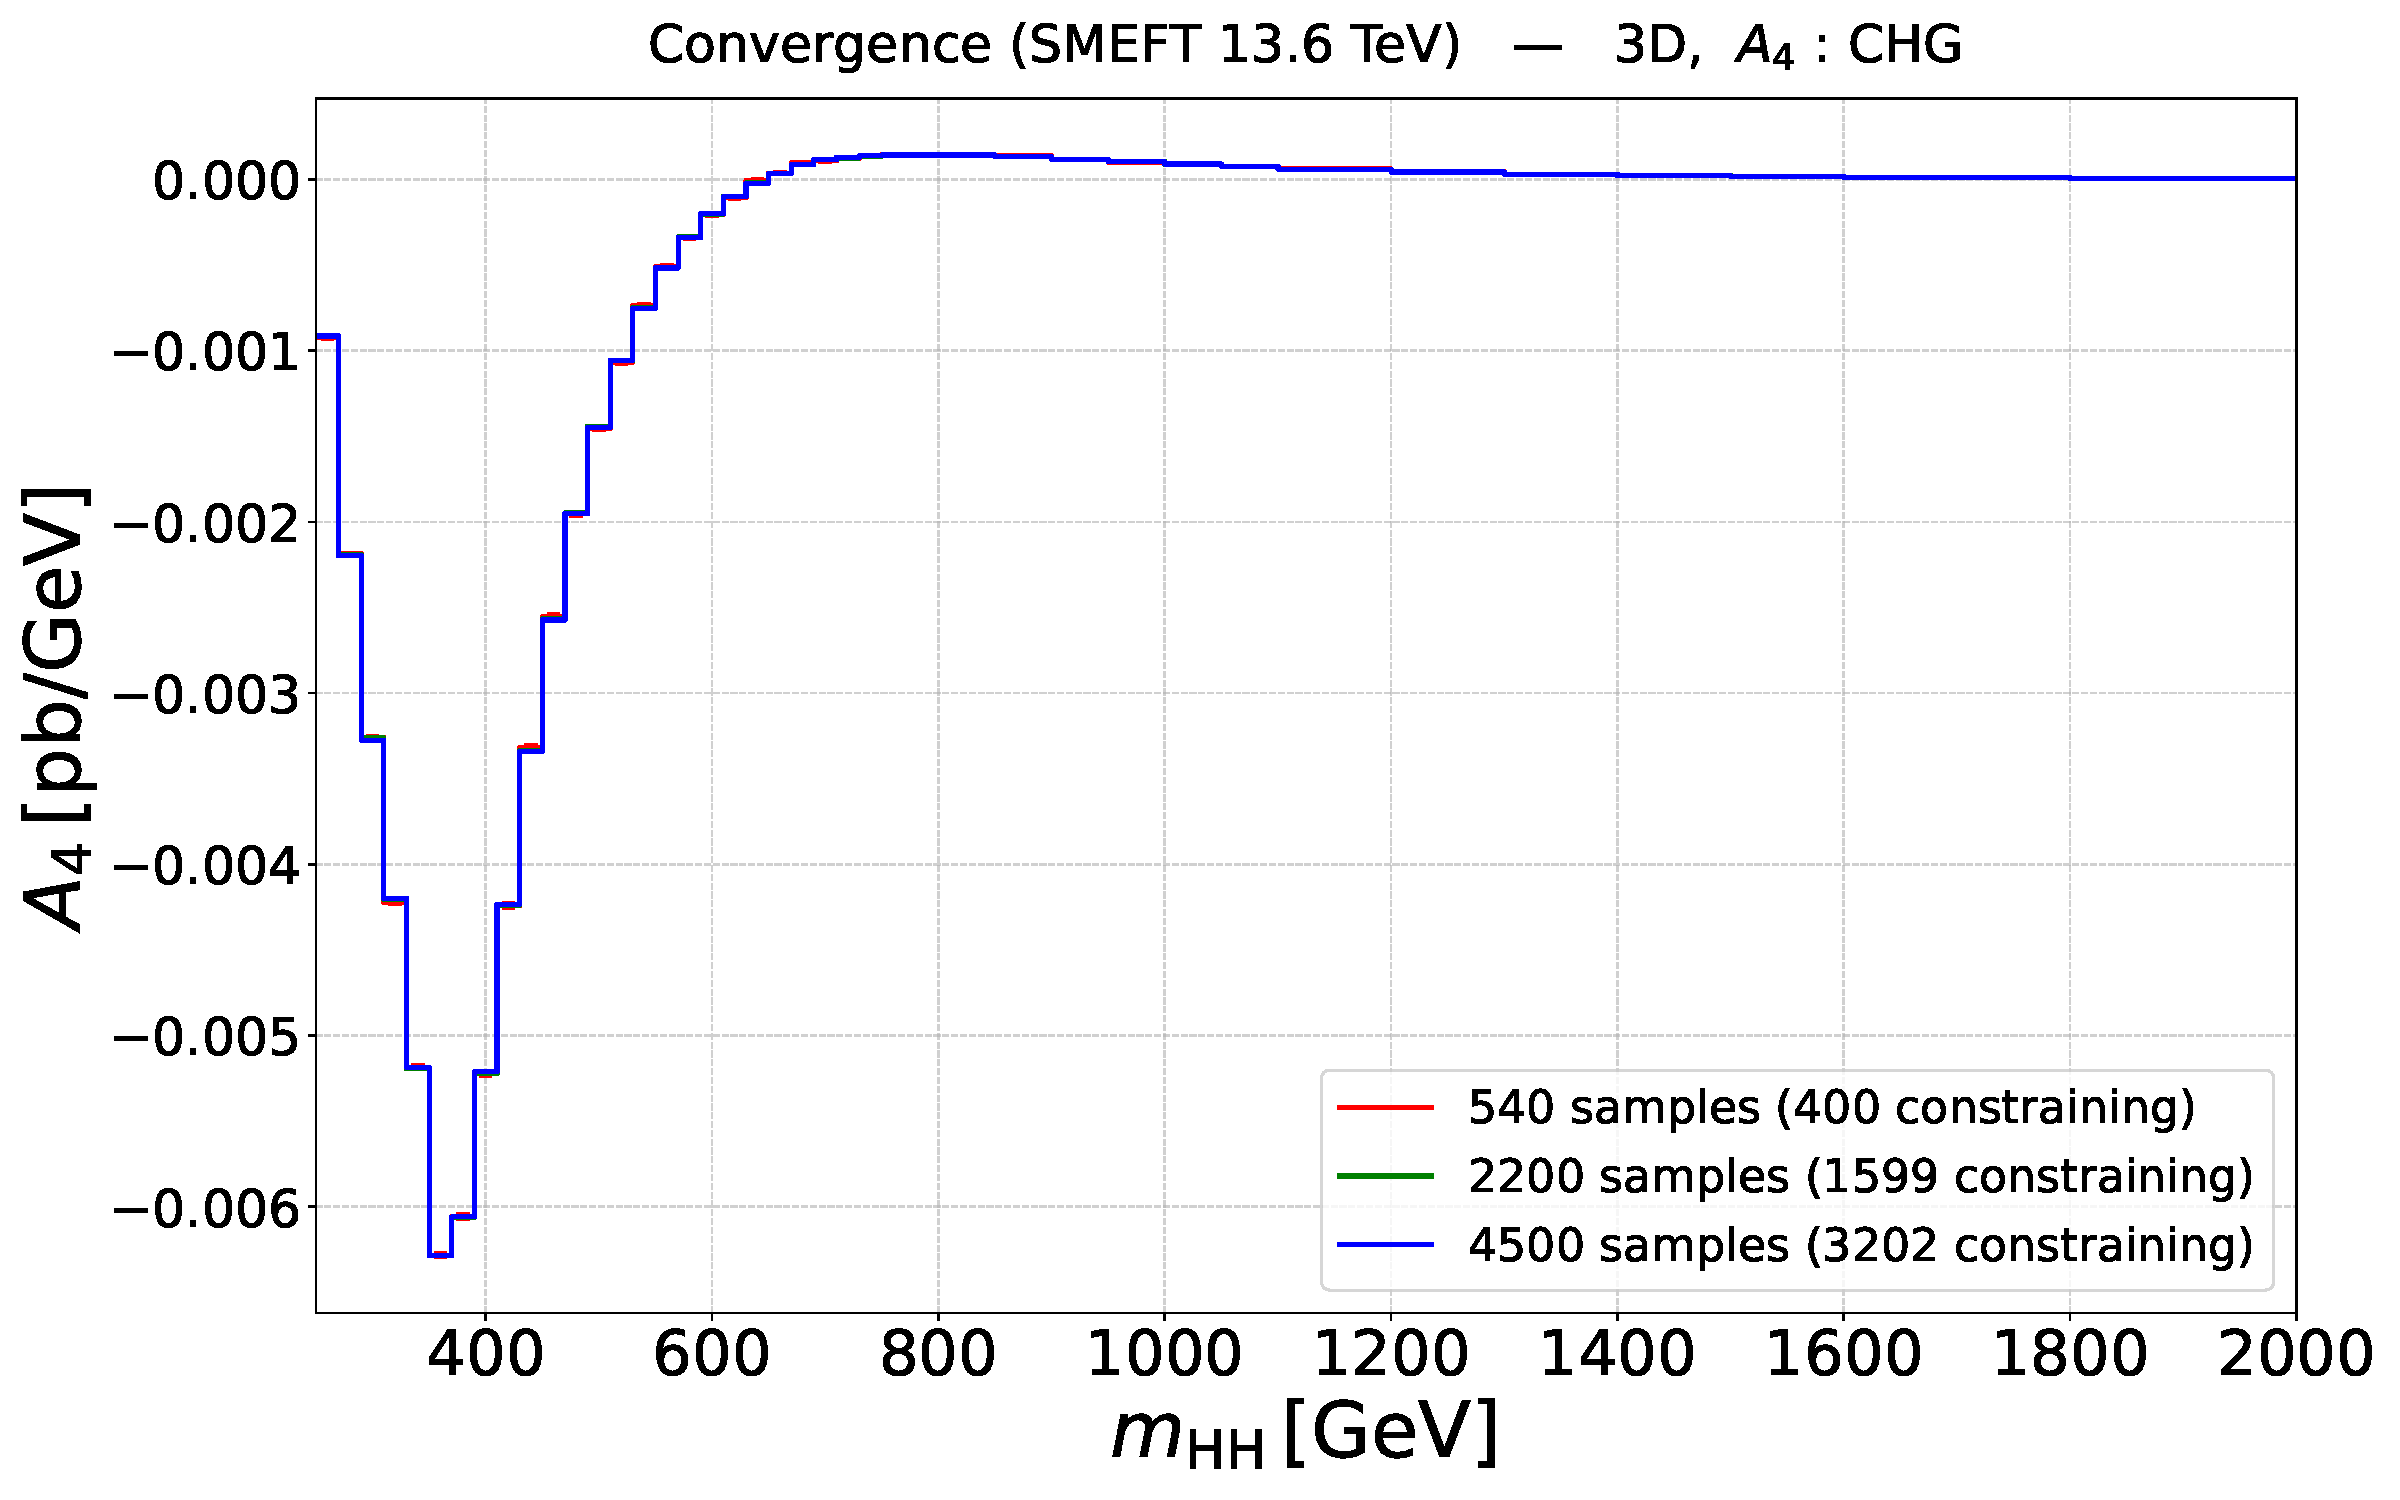
\includegraphics[width=\linewidth]{plots/plot_param4_250_2000_3d_convergence_9D.pdf}
  \end{minipage}
  \hfill
  \begin{minipage}[b]{0.495\linewidth}
    \centering
    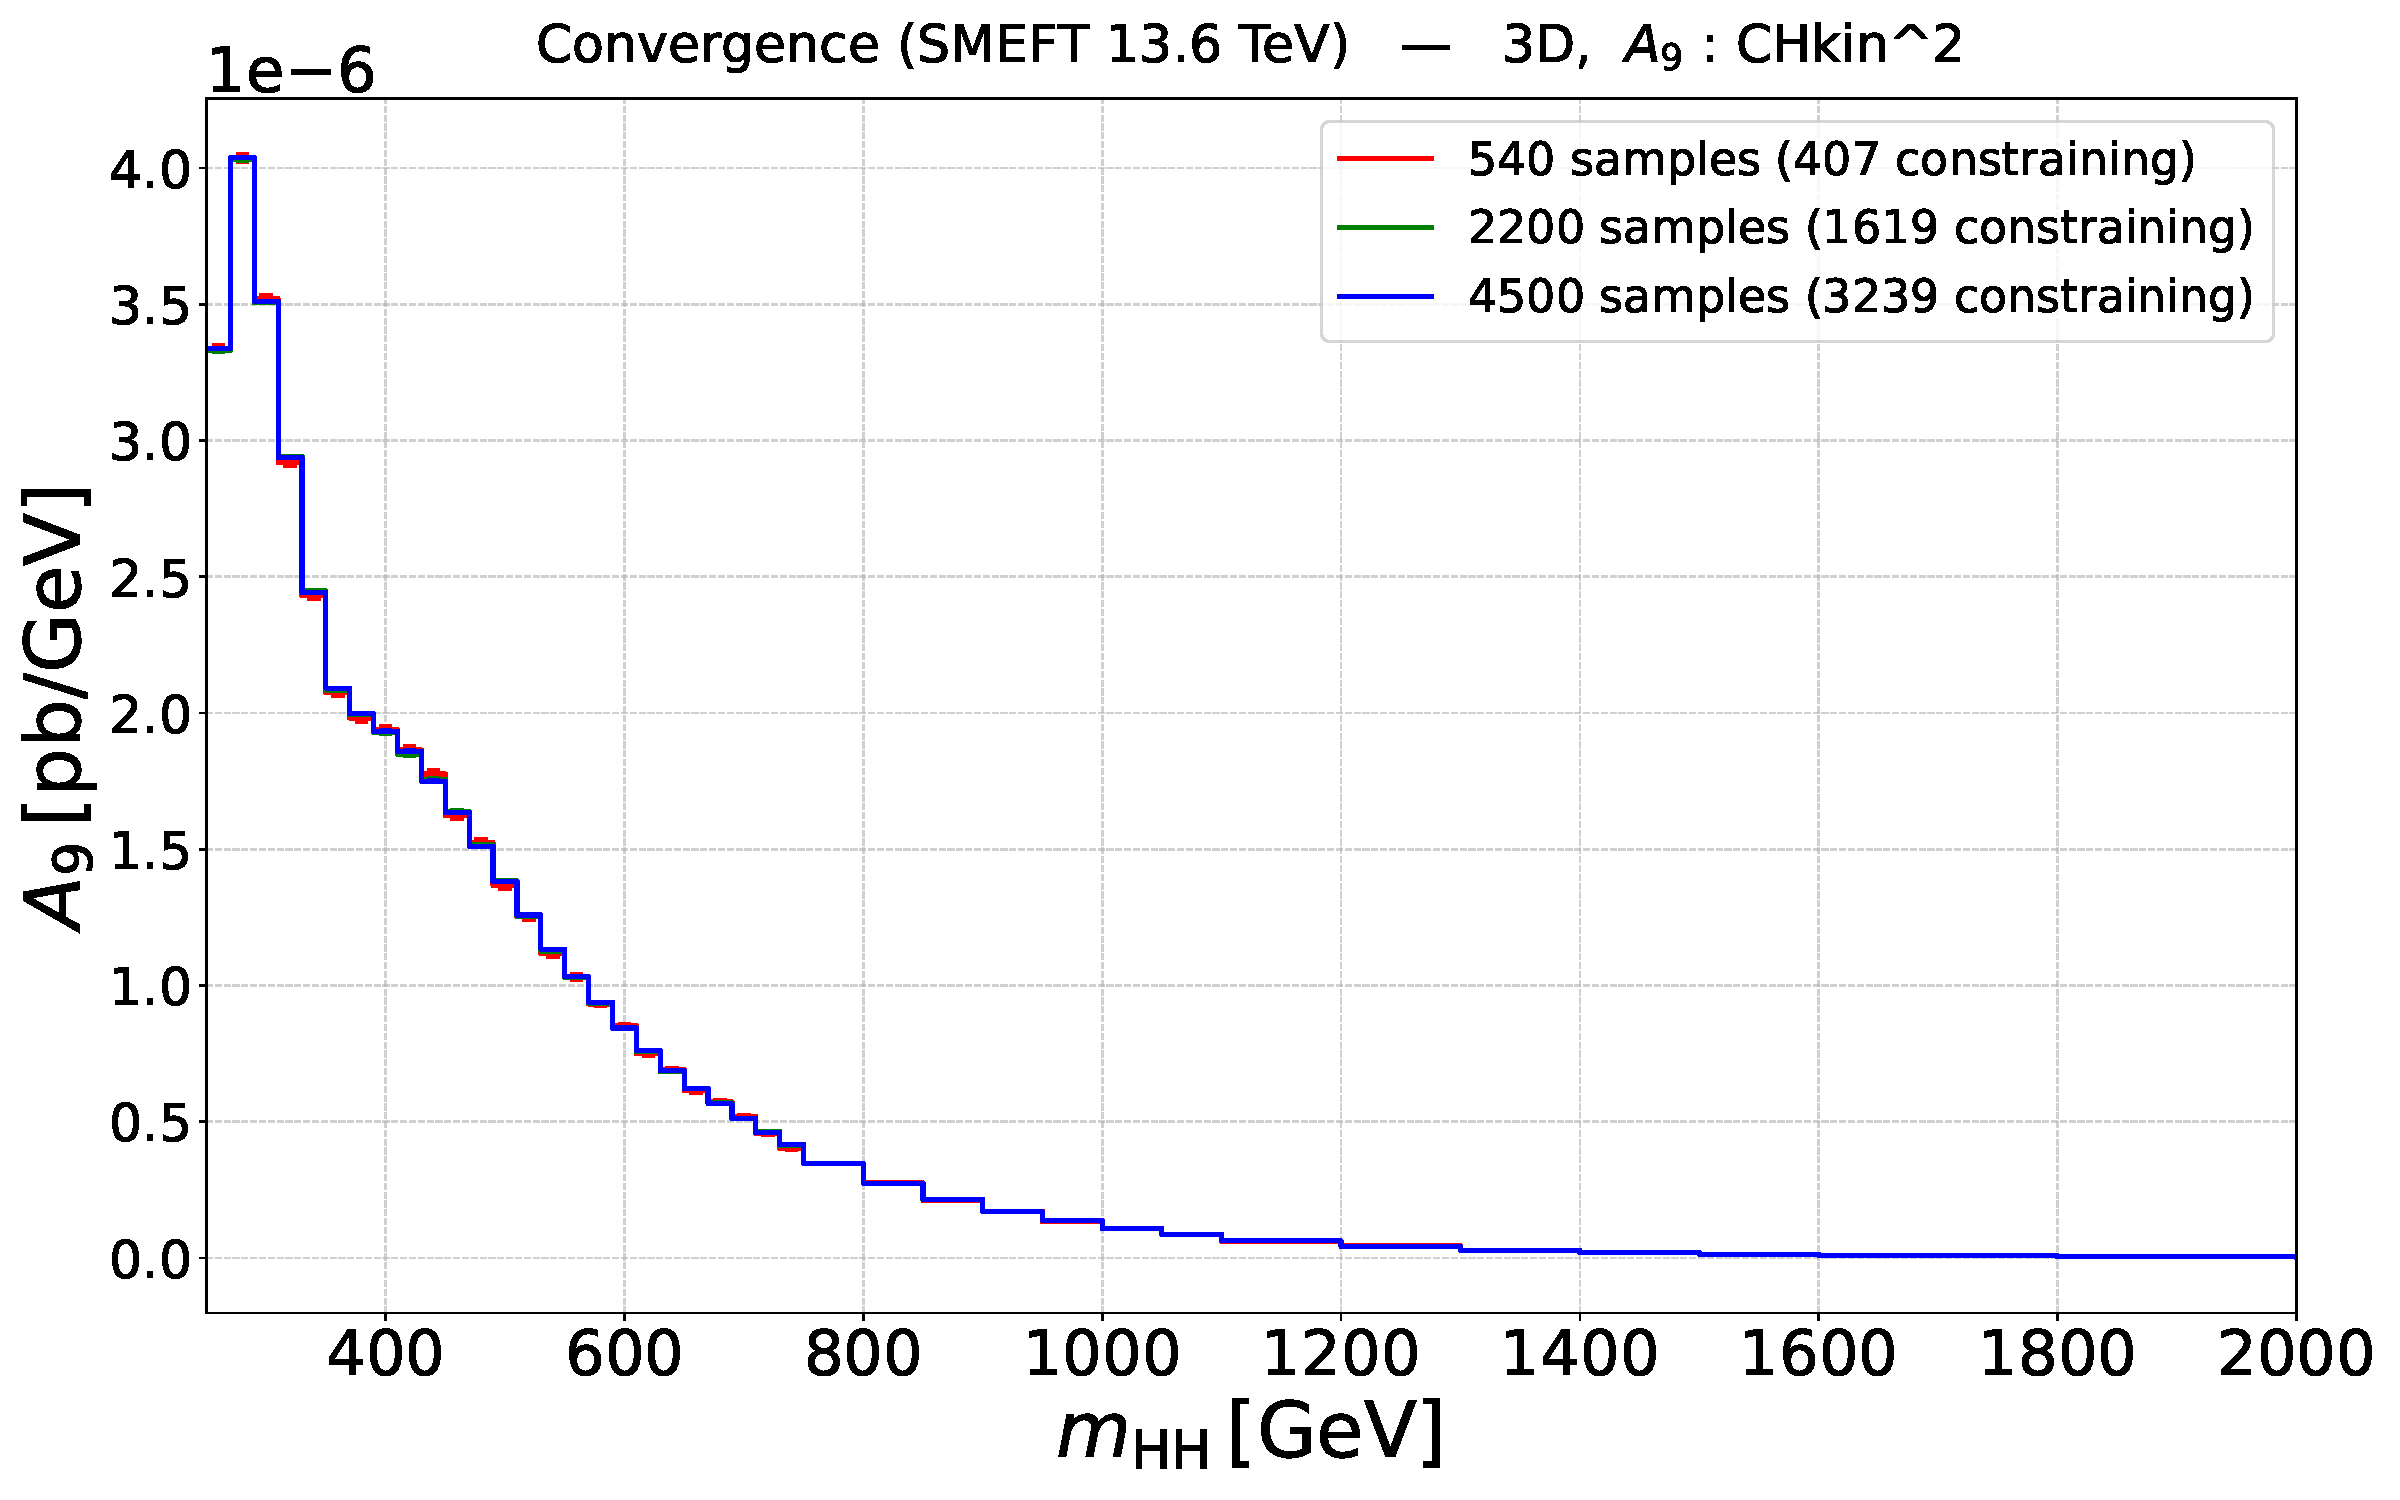
\includegraphics[width=\linewidth]{plots/plot_param9_250_2000_3d_convergence_9D.pdf}
  \end{minipage}
  \vspace{0.5em}
  \begin{minipage}[b]{0.495\linewidth}
    \centering
    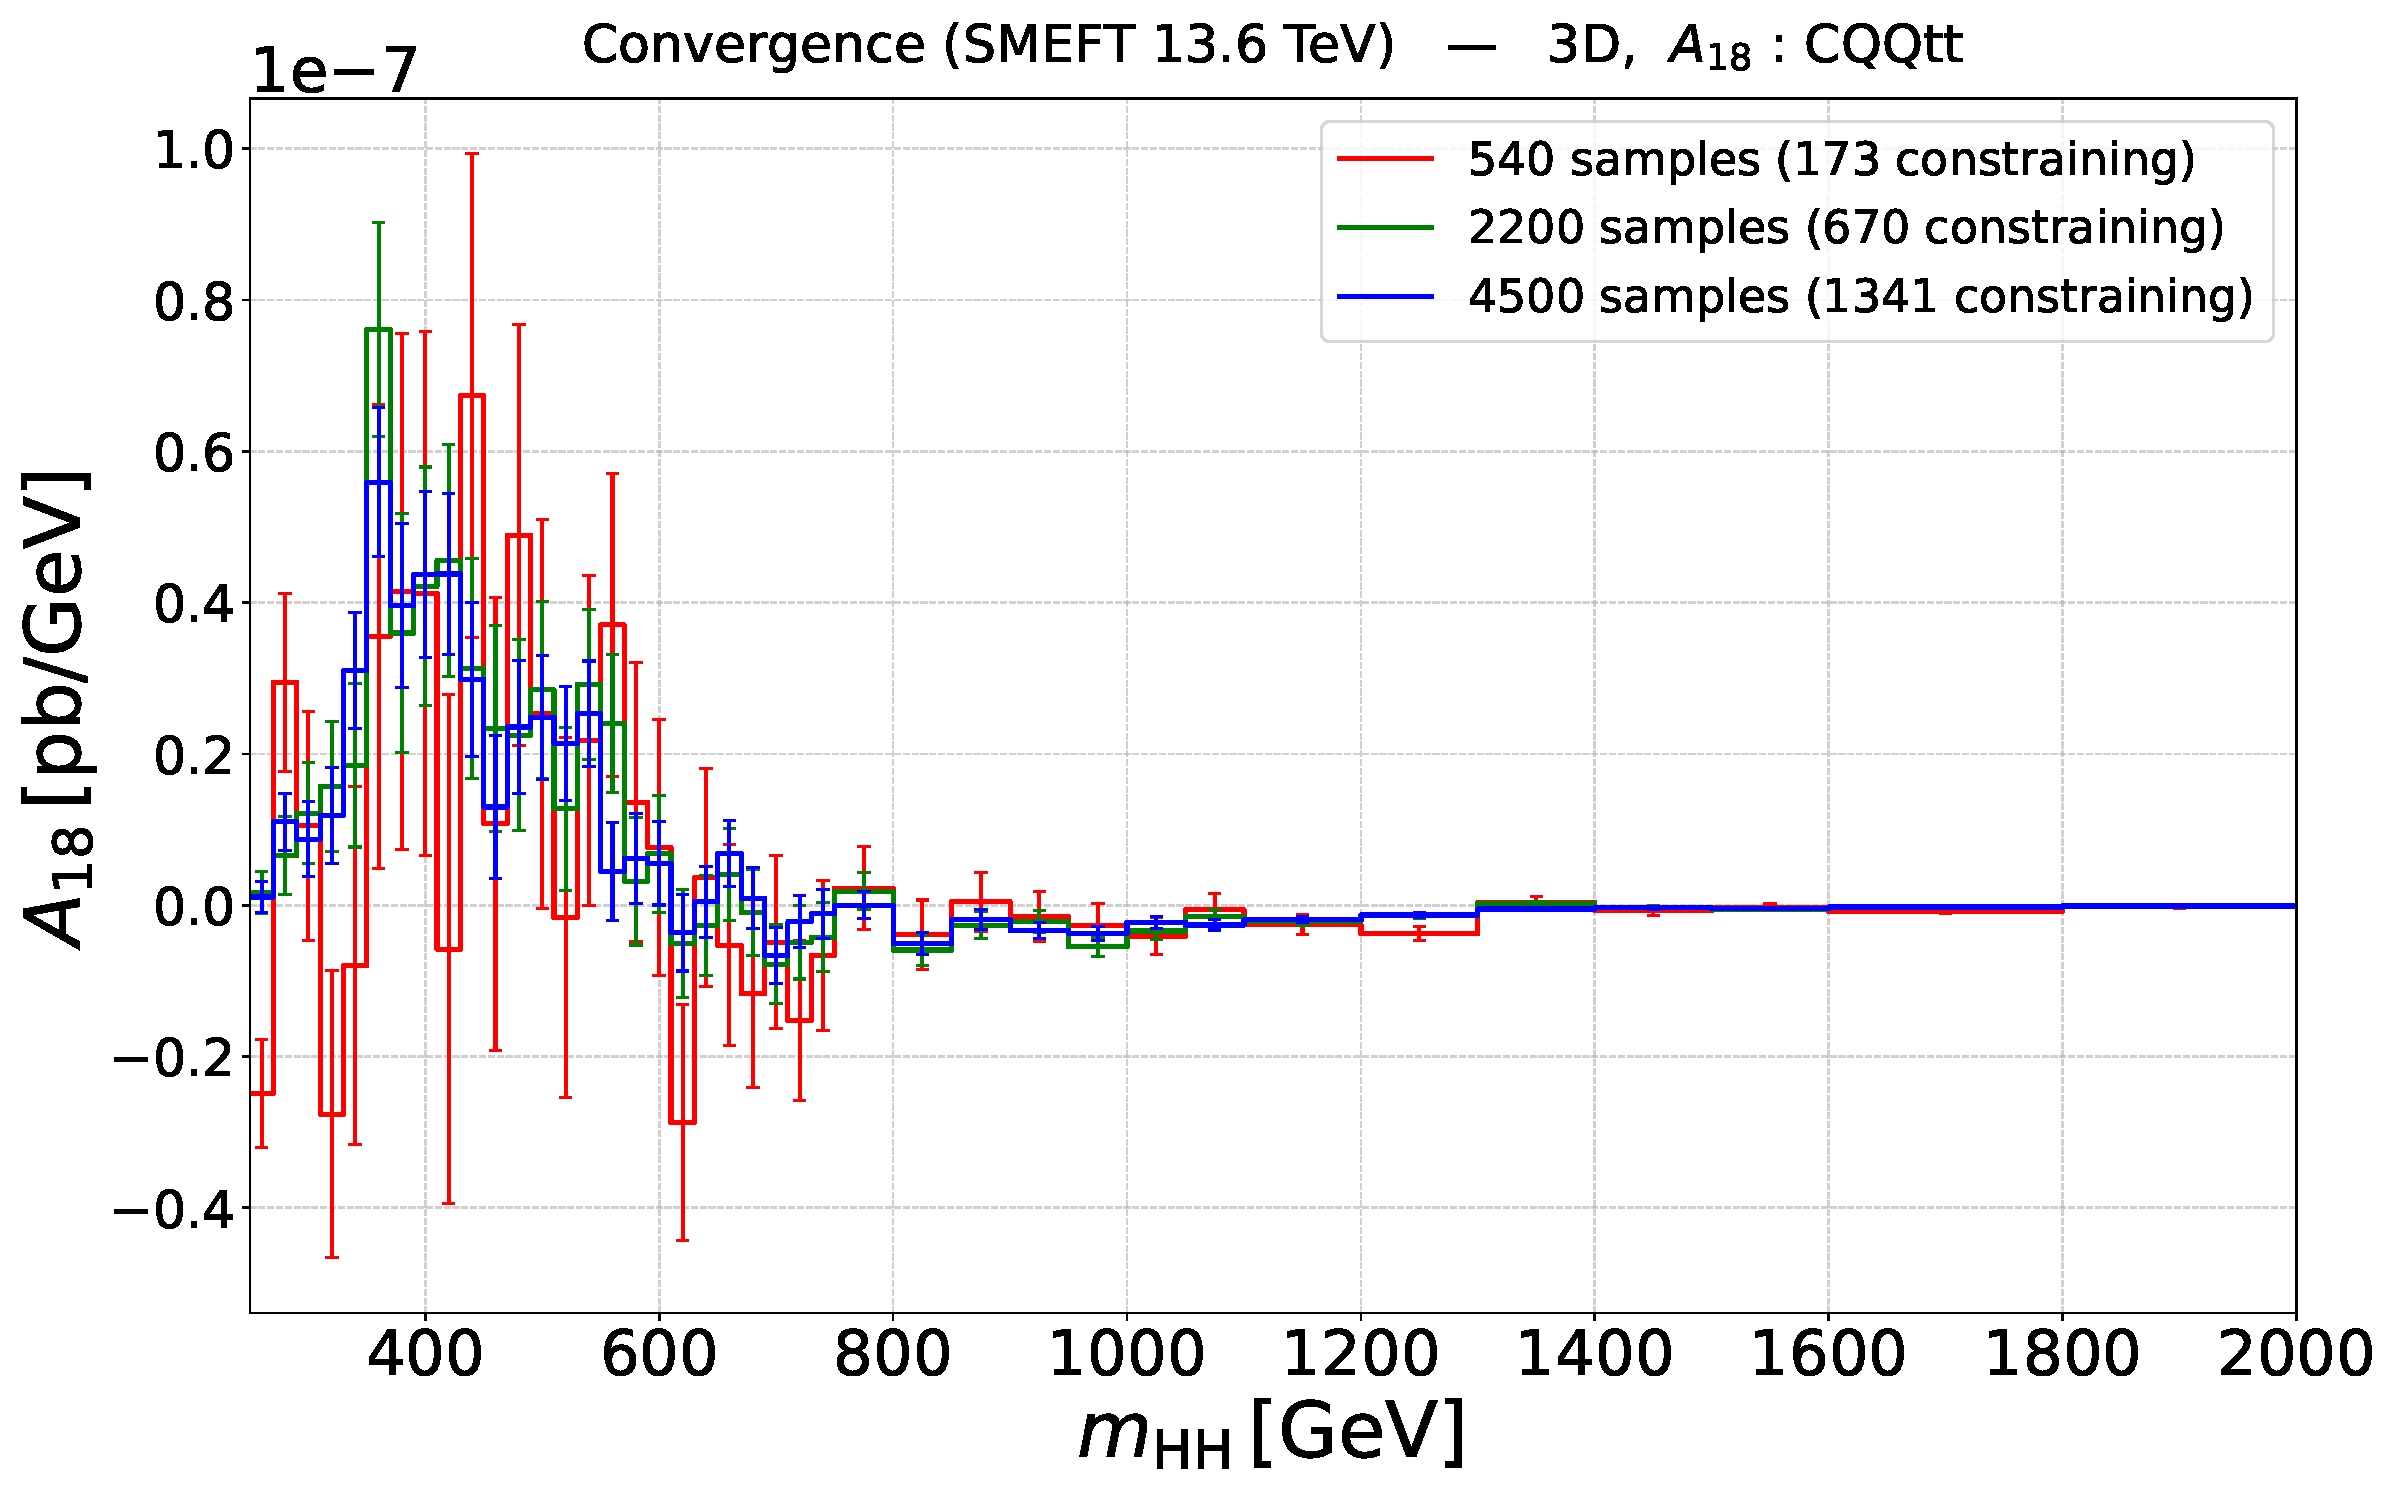
\includegraphics[width=\linewidth]{plots/plot_param18_250_2000_3d_convergence_9D.pdf}
  \end{minipage}
  \hfill
  \begin{minipage}[b]{0.495\linewidth}
    \centering
    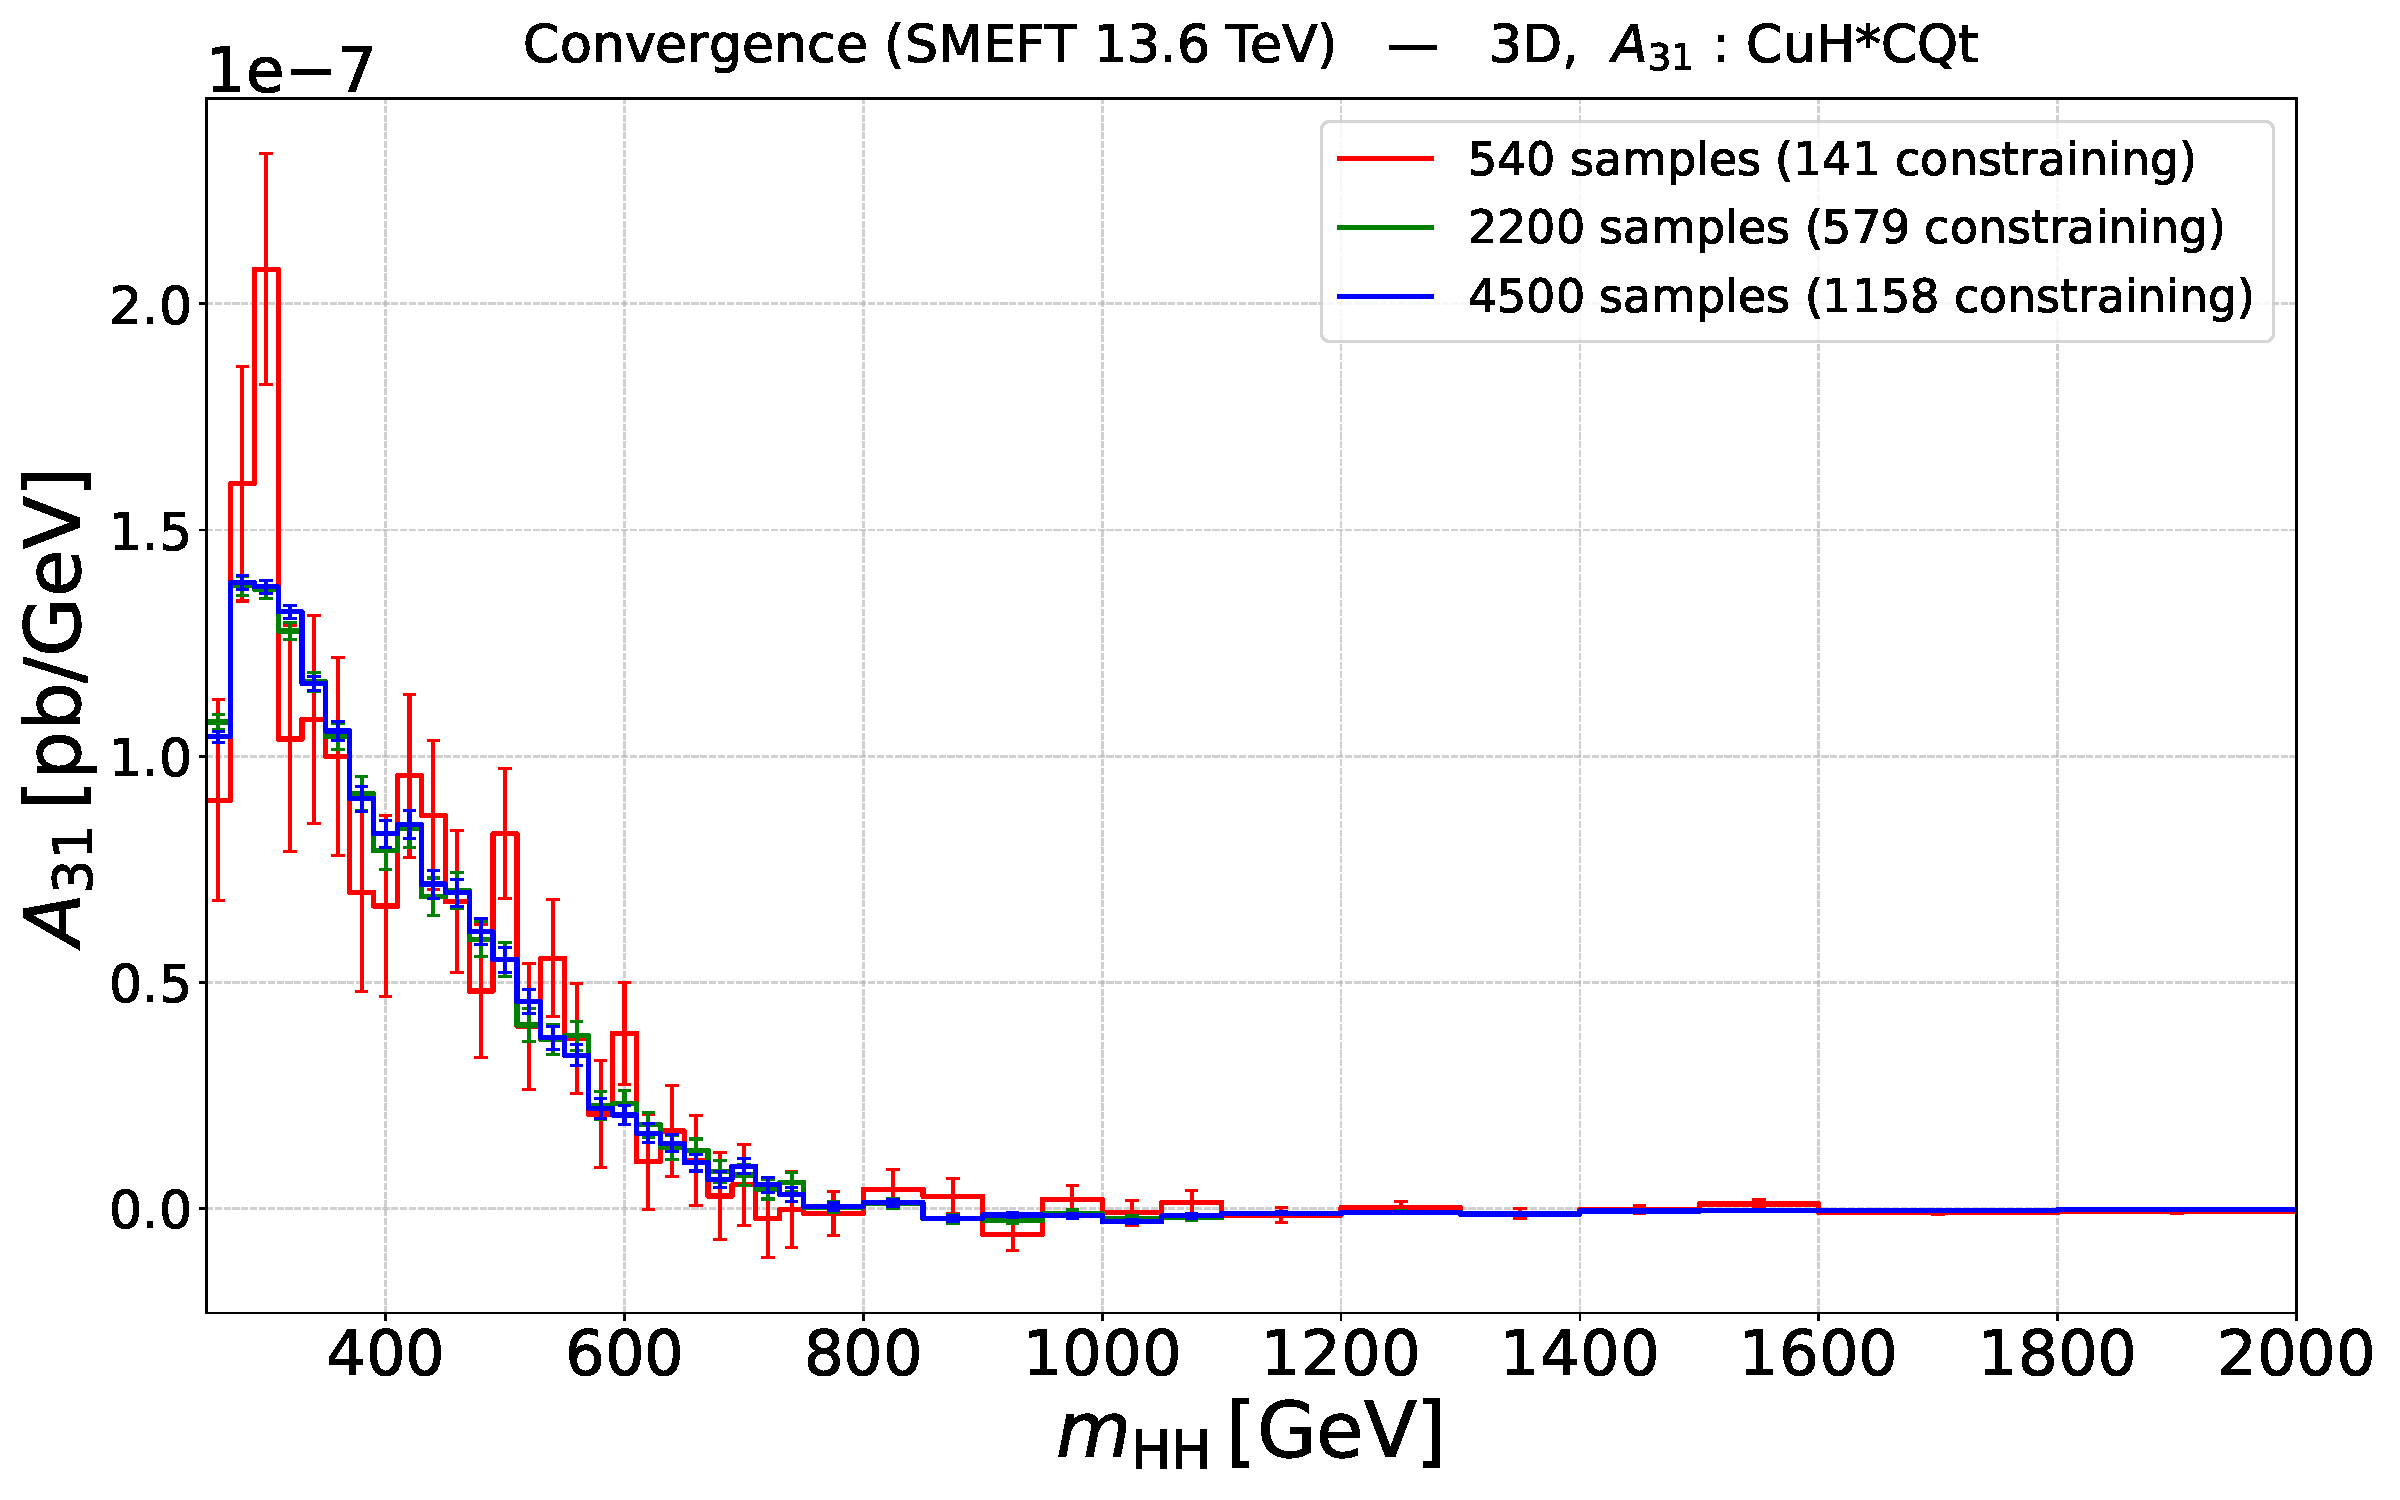
\includegraphics[width=\linewidth]{plots/plot_param31_250_2000_3d_convergence_9D.pdf}
  \end{minipage}
  \caption{Convergence of the 3D $A$-coefficients projected into $m_{\text{HH}}$. The upper panel shows coefficients arising from leading-operator terms, while the lower panel shows coefficients arising from subleading and leading$\times$subleading terms.}
  \label{fig:convergence}
\end{figure}

The convergence of some of the coefficients is exhibited in Fig.~\ref{fig:convergence}. All coefficients stemming from leading-only operator insertions show quick convergence, as represented by the upper panel. On the other hand, all coefficients involving subleading components require more samples to stabilize, regardless coming from linear (bottom-left) or quadratic (bottom-right) contributions.

The final set of coefficients consistent with the updated PDF set (\texttt{PDF4LHC21\_40} \cite{PDF4LHC21}) and at all COM energies $\sqrt{s}=13$,  $13.6$, $14$ TeV, are obtained with the transport technique discussed in Ref.~\cite{ELR_R5}, and the validation of this procedure in SMEFT is shown in Appendix ~\ref{sec:validation_transport}. All set of coefficients and the corresponding covariance matrices are available as supplementary files in the arXiv submission.


%\subsubsection{Coefficients at $\sqrt{s}=13$ and $14$ TeV}
%The coefficients at $\sqrt{s}=13$ and $14$ TeV can be derived from the $13.6$ TeV ones by applying transfer factors that account for the effects of the PDFs at different COM energies. For a given generated event, the subprocess final state kinematics (e.g. $\{m_{\HH},|\cos\theta^*|,p^\HH_T|$) are fixed. Therefore, with $\hat{s}=x_1x_2s$ and $y=\frac{1}{2}\ln{(x_1/x_2)}$ held constant, a change in the COM energy implies in scaling the momentum fractions with $x^\prime_i=x_i\sqrt{s/s^\prime}$ and can be factorized as
%\begin{equation}\label{eq:transport}
%    \frac{d\sigma(\sqrt{s}^\prime)/d\hat{s}dy}{d\sigma(\sqrt{s})/d\hat{s}dy}=\frac{s}{s^\prime}\frac{f(x^\prime_1,\mu_F)f(x^\prime_2,\mu_F)}{f(x_1,\mu_F)f(x_2,\mu_F)},
%\end{equation}
%which depends only on initial state quantities. From the parameterization shown in Eq.~\eqref{eq:smeftpara_reorg}, this is to say that the $A$-coefficients can be scaled with per bin transfer factors that multiplies all the 40 terms:
%\begin{equation}
%    A^i_j(\sqrt{s}=13,14\text{ TeV})=T_jA^i_j(\sqrt{s}=13.6 \text{ TeV}).
%\end{equation}
%These factors can be extracted by accessing the initial state partons in the generated events at $\sqrt{s}=13.6$ TeV, to which one can use the $x\to x^\prime$ transport to get both the numerator and denominator in Eq.~\eqref{eq:transport}. Once this is computed for all events, the per bin $T$-factors are then extracted and used to rescale the $A$-coefficients to both $13$ and $14$ TeV. For a given bin $j$, the covariance matrices are accordingly scaled as
%\begin{equation}
%C_{kl}(\sqrt{s}',j) = T_j^2 \left[ C_{kl}(\sqrt{s},j)
%                      + r_j^2\, A_k^j A_l^j \right],
%\label{eq:energy_cov}
%\end{equation}
%since $cov(TA_k,TA_l)=T^2cov(A_k,A_j)$. The second term is due to the statistical uncertainty $r_j$ in the extraction of the $T_j$-factor.


%The new coefficients are validated with additional samples generated at the corresponding COM energies and found to provide the same level of accuracy as the fitted coefficients in $13.6$ TeV, but without requiring the generation of thousand of new samples for new dedicated fits. Additional details and validation of this procedure is provided in Appendix~\ref{sec:validation_transport}.    

%The 3D coefficients at all three energies, together with their covariance matrices, are available as ancillary files in the arXiv submission.


%\subsection{Linear and quadratic truncations}

%The coefficients are also validated against benchmark points generated separately in the linear and in the quadratic truncation, which is the subject of Sec.~\ref{sec:truncation}.

%\newpage
%\subsection{Renormalization-group running of the Wilson coefficients}
%The RGE running of the Wilson coefficients is kept \emph{switched off} in
%\texttt{Powheg}, and the coefficients are taken at the fixed scale $\Lambda=1$~TeV
%throughout. This is a deliberate choice, not a simplification of convenience.
%With running enabled the coefficients entering the matrix element become
%$c_i(\mu_{\text{EFT}})$ evaluated at the dynamical scale $\mu_{\text{EFT}}=\mHH/2$,
%so every generated event carries a different effective set of couplings. The
%$A$-coefficients of Eq.~\eqref{eq:smeftpara_reorg} would then no longer be pure
%numbers attached to the process: they would absorb the running, become specific to
%one choice of $\Lambda$ and one running implementation, and lose the property that
%makes the parameterization useful in the first place --- that a user can evaluate
%the same polynomial at any coefficient point without regenerating anything. Since
%$\mu_{\text{EFT}}$ is tied to \mHH, the effect does not even factorize between the
%inclusive and the differential parameterizations.

%The effects themselves are not negligible at the precision these templates aim
%for, and are becoming a standard part of SMEFT
%interpretations~\cite{Maltoni:2024dpn,terHoeve:2025rge}. They are, however,
%recoverable after the fact, and this is worth stating explicitly because it is the
%reason the choice above costs nothing. At leading logarithmic accuracy the
%solution of the dimension-6 RGEs is \emph{linear} in the Wilson coefficients,
%\begin{equation}
%c_i(\mu) = U_{ij}(\mu,\Lambda)\,c_j(\Lambda),
%\qquad
%U_{ij}(\mu,\Lambda) = \delta_{ij} + \frac{\gamma_{ij}}{16\pi^2}\ln\frac{\mu}{\Lambda}
%+ \mathcal{O}(\ln^2) ,
%\label{eq:rge_linear}
%\end{equation}
%with $\gamma_{ij}$ the anomalous-dimension matrix. A linear map composed with a
%quadratic polynomial is again a quadratic polynomial, so the templates extracted
%with running off can be used to obtain the running result simply by evaluating
%them at the transformed coefficient vector $U(\mu,\Lambda)\,c(\Lambda)$, with
%$U$ obtained from any of the standard solvers. Two conditions apply. First, the
%transformation must be done \emph{differentially}, bin by bin in \mHH, using
%$\mu=\mHH/2$ in each bin, since that is the scale the running would have used;
%applying a single inclusive $U$ is not equivalent. Second, Eq.~\eqref{eq:rge_linear}
%propagates the running of the nine coefficients among themselves, but the RGEs also
%generate operators outside this set, and those contributions are not captured by a
%polynomial spanning only the nine. Their size has to be checked rather than
%assumed --- for \ggHH the relevant mixing is dominated by the top-quark Yukawa and
%gauge contributions, which stay within the set, but that statement should be
%verified before the correction is quoted as complete.

%\textcolor{red}{TO DO: quantify this. Regenerating a small subset of points with
%running enabled and comparing against the templates evaluated at
%$U(\mHH/2,\Lambda)\,c(\Lambda)$ would both validate the recovery procedure and
%bound the out-of-basis contribution. This is cheap and would turn the argument
%above into a measurement.}



\clearpage
\section{Validation and application of the ELR method}
\label{sec:extraction}
\subsection{Validation}
To assess the differential modeling provided by the 3D coefficients, the Higgs transverse momenta $p^{\text{H}}_T$ is used as the validation variable---which is not part of the 3D set $\{m_\HH,|\cos\theta^*|,p^\HH_T\}$, and therefore requires the ELR by means of Eq.~\eqref{eq:reweightformula}. Hundred test-samples separated in two sets are excluded from the fit for validation purposes. The first set considers random Wilson coefficients combinations spanning a more constrained region as indicated in Table \ref{tab:SMEFTcouplings2}, while the second targets only points with high-statistics in the high-mass tail---here referenced as "boosted" samples. Regarding the latter, former SMEFT formulas are known to provide poor closure in the boosted regime. 

Figure~\ref{fig:pth} shows the $p^\text{H}_T$ distributions obtained using Eq.~\eqref{eq:reweightformula} in three ELR schemes: using the 3D coefficients derived in this work with only the SM (blue) or multiple reference samples (multi-ref, green), and using the latest 3D coefficients from the literature~\cite{Cadamuro:2025car} with the multi-ref approach. It is well known that using a single reference sample can lead to mismodeling, as discussed in Refs.~\cite{ELR_R5,Cadamuro:2025car}. This issue is addressed by the multi-ref approach, in which we use six SMEFT samples with reasonable statistical coverage across the entire $m_\HH$ range, and the final distribution is obtained as the statistically weighted average of the distributions in each bin. Very good closure is achieved with the 3D ELR multi-ref strategy, ensuring stable modeling across the parameter space, improving some negative corners of $C_H$ and $C_{u\PH}$, and generally providing better closure for all points contributing to the boosted, high-$p^\PH_T$ phase space.

Figure~\ref{fig:stats} further confirms the better performance of the 3D ELR multi-ref scheme. The pulls in all bins of the $p^{\text{H}}_T$ distributions are shown, together with the corresponding extracted statistical parameters. Both the statistical uncertainties and the covariance matrices obtained from the fit to the $A$-coefficients are propagated. The preferred approach is the one yielding a more Gaussian-like pull distribution. One caveat of the 3D ELR with SM-only is that its uncertainties are considerably larger than those of the multi-ref approach. This is expected, since the SM sample alone does not cover well the high-mass tail, for instance, which inflates the uncertainties for events reweighted from this region. Consequently, the pull distribution may exhibit artificially Gaussian-like features, which are an artifact of the large uncertainties.

Notice that we focus on samples probing only the 5D subspace defined by the leading Wilson coefficients plus the first subleading one for enabling the comparison with former reweighting formulas that do not cover the four-fermion operators. Additional validation plots covering also the four-fermion parameter space can be found on Appendix~\ref{sec:9dvalidation}. The results here reflect the coefficients obtained at $13.6$ TeV, but similar conclusions can be drawn for the other COM energies, as shown in Appendix \ref{sec:validation_transport}.

\begin{table}[h!]
\centering
\small
\begin{tabular}{|c|c|}
\hline
Parameter & Range \\
\hline
$c_{\PH}$              & $[\,-10, 10\,]$           \\
$c_{\PH \mathrm{kin}}$ & $[\,-3, 3\,]$             \\
$c_{u\PH}$          & $[\,-2, 2\,]$             \\
$c_{\PH G}$            & $[\,-0.05, 0.01\,]$       \\
$c_{\PQt G}$           & $[\,-0.15, 0.5\,]$        \\
$c_{Q\PQt}^{(1)}$      & $[\,-10, 10\,]$           \\
$c_{Q\PQt}^{(8)}$      & $[\,-10, 10\,]$           \\
$c_{QQ\PQt\PQt}$       & $[\,-10, 10\,]$           \\
$c_{QQ}^{(8)}$         & $[\,-10, 10\,]$           \\
%$c_{\PH}$              & $[\,-50, 50\,]$ \\
%$c_{\PH \mathrm{kin}}$ & $[\,-8, 8\,]$ \\
%$c_{u\PH}$          & $[\,-10, 7\,]$ \\
%$c_{\PH G}$            & $[\,-0.1, 0.03\,]$ \\
%$c_{\PQt G}$           & $[\,-0.3, 1.0\,]$ \\
%$c_{Q\PQt}^{(1)}$      & $[\,-20, 20\,]$ \\
%$c_{Q\PQt}^{(8)}$      & $[\,-20, 20\,]$ \\
%$c_{QQ\PQt\PQt}$       & $[\,-20, 20\,]$ \\
%$c_{QQ}^{(8)}$         & $[\,-20, 20\,]$ \\
\hline
\end{tabular}
\caption{Ranges considered for half of the test-samples. The remaining samples are chosen according to their contribution in the high-mass tail, where the fifty samples with higher contributions in such region are also separated for validation purposes.}
\label{tab:SMEFTcouplings2}
\end{table}
\begin{figure}[h!]
  \begin{minipage}[b]{0.495\linewidth}
    \centering
    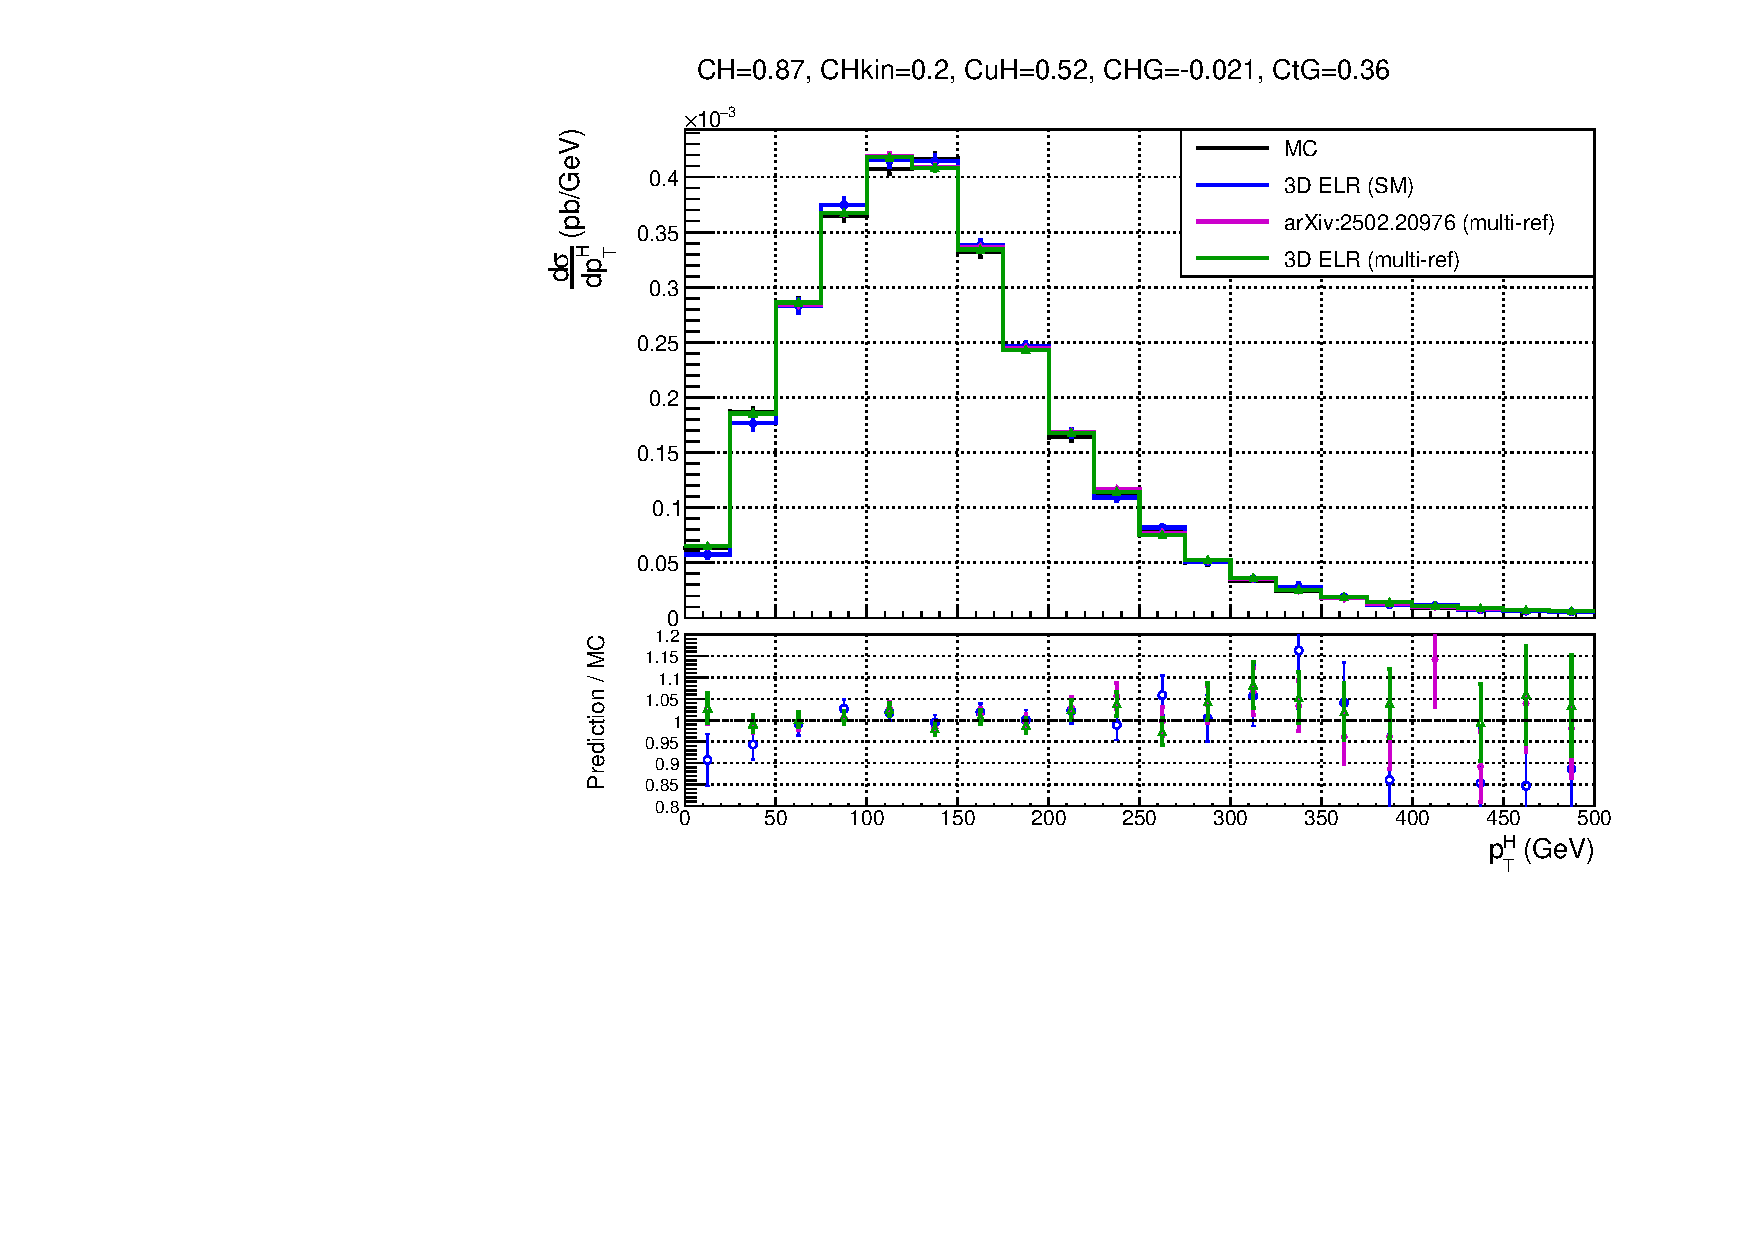
\includegraphics[width=\linewidth]{plots/pth_3d_SM_vs_multiref_vs_Luca_(71)_CH_0.874886_CHbox_0.201155_CuH_0.515566_CHG_-0.0206212_CtG_0.360217_CQt_0.0_CQt8_0.0_CQQtt_0.0_CQQ8_0.0.pdf}
  \end{minipage}
  \hfill
  \begin{minipage}[b]{0.495\linewidth}
    \centering
    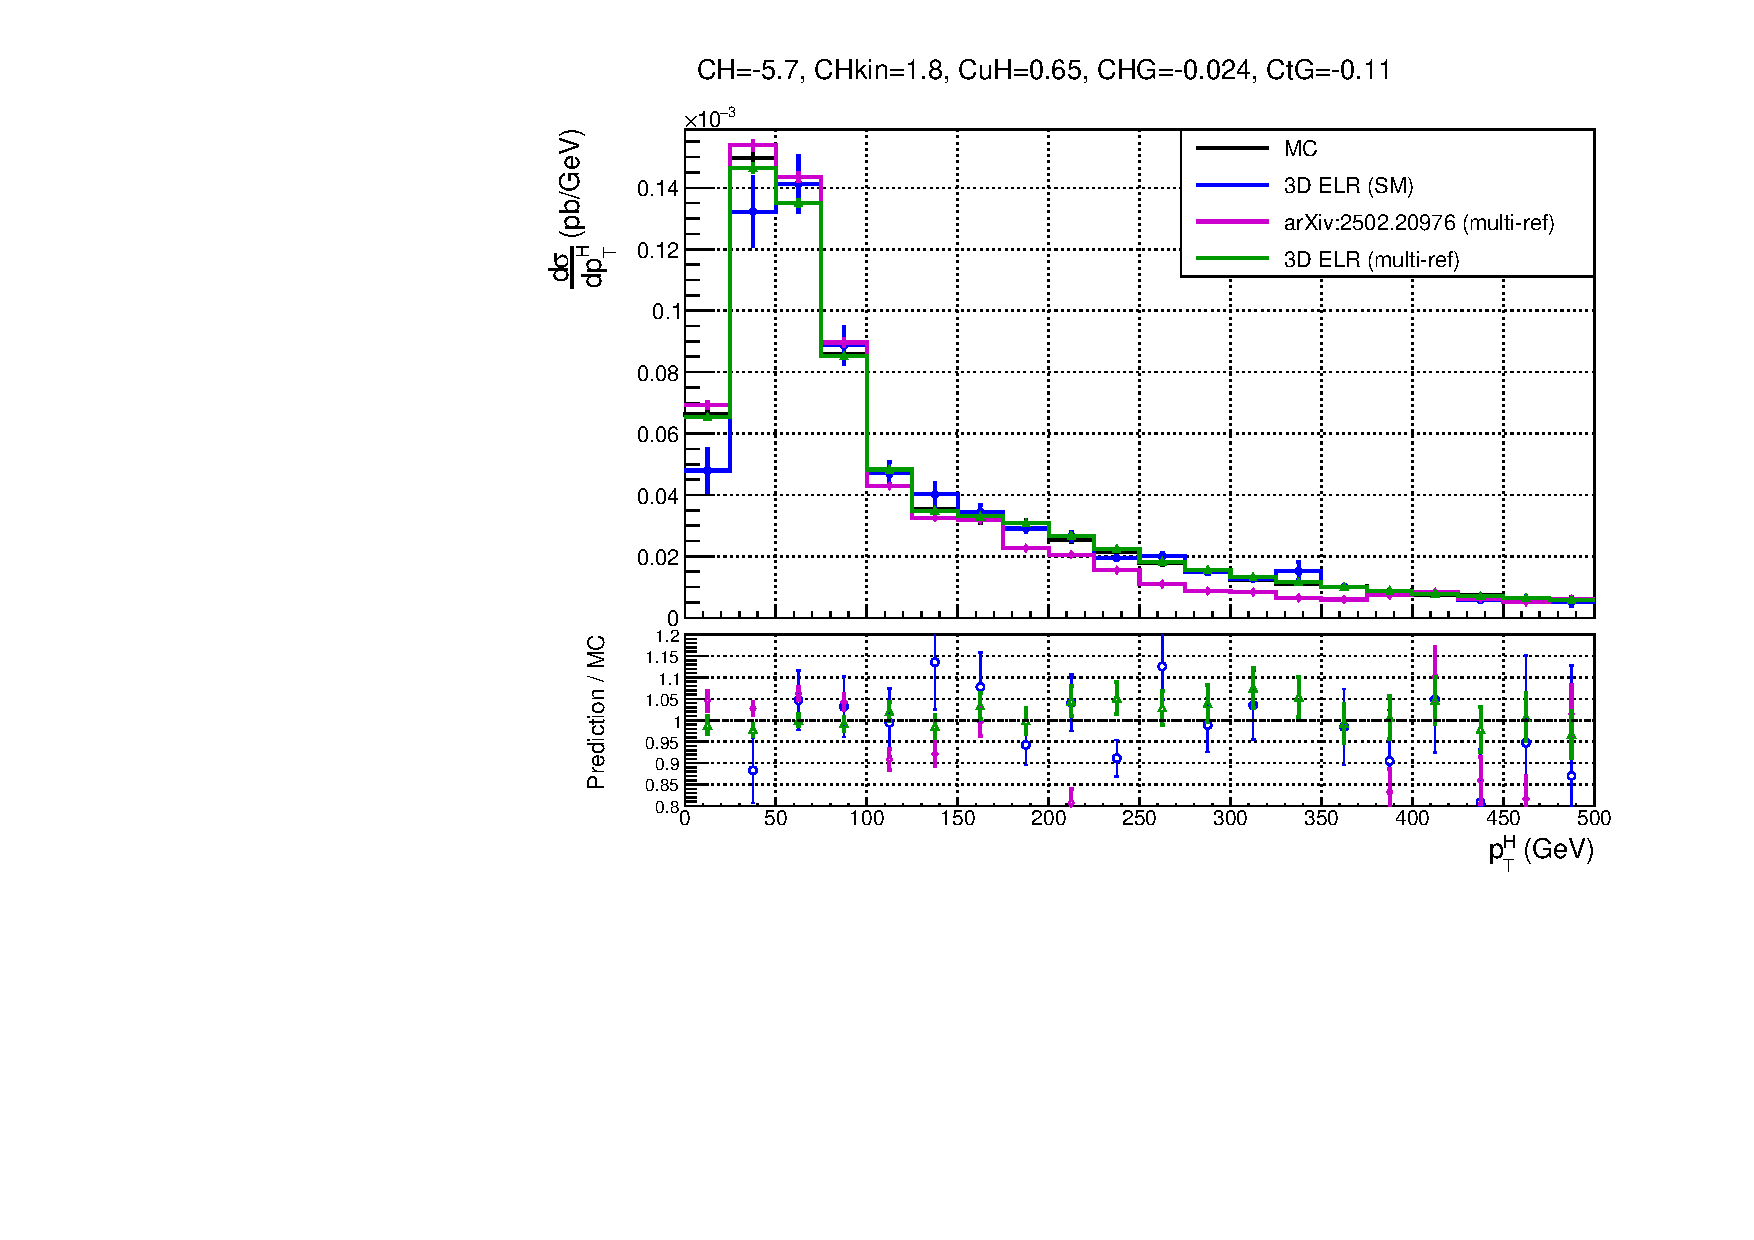
\includegraphics[width=\linewidth]{plots/pth_3d_SM_vs_multiref_vs_Luca_(19)_CH_-5.72209_CHbox_1.76334_CuH_0.653559_CHG_-0.0238598_CtG_-0.10625_CQt_0.0_CQt8_0.0_CQQtt_0.0_CQQ8_0.0.pdf}
  \end{minipage}
  \vspace{0.5em}
  \begin{minipage}[b]{0.495\linewidth}
    \centering
    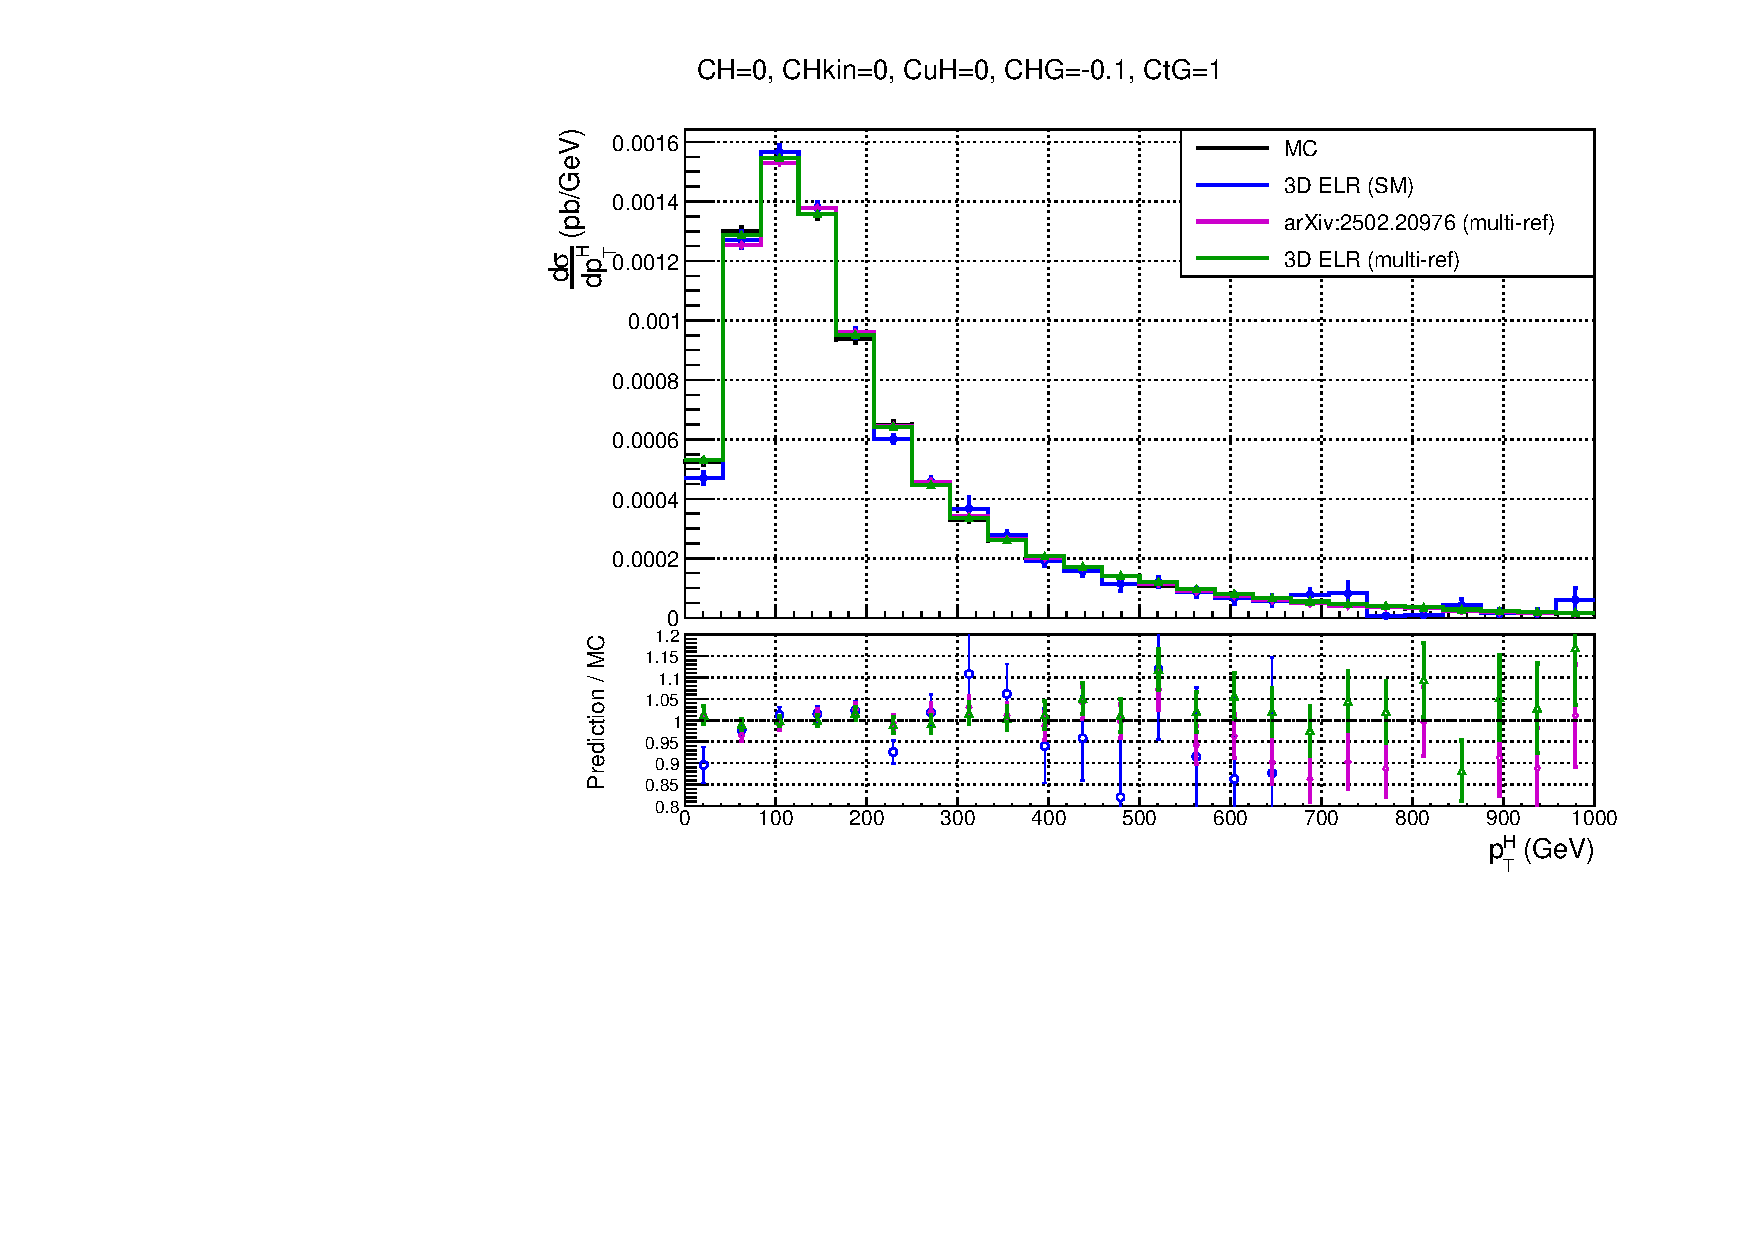
\includegraphics[width=\linewidth]{plots/pth_3d_SM_vs_multiref_vs_Luca_(30)_CH_0.0_CHbox_0.0_CuH_0.0_CHG_-0.1_CtG_1.0_CQt_0.0_CQt8_0.0_CQQtt_0.0_CQQ8_0.0.pdf}
  \end{minipage}
  \hfill
  \begin{minipage}[b]{0.495\linewidth}
    \centering
    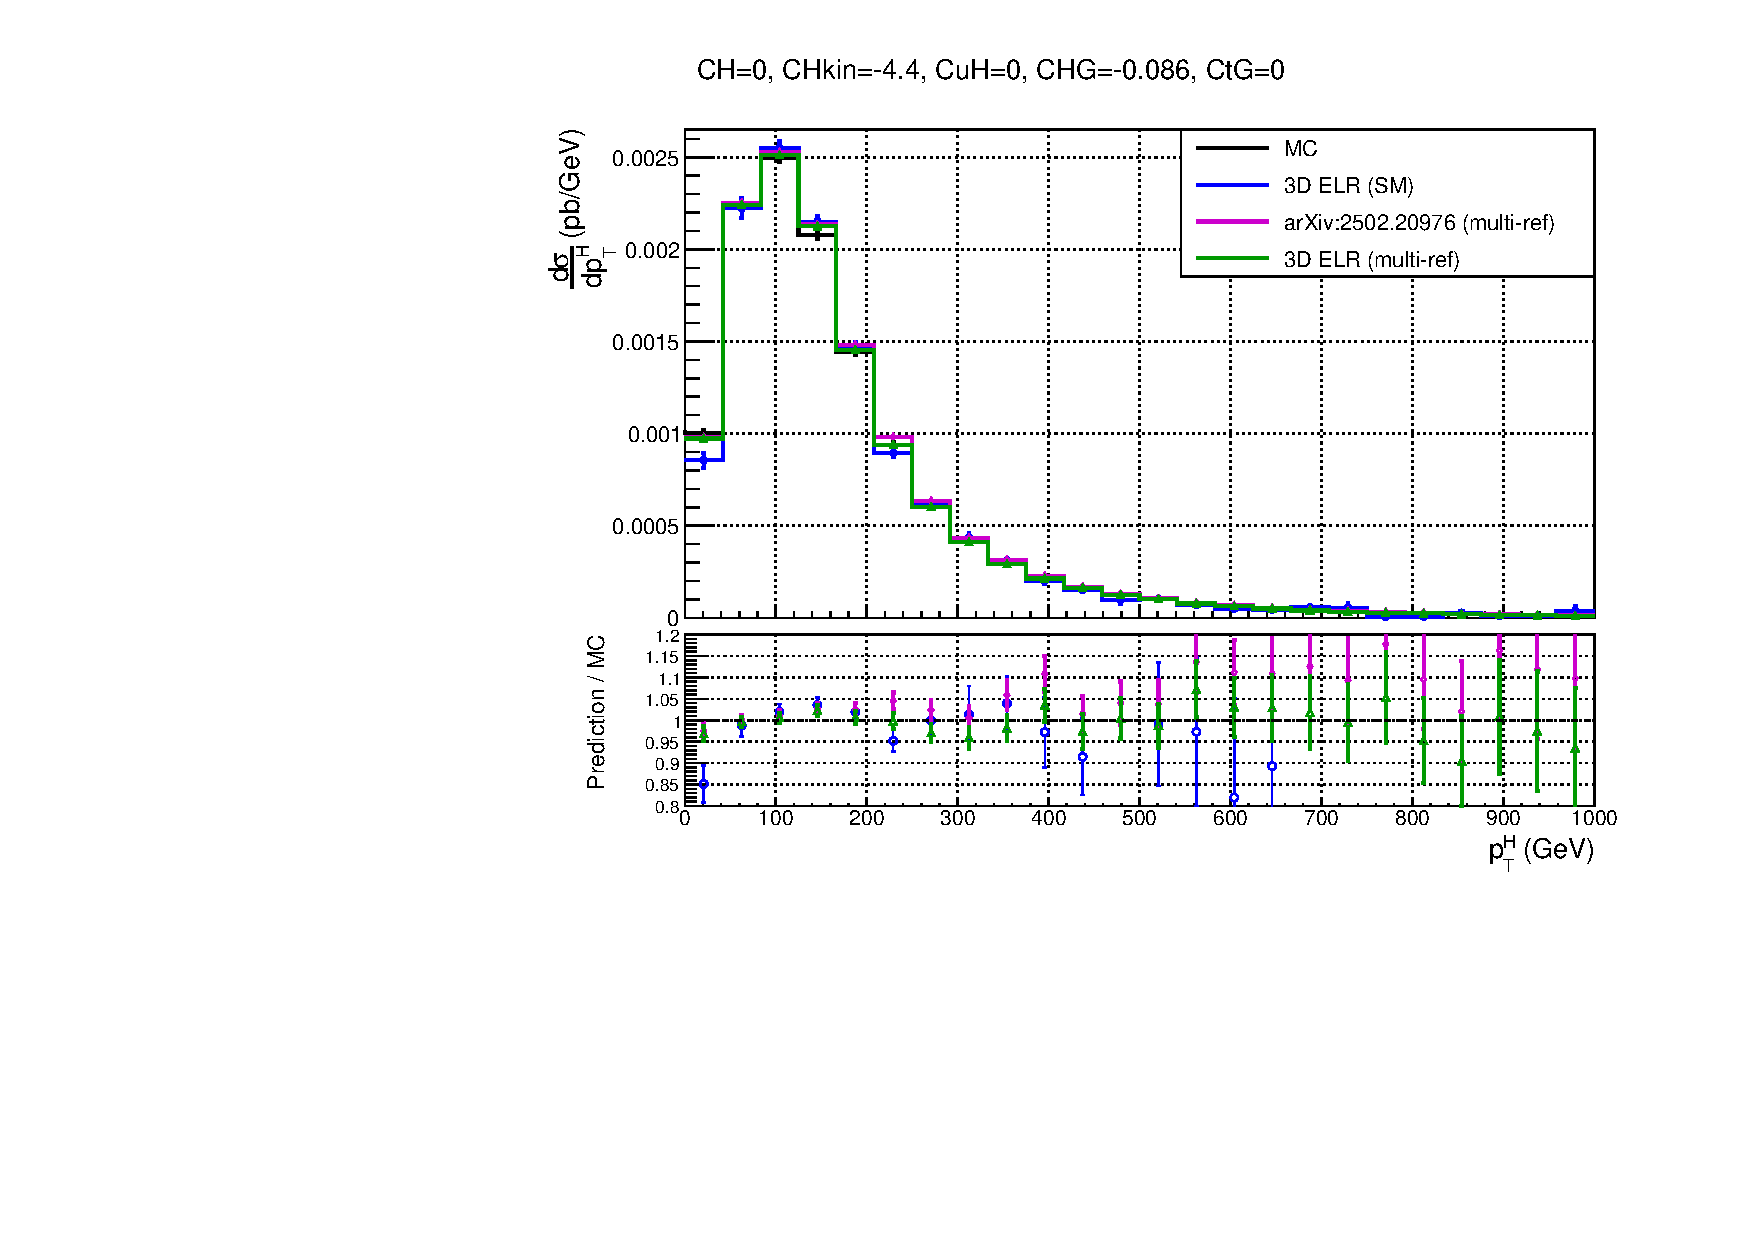
\includegraphics[width=\linewidth]{plots/pth_3d_SM_vs_multiref_vs_Luca_9_CH_0.0_CHbox_-4.44444_CuH_0.0_CHG_-0.0855556_CtG_0.0_CQt_0.0_CQt8_0.0_CQQtt_0.0_CQQ8_0.0.pdf}
  \end{minipage}
  \caption{Some of the test-samples probing the $\{c_\PH,\,c_{\PH \mathrm{kin}},\,c_{u\PH},\,c_{\PH G},\,c_{\PQt G}\}$ subspace. 3D ELR (multi-ref) shows stable modeling in the whole parameter space, also improving the precision in the boosted region, as indicated by the bottom plots.}
  \label{fig:pth}
\end{figure}
\begin{figure}[h!]
    \centering    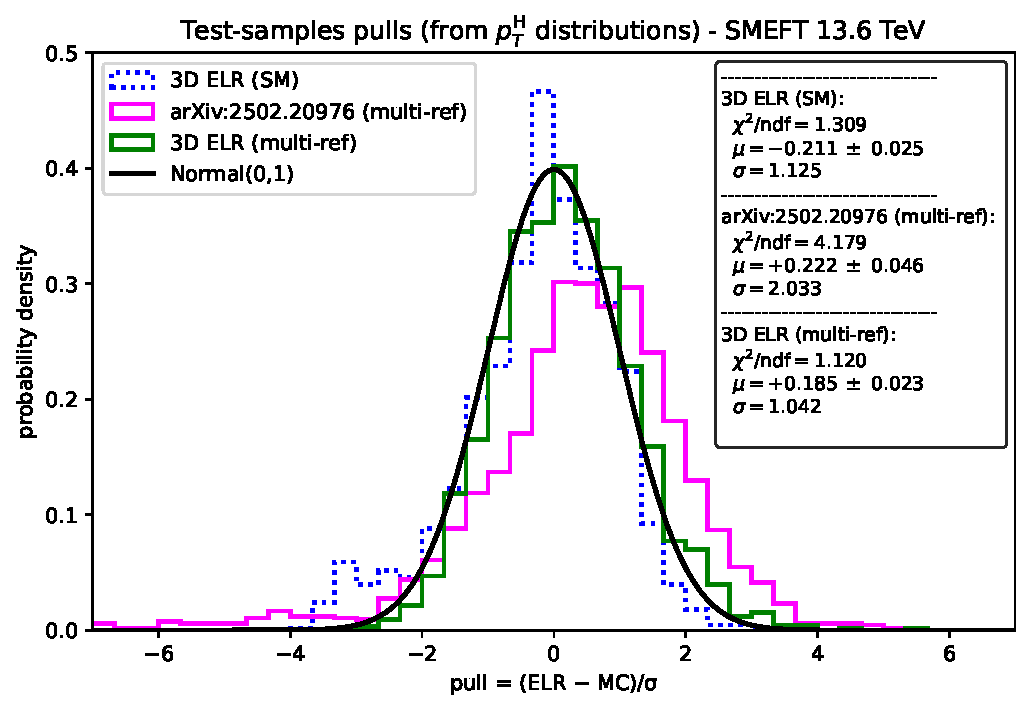
\includegraphics[width=0.8\linewidth]{plots/combined_pth_3d_SMEFT_test_plot_multiref_LUCACOMP_50_1.pdf}
    \caption{Pull distribution and statistical parameters obtained using all test-samples in all $p^\text{H}_T$ bins in SMEFT. We show the $\chi^2_\text{red}$, and the mean ($\mu$) calculated from all pulls, with its error given by $\sigma/\sqrt{N}$, for $\sigma$ the corresponding standard deviation.}
    \label{fig:stats}
\end{figure}
%Two parameterizations are provided: a 1D one differential in \mHH, and a 3D one differential in $\{m_{hh},|\cos\theta^*|,p^{hh}_T\}$. The 1D formula gives the best description of the \mHH shape itself, while the 3D one is the appropriate choice when other kinematic variables have to be reweighted, or when the shape is built after experimental selections, since $p^{hh}_T$ encodes the non-linear effects that such selections induce.

%Independently of the binning, the $A$-coefficients are extracted for two operator sets, from the two grids of Sec.~\ref{sec:grids}. The \emph{9D} parameterization determines all 40 coefficients of Eq.~\eqref{eq:smeftpara_reorg} from the 9D grid and is the \textbf{nominal} result: it is complete, in that it remains valid when the four-fermion operators are switched on, and it is the more stable of the two, the full operator space being populated by the samples. The \emph{5D} parameterization is a reduced fit that keeps only the leading operators together with $c_{\PQt G}$---i.e. the coefficients $A^j_0$--$A^j_{14}$ and the $c_{\PQt G}$ entries of the linear and mixed brackets, with the remaining subleading coefficients set to zero---and is extracted from the 5D grid. It is provided \emph{only for comparison studies}: it is used to check that restricting the operator space leaves the leading coefficients and the reweighted \mHH shapes statistically compatible with the nominal determination, and it does not enter the central results. The comparison of the two is reported in Sec.~\ref{sec:validation}.

%The binning used to extract the formulas is given in Table~\ref{tab:binedge}. As in the HEFT case, the 3D binning is used only in the low-mass region ($m_{hh}<1000$~GeV) and a 1D binning is kept above it, where the number of events per bin would otherwise become too small.

%For the 1D coefficients a per-bin weighted least squares (WLS) fit is used, with every sample having at least one entry in a given bin contributing. For the 3D coefficients the weights are clipped to lie between $0.001$ and $100$ times the median weight of the corresponding bin, which prevents the highest-statistics samples from dominating and washing out the regions where the destructive interference between diagrams is strongest. The motivation and the comparison against the unclipped and iterative alternatives are given in Ref.~\cite{ELR_R5}.


%The $A$-coefficients are extracted independently at each of the three centre-of-mass energies, since the parameterization is a statement about cross sections and the coefficients absorb the energy dependence of the process. Figures in this report show the $13.6$ and $100$~TeV results; the $13$~TeV ones are close enough to the $13.6$~TeV ones that showing them adds nothing, and are provided with the ancillary material.


\subsection{Implementation in the \texttt{ELReweighter}}
\label{sec:elr_implementation}


All the coefficients derived in this work are included in the \texttt{ELReweighter} package presented in Ref.~\cite{ELR_R5}. The tool allows for the ELR of any target point in the SMEFT 9D parameter space. For a given input sample "i", the following weight can be used for building any differential distribution:
\begin{equation}\label{ELReweighter}
    w_i=\frac{Poly(\mathbf{c}^{\text{target}}, \mathbf{A}^j)}{Poly(\mathbf{c}^{\text{input}}_i, \mathbf{A}^j)},
\end{equation}
where $j$ corresponds to a given bin among those shown in Table~\ref{tab:binedge}. The propagated uncertainties consider the statistical error of the input sample and the covariance matrix of the $A$-coefficients. The multi-ref approach is integrated in the \texttt{ELReweighter}, thus several input samples can be used at once. Each provides an estimate of the target distribution from its own events, and the estimates are combined bin-by-bin with weights given by the inverse of their statistical variance, so that every input contributes where its \mHH spectrum is populated.

Any input sample can be used provided the generator-level weights, the HH kinematics and the total cross section are given. The \texttt{ELReweighter} also supports HEFT, therefore HEFT samples can be used as input samples---i.e. the denominator in equation \eqref{ELReweighter}---to generate SMEFT distributions, and vice-versa. In particular, the templates of Sec.~\ref{sec:validation_realistic} are produced this way: four samples generated at different values of $\kappa_\lambda$, in HEFT, supply the whole nine-dimensional SMEFT space. 


%In particular, for investigating both ELR and the matrix method---to be discussed in the next Sections---in SMEFT and in the signal region of recent Run 3 measurements, we refer to the information released by the CMS Run 3 \HH$\to b\bar b b\bar b$ search \cite{CMS:2026znu}, available in the HEPData format \cite{hepdata.171917,Maguire:2017ypu}. The material contains all the experimental selections applied to generator-level events, for four $\kappa_\lambda$ scenarios: $\kappa_\lambda=0,\,1,\,2.45,\,5$. This is done separately for two of the topologies explored in the search, namely resolved, and merged. While the former targets the regime where the four $b$-quarks can be individually reconstructed without overlapping, the latter aims the case where the $b$-jets are produced highly collimated, therefore leaving two large merged jets in the calorimeter. The distributions are used as input to the \texttt{ELReweighter} tool, and are further used 

%the templates of Sec.~\ref{sec:validation_realistic} are produced this way: four samples generated at different values of $\kappa_\lambda$, in HEFT, supply the whole nine-dimensional SMEFT space






%Every result of this report that involves a selection---the acceptance scans of Sec.~\ref{sec:validation_realistic} and the templates the matrix method is built on---is produced with it.
%The coefficients of this section are released in the \texttt{ELReweighter} package of
%Ref.~\cite{ELR_R5}, together with the application recommended here. That package is the
%same one the HEFT report uses; what changes is the parameterization it is given, not the
%machinery. As in Ref.~\cite{ELR_R5} for HEFT, the recommended use is \emph{multi-reference}:
%several input samples reweighted to the same target and combined, rather than one. The
%evidence for that recommendation, and the number of inputs it takes, are in
%Sec.~\ref{sec:validation_nsamples}.

%The tool turns
%an existing simulated sample into a prediction at an arbitrary coupling point by
%reweighting it event by event. The weight of an event is the ratio of the differential
%cross section at the target point to that at the point the sample was generated at,
%evaluated in the $(\pt^{\HH}, |\cos\theta^*|, \mHH)$ cell the event falls in,
%
%\begin{equation}
%w(e) = \frac{\sigma_{\text{t}}(\mathbf{c}_{\text{t}};\,\text{cell}(e))}
%            {\sigma_{\text{in}}(\mathbf{c}_{\text{in}};\,\text{cell}(e))} ,
%\label{eq:elr_weight}
%\end{equation}
%
%with $40$ \mHH bins times the $\pt^{\HH}$ and $|\cos\theta^*|$ bins of
%Table~\ref{tab:binedge}, $1090$ cells in total. The normalization of each input sample is
%taken from its own metadata, as the generator weight times the sample cross section
%divided by the sum of generator weights.

%The input samples need not be generated in the model of the targets. The numerator of
%Eq.~\eqref{eq:elr_weight} is taken from the SMEFT parameterization of this report and the
%denominator from the parameterization of the model the sample was produced in, both
%fitted on the same cells. An input is read in its own couplings only: it is never placed
%in the SMEFT space, and no relation between the coupling modifiers of one model and the
%Wilson coefficients of the other is used. The reweighting uncertainty is that of the
%numerator, propagated from the covariance of the SMEFT coefficients.

%Several input samples can be used at once. Each provides an estimate of the target
%distribution from its own events, and the estimates are combined bin by bin with weights
%given by the inverse of their statistical variance, so that every input contributes where
%its \mHH spectrum is populated. The templates of
%Sec.~\ref{sec:validation_realistic} are produced this way: four samples generated at
%different values of $\kappa_\lambda$, in the $\kappa$ framework, supply the whole
%nine-dimensional SMEFT space.

%The procedure is validated against the one point for which a generated SMEFT sample
%exists. After the resolved $\HH\to\bbbar\bbbar$ selection the SM prediction
%built from the four inputs gives an acceptance times efficiency of $6.06\%$, against
%$6.05\%$ for the generated SM sample histogrammed directly. Each input taken
%alone reproduces the same template to within $1\%$ for $\kappa_\lambda = 0$ and $2.45$ and
%$4\%$ for $\kappa_\lambda = 5$, the last reflecting that the stated cross section of that
%sample is $4\%$ higher relative to the $\kappa$ parameterization than the others'. A
%further check is available to any analysis using this procedure: the SM point
%of a SMEFT table has to agree with the SM point of a $\kappa$ table built from
%the same inputs, since the two describe the same physical point and the second is reached
%without the SMEFT reweighting.



\clearpage
\section{The matrix method and the choice of basis}
\label{sec:matrix}

\label{sec:matrixmethod}

Reweighting removes the cost of simulating each parameter point, but not the cost of pushing each resulting template through the full experimental analysis chain, which remains prohibitive for a scan over nine Wilson coefficients. The matrix method removes that second cost, allowing, for instance, shape systematic uncertainties to be evaluated only over a subset of basis points (BPs) and then extrapolated to the full theory space. Since the cross section is linear in the $A$-coefficients, any (differential) cross section can be rewritten as a linear combination of the cross sections at a fixed set of BPs,
\begin{equation}
    \sigma_\ggHH(\mathbf{c})=\vec{c}^{\,\top}(\mathbf{c})\cdot C^{-1}(\mathbf{c}^\prime_1,\,\mathbf{c}^\prime_2,\,\cdots)\cdot\vec{\sigma}_\ggHH(\mathbf{c}^\prime_1,\,\mathbf{c}^\prime_2,\,\cdots)\;,
    \label{eq:matrixmethod}
\end{equation}
where $C$ is the matrix of coupling terms evaluated at the BPs. Only those basis templates then have to be processed through the analysis, and every other point of the parameter space is obtained as a linear combination of them. With the 40 coupling combinations of Eq.~\eqref{eq:smeftpara_reorg}, a minimal basis consists of 40 points. While the matrix method is also discussed in Refs.~\cite{HH_nonggf_R5,HHMatrix_R5}, here the goal is to find an appropriate set of 40 BPs in SMEFT. In view of the aforementioned references, two approaches can be listed:

\begin{itemize}
    \item Ref.~\cite{HHMatrix_R5} uses the $A$-coefficients to throw \emph{toy} \mHH templates, and then searches the BPs with a particle swarm optimization over a continuous hyperparameter space. This is the appropriate choice when no sample set exists yet, as the $A$-coefficients provide a cheap way to produce $m_{\HH}$ shapes. No simulation needed.
    \item Ref.~\cite{HH_nonggf_R5} scores candidate bases directly on \emph{simulated} samples, and searches by iteratively exchanging one basis point at a time among the available samples. %This is the appropriate choice when a large set of simulated samples already exists.
\end{itemize}

We follow the approach of Ref.~\cite{HH_nonggf_R5} here, for two reasons. First, the samples needed are already available: the same $4500$ SMEFT samples generated at $13.6$~TeV for the extraction of the $A$-coefficients in Sec.~\ref{sec:extraction} can be reused as input to the basis search and as target distributions, as well as for validation purposes. Second, the LHE-based evaluation allows for an easy treatment of the statistical error, which are otherwise emulated in the toys used in Ref.~\cite{HHMatrix_R5}.


%Ref.~\cite{HHMatrix_R5} found that the toy-based templates, being built from a simplified model of the process, do not reproduce the statistical behaviour of genuine events: the relative statistical error evaluated on toys is systematically shifted with respect to the one evaluated on LHE events, and the LHE-based evaluation is the more faithful of the two. Since the statistical term is one of the quantities the basis search is meant to control, scoring directly on LHE events avoids optimizing against a proxy. It also makes the closure uncertainty of Sec.~\ref{sec:uncertainties} derivable differentially, which the toy-based route does not allow.

%\subsection{Basis optimization and two-dimensional scan planes}
%\label{sec:basisopt}

%The basis search follows Refs.~\cite{HHMatrix_R5,HH_nonggf_R5} and we only recall its ingredients. 

Candidate bases are ranked by a total score combining three closure terms: a shape term built from the cumulative-distribution and Hellinger distances between the generated and interpolated spectra, a rate term on the inclusive cross section, and a bin-by-bin term taking the 90th percentile of the per-bin relative errors. Then, three stability penalties are set: the condition number of the scaled basis matrix, the magnitude of the interpolation weights, and the fraction of negative interpolated bins. The search itself starts from several seed configurations and proceeds by exchanging one basis point at a time, accepting an exchange when it improves the total score, with the best seed retained.


Provided the cross section terms are given by linear and quadratic pieces, we restrict the BPs to be at most two-dimensional and use the 2D points mentioned in Table~\ref{tab:grids_comp} as the parameter space seeding the BP search---then every one of the $40$ points of the recommended basis lies in a plane, with thirty-nine having exactly two non-zero coefficients and one being the SM. All the remaining samples varying more than two Wilson coefficients are used as targets to which every candidate basis is scored against. In order to test the 2D scan approach, we allow a few exceptions with more than two non-zero Wilson coefficients and compare the results with the basis containing only 2D BPs. The latter outperforms other alternatives in the relevant metrics (condition number, median shape residual, etc) and is therefore the chosen approach. Additional comments concerning overdetermined bases, the trajectory of different seeds, and so on, are discussed in Appendix~\ref{sec:appendix_basis_search}.

Experimental analyses are often designed to also cover other SMEFT truncations and operators, requiring dedicated bases tunned to each of the probed scenarios. For instance, a modeling covering only the leading operators in the quadratic truncation would require 15 BPs, and those can be achieved with a similar approach to the one described in this Section. In view of that, dedicated BPs were also derived for the following cases: linear truncation and leading operators, quadratic truncation and leading operators, quadratic truncation and leading operators plus the chromomagnetic operator. In the following Sections, however, we focus on the 40 BPs required for SMEFT at the quadratic truncation with all the subleading operators.

%\subsection{Restricting the basis to the two-dimensional scan planes}
%\label{sec:basis_planes}

%Most points of the grids of Sec.~\ref{tab:grids_comp} lie in one of the $\binom{9}{2}$ planes
%in which a single pair of coefficients is varied with the rest at their SM values, and we
%require the basis points to be drawn from those planes. The restriction is on
%\emph{membership} alone --- on which samples may enter a basis, not on which are used to
%find it. The off-plane samples, two thirds of the grid, are the targets every candidate
%basis is scored against, and they are what decides which basis is chosen. The restriction
%is not an approximation: no monomial of Eq.~\eqref{eq:smeftpara_reorg} involves more than two
%distinct coefficients, so a set of points each activating at most two of them is not
%structurally degenerate.



%%%%%%%%%

%What decides this is the number of distinct couplings a single term contains, not the
%degree. A point that activates two couplings gives a non-zero value only to
%monomials built from those two, so a monomial involving three distinct couplings would
%leave an identically zero column in the design matrix and no set of two-coupling points
%could span the space. A high power of one coupling is no obstacle; a product of three is.

%The dimension-6 cross section is an interference and a square of amplitudes each linear
%in the Wilson coefficients, so every monomial here involves at most two of them, and the
%restriction is exact. The HEFT parameterization of the same process does not have that
%structure: its terms reach three distinct couplings at once, at total degree four, so the
%plane restriction is unavailable there even though it involves fewer couplings in all.

%Every one of the $40$ points of the recommended basis lies in a plane: thirty-nine
%activate exactly two coefficients and one is the SM. Allowing two points off the planes,
%tested as a separate twenty-seed sweep, gives a score of $0.624$ against $0.609$, a
%median relative shape residual of $3.5\%$ against $3.0\%$, and a condition number of
%$26.6$ against $32.7$. Each basis point then isolates one coefficient pair, which is the
%form the results are presented in.

%The loss asks a candidate basis to predict every other sample in the grid, and at
%$13.6$~TeV $2792$ of the $4376$ samples activate more than two coefficients. Scoring
%against the on-plane samples alone would select a different basis:
%Appendix~\ref{sec:appendix_basis_planes} gives that measurement, together with the
%numerical and interpretational arguments for restricting the membership.

%\subsection{Refinements to the search}
%\label{sec:basis_refinements}

%The search is the one of Ref.~\cite{HH_nonggf_R5} and we have not changed its
%objective: the same six-term score, the same single-point exchange, the same
%sweep over random seeds with the lowest-scoring seed retained. The changes below are
%refinements to how the search is started and how large a parameter space it can
%be run in. They matter here because this report optimizes bases in up to nine
%dimensions against sample sets four to seven times larger than the one used in
%Ref.~\cite{HH_nonggf_R5}, and two of the steps that are harmless at five
%couplings and a few hundred samples are not harmless at nine.

%There are five. Randomly drawn starting
%configurations are redrawn until the interpolation matrix has full rank, because in nine
%dimensions $85\%$ of uniform draws are singular for a counting reason: $20$ of the $40$
%monomials vanish unless a four-fermion coefficient is non-zero, while only $45\%$ of the
%samples have one. The well-conditioned starting configuration is built so that it spans
%the monomials, not only so that it is well conditioned. The score is evaluated for all
%targets at once, which costs a factor of about five less and so keeps the full
%optimization set affordable at every exchange step, with no subsampling. More basis
%points than monomials are allowed as an option, the weights then being the minimum-norm
%least-squares solution, though the published bases are exactly determined. And the
%trajectory of every seed is recorded, which is what shows that a seed cannot be judged
%before it has converged. Appendix~\ref{sec:appendix_basis_search} gives each of these,
%together with what makes the problem tractable and the changes that did not improve it.


\clearpage
\section{Validation without selections}
\label{sec:validation}

%This section validates the parameterization and the basis on the generated samples
%themselves, with no selection applied. The behaviour under a realistic selection is the
%subject of Sec.~\ref{sec:validation_realistic}.

The basis search returns the basis with the lowest score, exhibited in Table~\ref{tab:smeft_basis_9d}, which can be further validated using all the generated samples not selected as BPs. Here the BPs are used in the matrix method applied to LHE events in the absence of any selection. The bin-level quantities of Ref.~\cite{HH_nonggf_R5} are used to investigate the accuracy of the modeling provided by the matrix method using the proposed BPs: the relative residual $(N_\mathrm{interp}-N_\mathrm{MC})/N_\mathrm{MC}$, the relative propagated interpolation uncertainty $\sigma_\mathrm{interp}/N_\mathrm{MC}$ of Eq.~\eqref{eq:sigmainterp}, and the pull $(N_\mathrm{interp}-N_\mathrm{MC})/\sqrt{\sigma^2_\mathrm{interp}+\sigma^2_\mathrm{MC}}$. Furthermore, with the savings in MC production time (ELR, $A$-coefficients) and computing resources required for the full experimental analysis workflow over a 9D scan (MM), the combination of both methods provides a crucial scheme for accessing the rich theory space of EFTs such as SMEFT, and is therefore explored in the upcoming sections. For the following tests, the shapes obtained solely from the $A$-coefficients serve as a reference baseline for the accuracy achieved with by the MM and MM+ELR approaches.

%but the score is a ranking
%device and not a statement about accuracy, and how well it stands in for one depends on
%the parameterization: over the seeds of a sweep its rank correlation with the held-out
%median shape error is $+0.61$ for the nominal nine-coefficient basis and $+0.07$ for the
%fifteen-point one, where it instead tracks the tail of the residual distribution. A
%finished basis is therefore validated separately from being selected. The validation
%uses the samples that are not themselves basis points --- $4336$ of them for the nominal
%parameterization --- so that nothing is scored on its own input, 

%with the bin-level quantities of Ref.~\cite{HH_nonggf_R5}: the relative residual $(N_\mathrm{interp}-N_\mathrm{MC})/N_\mathrm{MC}$, the relative propagated interpolation uncertainty $\sigma_\mathrm{interp}/N_\mathrm{MC}$ of Eq.~\eqref{eq:sigmainterp}, and the pull $(N_\mathrm{interp}-N_\mathrm{MC})/\sqrt{\sigma^2_\mathrm{interp}+\sigma^2_\mathrm{MC}}$.

\subsection{Kinematic behaviour of the basis points}
\label{sec:validation_shapes}
\label{sec:validation_nsamples}

The basis has forty points and can be sorted into four kinematic regimes. The number of regimes are separated according to the behavior of the shape at the interference regions $2m_{\text{H}}$ (threshold), $2m_{\text{t}}$, and in the high-mass tail. Normalizing each point to its own yield and grouping by the shape of the \mHH distribution, Fig.~\ref{fig:basis_shapes}, the same six structures highlighted in Ref.~\cite{Bär:2965348} are found. Such structures are given according to the rich diversity arisen from the interferences around the production threshold ($2m_\text{H}$) and $2m_t$, and also in terms of the similarity in relation to the SM shape. All the BPs found can be related to one of the six benchmarks defined in Ref.~\cite{Bär:2965348}.

%\footnote{Ref.~\cite{Bär:2965348} adds a new region where the contribution at $2m_{\text{H}}$ is not as suppressed as in the SM case. Here such samples are absorbed in what is quoted as "threshold-like". Furthermore, the "two peaks" region is also subdivided according to which peak ($2m_{\text{H}}$ or $2m_{\text{t}}$) is the dominant one.}. %It is well known that truncation effects can produce negative predictions in regions more sensitive to destructive interference between diagrams, and this can be seen in a small number of bins in Fig.~\ref{fig:basis_shapes}. Such effects are even more pronounced when restricted to the linear truncation, as just the SM-Dim6 interference is taken into account. Although unphysical, this is not a problem from the perspective of the modeling, are genuinely present in the kinematic space covered by the theory 

%. ...These come
%from the negative event weights of the next-to-leading-order generation where a sample has few events, they affect $0.5\%$ of bins, and they are not a truncation of the EFT expansion.

In a realistic scenario, the matrix method is often used together with the ELR: some of the BPs are directly produced with MC and then reweighted in a combined way to the remaining templates using bin-by-bin inverse-variance weights, namely the multi-ref approach discussed in Ref.~\cite{ELR_R5}. The identification of the shape properties helps to answer the question regarding which BPs must be chosen to be generated. The left panel in Figure~\ref{fig:elr_sources} shows the median relative shape residual as a function of the number of input points used in the ELR of all the remaining BPs required by the MM approach. Reference lines are drawn for the results obtained directly with the $A$-coefficients, and by the MM using all BPs directly generated by MC. The median is computed by comparing the shapes given by all three modeling techniques with all the generated samples (\ref{tab:grids_comp}), except for the BPs. The higher value given by the MM with 40 generated points is expected, as it carries the statistical fluctuations of each of the forty samples, something that is absent in the $A$-coefficients. By using the MM with points obtained through the multi-ref approach in an increasing number of BPs, the median drops towards the optimal value given by the $A$-coefficients, but saturates around six source samples, meaning that one BP representing each of the six kinematic groups sets an stable point to the MM+ELR approach. The particular combination of samples used in each of the blue markers starts first with the SM, since its the sample that any analysis generates anyway, and then proceeds by incrementally including any sample of the remaining five kinematic regimes once all of them are represented at least once. The right panel shows the shapes of the selected BPs used in the MM+ELR approach in the six-source point of the left panel. As expected, the effect of changing different BPs inside a given kinematic group it was found to be small. The distributions of the relative shape residual corresponding to the medians shown in Figure \ref{fig:elr_sources} are exhibited in Figure \ref{fig:closure_9d}, for the $A$-coefficients evaluated directly (blue), MM (orange), and MM+ELR (six sources, green).





%The matrix method can be used
%It is the number of regimes rather than the number
%of points that sets how many samples have to be simulated, which is what the rest of this
%subsection establishes.

%The regimes are separated by how much yield they place at high mass. Of each sample's
%yield, the fraction above $1$~TeV is $5.3\mbox{--}19.7\%$ for the hard-tail points,
%$0.0\mbox{--}7.2\%$ for the two-peak points, $0.0\mbox{--}4.9\%$ for the threshold-like
%points and $0.8\mbox{--}3.6\%$ for the SM-like ones, the SM itself at $0.8\%$. Above
%$1.2$~TeV the ordering holds with $3.2\mbox{--}13.7\%$, $0.0\mbox{--}3.3\%$,
%$0.0\mbox{--}2.4\%$ and $0.2\mbox{--}1.5\%$. A hard-tail point puts an order of magnitude
%more of its events where the spectrum is least populated than an SM-like one, so a set of
%samples covering the regimes constrains the tail better than one covering the coupling
%space uniformly.


\begin{figure}[htbp]
    \centering
    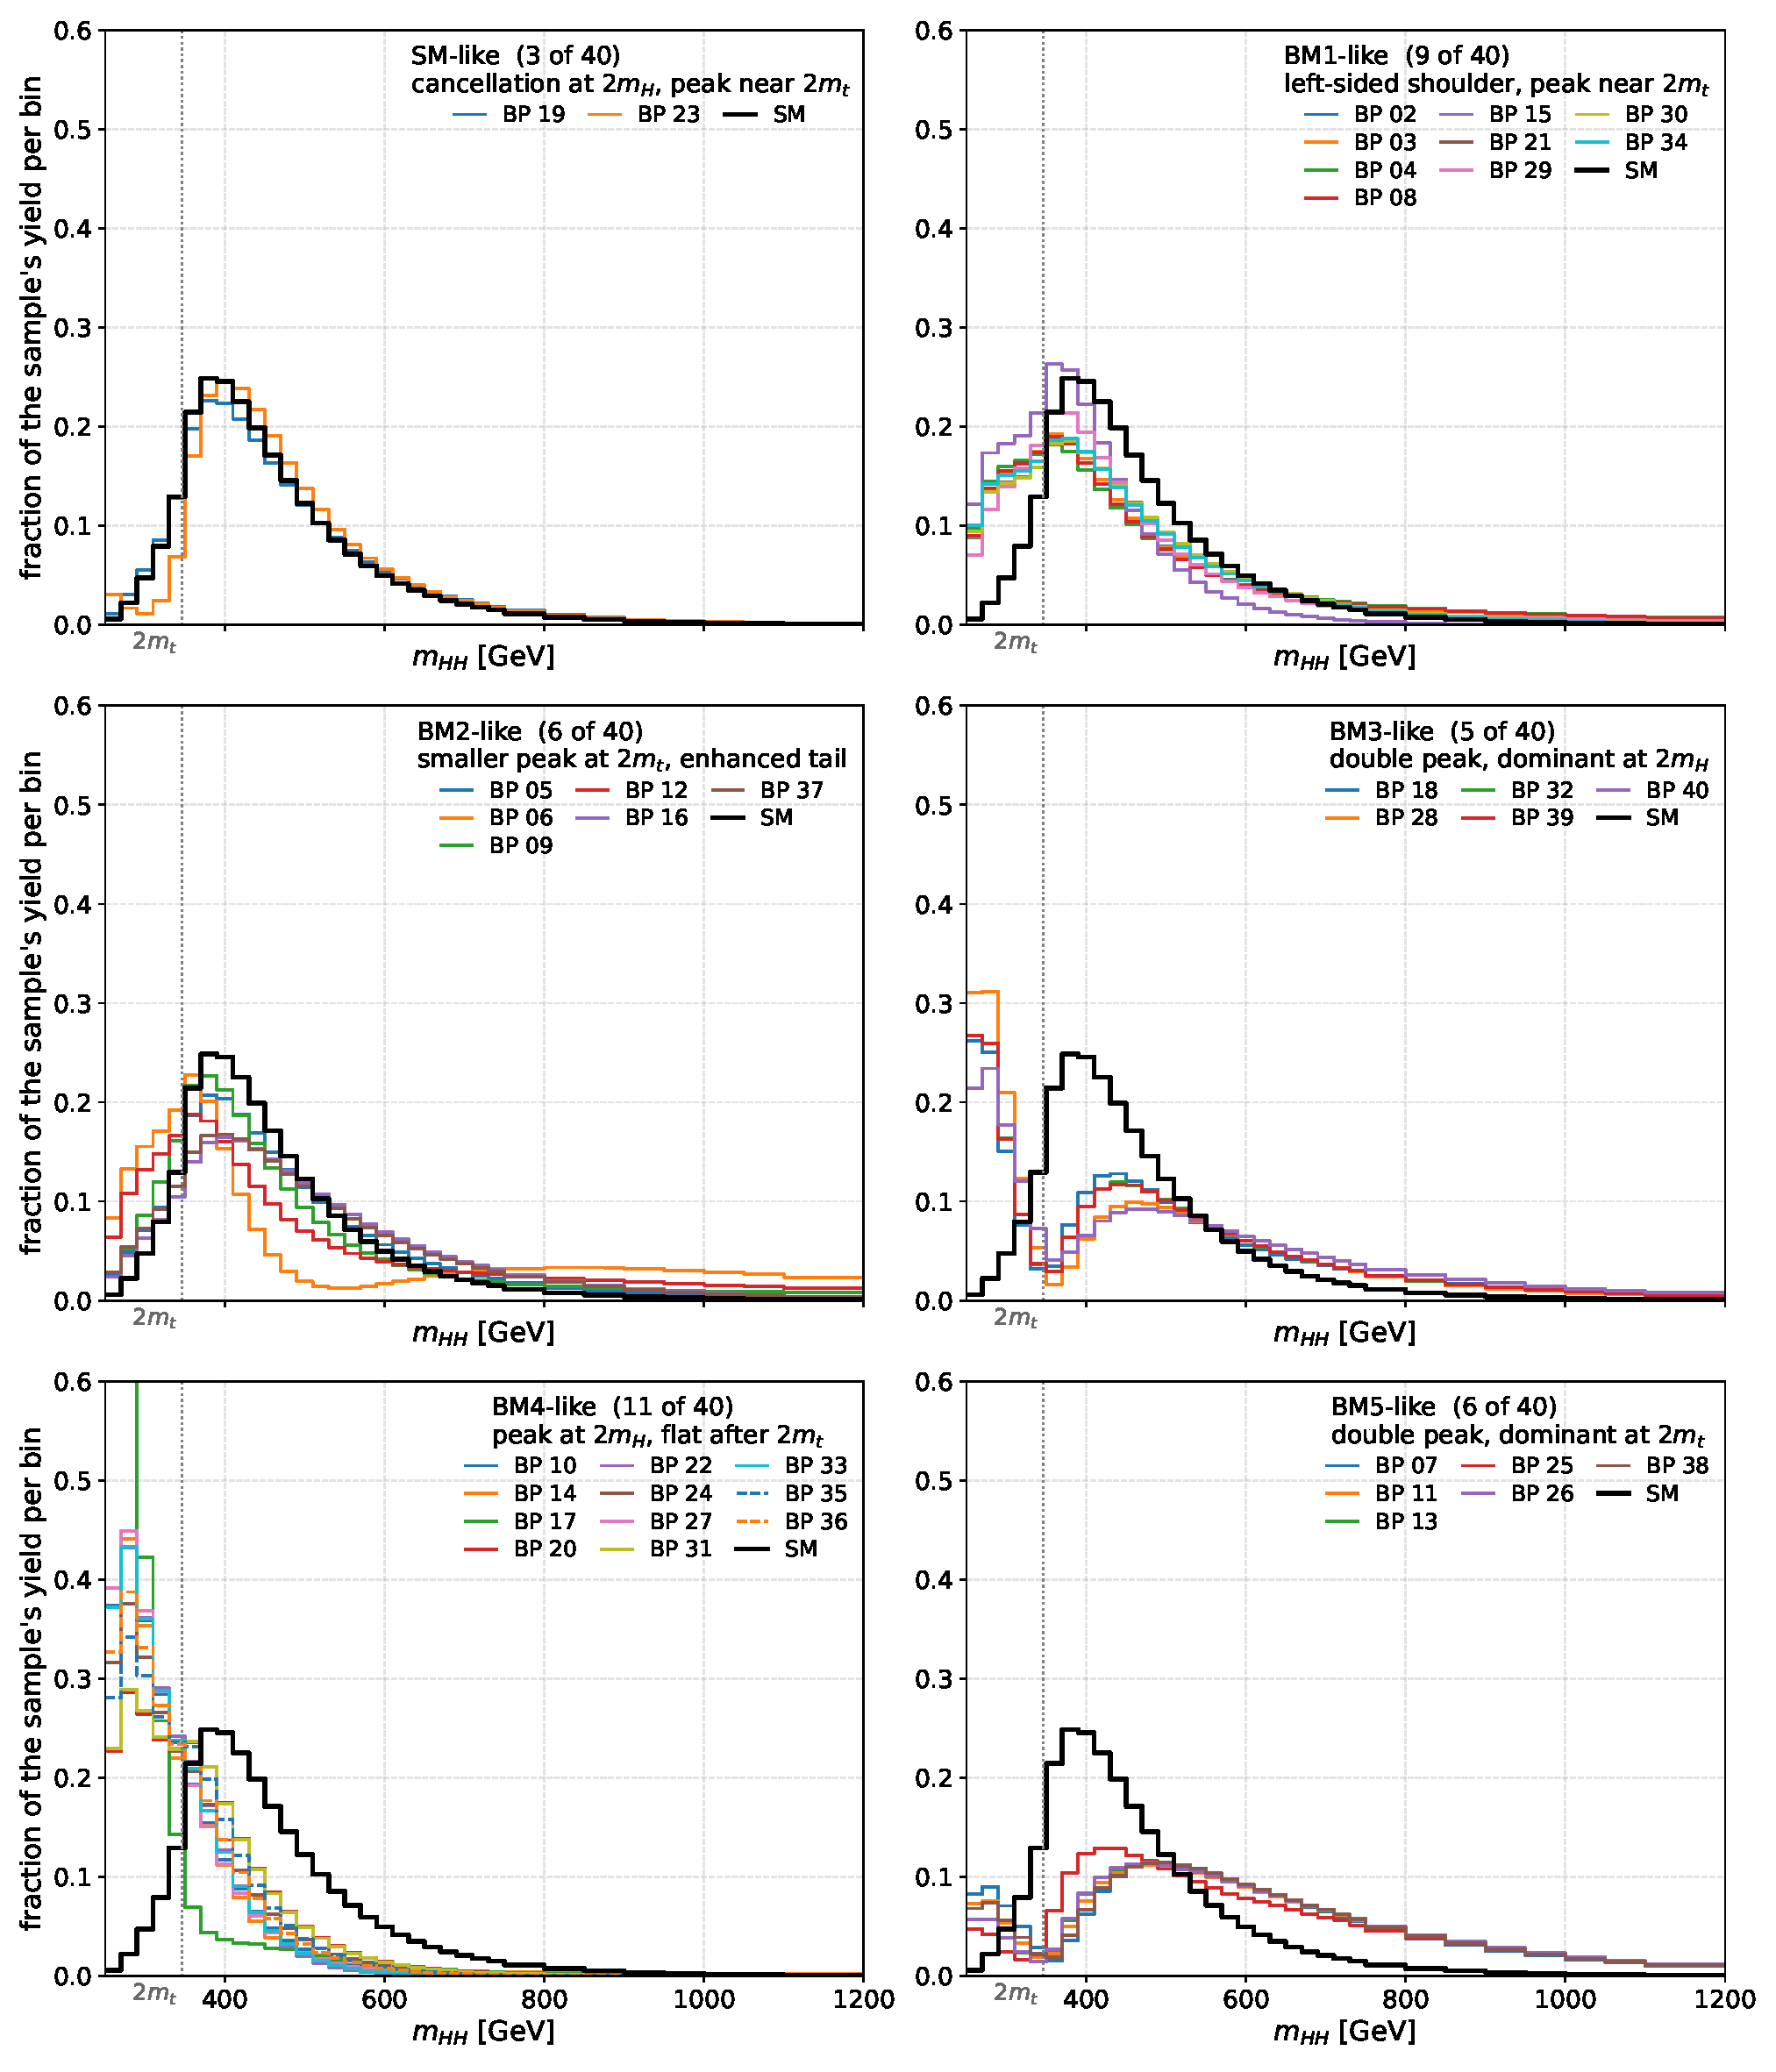
\includegraphics[width=1.025\textwidth]
        {plots/mHH_shape_classes_6panel_BMfeatures_newbasis_1.pdf}
    \caption{Normalized \mHH distribution of each of the forty basis points, grouped under each of the six identified shape features, with the SM drawn in black in every panel.}
\label{fig:basis_shapes}
\end{figure}
\begin{figure}[htbp]
    \centering
    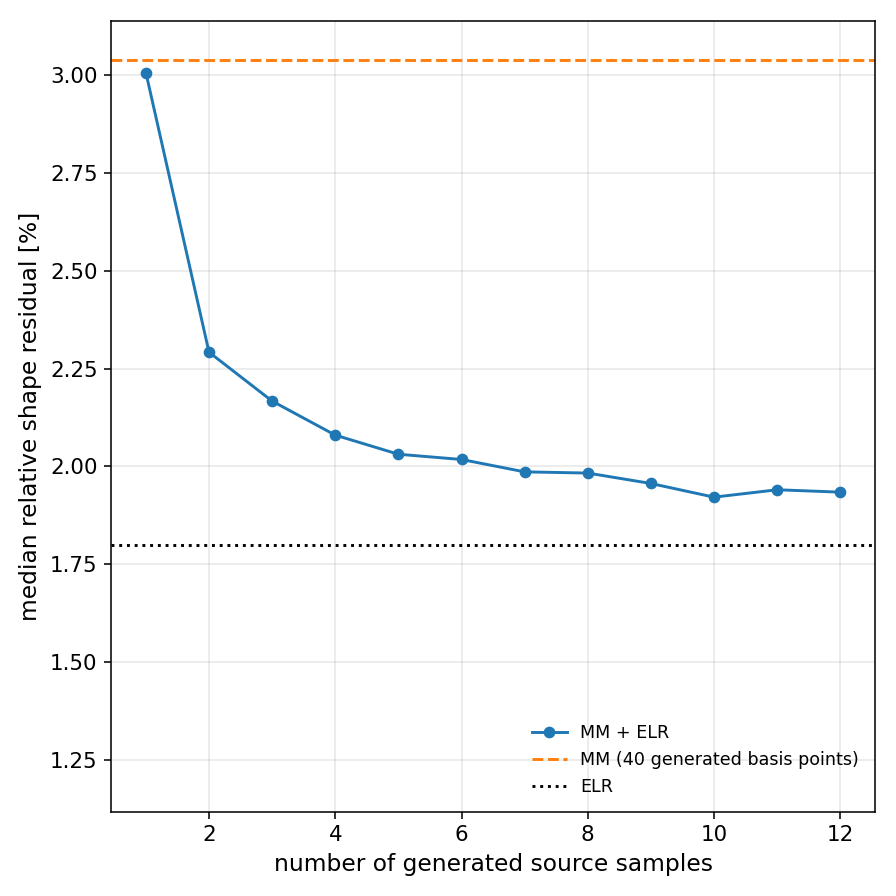
\includegraphics[width=0.47\textwidth]
        {figures/basis_optimization/elr_source_scan.png}
    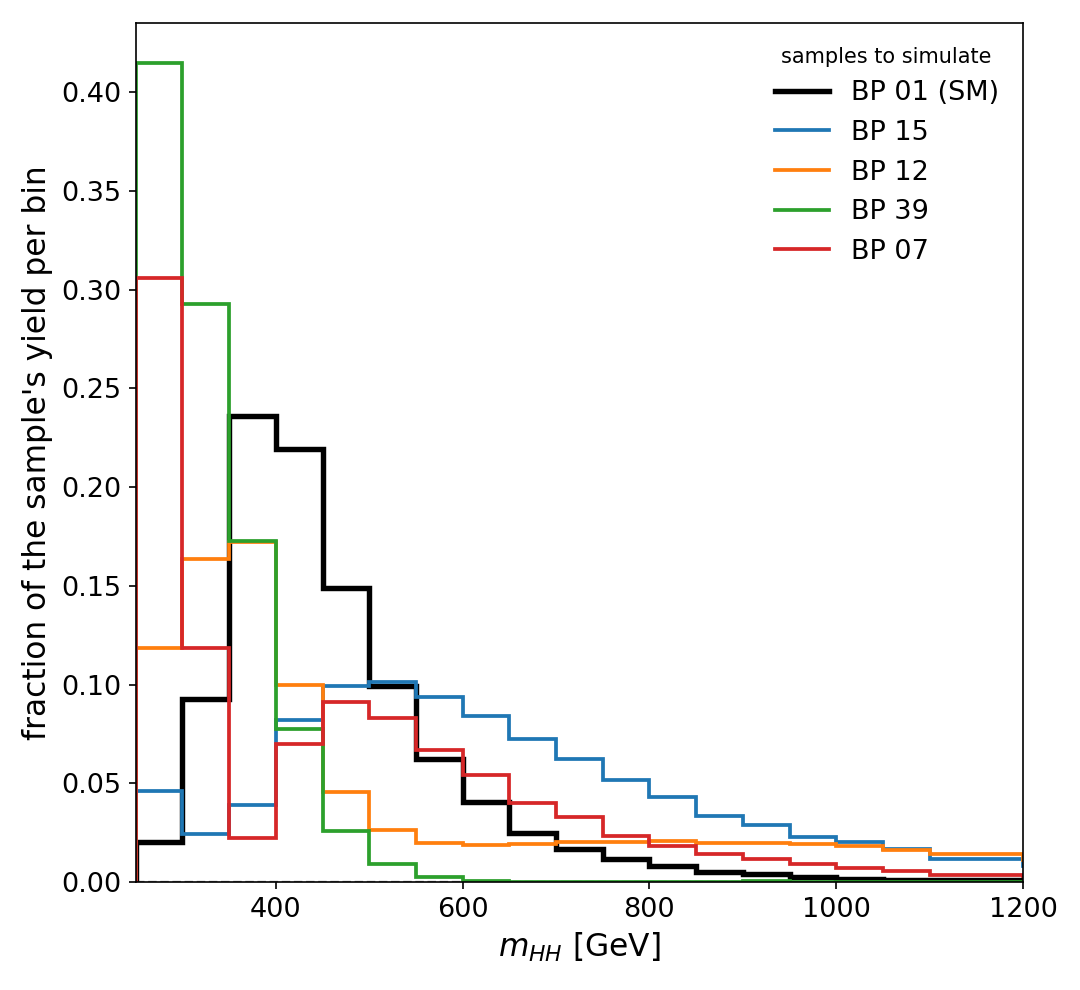
\includegraphics[width=0.51\textwidth]
        {figures/basis_optimization/elr_sources_5_mHH.png}
    \caption{Left: median relative shape residual of the forty-point basis when
    its templates are built by reweighting from a given number of generated
    source samples and combined per bin with inverse-variance weights, against
    the basis taken entirely from generated samples (dashed) and the distributions
    evaluated directly from the $A$-coefficients (dotted). Right: the \mHH distributions of the five
    samples used for the five-source point of the left panel, each normalized to its own yield.}
    \label{fig:elr_sources}
\end{figure}


%The residual of the matrix method is dominated by the statistics of its basis samples, so
%it is reduced by making those templates more precise. The price of doing that by
%simulation can be read off. Taking the reweighting fit evaluated at each basis point as a
%noise-free template and adding Gaussian noise of the size the real samples carry
%reproduces the delivered closure to about $15\%$ --- $3.5\%$ against the $3.0\%$
%observed --- and scaling that noise by $1/\sqrt{f}$ gives what $f$ times the events would
%deliver: $2.4\%$ at $f=5$, $2.2\%$ at $f=10$ and $2.0\%$ at $f=20$.

%The same precision is obtained instead by \emph{building} each basis template from a few
%simulated samples by reweighting, combined bin by bin with inverse-variance weights as in
%Ref.~\cite{ELR_R5}. The residual falls from $3.0\%$ with one source to $2.03\%$ with
%five, against $3.04\%$ with all forty simulated and a floor of $1.80\%$. Beyond five the
%improvement continues slowly --- $1.92\%$ at ten --- so the number to simulate is set by
%where the returns fall below the cost of a sample rather than by a plateau. The five
%sources are themselves basis points, so none of this asks for simulation outside
%Table~\ref{tab:smeft_basis_9d}. The left panel of Fig.~\ref{fig:elr_sources} shows the
%scan, approaching but not reaching the reweighting's own floor and lying below the
%$3.0\%$ of the basis as generated.

%Which samples are chosen is a smaller effect than how many, and it is set by the
%kinematics rather than by the coupling values. The five sources are drawn from the basis
%points, classified into the four regimes above. The SM is taken first, as the point
%every analysis simulates in any case; the remaining four are taken one regime at a time,
%and within a regime the point taken is the one furthest in normalized \mHH shape from
%everything already chosen, among those whose own statistics are no worse than half the
%median of the sample set. The order in which the regimes are visited is the one free
%choice, and weighting them equally is not the best rule: the hard tail is visited twice
%before the others are exhausted, because that is where the residual and its propagated
%uncertainty are largest, both growing by a factor $6\mbox{--}7$ between threshold and
%$2$~TeV, so a second sample there reduces the residual more than a second anywhere else.
%The gain is $2.03\%$ against $2.07\%$ at five sources --- five samples chosen this way
%reach what six reach when the regimes are weighted equally --- and it is specific to
%five, since at four sources every ordering tested gives $2.08\%$. The five that result
%span the spectrum rather than the coupling space: one peaks at threshold and is exhausted
%by $700$~GeV, two carry hard tails with yield beyond $1.2$~TeV, and the SM and one
%two-peak point fill the region between, so every bin of a reweighted template is
%%dominated by a source that has events in it, which is what the inverse-variance
%combination needs in order to improve on an average of noise. Selecting instead by
%distance from the SM in coupling space is worse at every number of sources, and erratic
%at small ones: its second pick makes the residual worse than one source alone, because it
%takes an extreme point with poor statistics.



%The two methods contribute different things. The reweighting supplies the precision: it
%carries the information of the full sample grid into every basis template, so a template
%is as precise as the fit rather than as precise as the one sample behind it. The matrix
%method supplies the form: an analytic function of the nine Wilson coefficients, built
%once, through which a likelihood scan moves continuously, which a reweighting evaluated
%point by point does not provide. Used together, the forty templates of
%Table~\ref{tab:smeft_basis_9d} need five fully simulated samples behind them.

%Choosing the basis well is itself a saving in simulation, and the same noise model prices
%it. An earlier basis, found by the same search but allowed two points outside the
%two-dimensional planes, closed at $3.54\%$ against the $3.04\%$ of the basis adopted
%here. Reaching the latter with the former would have taken about twice the events in
%every one of its forty samples, and reaching the level that reweighted templates deliver
%would have taken fifty times rather than twenty. A basis is therefore not only a choice
%of where to evaluate the parameterization but a choice of how much simulation the result
%will cost, and the two are optimized together.

%Stated as an analysis would see it: the reweighting coefficients are an input, extracted
%once from the grid of Sec.~\ref{sec:grids} and provided with this report, not something a
%user re-derives. Reaching the $2.03\%$ that five reweighted samples deliver by generating
%instead would take about twenty times the events in each of the forty basis samples,
%equivalent to some eight hundred samples against five. The gain is in cost rather than in
%accuracy: $3.04\%$ to $2.03\%$ is a third off the residual, and the two matrix-method
%curves of Fig.~\ref{fig:per_bin} lie on top of each other. Three things follow for an
%analysis. The templates are more precise, so the interpolation adds little to the
%statistical error of the result; the simulation request is five samples rather than
%forty; and the bookkeeping an analyzer carries --- samples to request, track, calibrate
%and systematically vary --- is reduced in the same proportion.
\begin{figure}[t]
    \centering
    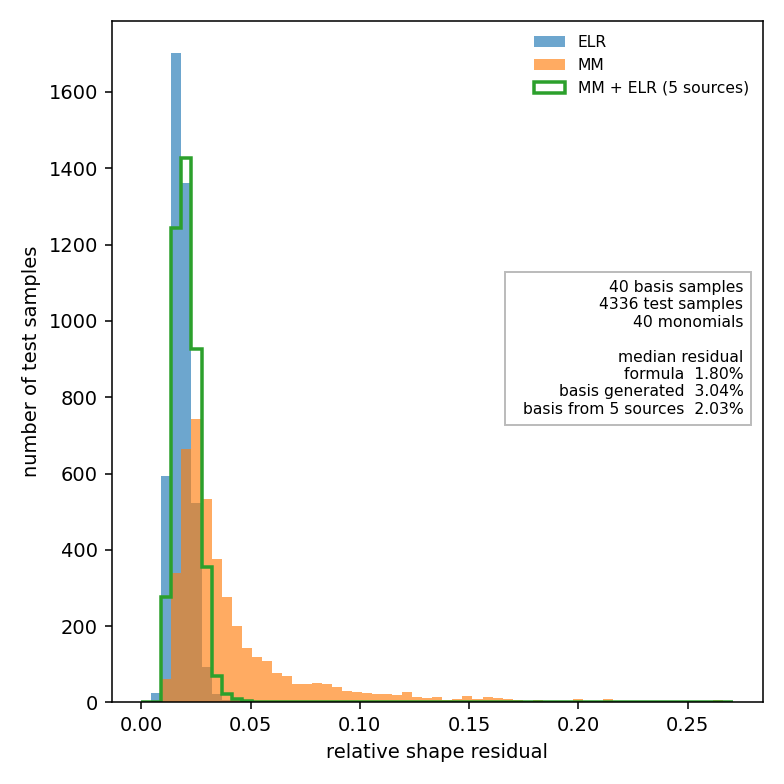
\includegraphics[width=0.48\textwidth]
        {figures/basis_optimization/closure_decomposition_9d.png}
    \caption{Distribution of the relative shape residual, medians quoted in the panel. The distributions correspond to the same median values shown in Figure \ref{fig:basis_shapes}.}
\label{fig:closure_9d}
\end{figure}


\subsection{Closure of the matrix method}
\label{sec:validation_mm}

\begin{figure}[htbp]
    \centering
    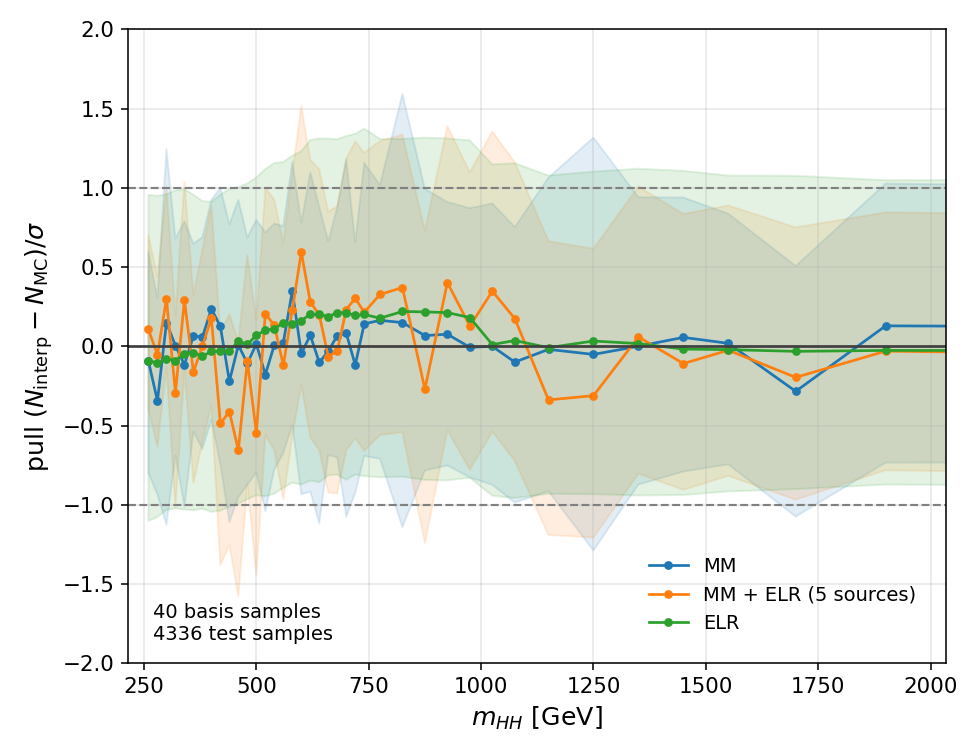
\includegraphics[width=0.62\textwidth]
        {figures/basis_optimization/per_bin_pull_9d.png}
    \caption{Pull per \mHH bin,
    $(N_\mathrm{interp}-N_\mathrm{MC})/\sqrt{\sigma^2_\mathrm{method}+\sigma^2_\mathrm{stat}}$,
    for the matrix method on the basis as generated (MM), with its templates
    built by reweighting from the six sources (MM+ELR), and for the
    $A$-coefficients evaluated directly. Points are the median over the $4336$
    samples and bands the central $68\%$ confidence level. An unbiased prediction has its
    median on zero. A correctly estimated uncertainty gives a band reaching
    $\pm1$, marked by the dashed lines.}
    \label{fig:per_bin}
\end{figure}
\begin{figure}[htbp]
    \centering
    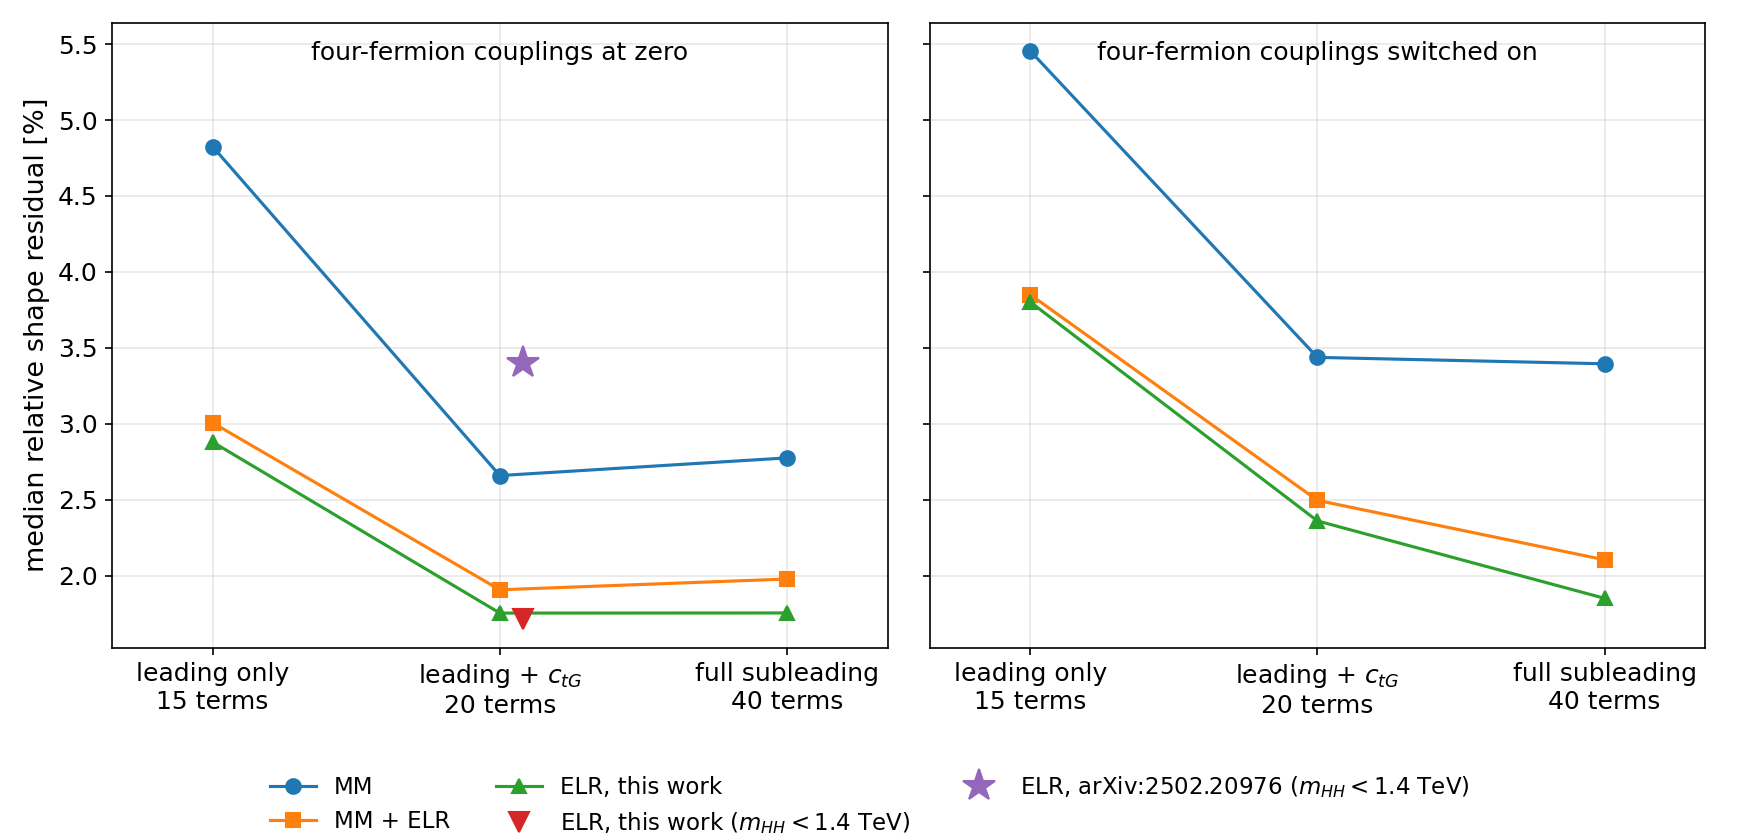
\includegraphics[width=0.96\textwidth]
    {figures/basis_optimization/ladder_comparison.png}
    \caption{Median relative shape residual against the generated samples for three
parameterizations of increasing operators coverage, evaluated on the same $4376$ samples. The panels
separate the samples with the four-fermion coefficients at zero (left) from those with at
least one switched on (right). In the latter case, the leading-only and leading+$c_{tG}$ parameterizations neglect the effects of the four-fermion operators as they are by construction insensitive to them.}
\label{fig:ladder}
\end{figure}

In order to further assess the accuracy found with the recommended BPs, one can look at the pull distributions and investigate how close they are from a Gaussian-like behavior. It can be noticed from Figure \ref{fig:per_bin} that all the distributions fluctuates around zero for the whole $m_\HH$ spectrum. Each point corresponds to the median value over all samples, except for the BPs. All distributions sits well within the $\pm1\sigma$ bands, showing reasonable agreement with an unbiased modeling. 

Additionally, we investigate the results obtained with BPs found for different operators coverage, as described in Figure \ref{fig:ladder}. In particular, for the case restricted to the leading plus chromomagnetic operators, the results can be compared to the ones found with other $A$-coefficients available in the literature \cite{Cadamuro:2025car}\footnote{The coefficients derived in this reference goes only up to $m_\HH=1.4$ TeV. Therefore, for a fair comparison,  the red marker in Figure \ref{fig:ladder} is given by our coefficients evaluated on the same range.} that cover the same set of operators. Given the observed values for the median relative shape residual, a systematic improvement can be observed in all cases (MM, MM+ELR and the $A$-coefficients of this work). Leading-only and leading+$c_{tG}$ parameterizations neglect the additional terms related to the four-fermion operators, and the effect of this is an increase of $\sim1\%$ in the shape residual in the right-side panel regarding the entries for 15 and 20 terms, meaning that in general the four-fermion operators produce very subtle changes in the shapes.

ADD FINAL COMMENTS ABOUT OTHER BASES AND THE FINAL RECOMMENDED ONE.

%The optimized bases reproduce their own parameterization exactly: interpolating the
%$A$-coefficients themselves rather than the simulated yields returns them to a relative
%$10^{-15}$. The residual against the simulated samples is therefore not interpolation
%error. It has two contributions, which can be separated because the reweighting of
%Sec.~\ref{sec:extraction} describes the same cross section independently: the accuracy of
%the parameterization itself, and the Monte Carlo statistics of the basis samples
%amplified by the interpolation weights. For the nominal basis the first is $1.8\%$ and
%the total $3.0\%$ in median relative shape residual, so most of what the matrix method
%adds is the statistical error of its forty samples rather than a failure to describe the
%physics. The pull is close to a standard normal and slightly narrower --- $74.7\%$ of
%entries within $1\sigma$ and $97.1\%$ within $2\sigma$, against $68.3\%$ and $95.4\%$ ---
%so the quoted interpolation uncertainty covers the observed scatter and is conservative
%by about a quarter.

%The left panel of Fig.~\ref{fig:closure_9d} shows the distribution of the residual over
%the test samples for the three cases. What separates the medians of the reweighting and
%the matrix method is not a shift of one narrow distribution relative to another: the
%cores largely overlap, and the difference is a tail of test samples extending beyond
%$10\%$ where the reweighting stops below $5\%$. That is the signature of a statistical
%effect concentrated on the samples whose prediction leans on the least populated
%templates. Building the basis templates by reweighting from five sources removes the tail
%and returns the median to $2.03\%$, against $1.80\%$ for the reweighting itself and
%$3.04\%$ for the basis as generated.

%One alternative explanation can be excluded directly. If the excess came from a minority
%of test points that the interpolation reaches only through large, cancelling weights, it
%would track the size of those weights. It does not: correlating the residual with
%$\sum_i|w_i|$ over the test set gives $-0.10$ for the matrix method, and the comparison
%with the reweighting is unchanged at every weight norm, the right panel of
%Fig.~\ref{fig:closure_9d}. The excess is a property of the precision of the forty
%templates as a set, which is why improving those templates removes it everywhere rather
%than only in the badly conditioned corners.

%\begin{figure}[htbp]
%    \centering
%    \includegraphics[width=0.48\textwidth]
%        {figures/basis_optimization/closure_decomposition_9d.png}
%    \includegraphics[width=0.48\textwidth]
%        {figures/basis_optimization/residual_vs_weight_9d.png}
%    \caption{Closure of the nominal nine-coefficient basis over the $4336$ generated samples
%that are not themselves basis points, for the reweighting fit evaluated directly (ELR),
%the matrix method on the basis as generated (MM), and the matrix method with every basis
%template built by reweighting from five generated samples (MM\,+\,ELR). Left:
%distribution of the relative shape residual, medians quoted in the panel. Right: the same
%residual against the summed magnitude of the interpolation weights, with the correlation
%quoted in the panel.}
%\label{fig:closure_9d}
%\end{figure}

\label{sec:validation_perbin}
%Those quantities are medians over the whole \mHH range. Resolved bin by bin the relative
%residual rises by a factor $6.1$ between the threshold region and $2$~TeV for the matrix
%method. Dividing by the uncertainty that should account for it, Fig.~\ref{fig:per_bin}
%shows the pull $(N_\mathrm{interp}-N_\mathrm{MC})/\sigma$ with
%$\sigma^2=\sigma^2_\mathrm{method}+\sigma^2_\mathrm{stat}$, combining the statistical
%error of the test sample with the propagated uncertainty of the prediction. Those differ
%between the three: the matrix method on generated templates carries the statistics of its
%forty basis samples, the same method on reweighted templates the smaller uncertainty of
%an inverse-variance combination, and the reweighting evaluated directly neither.

%The median tests for bias and sits at zero for all three across the spectrum, $+0.01$,
%$+0.03$ and $+0.03$ overall. The width tests the uncertainty, and the $68\%$ bands span
%$[-0.81,+0.87]$, $[-0.75,+0.89]$ and $[-0.93,+1.11]$ against the $\pm1$ of a correctly
%estimated error: the reweighting is calibrated and the two matrix-method cases are
%slightly narrow. The rise of the unnormalized residual with \mHH is accounted for by the
%growth of these two statistical errors, the test samples having three orders of magnitude
%less yield in the last bin than in the first.

%The bin-to-bin wander of the median is larger for the reweighted templates than for the
%generated ones, $0.28$ against $0.13$. The quantities behind the two numbers set that in
%context. The reweighted case has the smaller absolute residual, $2.03\%$ against
%$3.04\%$, and its worst test sample closes at $5\%$ where the generated basis reaches
%$70\%$. What the pull divides by is smaller still: the uncertainty of an inverse-variance
%combination is $0.55$ times the statistical error of a test sample, where the generated
%basis gives $1.51$, so the same deviation in cross section is displayed about three times
%larger. One contribution to the extra wander is that the five sources are reweighted with
%the same fitted coefficients and so are not strictly independent, which the
%inverse-variance combination assumes; the per-bin weighting removes most of that.


%The medians conceal a difference between the methods. The distribution of the residual
%over the test samples has a long tail for the matrix method on generated templates and
%a short one for the other two: the $99$th percentile is $23.8\%$ and the worst
%single sample reaches $70\%$, against maxima of $5.1\%$ and $5.2\%$ for the reweighted
%templates and the reweighting itself. The tail is not an artefact of a few pathological
%samples --- removing the worst $5\%$ moves the median only from $3.04\%$ to $2.95\%$.

%The $70$ samples with a residual above $20\%$, $1.6\%$ of the test set, have a median
%cross section of $23$~fb against $240$~fb for the test set as a whole, and the rank
%correlation between cross section and residual is $-0.74$. These are the points where the
%contributions cancel and the rate is small, so a given absolute error is a large relative
%one; the diagonal ridge of Fig.~\ref{fig:closure_9d} is the same feature seen in a
%coupling plane. The pull does not show a tail there, so the interpolation uncertainty
%already covers it. Building the basis templates by reweighting removes the tail: the
%median goes from $3.04\%$ to $2.03\%$ and the worst case from $70\%$ to $5\%$.

%\subsection{Effect of increasing dimensionality on the fit}
%\label{sec:validation_ladder}

%Adding coefficients to the parameterization adds terms to be solved for and samples to be
%simulated. Scoring every parameterization on the same samples --- the full
%nine-coefficient set, rather than each on the region where it happens to be exact ---
%measures what each step up buys. With the four-fermion coefficients at zero the
%twenty-term parameterization is already exact and the forty-term one adds nothing, both
%at $1.8\%$: the extra twenty terms describe operators that are switched off. With the
%four-fermion coefficients switched on the forty-term parameterization is the only one
%that keeps improving, $1.9\%$ against $2.4\%$. The gain is the recovery of a sector the
%smaller parameterizations cannot represent at all, which is the behaviour found for the
%ladder of Ref.~\cite{HH_nonggf_R5}.

%The published coefficients of Ref.~\cite{ELR_topdipole} are compared only where they are
%defined. Their fit stops at $m_{HH}=1.4$~TeV, so both they and our own twenty-term
%coefficients are evaluated on exactly the bins below it, and neither is favoured by the
%range. Extending them naively over the full range instead --- holding the last fitted bin
%constant in density, which is what an analysis using that formula at high mass would be
%forced to assume --- gives $13.15\%$ against the $3.40\%$ obtained where the fit is
%defined, with five of the forty bins extrapolated. That number measures the extrapolation
%and not the fit, which is why it is quoted here rather than drawn.

%Fig.~\ref{fig:ladder} shows three curves. The reweighting curve is the parameterization
%alone and improves monotonically along the ladder, $3.80$, $2.36$, $1.85\%$ with the
%four-fermion coefficients switched on. The matrix-method curve adds the statistical error
%of the basis samples, which is why it improves much less over the last rung, $3.44$ to
%$3.40\%$: forty basis samples carry more statistical error than twenty, and that almost
%exactly cancels the gain from the richer description. Building the basis templates by
%reweighting separates the two effects and recovers it, $2.50$ to $2.11\%$. The ordering
%of the underlying parameterizations is therefore visible only once the basis statistics
%are removed. The cost of the extra dimensionality is paid in sample statistics rather
%than in the description, and it is a cost the reweighting removes.

%All three are evaluated on the same $4376$ samples, so a parameterization that omits
%operators pays for it here rather than being scored only where it is exact. The
%improvement with the size of the parameterization is confined to the right panel: with
%the four-fermion coefficients at zero, the twenty-term description is already exact.


\clearpage
\section{A realistic analysis scenario}
\label{sec:validation_realistic}

Everything up to this point has been measured on the generated samples with no selection
applied. An analysis sees instead the events that survive a trigger, a reconstruction and
a set of cuts, in one corner of phase space that the basis optimization knew nothing
about, as raw LHE kinematics was used at that step. This section applies the method in the signal region of $\HH\to\bbbar\bbbar$, using the public
release of Ref.~\cite{CMS:2026znu,hepdata.171917}, and measures the performance of the developed tools in realistic phase spaces.

The release provides generator-level trees with the two Higgs boson four-vectors and the
event weight, for both resolved and a fully merged topologies, at four values of
$\kappa_\lambda$---therefore outside SMEFT parameter space. Since the trees carry \mHH, $\cos\theta^*$ and
$\pt^{\HH}$ event by event, the ELR can use them as an input to the multi-ref approach to produce templates at any point of the SMEFT parameter space, before or after the selection. With this procedure we generate all the BPs after the SR selection.

In order to explore the MM coverage of the full 9D parameter space in the SR, one can investigate the acceptance times efficiency provided by each topology by doing 1D scans for each of the Wilson coefficients, and then comparing the smooth interpolation given by the MM with the outcome obtained with the ELR evaluated in a few points of the scan. Figure~\ref{fig:acc_4b} shows how the selection efficiency varies as a function of each of the relevant Wilson coefficients, hinting which corners of the parameter space are favored according to each topology. This is then summarized on Table \ref{tab:acceptance_response}, which shows how each topology responds to variations in each Wilson coefficient. It can be noticed that the boosted selection zooms in on the coefficients that populate the high-mass tail (e.g., $c_{\text{HG}}$ and $c_{u\text{H}}$), while in the resolved case, a larger portion of the kinematic phase space is selected and the topology averages over different structures, therefore not strongly favoring some coefficients over others. Additionally, the impact of the chromomagnetic operator is similar to that of the leading operators, while the four-fermion operators indeed exhibit subtle changes in the acceptance, with $c^{(1)}_{\text{Qt}}$ and $c^{(8)}_{\text{Qt}}$ being nearly degenerated, and $c^{(8)}_{\text{QQ}}$ the least impactful.

It must be noticed that an operator may change the cross section by a large factor and the acceptance not at all, meaning that the information extracted from Figure \ref{fig:acc_4b} and Table \ref{tab:acceptance_response} must be complemented with a notion about how the overall cross section behaves in the parameter space---It does not really matter if, for instance, the boosted topology has 100\% selection efficiency in a corner of the parameter space where the overall cross section is orders of magnitude smaller than in regions where the same selection has an acceptance times efficiency of 10\%.





%The quantity throughout is the acceptance times efficiency, the template integral over
%the cross section, in which the luminosity and the next-to-next-to-leading-order factor
%cancel. Fig.~\ref{fig:acc_4b} shows it against each Wilson coefficient in turn, the other
%eight held at zero, for both selections.

%The curves of Fig.~\ref{fig:acc_4b} are built from the basis templates, which the
%reweighting itself produced. The reweighting therefore appears on both sides of them and
%the basis points are reproduced by construction, so on their own the curves establish
%that the interpolation is smooth, not that it is right. The test is to apply the
%reweighting directly: the same events are reweighted to a point that is not in the basis,
%the same selection is applied, and the integral is compared with what the matrix method
%predicts there from the forty templates. Fifty-two such points were produced, eight or
%nine along each of the six coefficients of Fig.~\ref{fig:acc_4b} and over the full range
%of each, in both selections: the open circles of that figure. Every one of them agrees
%with the matrix method to better than $0.1\%$. Each point carries the
%statistical error of the reweighted template combined with that of the reweighting
%coefficients, and the error bars are smaller than the markers almost everywhere.

%Those deviations are smaller than the uncertainty of the templates themselves at every
%point, which the same figure shows as bands. The accuracy quoted in
%Sec.~\ref{sec:validation_mm} without a selection therefore survives one, in both
%selections and along every coefficient the selections respond to. Both selections agree
%at a level set by numerical precision rather than by any property of the phase space:
%once the two sides use the same reweighting, the same input treatment and the same
%binning, the matrix method reproduces the reweighting. This is a statement that the
%morphing is algebraically faithful to the parameterization it is built on, not that
%either description of the high-mass tail has been verified against simulation there. The
%only point in this section that tests more than that is the SM, where a directly
%generated sample exists and is compared with the reweighted prediction; the closure of
%the methods against samples they were not built from is the subject of
%Sec.~\ref{sec:validation_mm}.

%Comparing the matrix method against the reweighting over a plane would need the
%reweighting evaluated directly on a grid of points rather than along a line, which is a
%large amount of computation for a figure whose conclusion a one-dimensional scan already
%carries. The verification here is therefore one-dimensional throughout. The planes that
%do appear below ask which operators matter in a selected phase space rather than whether
%the interpolation is faithful, and they cost only evaluations of the model.

\begin{figure}[htbp]
    \centering
    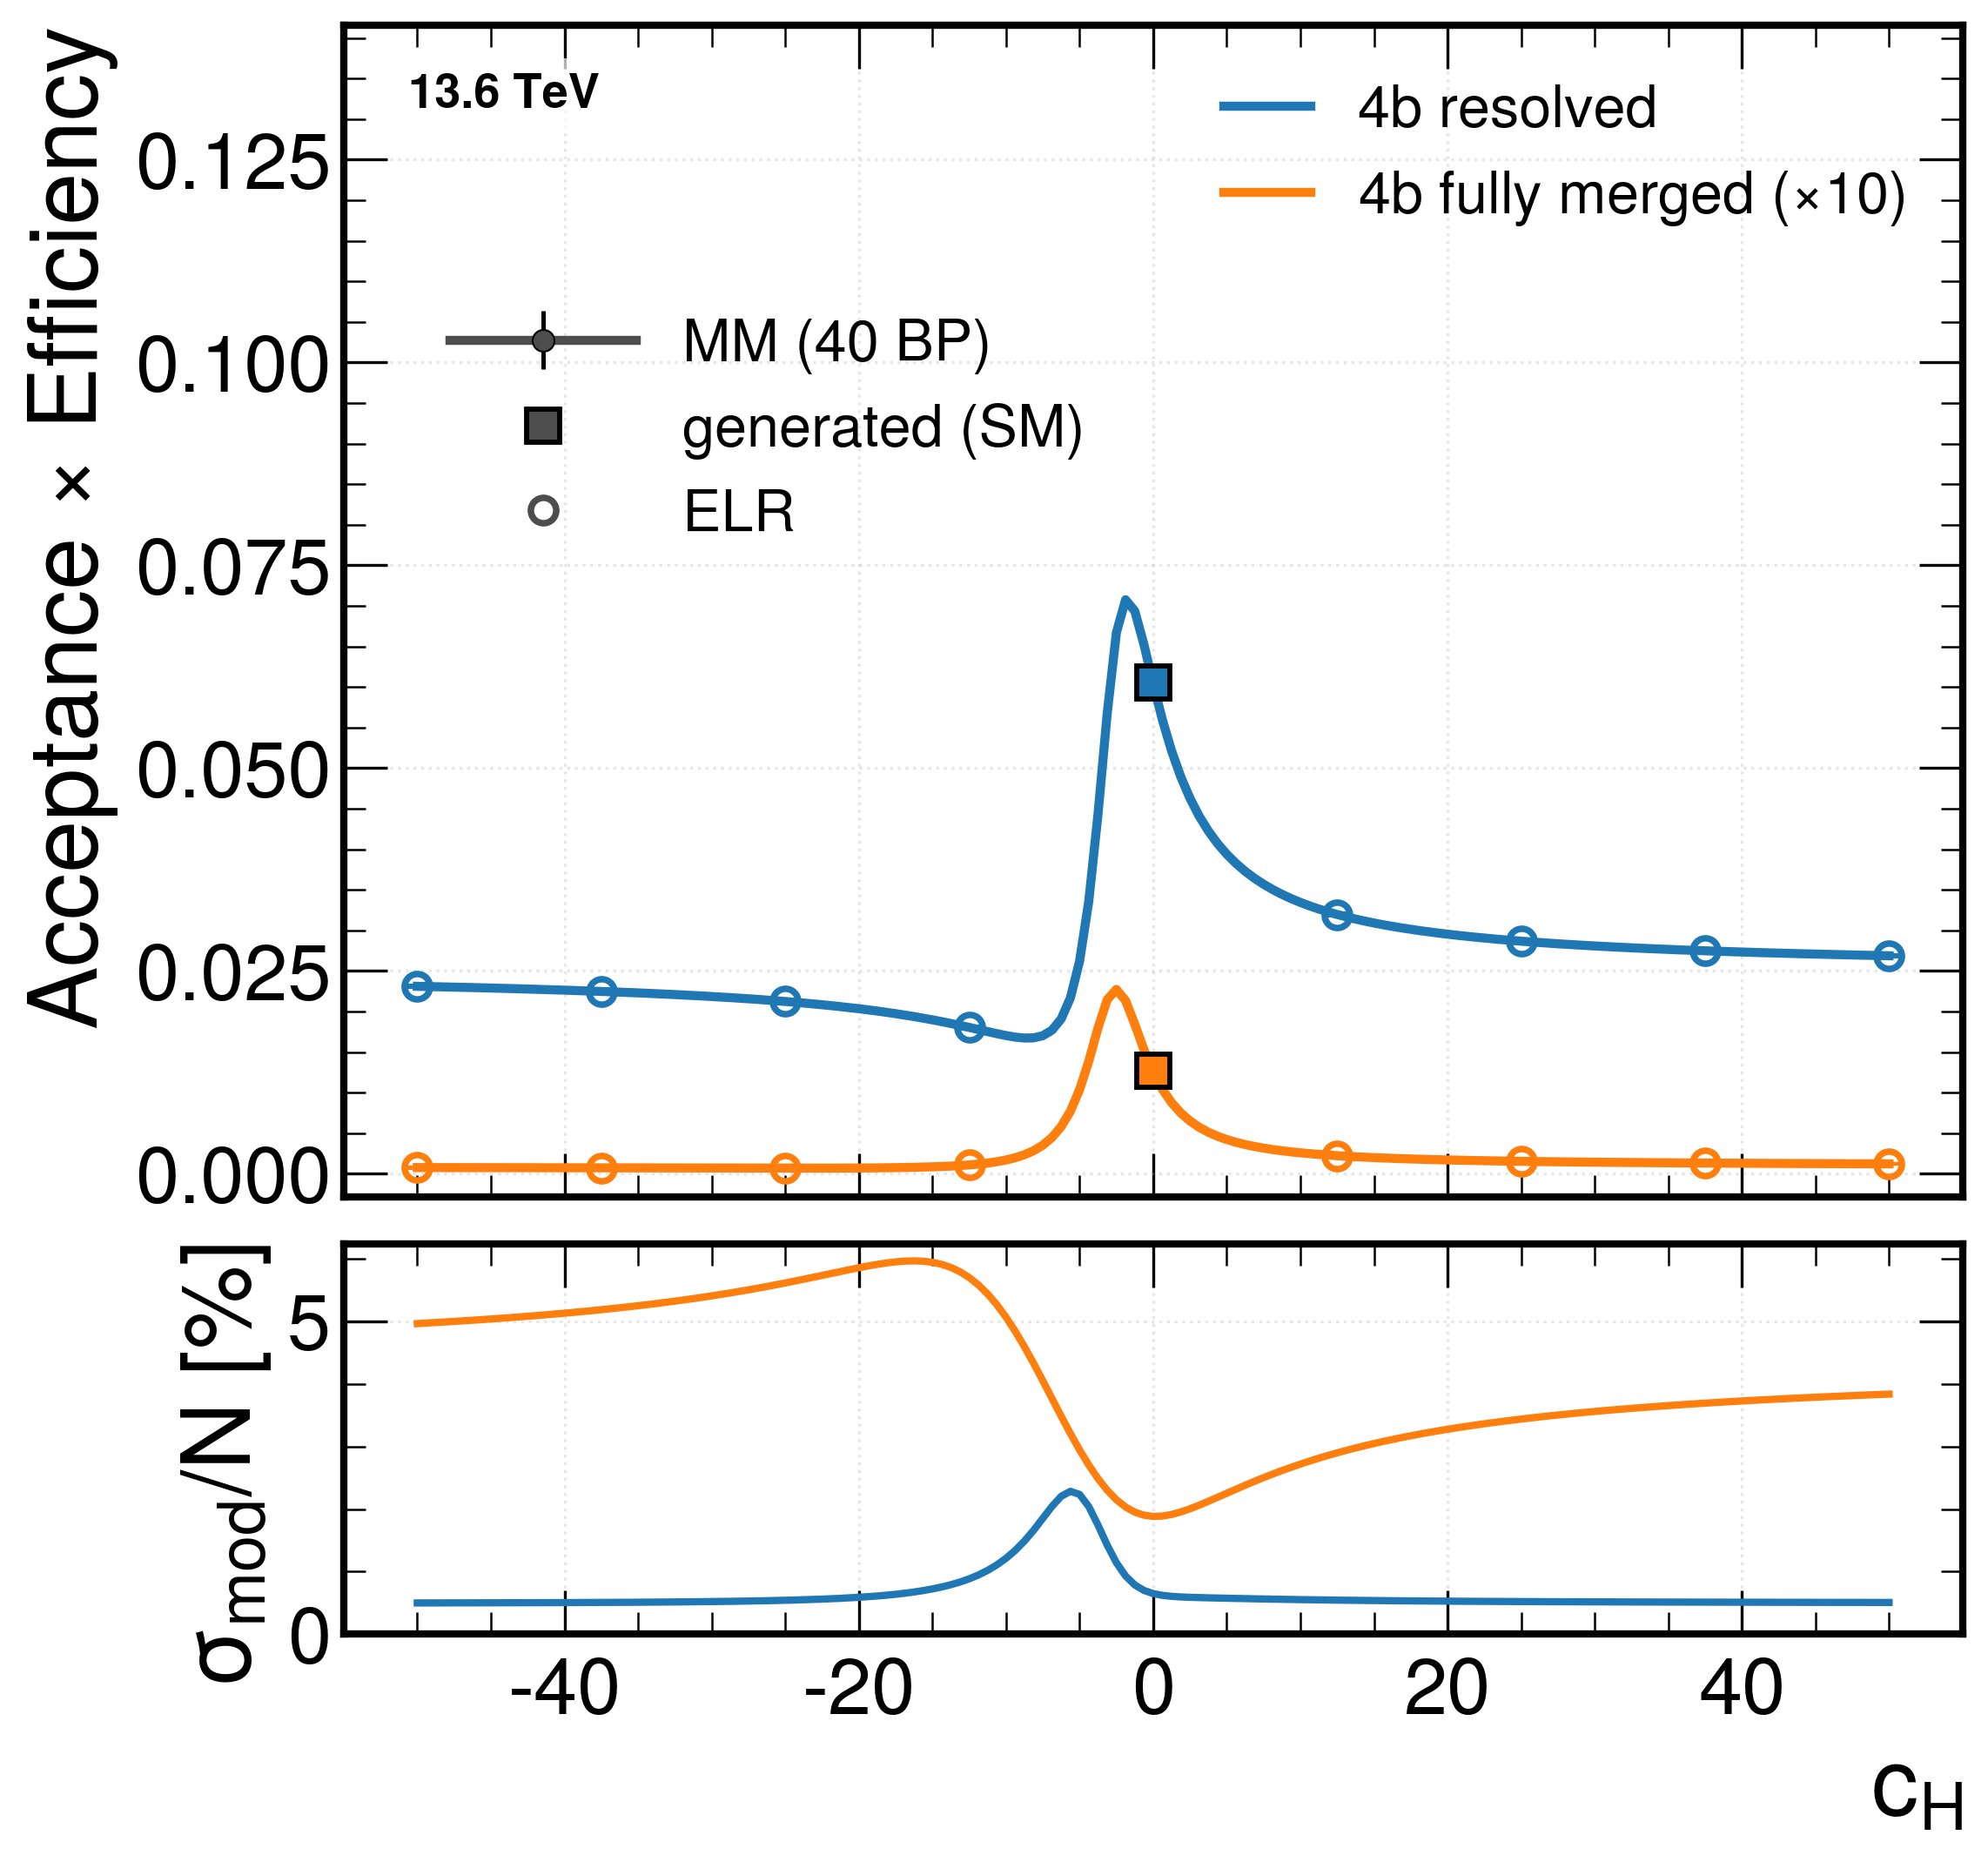
\includegraphics[width=0.32\textwidth]{figures/basis_optimization/eff4b_cH.png}
    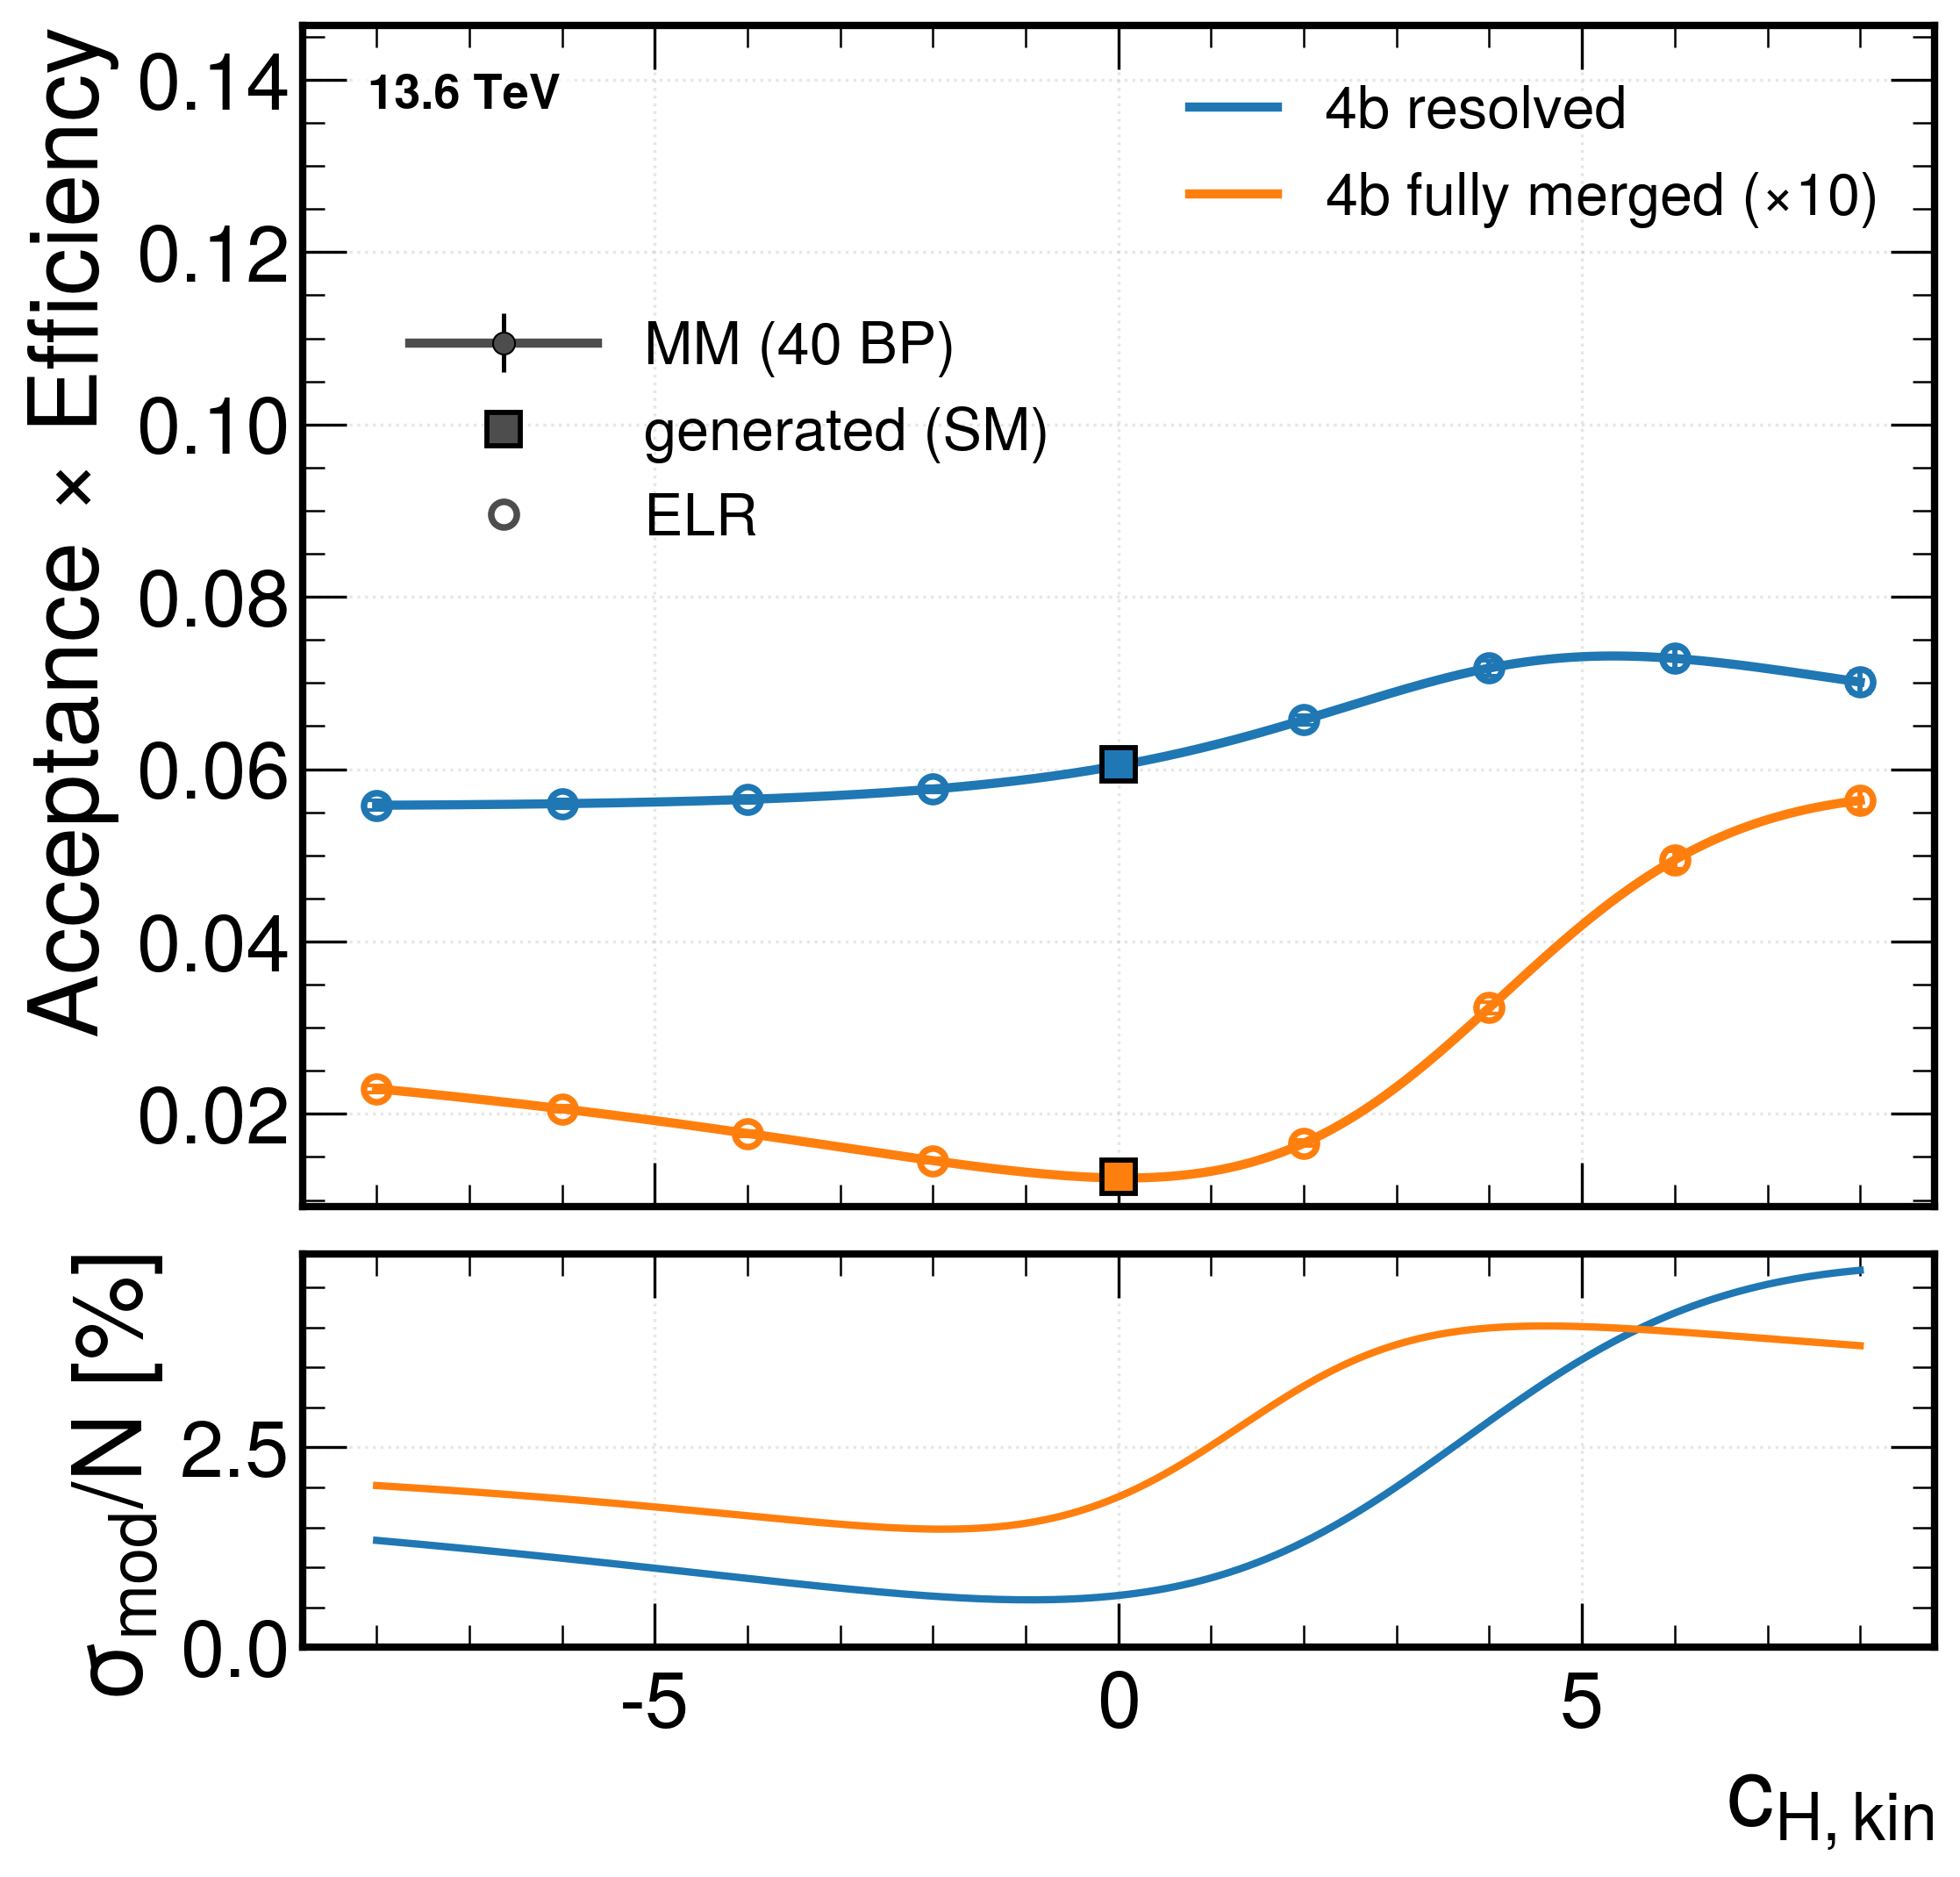
\includegraphics[width=0.32\textwidth]{figures/basis_optimization/eff4b_cHkin.png}
    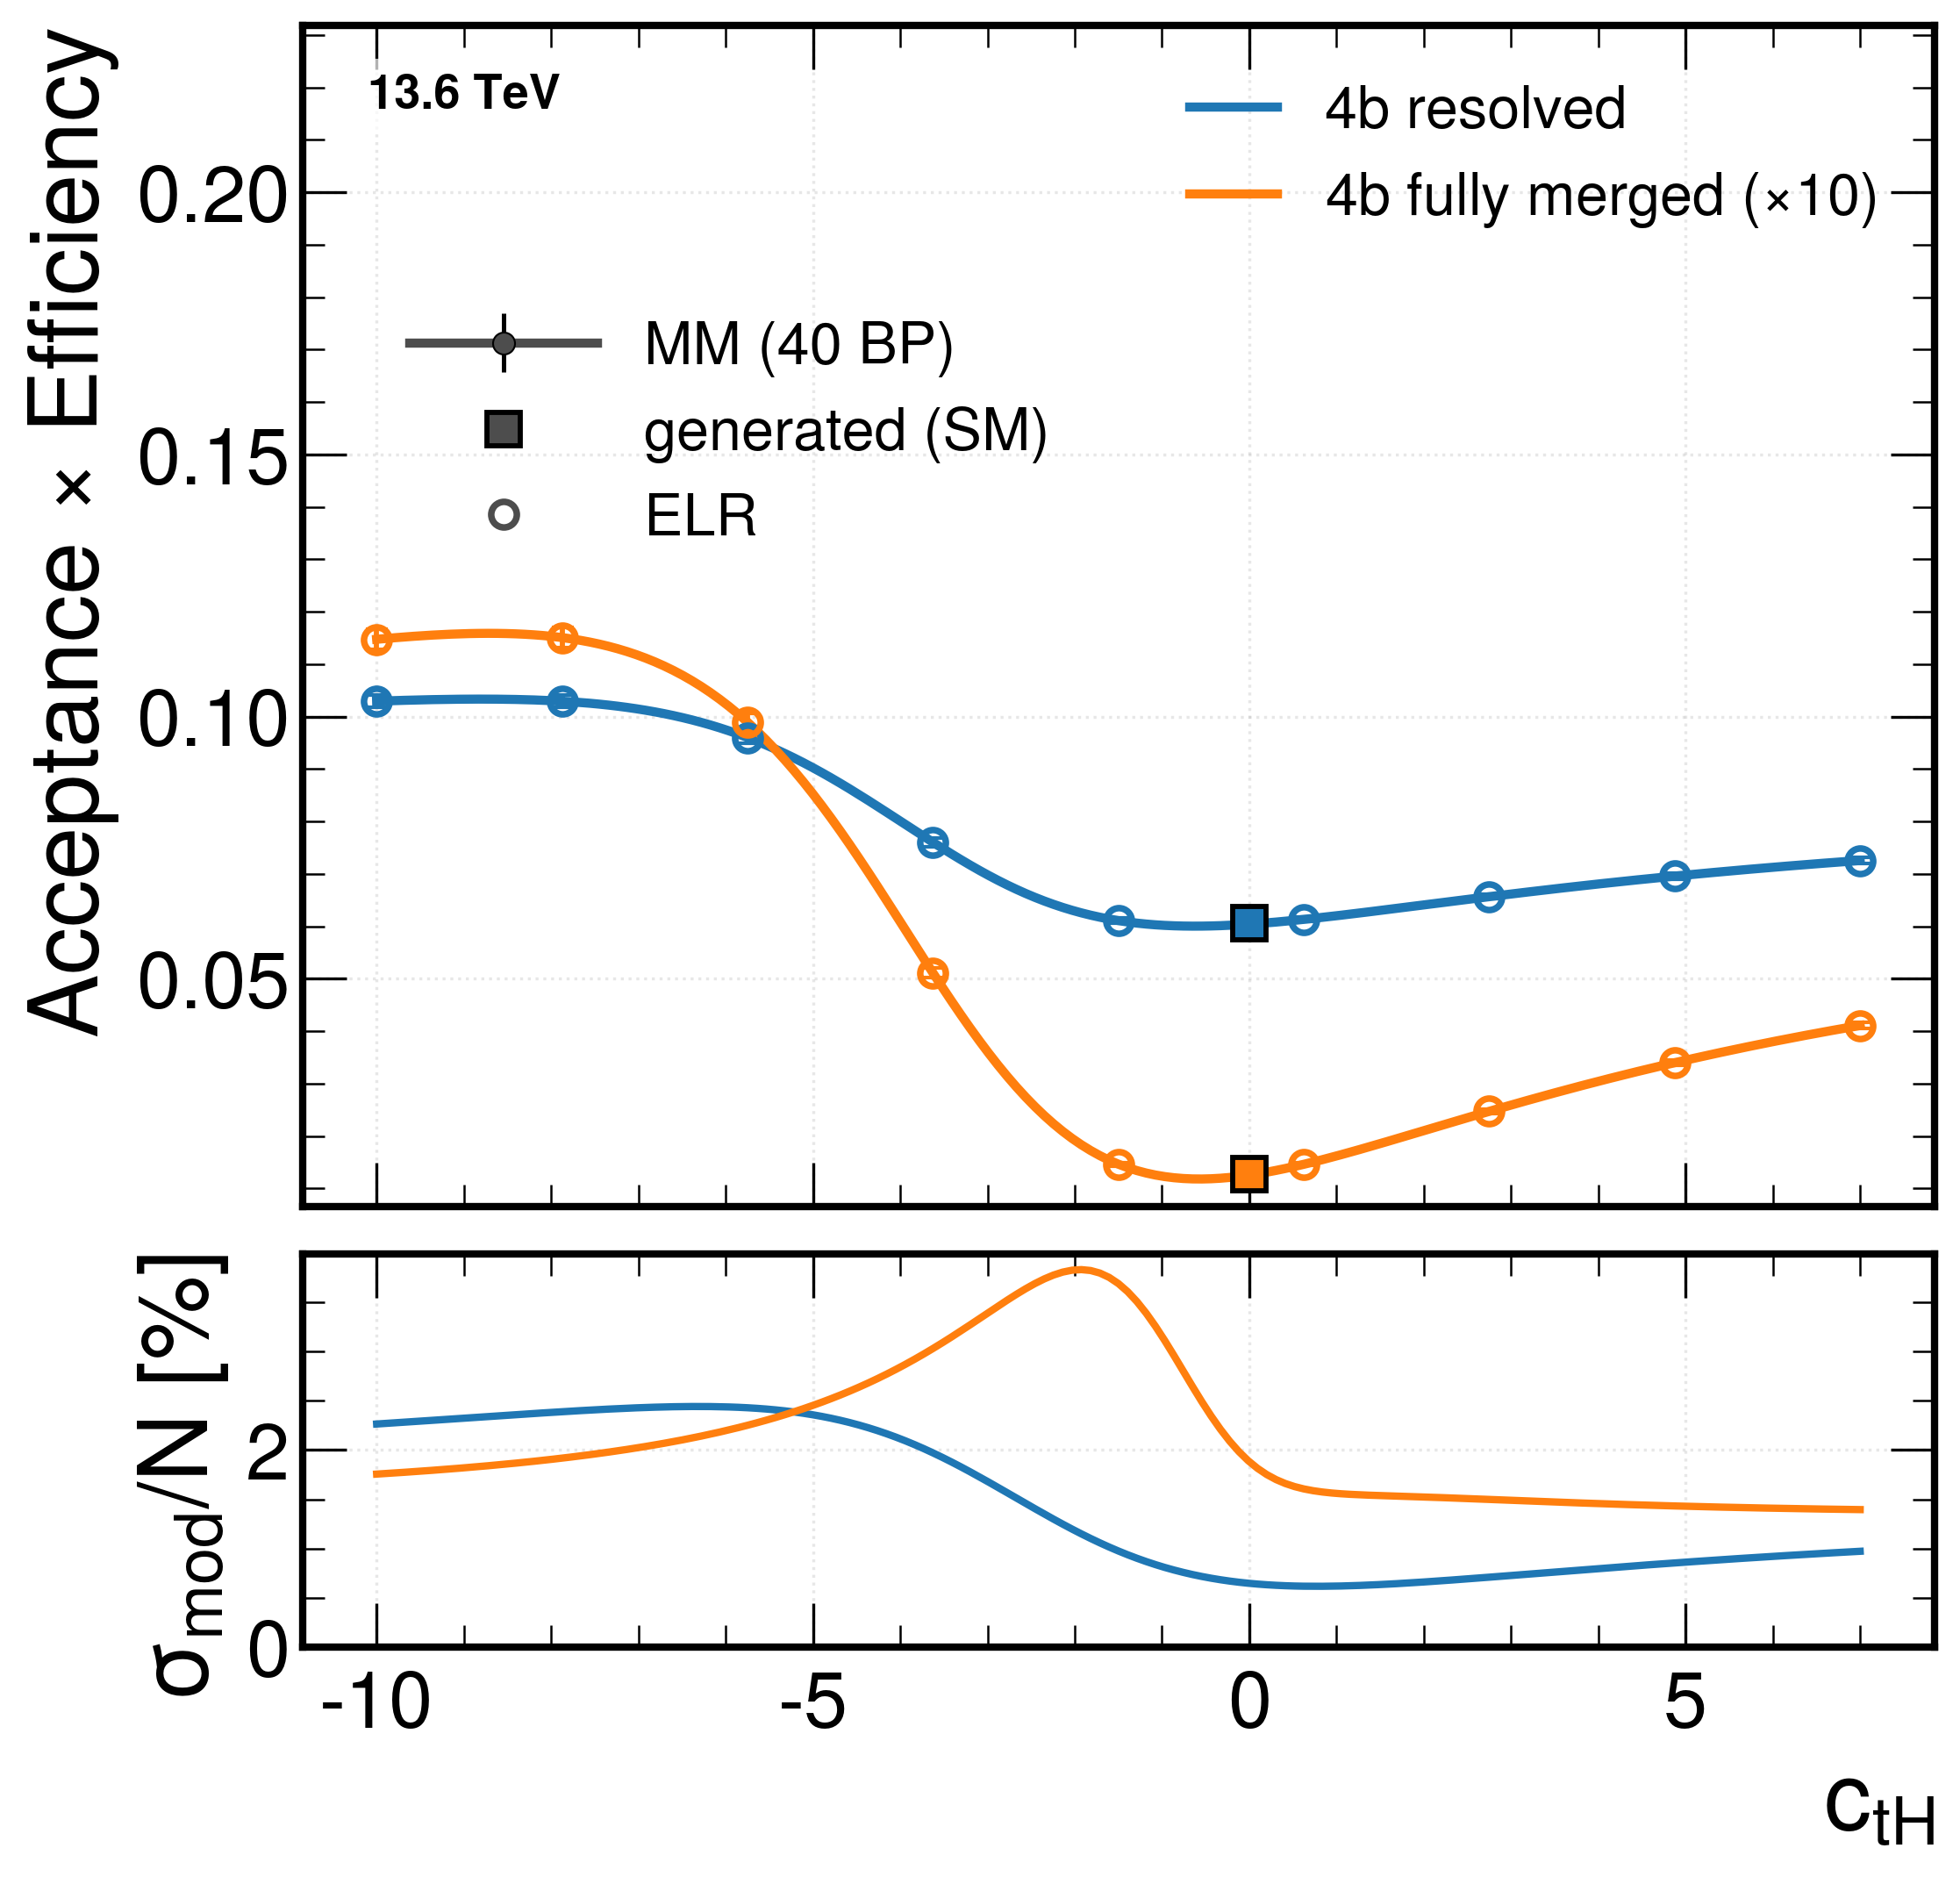
\includegraphics[width=0.32\textwidth]{figures/basis_optimization/eff4b_ctH.png} \\
    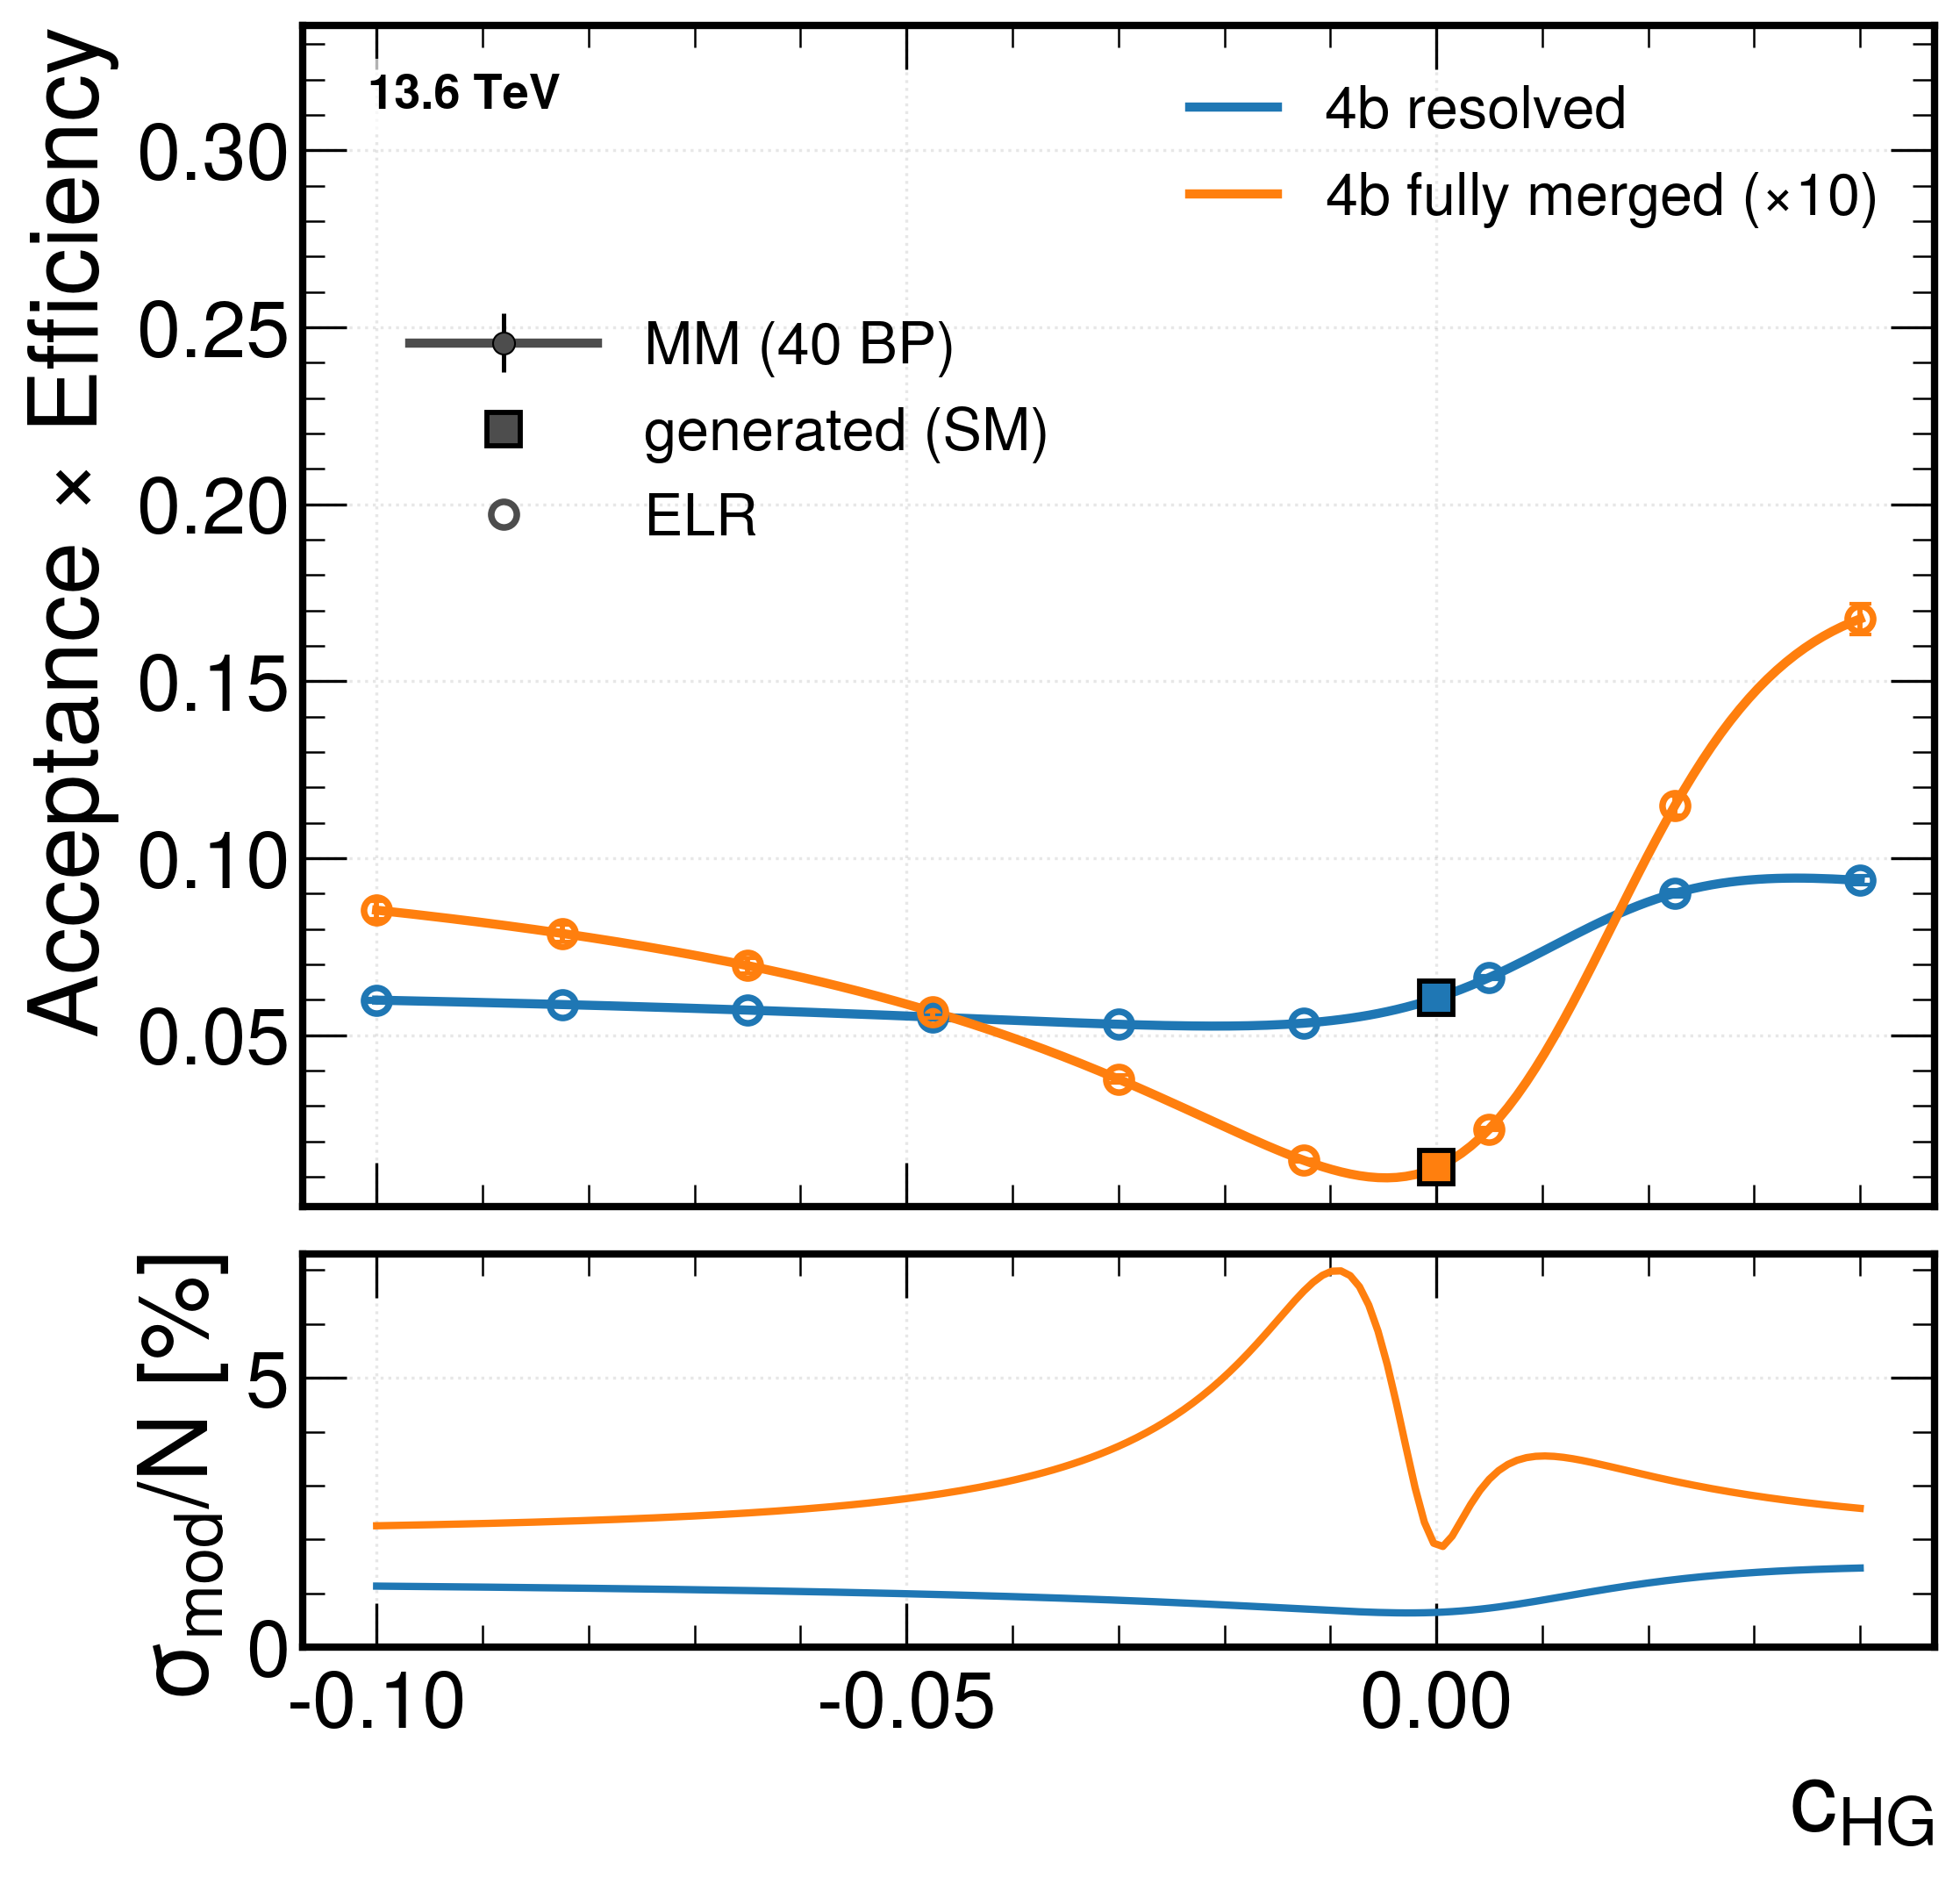
\includegraphics[width=0.32\textwidth]{figures/basis_optimization/eff4b_cHG.png} 
    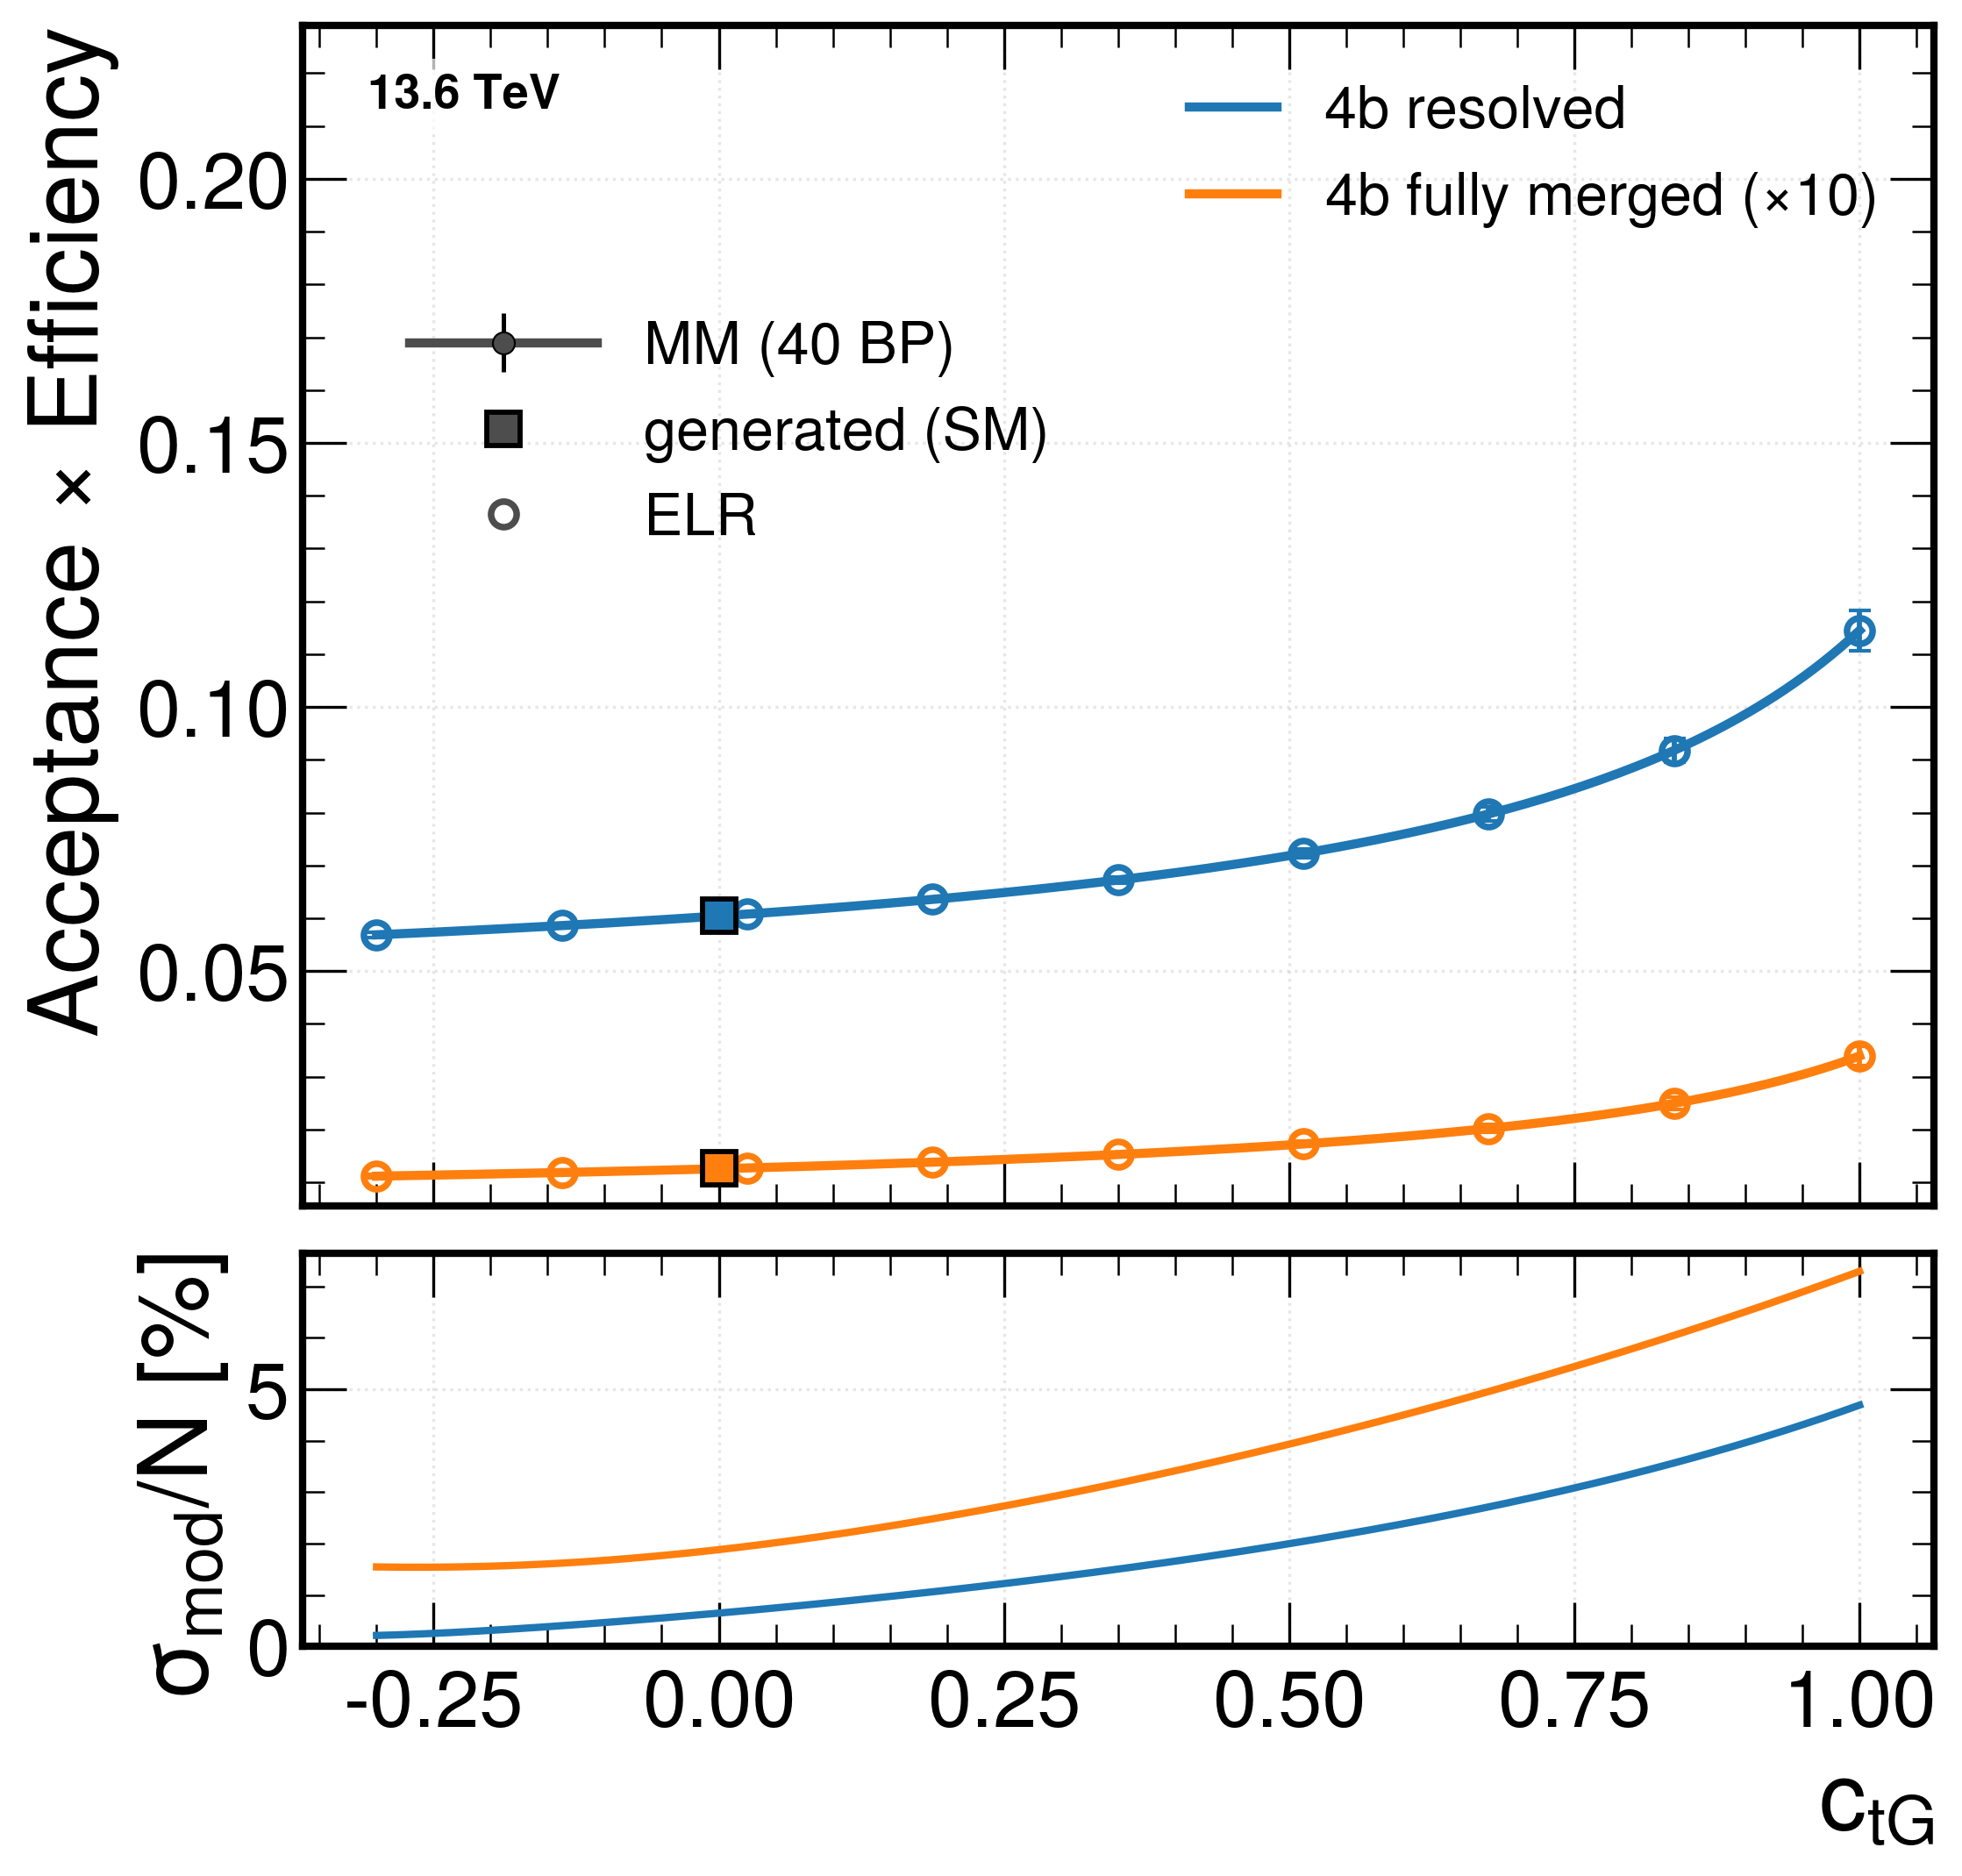
\includegraphics[width=0.32\textwidth]{figures/basis_optimization/eff4b_ctG.png}%
    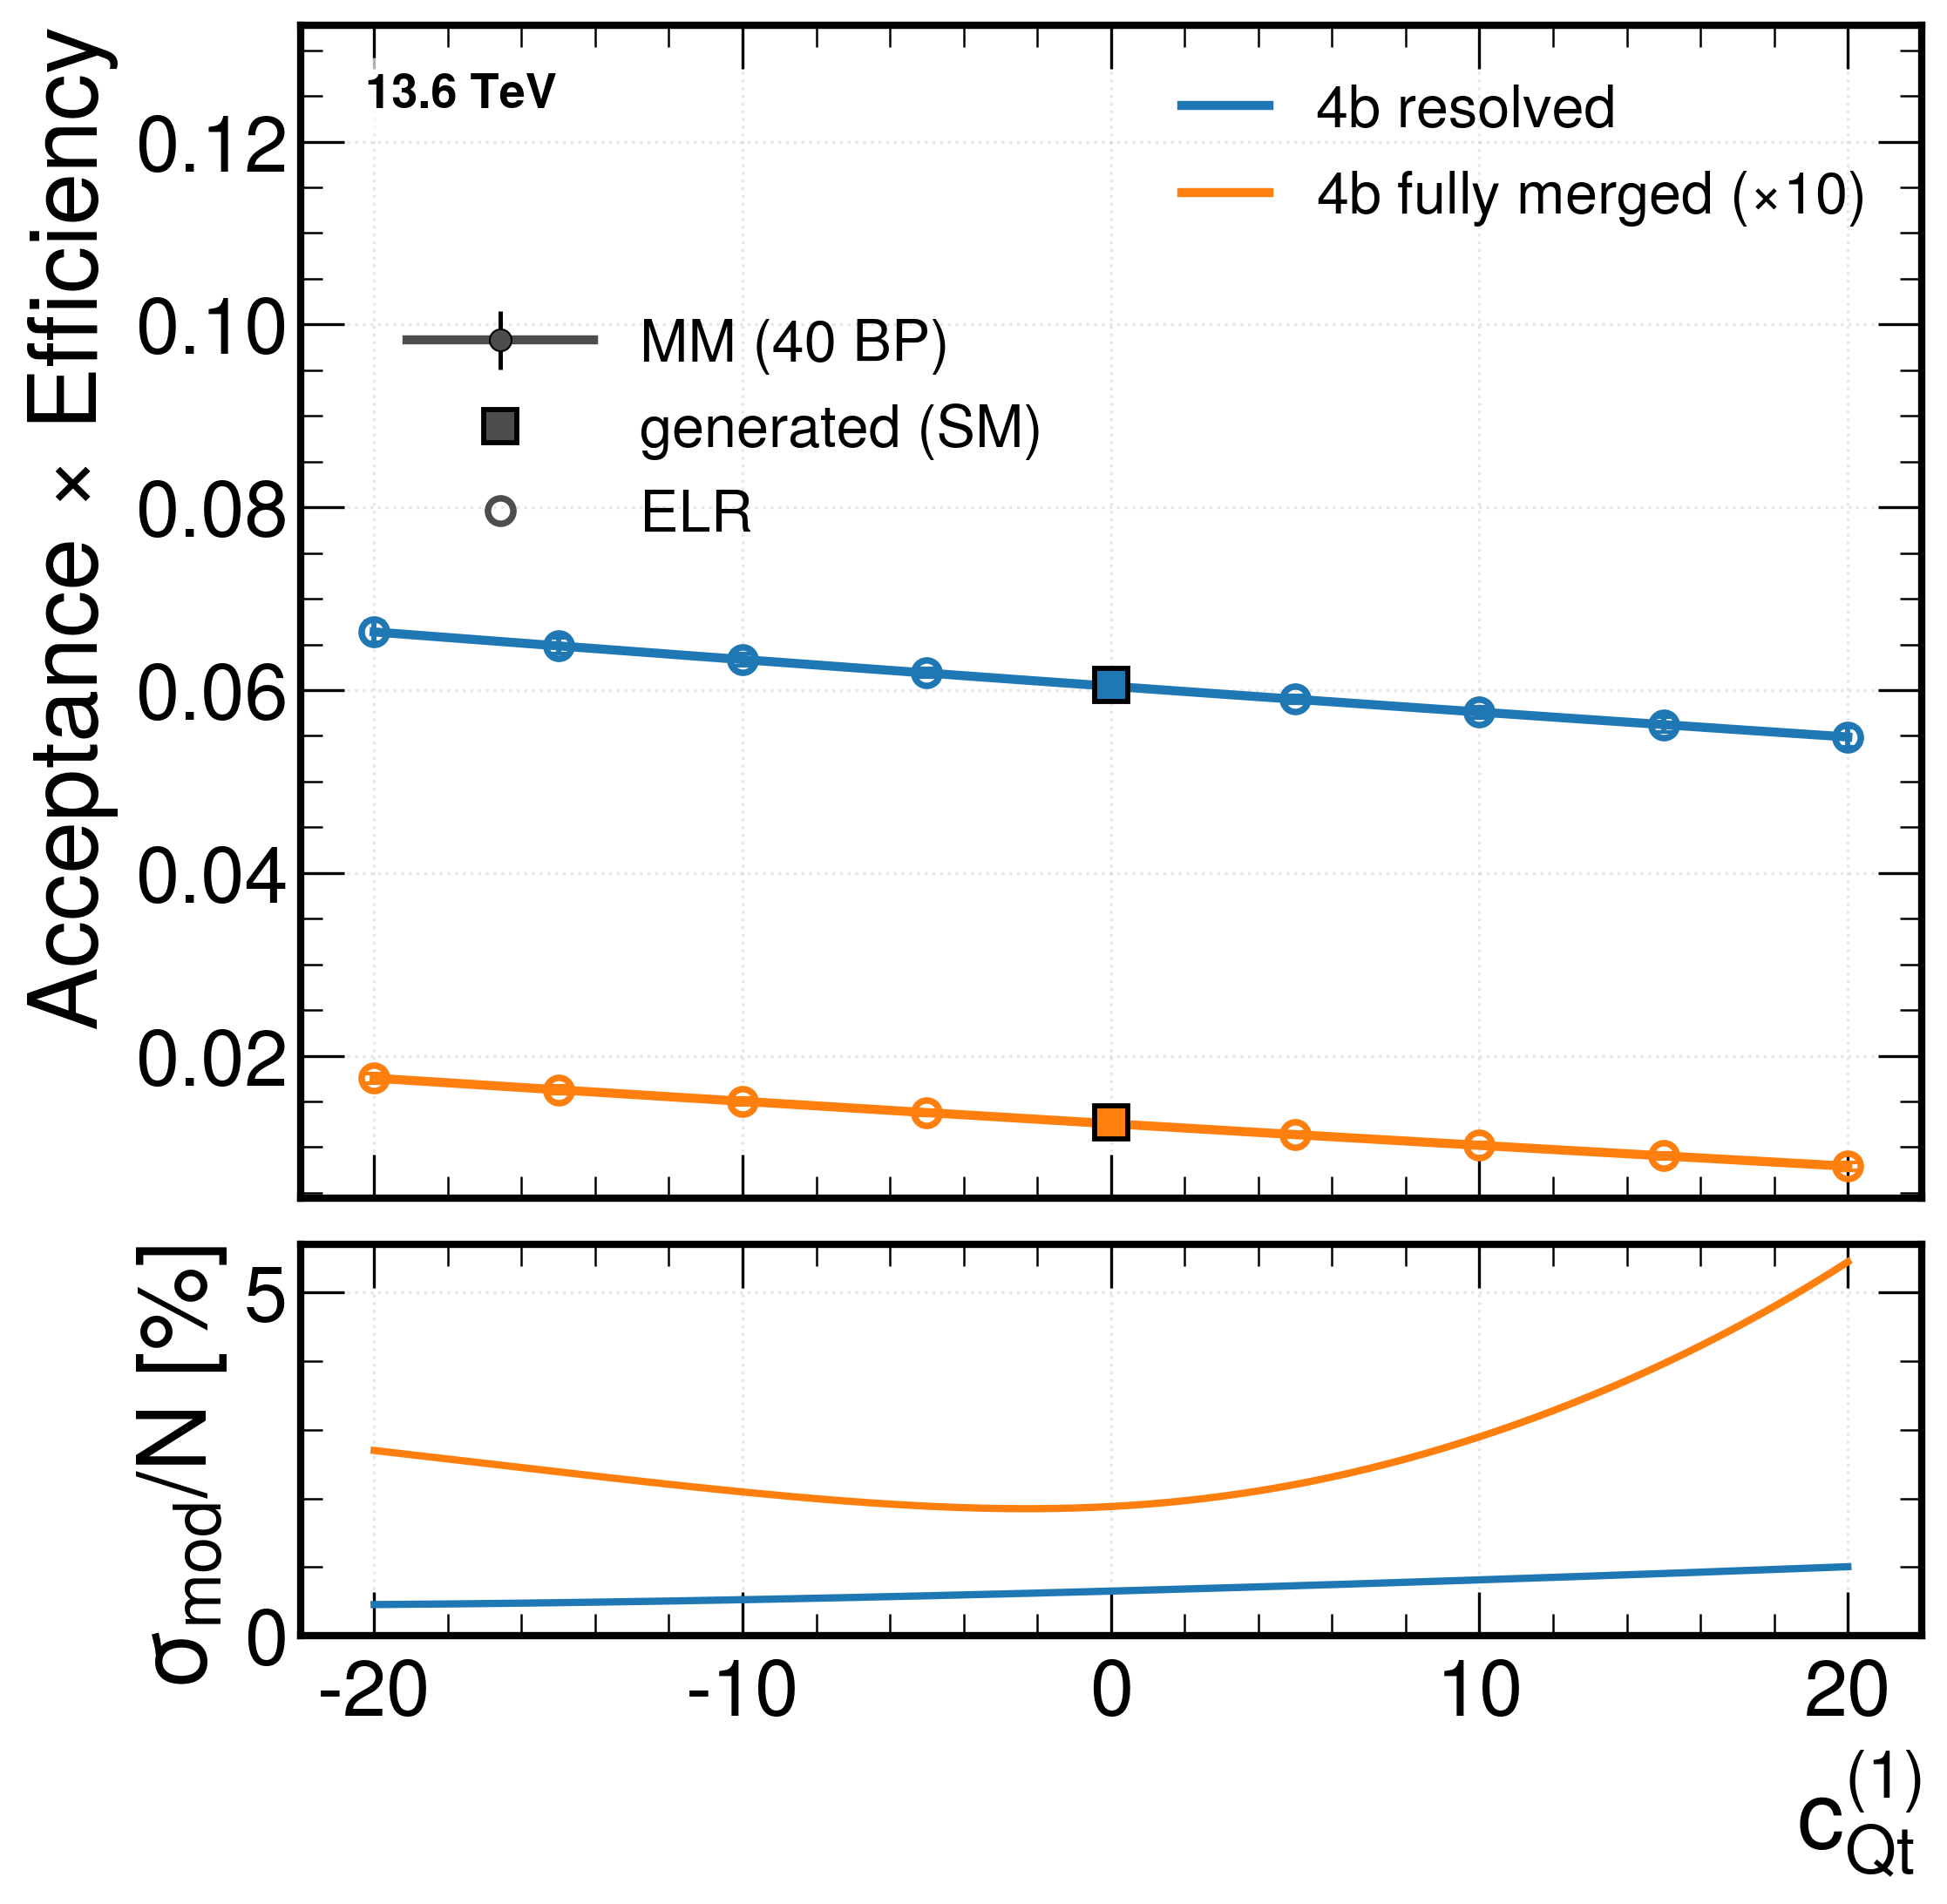
\includegraphics[width=0.32\textwidth]{figures/basis_optimization/eff4b_cQt1.png}
    \caption{Acceptance times efficiency against each Wilson coefficient, the other eight
held at zero, for the resolved and fully merged selections of Ref.~\cite{CMS:2026znu}. The merged curve is
multiplied by ten. Blue and yellow curves: the matrix method on the optimized basis, with bands combining
the statistical error of the templates and the uncertainty of the reweighting
coefficients. Open circles: the ELR applied directly on the corresponding points. Filled square: the directly generated $\kappa_\lambda=1$
sample (SM). Three coefficients are omitted: $c_{Q\PQt}^{(8)}$, $c_{QQ\PQt\PQt}$, and $c_{QQ}^{(8)}$, which have small response in both topologies.}
\label{fig:acc_4b}
\end{figure}
\begin{table}[htbp]
\centering
\begin{tabular}{l|cccc|ccccc}
\hline
 & \multicolumn{4}{c|}{leading} & \multicolumn{5}{c}{subleading} \\
 & $c_{\PH}$ & $c_{\PH\mathrm{kin}}$ & $c_{\PQt\PH}$ & $c_{\PH G}$ & $c_{\PQt G}$
 & $c_{Q\PQt}^{(1)}$ & $c_{Q\PQt}^{(8)}$ & $c_{QQ\PQt\PQt}$ & $c_{QQ}^{(8)}$ \\
\hline
4b resolved      & $0.79$ & $0.37$ & $0.96$ & $0.90$ & $1.03$ & $0.19$ & $0.17$ & $0.02$ & $0.00$ \\
4b merged  & $1.8$  & $3.6$  & $8.6$  & $13.2$ & $1.8$  & $0.78$ & $0.91$ & $0.09$ & $0.03$ \\
\hline
\end{tabular}
\caption{Relative spread over the scanned
range of each coefficient. This is obtained by computing the $(\max-\min)$ acceptance times efficiency divided by the value obtained at the SM value,
with the other eight coefficients held at zero. %The ranges are those of
%Table~\ref{tab:SMEFTcouplings}. $c_{\PQt G}$ is listed with the leading
%coefficients here because it behaves like them.}
}
\label{tab:acceptance_response}
\end{table}

%This setting also answers whether a separate, smaller basis is worth building for a
%linearly truncated interpretation. A ten-point basis for the interference-only prediction
%exists (Appendix~\ref{sec:appendix_linear}) and would cost ten simulated samples instead
%of forty. Applied to these two selections it does not work: four of its ten templates
%have a negative yield in the fully merged selection, and one, at $c_{\PQt\PH}=-10$ and
%$c_{\PH G}=-0.0567$, is negative in every region while its inclusive cross section stays
%positive, so it can enter a fit neither as a shape nor as a rate. The positivity imposed
%during the basis search acts on the inclusive total, and inclusive positivity does not
%survive a selection that favours the high-mass tail, which is where the truncated
%prediction is most negative. A basis search cannot repair this in advance because it does
%not know the selection.

%What fails is the saving, not the linear truncation. A linearly truncated prediction
%remains available from the forty-point basis: its templates are untruncated physical
%distributions, and the linear prediction is formed at evaluation by restricting the
%forty-coefficient solve to the ten linear monomials $A_0$--$A_4$ and $A_{15}$--$A_{19}$,
%which reproduces samples generated with the same truncation
%(Appendix~\ref{sec:appendix_linear}). No template is negative in that route, because no
%template is itself a truncated object; the truncated \emph{prediction} can still turn
%negative at large couplings, but that is the expansion leaving its validity window
%(Appendix~\ref{sec:appendix_trunc_validity}) rather than a defect of the basis. The cost
%is forty samples rather than ten, and the two bases are not interchangeable. An analysis
%restricting its coupling ranges may not meet the problem at all, since every negative
%point lies far from the SM. The measurements behind this are in
%Appendix~\ref{sec:appendix_linear_selection}.

\subsection{Which operators a selected phase space is sensitive to}
\label{sec:validation_subleading_role}

%Which Wilson coefficients change what an analysis measures is a property of the selection
%as much as of the operators, and the two selections of the $\HH\to\bbbar\bbbar$ release
%differ sharply enough to compare. The quantity is again the acceptance times efficiency,
%evaluated from the basis alone: it needs no simulation beyond the templates already made,
%and being a ratio it is insensitive to anything that scales the rate uniformly. An
%operator may change the cross section by a large factor and the acceptance not at all.




%Table~\ref{tab:acceptance_response} gives the response and Fig.~\ref{fig:acc_4b} shows
%it. Three things follow. The merged selection is more responsive than the resolved one by
%an order of magnitude for the coefficients it responds to at all: its acceptance is
%$0.11\%$ against $4.15\%$ at the SM, and it varies by a factor thirteen across the range
%of $c_{\PH G}$ where the resolved selection varies by a factor two. A selection keeping
%only the most boosted events is sensitive to the operators that populate the hard tail;
%the resolved selection, keeping most of the spectrum, averages over that structure.

%The ordering also changes between the two. In the resolved selection $c_{\PQt G}$ gives
%the largest response and $c_{\PH G}$ the third; in the merged one $c_{\PH G}$ dominates
%and $c_{\PQt G}$ falls to fifth. Which operator an analysis is most sensitive to is
%therefore not a property of the operator alone, and a statement of the form ``this
%analysis constrains $c_{\PH G}$ best'' is a statement about its selection.

%The four-fermion sector splits into two pairs. $c_{Q\PQt}^{(1)}$ and $c_{Q\PQt}^{(8)}$
%move the acceptance, $0.8$ to $0.9$ in the merged selection and comparable to $c_{\PH}$
%there, though below $0.2$ in the resolved one. $c_{QQ\PQt\PQt}$ and $c_{QQ}^{(8)}$ are
%consistent with no response, a spread of $0.00$ to $0.09$: neither selection separates
%the SM from the edge of the scanned range.

%Within each pair the two members are nearly degenerate, which bears on what a fit can
%separate. Normalizing each response to its SM value and comparing over the full range,
%$c_{QQ\PQt\PQt}$ and $c_{QQ}^{(8)}$ differ by $3\%$ and $c_{Q\PQt}^{(1)}$ and
%$c_{Q\PQt}^{(8)}$ by at most $20\%$, the difference confined to the merged selection
%above $c_{Q\PQt}\simeq5$; in the resolved selection they agree to $2\%$ everywhere. The
%two members of each pair are the colour-singlet and colour-octet forms of the same
%operator, so they enter through closely related topologies and differ only by colour
%factors. An analysis using the resolved selection alone cannot distinguish
%$c_{Q\PQt}^{(1)}$ from $c_{Q\PQt}^{(8)}$ by acceptance, however many samples it
%simulates. They do change the cross section, and Sec.~\ref{sec:validation_ladder} showed
%that the parameterization cannot describe the generated samples without them: their
%effect is close to a normalization, so an analysis measuring a rate will constrain them
%while one relying on the selection to separate them will not.

%No selection of this example therefore measures a four-fermion direction: two of them are
%flat and the other two are degenerate with each other. Carrying them in the parameterization buys
%something else. They are needed to describe the generated samples
%wherever they are switched on, which is what Sec.~\ref{sec:validation_ladder} measures,
%so a five-coefficient description fitted to such a region would absorb their effect into
%the coefficients it does have; and they are the coefficients through which the
%renormalization-group running reaches the Higgs operators at all
%(Sec.~\ref{sec:rge}).

A scan through one coefficient holds the others at zero, which hides whatever two of them
do jointly. Fig.~\ref{fig:planes} shows the acceptance
over three planes: the two coefficients the merged selection responds to most strongly,
the pair in which the cross section has its cancellation, and the strongest leading
coefficient against the strongest subleading one. No plane is drawn with $c_{QQ\PQt\PQt}$
or $c_{QQ}^{(8)}$, along which nothing happens, and none with $c_{\PQt G}$ against
$c_{Q\PQt}^{(1)}$, which is vertical banding: the acceptance depends on the first and not
on the second, as the one-dimensional scans already say. These are the only
two-dimensional figures in this report, and they are affordable because the acceptance is
evaluated from the basis: a plane costs model evaluations, not simulation.

Two things about reading the figure. The merged panels are multiplied by ten and each row then
shares one colour scale, so that colours may be compared across a row; without the
scaling the two panels would be coloured on ranges a factor forty apart. And the crosses
are the forty basis points projected on the plane --- their two coordinates in it, the
other seven ignored --- so a cross marks where the basis constrains the surface read
along those axes, not that a template was simulated at that point. Most of the forty have
their two non-zero couplings elsewhere and project onto the axes of the plane.

\begin{figure}[p]
    \centering
    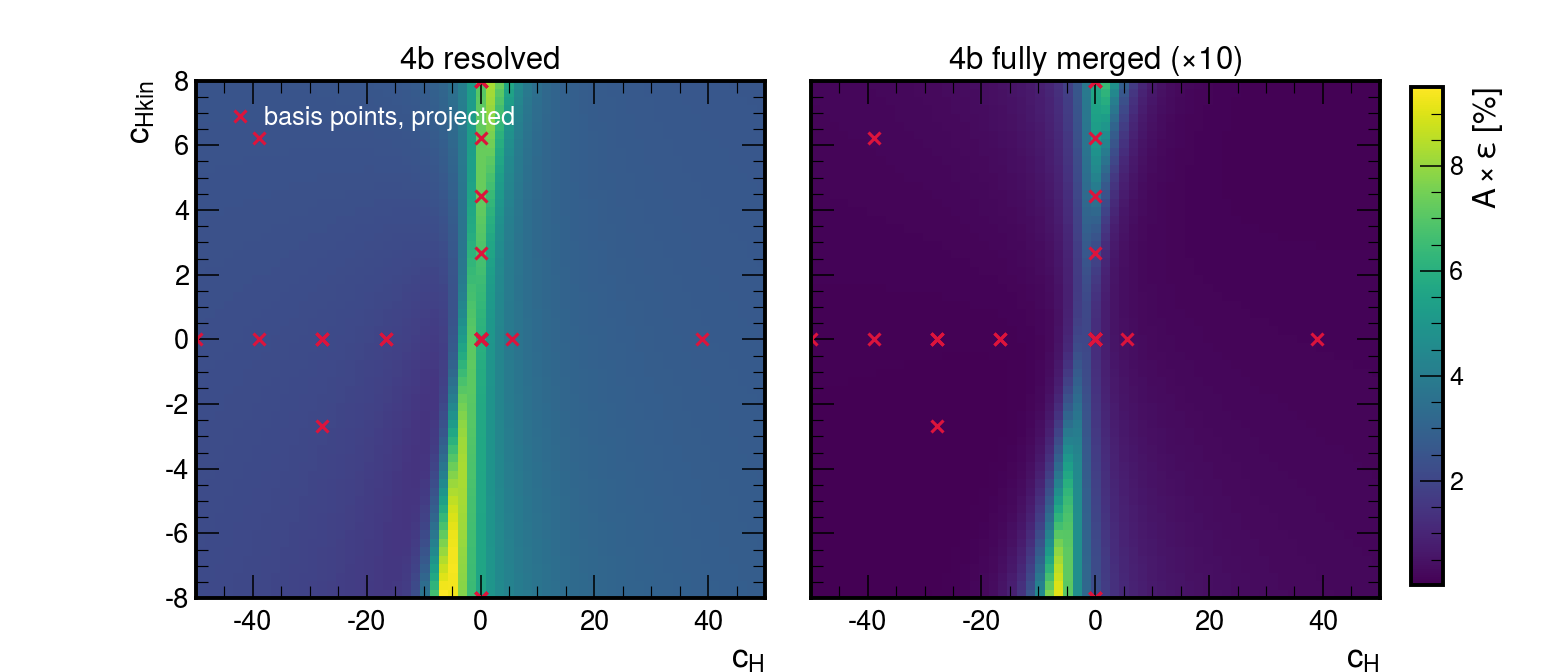
\includegraphics[width=0.88\textwidth]
        {figures/basis_optimization/plane_cH_cHkin.png}\\[4pt]
    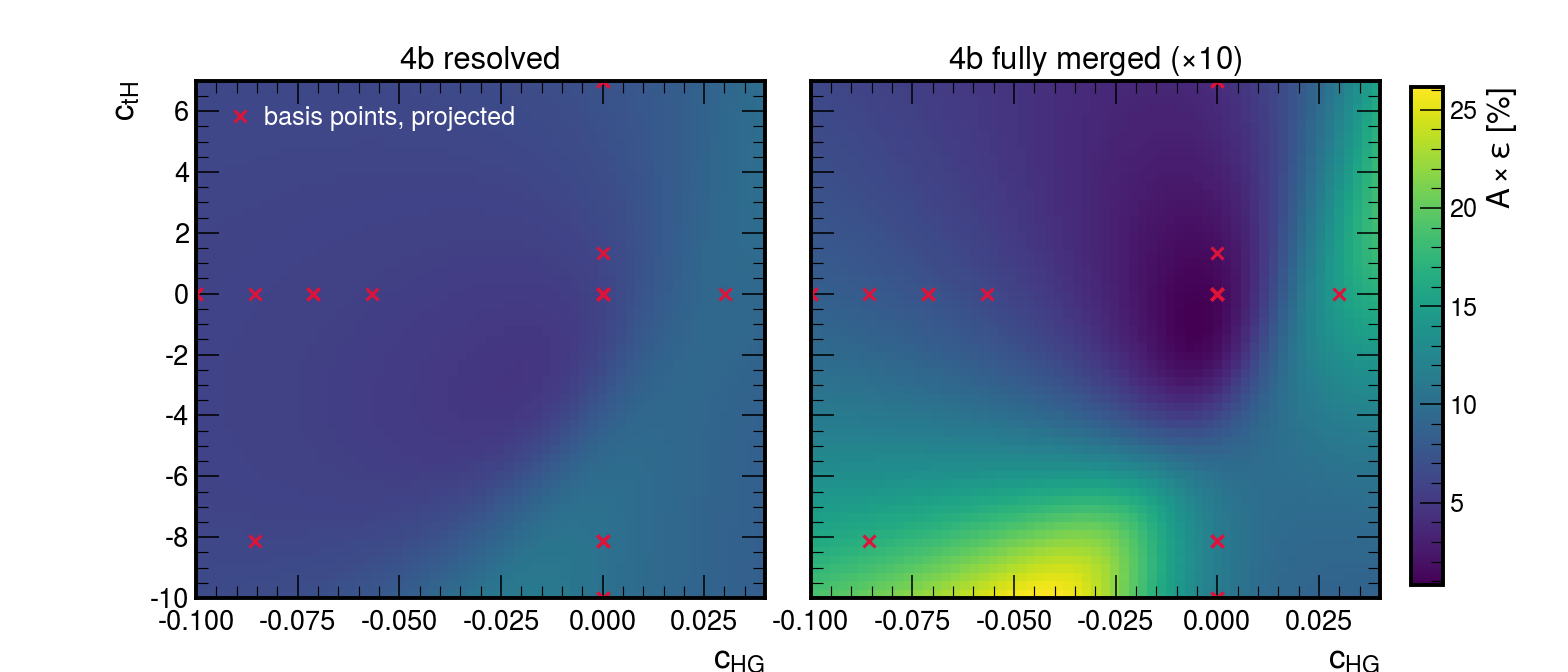
\includegraphics[width=0.88\textwidth]
        {figures/basis_optimization/plane_cHG_ctH.png}\\[4pt]
    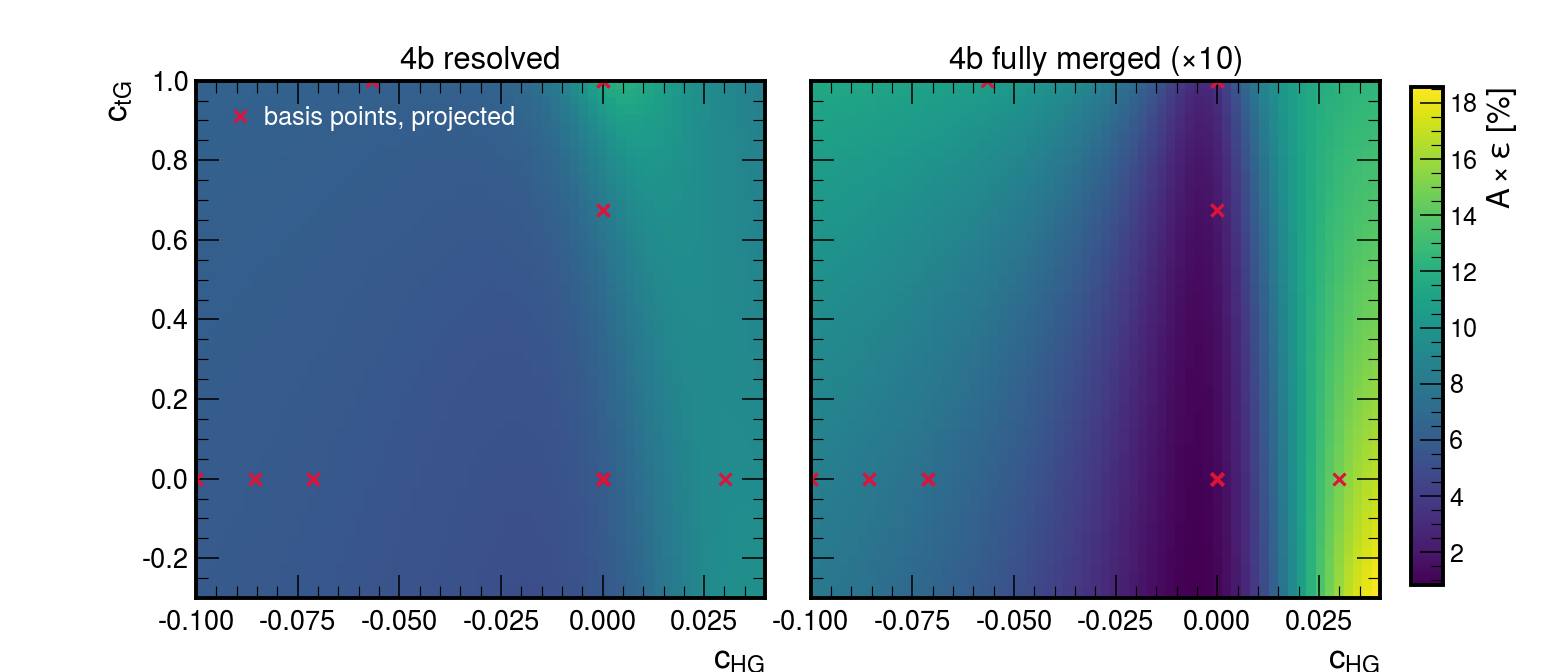
\includegraphics[width=0.88\textwidth]
        {figures/basis_optimization/plane_cHG_ctG.png}
    \caption{Acceptance times efficiency over three coupling planes, the other seven
    coefficients at zero, for the resolved (left) and fully merged (right) selections of
    Ref.~\cite{CMS:2026znu}. From top to bottom:
    $c_\PH\mbox{--}c_{\PH\mathrm{kin}}$, $c_{\PH G}\mbox{--}c_{\PQt\PH}$ and
    $c_{\PH G}\mbox{--}c_{\PQt G}$. Each merged panel is scaled by ten and shares the
    colour range of the resolved one in its row. Crosses are the basis points of
    Table~\ref{tab:smeft_basis_9d} projected on the plane.}
    \label{fig:planes}
\end{figure}

\subsection{The interpolation uncertainty an analysis would quote}
\label{sec:validation_realistic_band}

An analysis that adopts the basis of this report derives nothing about the effective field
theory in order to obtain its interpolation uncertainty. The statistical error of the forty
templates propagates with the same weights the prediction uses,
Eq.~\eqref{eq:sigmainterp}, evaluated independently in every bin; the derivation and its
calibration against the residual observed are in Sec.~\ref{sec:uncertainties}. The weights $w_i(\mathbf{c})$ are a
property of the basis alone: they follow from the parameterization and the forty points,
they are the same in every bin, and they are independent of the selection applied and of
the quantity being histogrammed. They are published once, with the basis. The $\sigma_i$
are the statistical errors of the basis templates as the analysis itself has them, after
its own trigger, reconstruction and selection, in its own fit variable, with its own
binning.

The two selections of Ref.~\cite{CMS:2026znu} turn that statement into a measurement. One
set of weights is applied to the template errors of the resolved selection and to those
of the fully merged one, and nothing else is changed: the parameterization, the basis
points and the weights are the ones used everywhere above, and the only input that
differs is the set of $\sigma_i$. The scans hold the other eight coefficients at zero and
cover the full generated range of the one varied, as in Fig.~\ref{fig:acc_4b}.

The two bands differ throughout. Tab.~\ref{tab:unc_components} collects them for the six
coefficients of Fig.~\ref{fig:acc_4b}. In the resolved selection the band is between
$0.14\%$ and $0.28\%$ of the yield at the median of a scan and at most $2.06\%$; in the
fully merged selection the medians are between $0.99\%$ and $2.76\%$ and the largest
value is $6.85\%$, along $c_{\PH G}$. At the SM the band is $0.17\%$ of the resolved
yield and $1.26\%$ of the merged one. The weights entering the two numbers are identical,
so the difference is entirely in the $\sigma_i$: the merged templates hold far fewer
events. This is the same mechanism as the bin-by-bin behaviour of
Sec.~\ref{sec:uncertainties}, with a selection in place of a bin.

Figs.~\ref{fig:unc_realistic_cH} and \ref{fig:unc_realistic_cHkin} of
Appendix~\ref{sec:appendix_unc_per_selection} show the yield and the band along $c_\PH$
and $c_{\PH\mathrm{kin}}$; the remaining four are in
App.~\ref{sec:appendix_performance}. The two selections are drawn on one logarithmic axis
rather than side by side: the quantity being compared is the lower panel, which is a
ratio and is unaffected by the factor of some forty between the two acceptances. The two
bands differ in size and peak at different coupling values, because the cancellation
between the contributions to the rate sits at a different coupling value once the
selection has reshaped them. Neither feature could be obtained from the other selection's
band by rescaling it. A band measured in one category is therefore not an estimate of the
band in another, and the number an analysis needs is obtained by applying the published
weights to the errors of its own templates, in its own categories, which is the
calculation performed here with two sets of templates and one set of weights.

These two bands and the inclusive ones of Tab.~\ref{tab:unc_bands} share only the
weights: the inclusive $\sigma_i$ are estimated from the event count and the
negative-weight fraction of the generated samples (Sec.~\ref{sec:uncertainties}), so the
two sets of numbers are not to be compared point by point.

The bands here are computed from Eq.~\eqref{eq:sigmainterp}, which treats the template
errors as independent. These templates are reweightings of one set of events and are
therefore correlated, and the independent form overstates the band away from a basis
point --- by up to a factor of nine integrated over \mHH and about thirty in a single
bin. The exact form, Eq.~\eqref{eq:sigmaMMcov}, needs the covariance of the templates
and is what an analysis should use; the numbers below are quoted in the independent form
because that is the one that can be evaluated from a delivered yield table
(Sec.~\ref{sec:uncertainties}). The shaded bands contain the Monte Carlo statistical
error of the templates and nothing else. The uncertainty of the reweighting coefficients
the templates were made with is a separate term, and the larger of the two at almost
every point. Measured on the same templates it is a median of $1.48\%$ and at most
$4.69\%$ in the resolved selection, and a median of $1.91\%$ and at most $15.17\%$ in the
merged one. Propagated along a one-dimensional scan, the up and down variations of those
coefficients largely cancel in the weighted sum, so a band built from them is visible
only where the weights load onto basis points whose reweighting error is large, which
among these six scans is the $c_{\PH\mathrm{kin}}$ axis. The figures therefore understate
the total uncertainty of the templates. An analysis carrying both terms adds them in
quadrature in each bin; the double counting discussed in Sec.~\ref{sec:uncertainties}
does not arise when it does so, because its templates are built from its own events while
the reweighting coefficients come from the generated grid.

Obtaining either band requires no step of the effective field theory to be repeated and
no correspondence between an analysis's selection and the ones used here. An analysis
binning in $\pt^{\PH}$, in a classifier output, or in several categories at once obtains
a band in each of them; an analysis whose selection removes most of the threshold region
obtains a band that reflects that, without the selection having been anticipated when the
basis was built. The uncertainty is propagated differentially, through quantities the
analysis already has. A closure
uncertainty quoted as a single number per scan point, as would follow from comparing
total rates, could not be transported in this way: it would describe the phase space it
was measured in, and an analysis selecting a different one would have no means of
correcting it.

\subsection{Reducing the fit cost when few coefficients are free}
\label{sec:slice_models}

Most results are likelihood scans in one or two Wilson coefficients, with the rest held
at their SM values or a few of them profiled. The workspace, however, carries all forty
templates of the basis and evaluates all forty terms of Eq.~\eqref{eq:smeftpara_reorg}
in every bin, including the terms that depend only on coefficients the fit never moves.
Those terms are constants, and once they are constant the weight $w_i(c)$ of many basis
templates is exactly zero everywhere in the scan. A template whose weight is zero
contributes nothing to any prediction the fit will make, and can be left out of the
workspace.

One free coefficient leaves three of the forty terms and two leave six, and the number of
templates with a non-vanishing weight follows: between five and fifteen on a single axis,
about ten on a plane, and all forty once every coefficient moves. The count depends on
the direction and not only on the number of free coefficients --- the
$c_{\PH\mathrm{kin}}$ axis keeps six templates and the $c_{\PH G}$ axis fifteen --- and
it follows from the basis in one evaluation for any other scan. The coefficients that
have to be kept are those the fit scans, profiles, or holds at a value other than the SM
one.

Nothing new has to be simulated. The smaller model is the same card with templates
removed, so it can be built for any scan from the basis already in hand.

What is saved is the size of the statistical model. The expected yield of a bin is
$\sum_i w_i(c) N_{ij}$, so the work per bin is the number of templates times the number
of terms, and the two shrink together; Table~\ref{tab:slices} gives both, for the full
basis and for two scans, with the cost of one prediction and of one scan point. The
scan-point column is measured on a complete analysis model --- of order twenty
categories, parametric shapes with discrete profiling, the full set of systematic
uncertainties, and the $80$ templates of the nine-coefficient basis at two
centre-of-mass energies --- in which one point of a nine-coefficient scan takes about
half an hour against the tens of seconds an analysis with a handful of signal templates
is used to. Those are order-of-magnitude figures from one model and will differ between
analyses.

A global fit floats all nine coefficients, so it carries every template and saves
nothing. Three precautions apply to it, as general practice rather than as responses to
an observed failure. The minimiser is run with tight settings, since what a loose
tolerance saves is small next to a scan point that has not converged. Several starting
points are tried, because the cross section is quadratic in the coefficients and the
likelihood need not be unimodal: in a realistic nine-coefficient scan the $c_{\PQt G}$
direction shows a second minimum near $c_{\PQt G}=1$. And a coefficient the selection
does not respond to is fixed rather than floated, with the choice stated, so that no flat
direction enters the fit. On the measurement of
Sec.~\ref{sec:validation_subleading_role} those are $c_{QQ\PQt\PQt}$ and
$c_{QQ}^{(8)}$, whose acceptance varies by less than $0.1$ over their full range in
either $4\PQb$ selection: they move the rate and leave the shape untouched, so a fit that
floats them is fitting a direction its selection cannot see.
\textcolor{red}{Whether that survives at a collider reaching much higher \mHH, where the
four-top operators grow fastest, is a question for the $100$~TeV study
(Sec.~\ref{sec:energy_beyond}).}

For a channel as light as the \HHbbbb example used here the difference changes little in
practice: the model has few categories, and a scan that takes half an hour per point is
still affordable. The reduction is worth making where the model is heavy --- many
categories, several decay channels combined into one fit, and scans that have to be
repeated for each variation --- which is where the cost of carrying forty templates
through every bin becomes the limiting one.

The numerical results are unchanged, as they have to be: the templates that are dropped
carry a weight of zero, and the agreements measured on the \HHbbbb example are in
Table~\ref{tab:slices}, down to $10^{-5}$ in $-2\Delta\ln L$ with up to three
coefficients profiled and $2\times10^{-3}$ with up to seven. The Monte Carlo statistical
uncertainty of the morphed prediction is unchanged for a separate reason: the templates
are reweightings of the same simulated events, and their morphing reproduces the direct
reweighting to the target point in any basis (Sec.~\ref{sec:uncertainties}). Measured
along the $c_{\PH\mathrm{kin}}$ axis with the full covariance of the templates, the two
models give the same $\sigma_{\text{MM}}$ to the three digits quoted, from $0.173\%$ of
the yield at the SM point to $0.240\%$ at $c_{\PH\mathrm{kin}}=8$; integrated over \mHH
they agree to $0.1\%$ and per bin to within $4\%$. The interpolation uncertainty belongs
to the input samples rather than to the basis.

\begin{table}[htbp]
\centering
\begin{tabular}{lcccccc}
\hline
free & terms & templates & products & direct & one scan & agreement with \\
coefficients & kept & kept & per bin & evaluation & point & the full model \\
\hline
all nine (full basis)             & $40$ & $40$ & $1600$ & $9\,\mu$s   & $\sim30$~min & reference \\
$c_{\PH}$, $c_{\PH\mathrm{kin}}$  & $6$  & $10$ & $60$   & ---         & ---          & $5\times10^{-7}$ \\
$c_{\PH\mathrm{kin}}$             & $3$  & $6$  & $18$   & $0.2\,\mu$s & $\sim6$~min  & $<10^{-9}$ \\
\hline
\end{tabular}
\caption{Cost and agreement of the reduced model. ``Products per bin'' is the number of
templates times the number of terms kept. The direct evaluation is the prediction of the
\HHbbbb example outside any fitting framework; the scan point is one point of a
likelihood scan in a complete analysis model and is an order of magnitude only.
Agreement is the largest difference in $-2\Delta\ln L$ between the reduced and the full
model over the scans tested.}
\label{tab:slices}
\end{table}

A smaller model again can be built by giving the scan its own basis points --- three on
one axis, six on a plane, as many as the terms it keeps --- instead of keeping whichever
of the forty templates survive there. Those points are reweighted templates the card
does not already contain, so this is worthwhile only when the same scan is repeated.

Nothing in the construction is specific to the SMEFT parameterization: it needs only
that the prediction is a polynomial and that the morphing weights are polynomials in the
same terms. The same arguments apply to any physics case built with the matrix method,
HEFT among them.



%\clearpage
%\section{Transporting the parameterization to another collision energy}
\label{sec:energy_transport}

\textcolor{red}{DRAFT --- the $13$~TeV validation below is complete, and the $14$~TeV one
rests on the three samples generated so far; both sets of numbers are real, and the
sample counts behind them are stated wherever they matter. The $100$~TeV statements are a
placeholder and are marked where they appear.}

The $A$-coefficients of this report are extracted independently at each collision energy,
from a grid of samples generated at that energy. That is the reason the $13$, $13.6$ and
$100$~TeV results exist and $14$~TeV does not: the cost of the method is one full grid per
energy. This section asks whether a grid at one energy can be transported to another, so
that a new energy costs parton densities rather than simulation.

The observation it rests on is that a change of collision energy acts on the initial state
only. For a given partonic configuration the matrix element --- and with it the entire
dependence on the Wilson coefficients --- is unchanged; what changes is the luminosity with
which that configuration is produced, and parton densities give it.

Concretely, the partonic invariant mass is $\hat{s} = x_1 x_2 s$. Holding $\hat{s}$ fixed
while the collider energy changes from $\sqrt{s}$ to $\sqrt{s}'$ requires the momentum
fractions to move as $x_i \to x_i \sqrt{s/s'}$, which also leaves the rapidity
$y = \tfrac{1}{2}\ln(x_1/x_2)$ unchanged. With $\hat{s}$ and $y$ both fixed the entire
final state is untouched: each event keeps its own \mHH, and only its weight changes.
Since $\mathrm{d}\sigma/\mathrm{d}\hat{s}\,\mathrm{d}y = s^{-1}\sum_{ab} f_a f_b
\hat{\sigma}_{ab}(\hat{s})$, that weight is
%
\begin{equation}
w = \frac{s}{s'}\,
    \frac{f_a(x_1',\mu)\,f_b(x_2',\mu)}{f_a(x_1,\mu)\,f_b(x_2,\mu)},
\qquad \mu = \mHH/2 ,
\label{eq:energy_kernel}
\end{equation}
%
evaluated event by event with that event's own incoming flavours $a,b$ and momentum
fractions, taken from the generator record. Only $90.2\%$ of these events are initiated by two gluons, so a gluon-only kernel
would approximate a tenth of the rate. The factorization scale is the same $\mHH/2$ used in the
generation, and the parton densities are the \textsc{PDF4LHC21\_40} set the samples were
produced with.

Histogramming the reweighted events gives one factor $K^j$ per bin. Because the
$A$-coefficients are linear in the yields and $K^j$ multiplies every yield in bin $j$
alike, the transport commutes with the extraction:
$A^j_k(\sqrt{s}') = K^j A^j_k(\sqrt{s})$ for all forty coefficients $k$. The published
determination at one energy can therefore be rescaled into one at another without
refitting anything.

Little else changes. The \emph{basis} is untouched. Its 40 points are positions in coupling
space, chosen in Sec.~\ref{sec:basisopt} to control how the simulation statistics of the
basis samples propagate into a prediction, and that criterion involves the monomials and
the samples' uncertainties but not the beam energy. The morphing weights $w_i(c)$ that
the matrix method solves for are likewise functions of the couplings alone
(Eq.~\eqref{eq:matrixmethod}), so they are identical at $13$, $13.6$ and $14$~TeV. What
changes between those energies is only the \emph{content} of each template, bin by bin,
and that is what $K^j$ supplies.

An analysis moving between LHC energies therefore keeps the same 40 points, the same
morphing and the same code, and swaps one coefficient file for another. This does not
extend to a collider of very different energy, where the accessible \mHH range itself
changes and the basis has to be reconsidered; that case is taken up in
Sec.~\ref{sec:energy_beyond}.

The \emph{prediction} is built from the $13.6$~TeV samples and parton densities, and from
nothing else: no sample at the target energy enters it, which is why $14$~TeV is reachable
at all. The \emph{validation} compares that prediction with samples generated at the target
energy which took no part in building it. Those samples appear on one side of the
comparison only and are never used to fit coefficients. The one quantity the method cannot
predict is the overall normalization of the transport, so the shape is quoted with a single
constant removed.

\paragraph{How many points the validation needs.}
The factorization argument says the kernel acts on the initial state, and therefore that
it is the same at every point of the nine-dimensional coupling space. That is a testable
statement rather than an assumption, and the reweighting samples of
Sec.~\ref{sec:grids} already exist at both $13$ and $13.6$~TeV, so it is tested on all of
them: the per-point rate closures scatter by $0.268\%$ against a mean statistical
uncertainty of $0.678\%$, a pull RMS of $0.30$. The points agree with one another more
closely than their own simulation statistics, so no coupling dependence of the energy
factor is resolved.

That is what makes a small validation set sufficient. Once the kernel is known not to
depend on the couplings, each additional point buys statistical precision and nothing
else, so the question is how much precision the comparison needs. Subsampling the $13$~TeV
closure answers it: the pull width is unbiased at every set size, $0.99$ to $1.00$ from
three points upwards, while the uncertainty on that width falls from $\pm 1.29$ at three
points to $\pm 0.059$ at ten and $\pm 0.040$ at twenty. Ten points resolve an excess
spread of about $0.35$ times the simulation uncertainty, roughly $1.4\%$ per bin, which
is below the modelling uncertainty of Sec.~\ref{sec:uncertainties}; beyond that the
validation is limited by what it is being compared against rather than by its own size.
The results below accordingly use a set of ten points at $13$~TeV, chosen greedily on
\mHH shape distance from the matrix-method basis and spanning the parameterization with a
maximum pairwise cosine of $0.957$ in monomial space, and the three points available so
far at $14$~TeV.

\paragraph{The kernel.}
The left panel of Fig.~\ref{fig:energy_transport} shows what the transport corrects and
what it leaves. It is built from ten validation points at $13$~TeV and the three
generated so far at $14$~TeV, which is why the $14$~TeV series is binned more coarsely;
the shaded region on its unchanged curve is the corresponding uncertainty.
Applied unchanged, the $13.6$~TeV coefficients are wrong by $+9\%$ at threshold rising to
$+21\%$ in the tail at $13$~TeV, and by $-5\%$ falling to $-13\%$ at $14$~TeV: the two
curves fall on opposite sides of unity because the source energy lies between the two
targets, and the error grows with \mHH because producing a given \mHH at a lower beam
energy requires larger momentum fractions, where the parton densities fall steeply.
Transported with Eq.~\eqref{eq:energy_kernel}, both agree with the generated samples to
better than $3\%$ over $250$~GeV to $2$~TeV, and to better than $1\%$ below $900$~GeV
where the samples are large enough for the comparison to be sharp. The residual scatter
is of the size of the statistical uncertainty of the generated samples themselves, which
the error bars show; no trend with \mHH survives the transport.

\paragraph{The coefficients, in three dimensions.}
The kernel test above is performed on \mHH spectra. What an analysis deploys is the
coefficient file, and there the kernel is applied per cell of
$(\pt^{HH}, |\cos\theta^*|, \mHH)$ rather than per \mHH bin. A per-cell error that is too
large at low \pt and too small at high would cancel in the projection onto \mHH and leave
the spectrum test unchanged, so the two are not equivalent and the second does not follow
from the first.

The transported file is therefore closed cell by cell: the polynomial it carries is
evaluated at the couplings of every validation sample and compared with what was generated
there, in each of the $9 \times 4 \times 40$ cells of the fit. Above $1$~TeV the
parameterization is one-dimensional --- the 36 $\pt$--$|\cos\theta^*|$ cells of a given \mHH
bin carry identical values --- so the cell rule takes one cell there and sums them below,
a factor 36 that was verified explicitly rather than assumed.

The right panel of Fig.~\ref{fig:energy_coeff_pulls} expresses the outcome as a pull:
the residual of each cell divided by its own simulation uncertainty. Only the region
below $1$~TeV enters it, where the fit is genuinely three-dimensional. If the coefficients are correct and the
only scatter is the finite number of simulated events, this distribution is a unit Gaussian
by construction, and anything the transport breaks appears as excess width.

The comparison is made on the basis points themselves, which is where the transported file
is actually used: the matrix method builds every other prediction out of those forty
templates, so if the transport is right there it is right everywhere the method is
defined. The measured widths are $0.981$ for the untransported $13.6$~TeV determination,
where all forty basis points were generated, $1.001$ transported to $13$~TeV, where
thirty-five of the forty exist, and $0.989$ transported to $14$~TeV, where three do. The
untransported determination is the floor of the comparison --- the transport cannot be
more accurate than what it transports --- and the two transported files are
indistinguishable from it. The $14$~TeV histogram is visibly the coarsest of the three
for the same reason: it is three samples against forty.

Two caveats belong with that statement. The first is a residual median pull of $-0.034$ at
$13.6$~TeV, reproduced at $-0.035$ after transport to $13$~TeV: a bias of a few percent of
the simulation uncertainty that is present in the source and is therefore a property of
the determination, not of the transport. The second is the $490$--$510$~GeV bin of the
delivered $13.6$~TeV fit, which closes at $0.6446 \pm 0.0005$ against its own samples
while its neighbours close at unity; it is excluded from the figure and from the widths
above. \textcolor{red}{Matheus: this bin looks like a defect of the delivered
$13.6$~TeV fit rather than anything to do with the transport, and is worth a look.}
At $14$~TeV the three available samples make the width itself uncertain by $\pm 1.3$, so
the agreement seen there confirms the implementation rather than measuring the accuracy of
the transport; the remaining thirty-seven basis points are in production, which will close
that energy on the complete basis as well and bring the uncertainty to about $\pm 0.03$.

\begin{figure}[htbp]
\centering
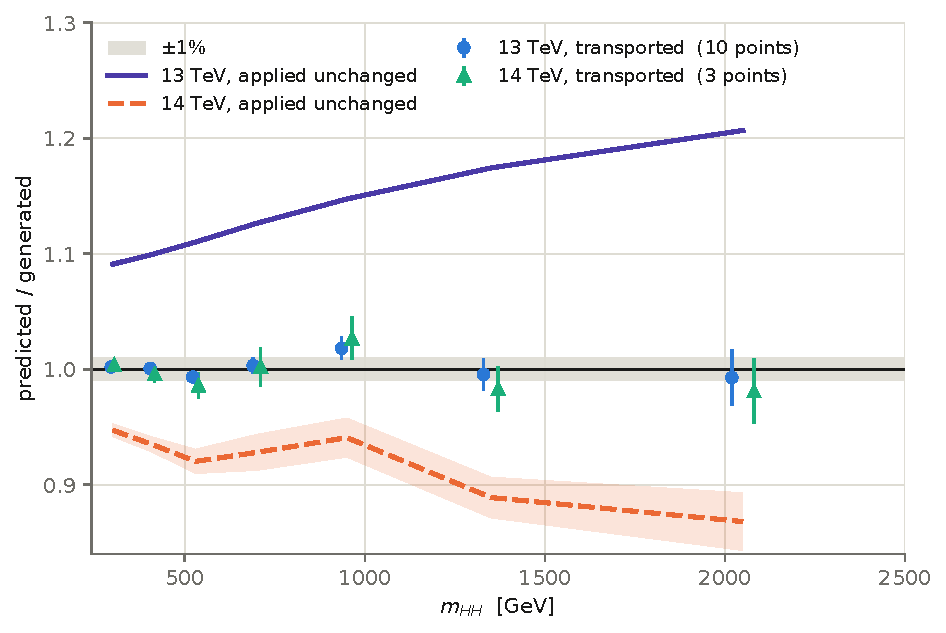
\includegraphics[width=0.49\linewidth]{plots/energy_transport_13TeV.pdf}
\hfill
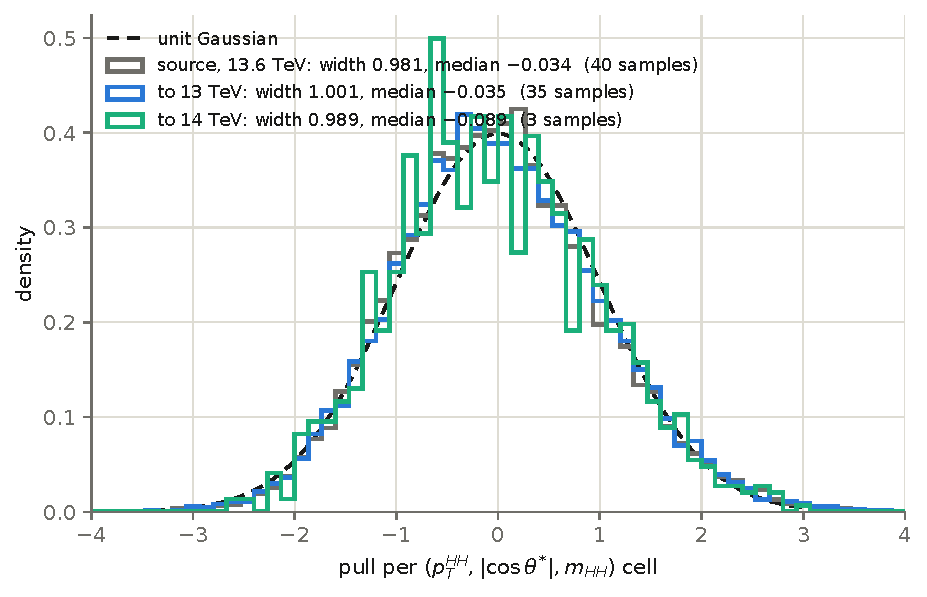
\includegraphics[width=0.49\linewidth]{plots/energy_coeff_pulls_3d.pdf}
\caption{Left: ratio of predicted to generated \mHH spectrum at $13$ and $14$~TeV, with
the $13.6$~TeV parameterization applied unchanged (lines) and transported with
Eq.~\eqref{eq:energy_kernel} (points, overall constant removed); the band marks
$\pm 1\%$. Right: pull of the transported $A$-coefficients per
$(\pt^{HH}, |\cos\theta^*|, \mHH)$ cell, on the basis points, against a unit Gaussian
(dashed). Both are described in the text.}
\label{fig:energy_transport}
\label{fig:energy_coeff_pulls}
\end{figure}

\textcolor{red}{Matheus: the complete forty-point basis is being generated at every
energy --- five points are missing at $13$~TeV and thirty-seven at $14$~TeV, the former a
subset of the latter, so it is one request. With those in hand the right panel closes on
the full basis at all three energies, with no caveat about which subset was available,
and the $14$~TeV pull width goes from an uncertainty of $\pm 1.3$, which says nothing, to
about $\pm 0.03$.}

\paragraph{Two further checks.}
The kernel of Eq.~\eqref{eq:energy_kernel} is exactly invertible, so running the machinery
in the opposite direction --- transporting the $13$~TeV samples up to $13.6$~TeV --- must
return the inverse constant. It does, $1.0098$ against $1/0.9902 = 1.0099$, which is a
check on the implementation and not on the physics.

The second check is the configuration an analysis actually deploys. Only the forty basis
templates are transported; every other coupling point is then built from them by the
matrix method, whose weights are the same at every energy. Closing the morphed prediction
against the reweighting samples of Sec.~\ref{sec:grids} leaves the agreement unchanged in
the bulk, and in the tail the comparison becomes limited by the statistics of the basis
samples themselves, amplified by the morphing weights: the matrix method's own statistical
uncertainty on the morphed prediction is $8\%$ per bin below $1$~TeV and $38\%$ above it,
and every per-bin deviation lies within $0.6$ of that uncertainty, with a mean pull of
zero. The transport introduces no bias that the available statistics can detect; what
limits the tail is the size of the basis samples, not the transport.

\paragraph{The covariance.}
The coefficients are delivered with their covariance, and it has to be transported
too. Because the kernel multiplies all forty coefficients of a cell by the same
number, the covariance of that cell transforms quadratically rather than linearly:
%
\begin{equation}
C_{kl}(\sqrt{s}',j) = K_j^2 \left[ C_{kl}(\sqrt{s},j)
                      + r_j^2\, A_k^j A_l^j \right] ,
\label{eq:energy_cov}
\end{equation}
%
where $r_j$ is the relative statistical uncertainty of $K_j$. The factor $K^2$ is the
part that is easy to get wrong: reusing the $13.6$~TeV covariance unchanged would
leave the uncertainties $30\%$ too large at $13$~TeV and $8\%$ too small at $14$, in
opposite directions.

The second term is the uncertainty of the kernel itself. It is rank one and fully
correlated across the forty coefficients of a cell, so it does not average down
within a cell, and it is not negligible: $r$ has a median of $1.8\%$ per cell, while
a quarter of the $57600$ coefficient entries carry a relative uncertainty smaller than
that. Where the one-dimensional region or a noisy cell makes the transport fall back on
the \mHH-projected kernel, $r$ is the projected kernel's own uncertainty, $0.3\%$,
since that is measured on all $36$ $\pt$--$|\cos\theta^*|$ cells together.

Two uncertainties are deliberately left outside Eq.~\eqref{eq:energy_cov} because a
per-cell matrix cannot express them. The parton-density uncertainty on $K$ is
correlated between bins, and the overall normalization of the transport is a single
number correlated across every bin and coefficient; both are carried as nuisance
parameters alongside.

\subsection{Beyond the LHC}
\label{sec:energy_beyond}

\textcolor{red}{PLACEHOLDER. The transport is not used for the $100$~TeV results.
Reweighting redistributes the events that exist; it cannot create an event at a partonic $\hat{s}$ the source sample
never produced. The $13.6$~TeV samples place $7.5\times 10^{-5}$ of their rate above
$3$~TeV and the highest bin holding more than a thousand effective events is
$3.75$~TeV, so a transported $100$~TeV prediction would be blind in exactly the region
that motivates such a collider. The kernel is also no longer gentle --- median $30$,
spanning $5$ to $270$, with weights reaching $3800$ --- and it costs between a half and
two thirds of the effective sample size. The $100$~TeV coefficients are therefore
extracted from $100$~TeV simulation in the usual way, and the basis is re-optimized
there rather than inherited.}


\clearpage
\section{Uncertainty prescription}
\label{sec:uncertainties}

The matrix method predicts $N(\mathbf{c})=\sum_i w_i(\mathbf{c})\,N_i$, so the
statistical error of the basis templates propagates with the same weights,
\begin{equation}
\sigma^2_\mathrm{interp}(\mathbf{c}) \;=\; \sum_i w_i(\mathbf{c})^2\,\sigma_i^2 \;,
\label{eq:sigmainterp}
\end{equation}
evaluated independently in every bin. The equation separates into two factors with
different owners: the weights are a property of the basis, published once and the same
in every bin, and the $\sigma_i$ are a property of whichever templates the weights are
applied to. The band is therefore wide where the templates are thin and narrow where
they are populated, which a prescription built from the total rate cannot reproduce.

The size of the band along a coupling scan depends on the templates it is propagated
through, and so on the selection; Sec.~\ref{sec:validation_realistic_band} measures it
for two real selections. For the inclusive cross section it is largest where the yield
is smallest: $0.2\mbox{--}5.8\%$ along $c_\PH$, peaking at the cancellation near
$c_\PH\simeq-3$ where the cross section falls to $13$~fb, and $0.3\mbox{--}0.7\%$ along
$c_{\PH\mathrm{kin}}$. All nine scans pass through $0.50\%$ at the SM and stay below
$1.5\%$ except $c_\PH$ and $c_{\PH G}$, which reach $5.8\%$ and $5.1\%$; the rest are in
App.~\ref{sec:appendix_performance}. The relative band grows as the rate falls, the
absolute error being set by the templates and not by the point predicted. The two scans
differ by almost an order of magnitude in their worst case despite minima of comparable
depth, which is a property of the basis: $c_{\PH\mathrm{kin}}$ is covered by more basis
points at the relevant values, so the interpolation reaches it with smaller weights.

The band is calibrated against the scatter observed along a scan, which is the direction
a fit moves in. For every generated sample on a line through the grid, the median
absolute residual over bins is compared with the median that pure statistics would give,
$0.674\sqrt{\sigma^2_\mathrm{interp}+\sigma^2_\mathrm{stat}}$; a correctly sized band
puts the ratio at one. Averaged over the $c_\PH$--$c_{\PQt\PH}$ plane the ratio is
$0.74$, and the fraction of bins whose pull is within one standard deviation is $0.72$
against the $0.683$ of a standard normal; along the individual scans of that plane it
stays between $0.6$ and $0.9$ with no trend in one region or another. Four further
planes give ratios of $0.65$ to $0.88$ and coverages of $0.67$ to $0.76$, collected in
Tab.~\ref{tab:unc_calibration}. The band therefore covers the observed scatter, by some
$25\%$ conservatively.

Two limitations are inherited from the inputs. The $\sigma_i$ are estimated from the
event count and the negative-weight fraction of each sample, because the sample set does
not record per-bin sums of squared weights; the per-bin estimate is supported by the
pull being close to normal, while the same quantity built from the total rate is about
six times wider than the observed residual and must not be used. The second is specific
to the scans of this section: the basis templates are themselves samples of the grid the
reweighting coefficients were fitted to, so adding the interpolation uncertainty to the
uncertainty of those coefficients double counts. It amounts to forty samples of some
four thousand, with a coefficient term well below the interpolation one, and it does not
arise in the case an analysis faces, where the templates are built from its own events
and the coefficients come from the grid.

What does arise there is a correlation between templates built from the same events.
Eq.~\eqref{eq:sigmainterp} treats the $\sigma_i$ as independent, which is exact where
the basis templates are separately generated samples --- the case for every number
quoted in this section and for the calibration above --- and not where they are produced
by reweighting one set of events, as those of
Sec.~\ref{sec:validation_realistic_band} are. The exact variance is a quadratic form in
the same weights,
\begin{equation}
  \sigma^2_\mathrm{MM}(\mathbf{c}) = w(\mathbf{c})^{T} S\, w(\mathbf{c}),
  \qquad
  S_{ik} = \sum_s \alpha_s(i)\,\alpha_s(k) \sum_{e \in s} \omega_i(e)\,\omega_k(e),
  \label{eq:sigmaMMcov}
\end{equation}
evaluated in each bin, with $\omega_i(e)$ the weight that takes event $e$ to basis point
$i$ and $\alpha_s(i)$ the inverse-variance weight with which input sample $s$ enters
template $i$ in that bin. Its diagonal is the error each template carries on its own, so
Eq.~\eqref{eq:sigmainterp} is the case $S$ diagonal.

The two forms differ by factors rather than by percents. Measured on the \HHbbbb templates with
$S$ built per \mHH bin, they agree at a basis point, where the weight vector is a unit
vector, and depart from one another elsewhere: integrated over \mHH the independent form
is between $0.7$ and $9$ times the exact one over the points tested, and bin by bin
between $0.6$ and about $30$, mostly above it, the departure growing with
$\sum_i|w_i|$. The templates are reweightings of the same events, so their fluctuations
cancel in the morphed sum where the independent form adds them in quadrature. An
analysis whose templates come from a common set of events should therefore use
Eq.~\eqref{eq:sigmaMMcov}, which costs one pass over its own events with every basis
point's weight, or propagate the uncertainty through the reweighting evaluated directly
at the point in question, which carries the correlation automatically.

Fig.~\ref{fig:unc_band_by_bin} resolves the band into the \mHH bins it is computed from,
at four points of the $c_\PH$ scan. In every bin the weights are the same; what differs
is how many events the basis templates have there. The band is below $1\%$ near
threshold, where the templates are well populated, and reaches tens to hundreds of
percent above $1.5$~TeV, where they hold few events. The curve at $c_\PH=-3$ is large at
low mass as well: there the prediction is a difference of comparable contributions, so a
small absolute error on the templates is a large relative error on what survives.

\begin{figure}[htbp]
    \centering
    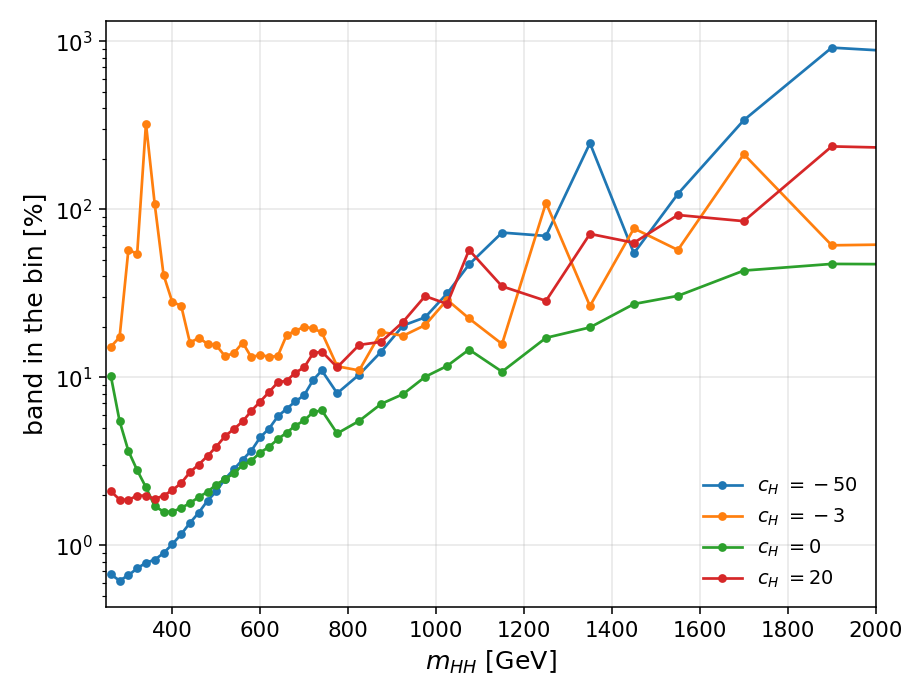
\includegraphics[width=0.49\textwidth]
        {figures/basis_optimization/unc_band_by_bin.png}%
    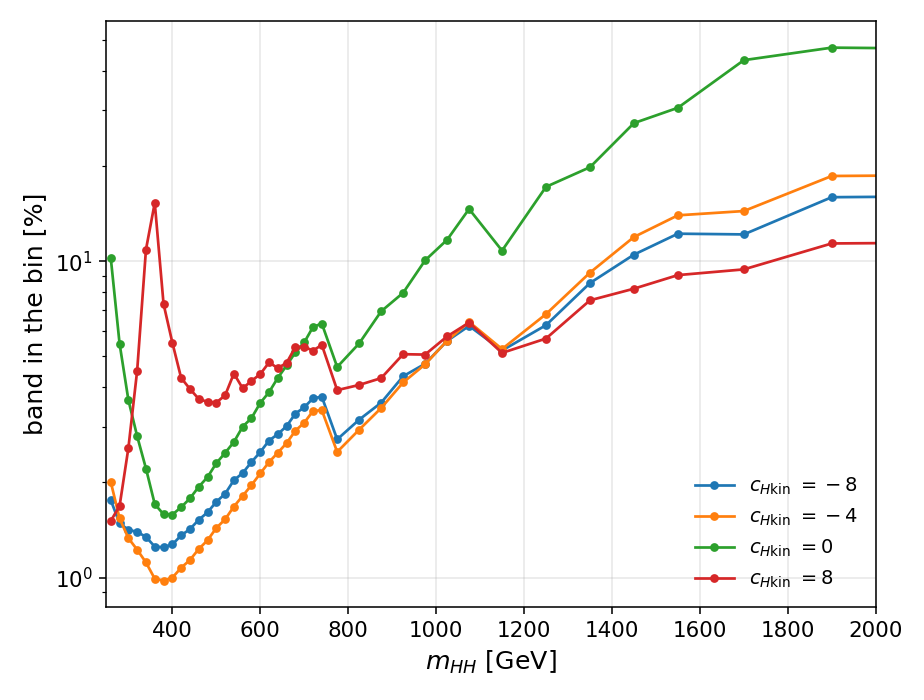
\includegraphics[width=0.49\textwidth]
        {figures/basis_optimization/unc_band_by_bin_cHkin.png}
    \caption{Interpolation uncertainty of Eq.~\eqref{eq:sigmainterp} in each
    \mHH bin, as a fraction of the predicted content of that bin, at four
    values of $c_\PH$ (left) and of $c_{\PH\mathrm{kin}}$ (right), the other
    eight coefficients at zero in each case.}
    \label{fig:unc_band_by_bin}
\end{figure}

Integrated over \mHH the same band is a few percent, which is why the prescription has
to be differential. The bins with the largest relative uncertainty carry almost none of
the yield, so summing over bins lets the well-populated low-mass bins dominate and
the tail contribute little. A number quoted from the total alone would be those few
percent and would not record that part of the spectrum is predicted only to within a
factor, which is what an analysis fitting the tail needs.

That separation is measured in Sec.~\ref{sec:validation_realistic_band}, where the
weights published here are applied to the templates of two different $\HH\to\bbbar\bbbar$ selections and
give two bands differing by a factor of five to ten, with nothing about the effective
field theory re-derived in between. The prescription transfers; the numbers quoted in
this section do not.

In a fit the band need not be evaluated at all. Since
$N_j(\mathbf{c})=\sum_i w_i(\mathbf{c})N_{ij}$, giving each basis template its own
statistical uncertainty and letting the fit recompute the sum with the varied templates
reproduces Eq.~\eqref{eq:sigmainterp}, carries its dependence on $\mathbf{c}$, and keeps
the cancellations between weights of opposite sign. Where the forty templates are
themselves the inputs the model morphs, an automatic treatment of the template
statistics already does this. Precomputing the band at one coupling point and quoting it
as a fixed shape uncertainty is adequate only near the SM: over the generated ranges the
band varies by an order of magnitude.

The uncertainty of the reweighting coefficients the templates were made with is a
separate term and stays one nuisance. It is a single source, correlated across templates
and bins, so a coherent shift of it partly cancels in the weighted sum where the
independent statistical errors add in quadrature, and treating it as one nuisance per
template would overstate it. It is the larger of the two in the resolved selection for
every coefficient of Fig.~\ref{fig:acc_4b}, so a prediction carrying only the template
statistics understates its total modelling uncertainty by a factor of a few. The two are
combined as $\sigma_\mathrm{mod}^2=\sigma_\mathrm{MM}^2+\sigma_\mathrm{ELR}^2$ and are
given separately per selection in Tab.~\ref{tab:unc_components}.

A card built this way carries three terms that do not overlap. The Monte Carlo
statistical uncertainty of the background enters through the Barlow--Beeston-lite
treatment of Combine, which leaves the signal processes out; that of the morphed signal
enters through one nuisance parameter per channel of size
$\sigma_\mathrm{MM}(\mathbf{c})/N(\mathbf{c})$, computed from the covariance of the basis
templates and following the coefficients as they move; and the reweighting coefficients enter as the single
correlated nuisance parameter described above.

Beyond the interpolation, the \ggHH prediction carries its own theory uncertainty, and
the nine-coefficient model inherits it from the $\kappa$ models unchanged: the QCD scale
and top-mass envelope of the non-resonant \ggHH cross section, applied as a single
nuisance scaling every \ggHH sample alike. The envelope is tabulated against
$\kappa_\lambda$, so the model evaluates it at the $\kappa_\lambda$ obtained from the
Wilson coefficients by the naive translation of Eq.~\eqref{eq:naivetranslation}, which at
$\Lambda=1$~TeV reads $\kappa_\lambda = 1 - 0.469\,c_\PH + 0.182\,c_{\PH\mathrm{kin}}$.
Being a common factor of all \ggHH samples it does not interact with the morphing: it
multiplies the prediction after the templates are combined, and is unaffected by the
restriction of Sec.~\ref{sec:slice_models}, since the templates left out there have a
vanishing morphing weight.

Two properties of that prescription follow. The envelope is not re-expressed as
a function of the Wilson coefficients: it is the $\kappa_\lambda$ envelope evaluated at
the translated point, so it remains the same object the $\kappa$ models use and follows
any update to it. Writing it out in $c_\PH$ instead would fix $\Lambda$, since the
translation carries $v^2/\Lambda^2$, and an analysis at a different $\Lambda$ would
silently get the wrong uncertainty. The envelope also covers only the trilinear
direction: it was built by varying $\kappa_\lambda$, so the part of
$c_{\PH\mathrm{kin}}$ that rescales the top Yukawa, and the scale dependence introduced
by the operators with no $\kappa_\lambda$ image, are not included in it.


\clearpage
\section{Modeling a truncated prediction}
\label{sec:trunc_modelling}

Both the usual truncation schemes, linear and quadratic, are covered by the tools discussed so far ($A$-coefficients/ELR and MM). The former keeps only the SM interference with dimension-six operators at the cross section level, therefore neglecting all terms of order $1/\Lambda^4$. The later defines the expansion at the amplitude level, $\mathcal{M}=\mathcal{M}_{\text{SM}}+\mathcal{M}_{\text{dim6}}$, therefore carrying terms of order $|\mathcal{M}_{\text{dim6}}|^2\sim1/\Lambda^4$ at the cross section level---but missing terms originating from SM times double dimension-6 insertions, $\sigma_{\text{SM}\times\text{dim6}^2}\sim\mathcal{O}(1/\Lambda^4)$, an additional interference that would require contributions from dimension-8 operators. The caveat of adding subleading operators is that those have an extra loop suppression and therefore contribute only linearly in the cross section. In this regard power counting-wise, the quadratic components of the subleading operators are closer to the contributions coming from the first dimension-8 contributions, similarly to the double insertion of leading operators. 

As reference, we generate some of the benchmarks discussed in Ref.~\cite{Bär:2965348} with the PDF set \texttt{PDF4LHC\_21} in both truncations, and compare the results obtained from the $A$-coefficients and by the MM approach. The resulting distributions are shown in Figure \ref{fig:linearquad}. The linear truncation is achieved by switching off the $A$-coefficients related to the quadratic components shown in Table \ref{fig:linearquad}. For the MM, the basis samples were generated with the linear truncation and solved the coefficients bin by bin, restricting the sum to the ten linear monomials at evaluation. The total
cross sections agree with the simulation to $1.3$--$2.2\%$ at BM1 and BM2 and to $3.5\%$
at BM5, in the quadratic and in the linear truncation. At BM4 the linearly truncated
prediction is negative, $-0.045$~pb against $-0.041$~pb in the generated sample, whose
event weights are negative in $98\%$ of events, so the method follows the truncation into
that region as well. 


%Sec.~\ref{sec:truncation} states over what range of the Wilson coefficients a chosen
%dimension-6 truncation is one an analysis would want. This section asks the separate
%question of whether the tools of this report reproduce that truncation once it is chosen:
%whether a prediction truncated at the interference term, or at the leading quadratic
%terms, is described as well as the complete one, by the reweighting evaluated directly and
%by the matrix method on the optimized basis alike. Both are needed, because an analysis
%quoting a linear result has to produce it with the same machinery it uses for everything
%else.

%The truncation is the choice of which powers of $1/\Lambda^2$ are kept in the polynomial.
%The results of this report use the quadratic truncation for the leading operators and the
%linear one for the subleading operators, the option \texttt{b} of \texttt{POWHEG-BOX-V2}
%combined with $\textsc{includesubleading}==1$ of Sec.~\ref{sec:parameterization}. That
%choice fixes both the normalization and the \mHH and \pt shapes away from the SM point,
%by an amount that grows with the Wilson coefficients and, for the operators that generate
%energy-growing amplitudes, with the momentum transfer.

%The study needs no additional coefficient fit. Eq.~\eqref{eq:smeftpara_reorg} \emph{is} the
%truncated cross section, organized bracket by bracket in
%Table~\ref{tab:smeft_matrix_blocks}, so a change of truncation amounts to including or
%dropping one group of $A$-coefficients. All 40 coefficients have already been extracted,
%per bin and at each energy (Sec.~\ref{sec:extraction}), and every truncation is a different
%subset of the same 40 numbers. The only simulated input entering this section is the set of
%benchmark samples described below.

%\textcolor{red}{DEFERRED to Sec.~\ref{sec:energy_beyond}: the inclusive ratio
%$\sigma_{\text{trunc}}/\sigma_{\text{nom}}$ along one-dimensional rays, and the same
%ratio differentially, are better shown at the two energies together than at $13.6$~TeV
%alone. The $13.6$~TeV halves can be produced today from the $A$-coefficients fitted to
%the generated samples; the $100$~TeV halves wait on that extraction.}

%Three predictions are compared, all read off the same coefficient set. The \emph{linear}
%one keeps the SM term $A^j_0$ with the linear brackets only, the leading terms
%$A^j_1$--$A^j_4$ and the subleading terms $A^j_{15}$--$A^j_{19}$; it is the strictly
%dimension-6 interference prediction. The \emph{leading-quadratic} one adds the leading-only
%quadratic block $A^j_5$--$A^j_{14}$. The \emph{nominal} one adds the
%leading$\,\times\,$subleading block $A^j_{20}$--$A^j_{39}$ and is the truncation used
%throughout this report. The only dimension-6 squared terms absent from all three are the
%purely subleading squares, dropped in the generation (Sec.~\ref{sec:parameterization});
%they are not accessible from these coefficients.

%Ref.~\cite{Bär:2965348} defines a set of \HH benchmark points in the same operator space
%and provides, for each, a prediction generated separately in the linear and in the
%quadratic truncation. They are an external test rather than two evaluations of one fit: each truncated
%prediction is compared with the simulation produced with that truncation, so an error in
%the bracket bookkeeping would appear in one truncation while the other still closed. Four of them are used here, defined
%y $c_\PH=3$; $c_\PH=-2$, $c_{\PH\mathrm{kin}}=-2$, $c_{\PQt\PH}=4$; $c_\PH=-6$; and
%$c_\PH=-3$, $c_{\PH\mathrm{kin}}=-2$, $c_{\PQt\PH}=0.5$, all other coefficients at zero.

%The comparison is shown in Fig.~\ref{fig:linearquad}. In each panel the polynomial
%reproduces the generated spectrum in the linear and in the quadratic truncation alike, so
%the $A$-coefficients describe not only the nominal prediction but each of its truncations
%separately. The same holds for the other route. Taking the forty-point basis with its templates from
%the generated samples, solving for the coefficients bin by bin and restricting the sum to
%the ten linear monomials at evaluation reproduces the same generated spectra: the total
%cross sections agree with the simulation to $1.3$--$2.2\%$ at BM1 and BM2 and to $3.5\%$
%at BM5, in the nominal and in the linear truncation alike. At BM4 the linearly truncated
%prediction is negative, $-0.045$~pb against $-0.041$~pb in the generated sample, whose
%event weights are negative in $98\%$ of events, so the method follows the truncation into
%that region as well. Both tools therefore model each truncation, and both close against
%simulation when truncated as they do when complete.

%These benchmark samples were generated with \texttt{PDF4LHC21\_40}, a newer set
%than the \texttt{PDF4LHC15\_nlo\_30\_pdfas} used for the samples the coefficients were
%fitted from (Sec.~\ref{sec:eventsimulation}), and the panels close over the whole \mHH
%range notwithstanding. The reweighting is a ratio of cross sections evaluated at
%the same kinematics, so a change of parton densities largely cancels in it, and the
%closure across two different sets measures what does not cancel. The separation between the two sets of
%curves within a panel is the truncation effect itself, at coupling values of order a few.
%The benchmark at $c_\PH=-6$ shows the other practical consequence of truncating at the
%interference term: a strictly linear cross section is of first degree in the Wilson
%coefficients and carries no positivity guarantee once the interference overwhelms the
%SM term, and the vertical scale of that panel accordingly reaches negative
%values.

\begin{figure}[t]
  \centering
  \begin{minipage}[b]{0.495\linewidth}
    \centering
    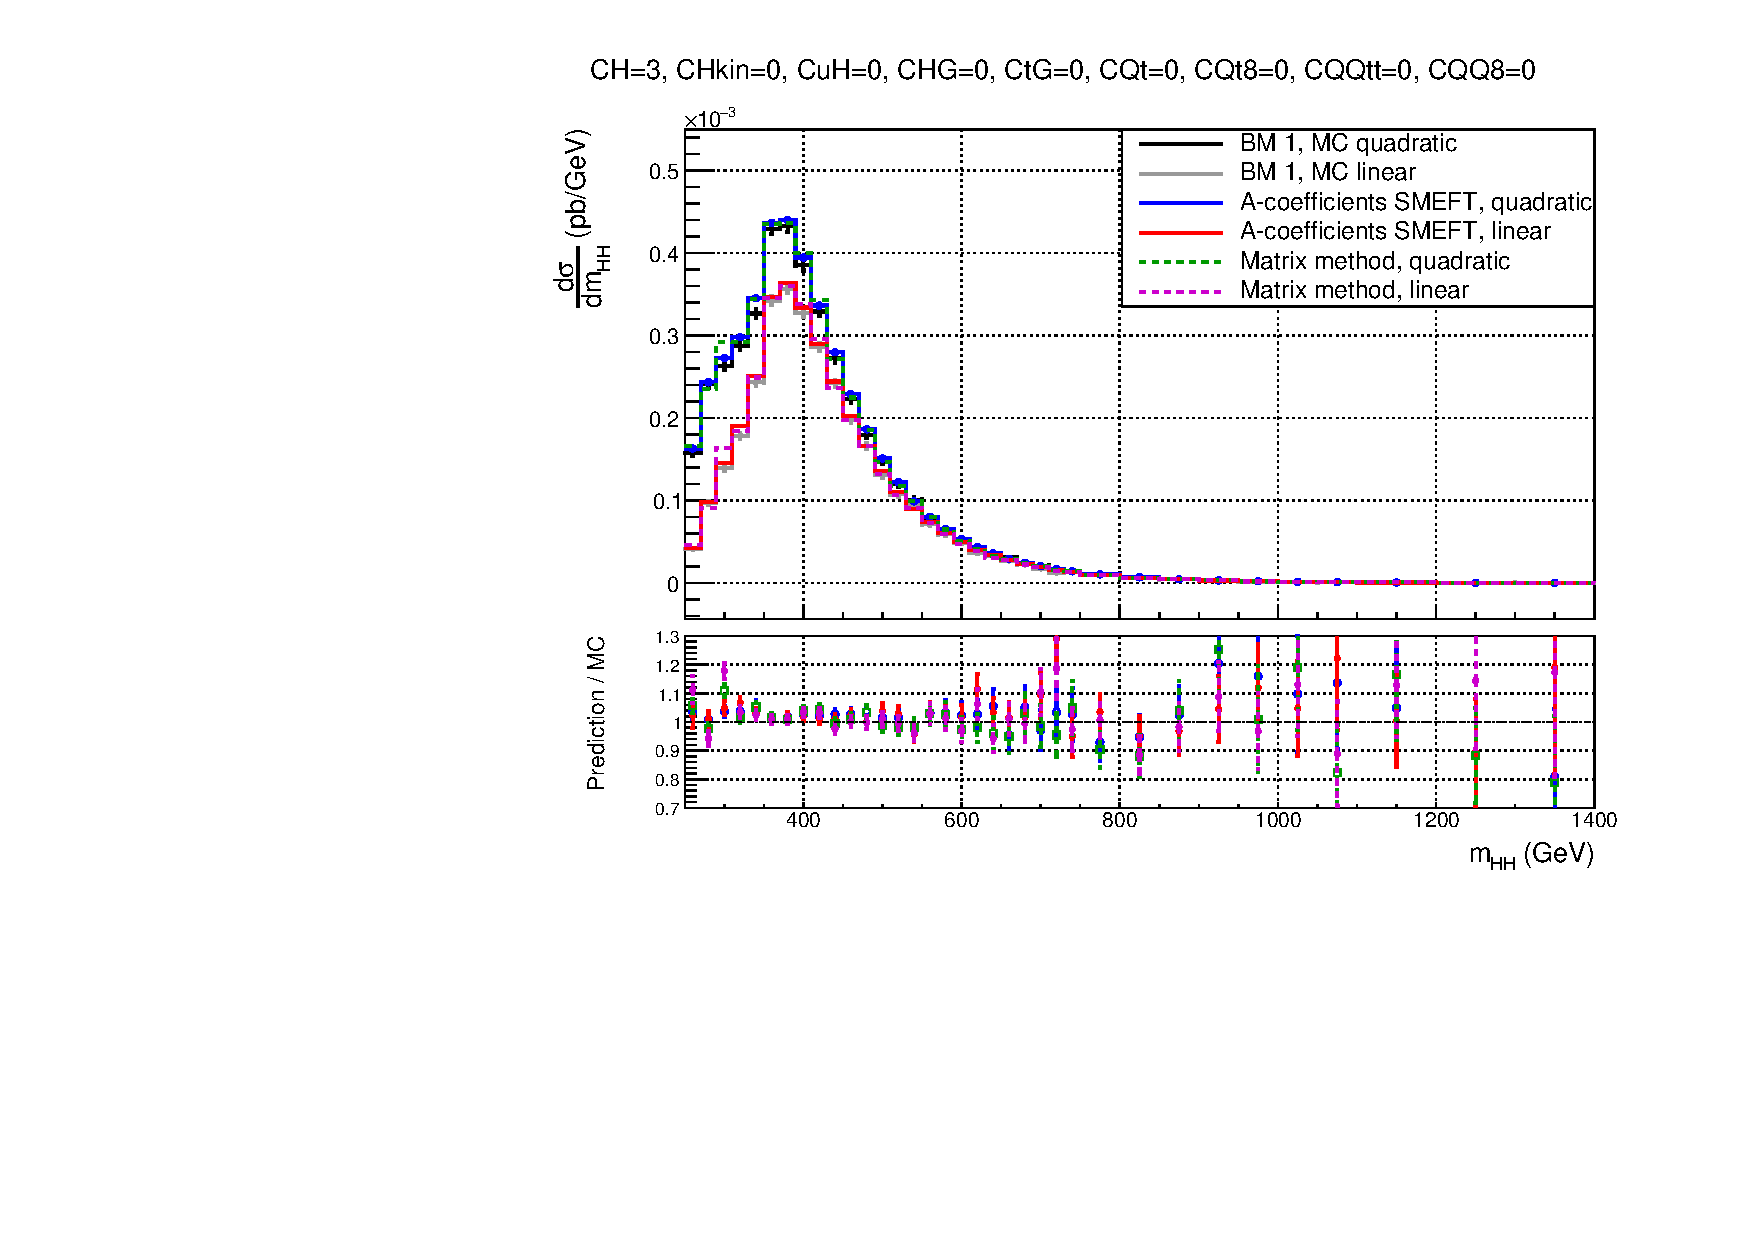
\includegraphics[width=\linewidth]{plots/poly_3d_9D_trunc_linvsquad_MM_(5)_CH_3.0_CHbox_0.0_CuH_0.0_CHG_0.0_CtG_0.0_CQt_0.0_CQt8_0.0_CQQtt_0.0_CQQ8_0.0.pdf}
  \end{minipage}
  \hfill
  \begin{minipage}[b]{0.495\linewidth}
    \centering
    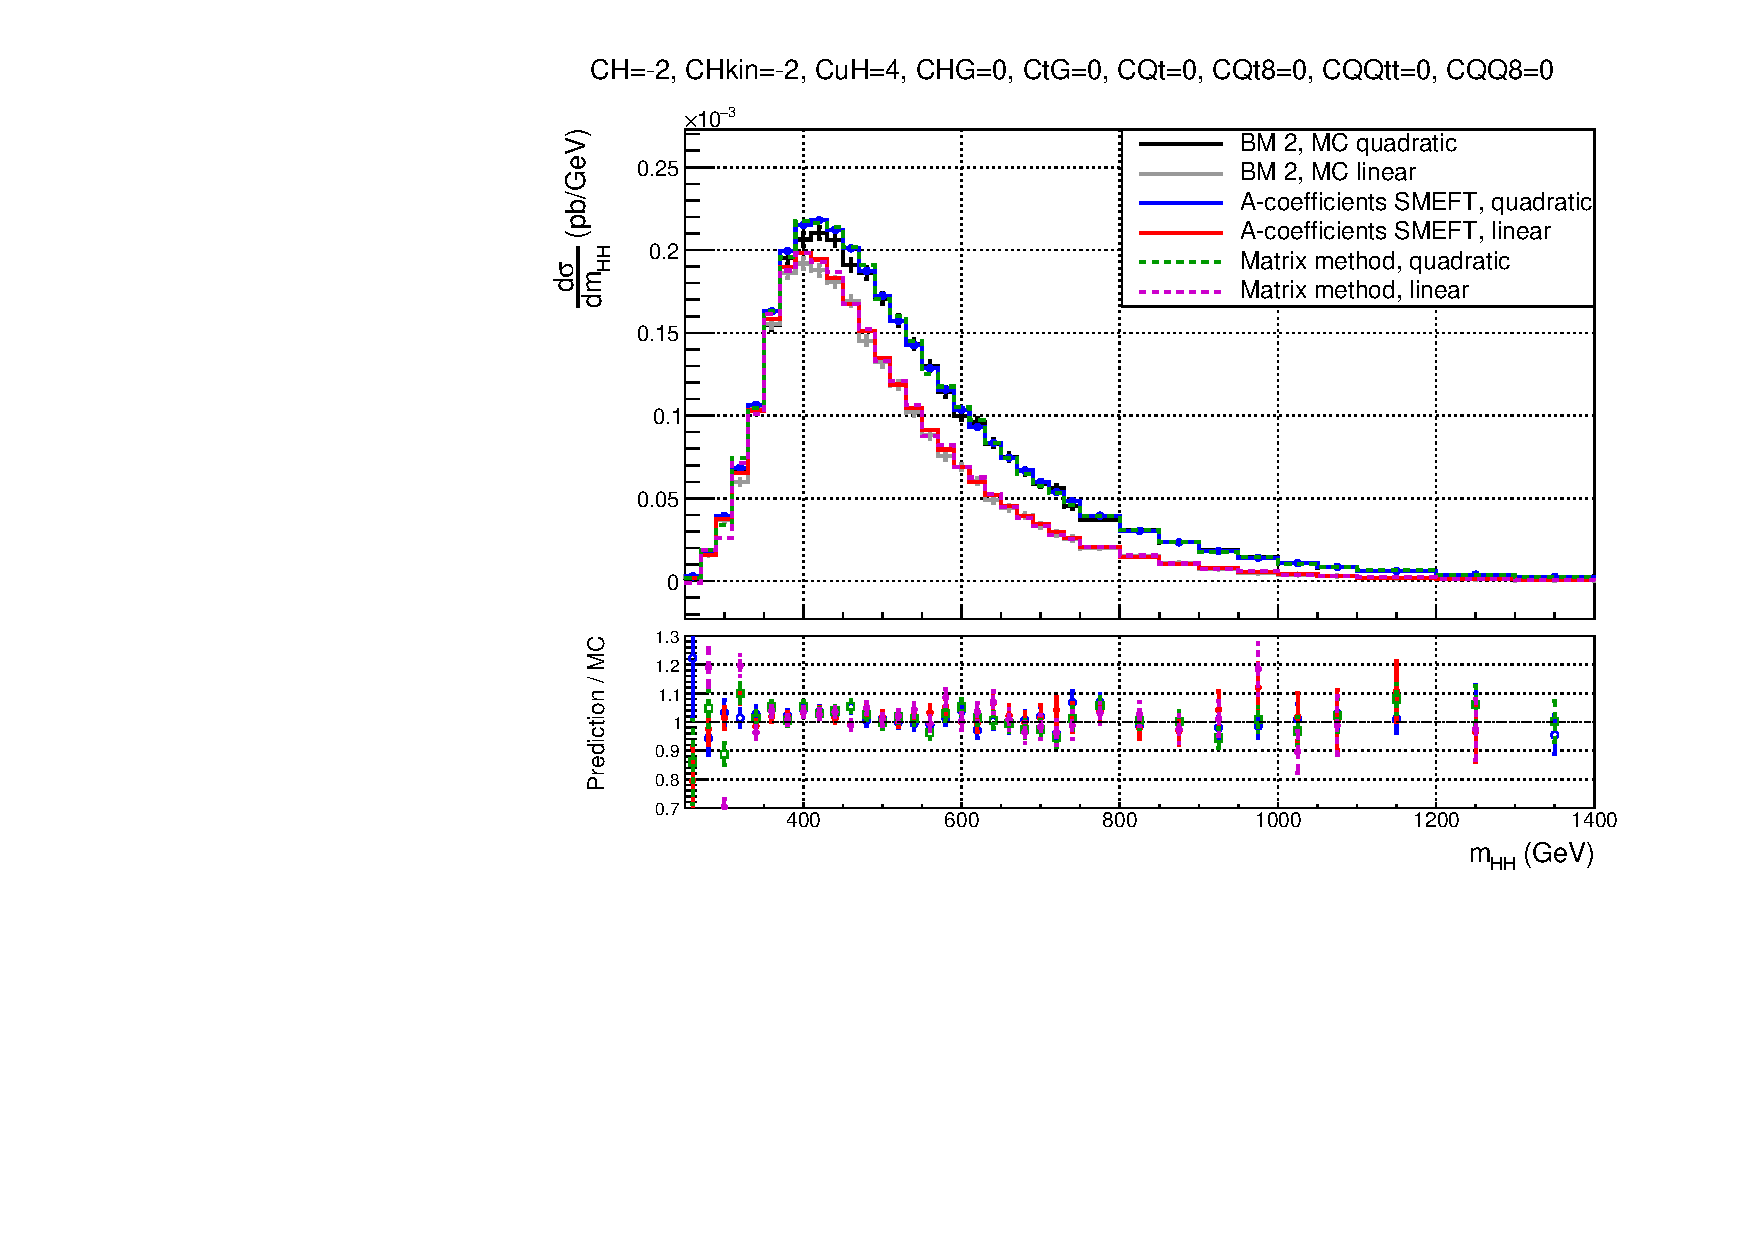
\includegraphics[width=\linewidth]{plots/poly_3d_9D_trunc_linvsquad_MM_(4)_CH_-2.0_CHbox_-2.0_CuH_4.0_CHG_0.0_CtG_0.0_CQt_0.0_CQt8_0.0_CQQtt_0.0_CQQ8_0.0.pdf}
  \end{minipage}
  \vspace{0.5em}
  \begin{minipage}[b]{0.495\linewidth}
    \centering
    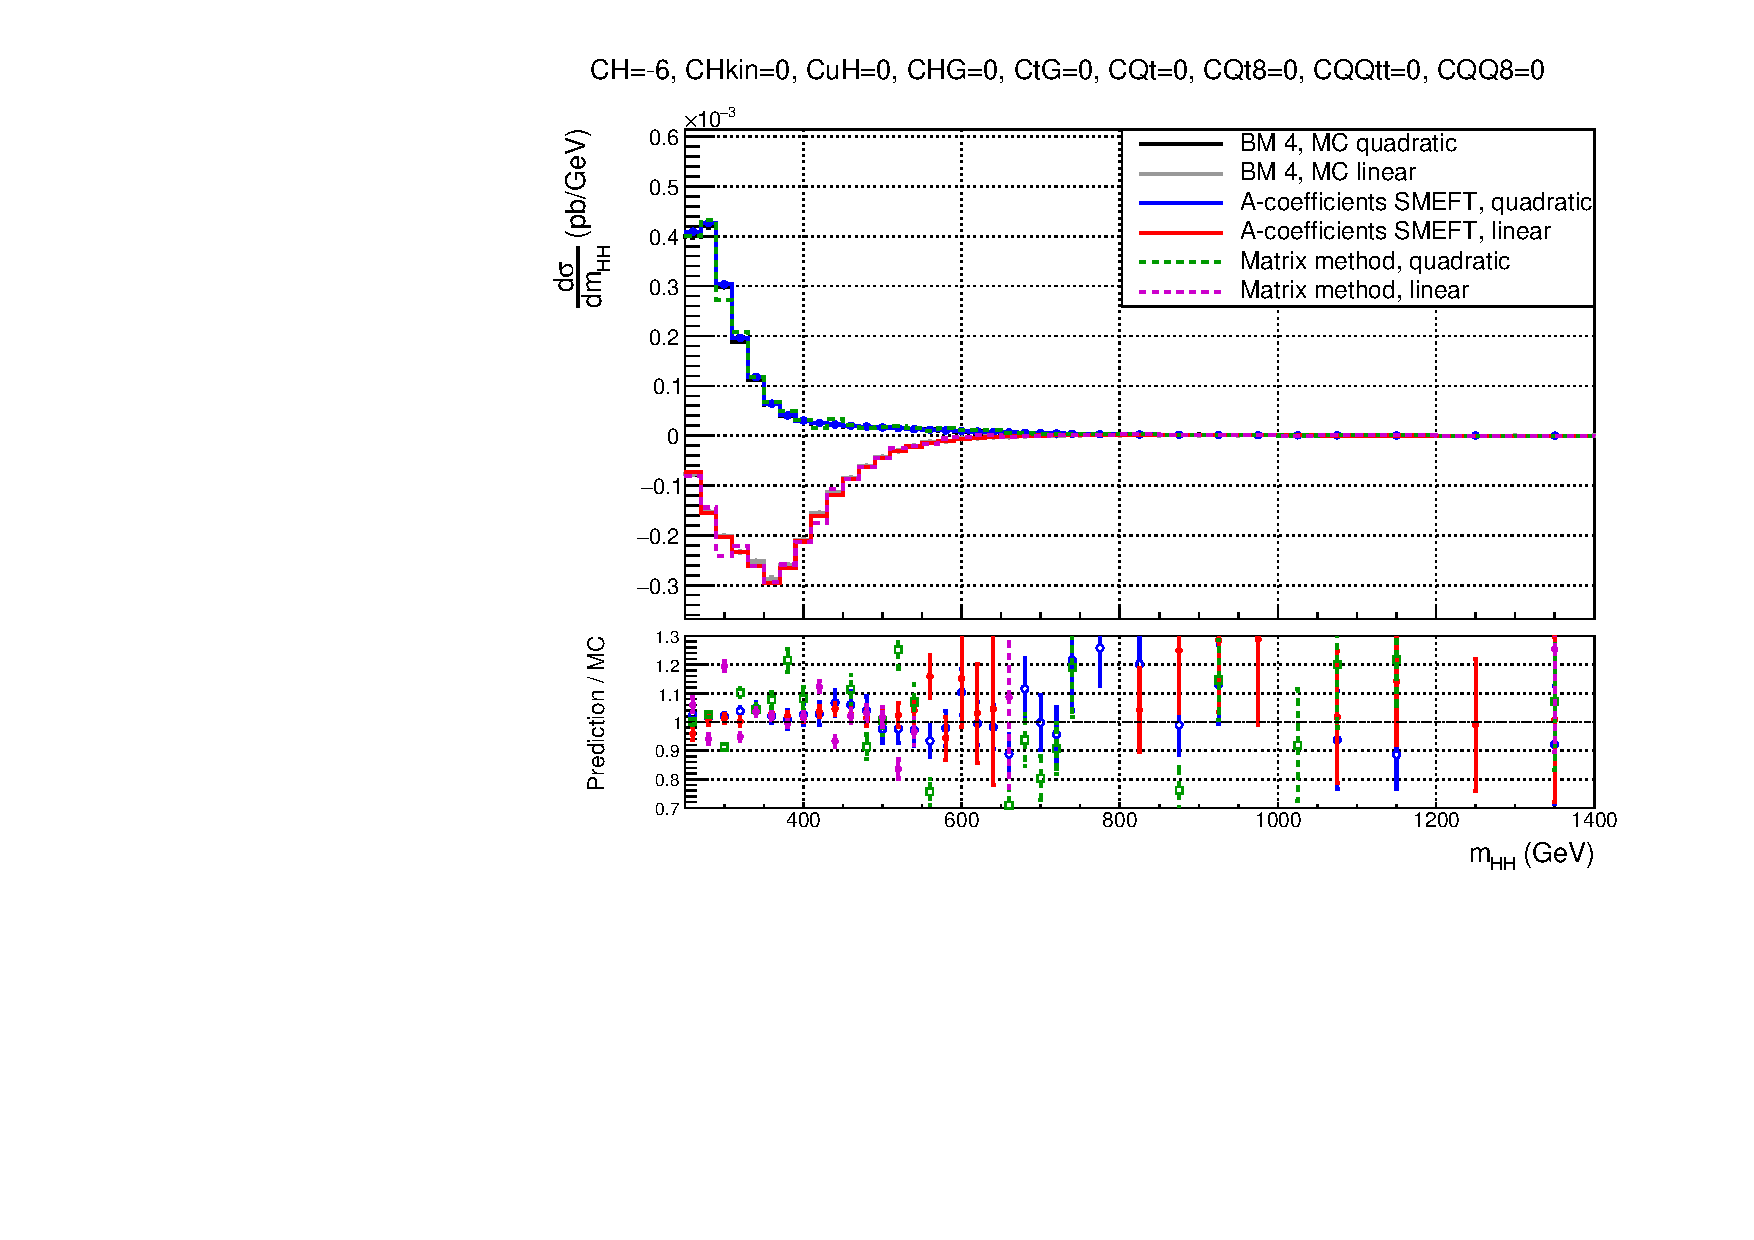
\includegraphics[width=\linewidth]{plots/poly_3d_9D_trunc_linvsquad_MM_(1)_CH_-6.0_CHbox_0.0_CuH_0.0_CHG_0.0_CtG_0.0_CQt_0.0_CQt8_0.0_CQQtt_0.0_CQQ8_0.0.pdf}
  \end{minipage}
  \hfill
  \begin{minipage}[b]{0.495\linewidth}
    \centering
    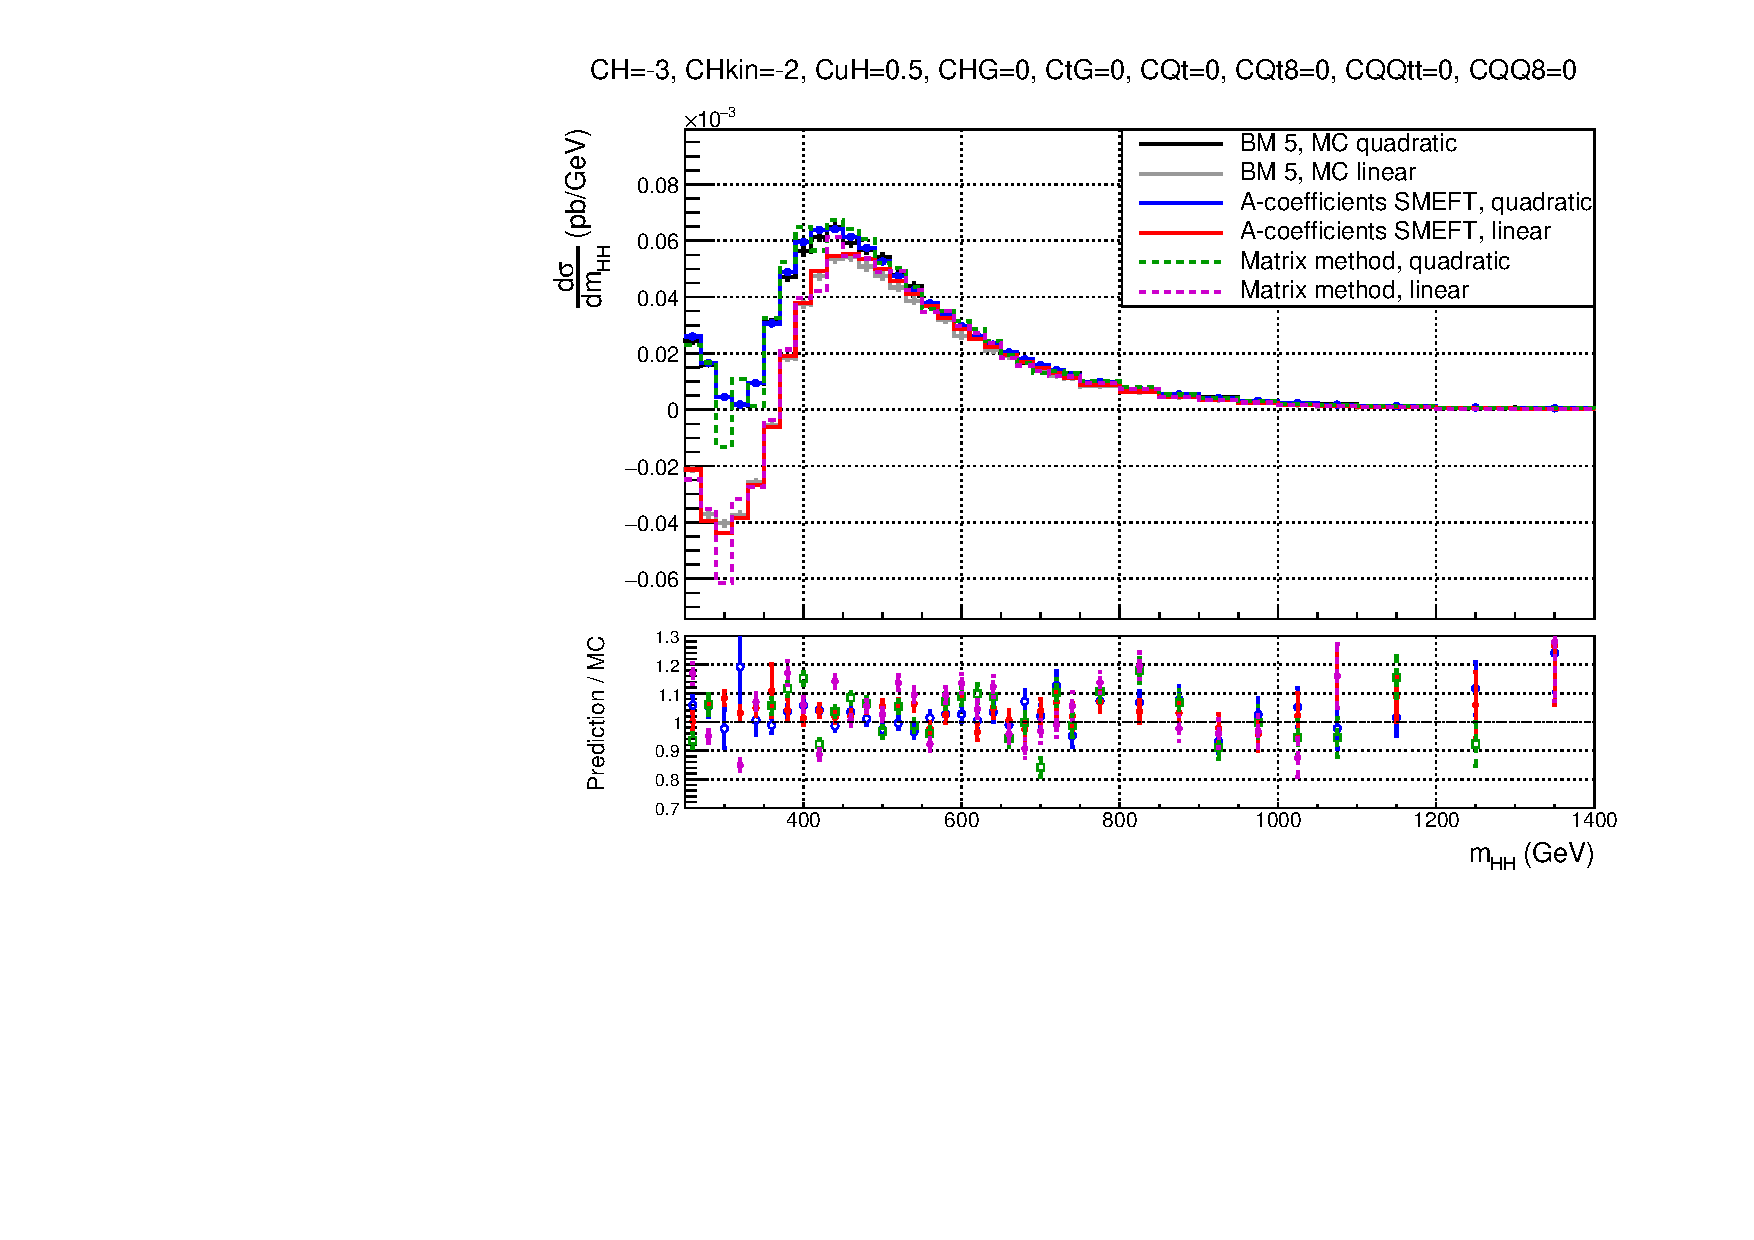
\includegraphics[width=\linewidth]{plots/poly_3d_9D_trunc_linvsquad_MM_(2)_CH_-3.0_CHbox_-2.0_CuH_0.5_CHG_0.0_CtG_0.0_CQt_0.0_CQt8_0.0_CQQtt_0.0_CQQ8_0.0.pdf}
  \end{minipage}
  \caption{Differential cross section in \mHH for four of the benchmark points defined in Ref.~\cite{Bär:2965348}: BM~1, $c_\PH=3$ (top left); BM~2, $c_\PH=-2$, $c_{\PH\mathrm{kin}}=-2$, $c_{\PQt\PH}=4$ (top right); BM~4, $c_\PH=-6$ (bottom left); and BM~5, $c_\PH=-3$, $c_{\PH\mathrm{kin}}=-2$, $c_{\PQt\PH}=0.5$ (bottom right). All other Wilson coefficients are zero. Each panel shows the samples generated at that point in the linear and in the quadratic truncation, together with the corresponding predictions of the 3D $A$-coefficient parameterization projected onto \mHH and the results obtained from MM. The lower pad gives the ratio of the parameterization to the simulation.}
%\textcolor{red}{The matrix-method curves, nominal and linearly truncated, are still to
%be overlaid on these panels; the request and the location of the histograms are in the
%text below. This sentence comes out once the curves are in.}}
  \label{fig:linearquad}
\end{figure}

% --- three figures still to be produced; the request is in the text above ---
% \newcommand{\truncplaceholder}[1]{%
%   \fbox{\begin{minipage}[c][0.26\textheight][c]{0.86\textwidth}\centering
%   \textcolor{red}{\textbf{[FIGURE PLACEHOLDER]}\\[4pt] #1}\end{minipage}}}
%
% \begin{figure}[ht]
% \centering
% \truncplaceholder{Inclusive cross-section ratio $\sigma_{\text{trunc}}/\sigma_{\text{nom}}$, for the linear and the leading-quadratic truncation over the nominal one, as a function of each Wilson coefficient along one-dimensional rays, at $13.6$~TeV.}
% \caption{\textcolor{red}{PLACEHOLDER. Inclusive truncation ratio as a function of each Wilson coefficient, built from the extracted $A$-coefficients.}}
% \label{fig:trunc_inclusive}
% \end{figure}
%
% \begin{figure}[ht]
% \centering
% \truncplaceholder{Differential truncation ratio in \mHH (left) and \pt (right), for a few representative points along the rays of Fig.~\ref{fig:trunc_inclusive}.}
% \caption{\textcolor{red}{PLACEHOLDER. Differential truncation ratio in \mHH and \pt, from the per-bin $A$-coefficients.}}
% \label{fig:trunc_diff}
% \end{figure}
%
% \begin{figure}[ht]
% \centering
% \truncplaceholder{Coupling range over which the linear and the nominal predictions agree to within a chosen tolerance, shown for each Wilson coefficient at $13.6$ and at $100$~TeV.}
% \caption{\textcolor{red}{PLACEHOLDER. Comparison of the truncation validity range at the two energies.}}
% \label{fig:trunc_energy}
% \end{figure}

%An analysis that wants the interference-only prediction therefore needs no separate set of
%samples: the forty templates are untruncated distributions and the truncation is applied
%when the formula is evaluated. Fitting the ten-term system directly instead does not
%reproduce samples generated with that truncation, and a dedicated ten-point basis was
%built and is not recommended, for reasons given in Sec.~\ref{sec:validation_realistic}.

%\textcolor{red}{\textbf{MATHEUS:} we are condensing the truncation material into this
%one comparison, so that a single figure shows that every truncation of the
%parameterization can be modelled --- the reweighting evaluated directly, and the
%matrix-method basis with the formula truncated at evaluation --- rather than one figure
%per route. Could the matrix-method curve be added to the four panels of
%Fig.~\ref{fig:linearquad}? \textbf{The histograms are ready} at
%\texttt{/eos/user/a/acarvalh/to\_Matheus/mm\_truncation\_benchmarks\_13p6TeV.csv}, with a
%README and the handover note beside it, in the binning of Table~\ref{tab:binedge} so the
%edges match your axes. They are the matrix method on the generated basis, nominal and
%linearly truncated, against the generated benchmark samples, with the closure quoted
%above. Please keep the BM4 panel as it comes out, negative axis included: it is where the
%linear truncation has left its validity range and the method still follows it.}


\clearpage
\section{Validity of the dimension-6 interpretation}
\label{sec:truncation}

\label{sec:trunc_convergence}
Truncating the SMEFT expansion at dimension six has consequences for an \HH analysis and
for the tools of this report, and this section works out three of them. The first is the
range of each Wilson coefficient over which the chosen truncation is one an analysis
would want. The second is the order at which a product such as
$\sigma\times\mathrm{BR}$ is truncated. The third is the region of
$c_{\PH\mathrm{kin}}$ in which the prediction is physical at all. 

Whether a dimension-6 description is adequate, and where it stops being adequate, has a
literature of its own. The standard prescription keeps the coefficients in the region
where the interference dominates the dimension-6 square, and the threshold is a
convention: requiring the square to be below the interference, or below some fraction of
it, has no first-principles
answer~\cite{Contino:2016jqw,Brivio:2017vri}.
That choice is not settled here. Appendix~\ref{sec:appendix_trunc_validity} tabulates
the coupling value at which the square equals the interference, for each leading
operator and in each \mHH bin, so that an analysis can apply whichever convention it
adopts.

Because the coefficients are extracted bin by bin, the relative weight of the linear and
quadratic brackets is a function of the kinematics and differs from operator to operator.
Table~\ref{tab:trunc_validity} of Appendix~\ref{sec:appendix_trunc_validity} gives, for
each leading operator, the coupling value at which the two contribute equally, $|A^j_{\text{quad}}c^2|=|A^j_{\text{lin}}c|$, that is
$|c|\simeq|A^j_{\text{lin}}/A^j_{\text{quad}}|$, inclusively and in three \mHH bins. The
quantity exists only for the four leading operators, the ones with a genuine square;
$A^j_{\text{quad}}$ is the corresponding diagonal entry $A^j_5$, $A^j_9$, $A^j_{12}$ or
$A^j_{14}$.

The pattern is not common to the four. For $c_\PH$ the bound \emph{loosens} with \mHH, from
$9$ near threshold to $28$ above $1.4$~TeV: it rescales the trilinear coupling and so enters
only the $s$-channel triangle, whose amplitude falls relative to the box as the invariant
mass grows, so both its brackets die out in the tail and the truncation error it induces is
a threshold effect. For the other three the bound tightens with \mHH, by a factor $8$ for
$c_{\PH\mathrm{kin}}$, $11$ for $c_{\PQt\PH}$ and $13$ for $c_{\PH G}$ between the bin at
$400$~GeV and the one at $1.4$~TeV. $c_{\PQt\PH}$ scales the box contribution, which
dominates above threshold; $c_{\PH G}$ generates point-like $\PH\Pg\Pg$ and $\HH\Pg\Pg$
interactions that do not carry the loop suppression of the SM amplitude, so the
ratio of its square to its interference grows with the momentum transfer, and it has by far
the tightest bound of the four.

For all four leading operators the generated ranges of Table~\ref{tab:SMEFTcouplings} extend
beyond the inclusive bound, and in the tail the margin is larger still: $c_{\PH G}$ is
generated to $-0.1$ against an inclusive bound of $0.026$ and a bound of $0.006$ above
$1.4$~TeV. The ranges were chosen to cover the region experiments probe, not the region in
which the expansion converges, and the two are not the same. The practical consequence is
that an inclusive statement about the truncation is weaker than a differential one: a
coefficient value at which the inclusive cross section is insensitive to the truncation can
still change the high-mass tail by a large factor, and it is the tail that most \HH analyses
exploit.

That value is not a confidence interval and not a bound on new physics. It is the
coupling value at which the dimension-6 squared contribution becomes as large as the
dimension-6 interference in the bin considered; at that value the formally higher-order
terms the parameterization does not contain, in particular the dimension-8 interference
with the SM, which is of the same $1/\Lambda^4$ order as the dimension-6 square,
can no longer be argued to be negligible. Being a per-bin quantity, the bound from a
high-mass bin is tighter than the inclusive one, and the tighter number is the relevant one
whenever a shape fit uses the tail. It concerns the convergence of the $1/\Lambda^2$
expansion at the scale of the process and says nothing about the renormalization-group
running of the coefficients, which Eq.~\eqref{eq:smeftpara_reorg} assumes to be absent
(Sec.~\ref{sec:parameterization})~\cite{Heinrich:2024rtg}.

The subleading operators behave differently by construction. They appear linearly in
$A^j_{15}$--$A^j_{19}$ and quadratically only through the mixed block
$A^j_{20}$--$A^j_{39}$, which multiplies them by a leading coefficient. Along a
one-dimensional ray in which a single subleading coefficient is varied and the leading ones
are at zero, the parameterization is exactly linear and the truncation ratio is identically
unity; the quadratic effect of $c_{\PQt G}$, $c_{Q\PQt}^{(1)}$, $c_{Q\PQt}^{(8)}$,
$c_{QQ\PQt\PQt}$ and $c_{QQ}^{(8)}$ is visible only where a leading coefficient is also
switched on. No validity bound of the above kind exists for them.

\textcolor{red}{MATHEUS, OSCAR do you agree? Or we remove that.}

Two limitations remain. The purely subleading squares are absent from the generation and
cannot be recovered from these coefficients; quantifying them needs a dedicated sample.
And the four benchmarks of Fig.~\ref{fig:linearquad} vary only $c_\PH$,
$c_{\PH\mathrm{kin}}$ and $c_{\PQt\PH}$, so the operator with the strongest energy growth,
$c_{\PH G}$, is at zero in every one of them; the hierarchy of
Appendix~\ref{sec:appendix_trunc_validity} is therefore not tested against simulation.

The coefficients are extracted independently at each energy
(Sec.~\ref{sec:extraction}), so the same ratios can be evaluated wherever a
determination exists. The consequences for an analysis that must supply
linear-truncation templates after a realistic selection are taken up in
Sec.~\ref{sec:validation_realistic}.

\label{sec:trunc_product}
The second statement concerns a quantity that is a product. What an analysis predicts is
not a cross section but $\sigma\times\mathrm{BR}$, and the order of the expansion has to
be applied to that product rather than to its factors. Expanding the production and each
partial width to first order in $\kappa_\lambda-1$ and then multiplying is not the same
operation: it retains a $\sigma_{\text{lin}}\times\mathrm{BR}_{\text{lin}}$ cross term
that is second order in the Wilson coefficients, while $1/\Gamma_{\text{tot}}$ has to be
expanded as a series before it can be truncated at all.

The size of the difference is set by the \ttH channel, whose cross section has
the largest $C_1$, $3.51\%$, from the Higgs boson radiated off top quarks near threshold:
a unit change of $c_\PH$ at $\Lambda=1$~TeV moves it by $1.5\%$, against $0.15\%$ for
gluon fusion. The $Z_\PH$ factor is quadratic in $\kappa_\lambda$, so the cross sections
are not monotonic; \ttH reaches $1.14$ times its SM value at $c_\PH\simeq-19$. Truncating the factors rather than the
product leaves $\sigma\times\mathrm{BR}$ within $1\%$ of the
full form for $|c_\PH|\lesssim5$, $3$--$4\%$ at $c_\PH=10$, and up to a factor of two at
the edges of the range, the growth coming mainly through $Z_\PH$.

The recommendation is to truncate the product once, at the order the analysis claims,
and not the factors separately; this is what the reference implementation of
Ref.~\cite{multihmodels} does, expanding $1/\Gamma_{\text{tot}}$ as a series and then the
full product, with the truncation order applied to the final $\sigma\times\mathrm{BR}$.
This is not a matter of convention. Truncating the factors separately retains a term of
second order in the Wilson coefficients while claiming a first-order result, so it is
inconsistent whatever the numerical difference happens to be. The numbers above say how much it costs, which is what is
needed to judge a result produced the other way: below $|c_\PH|\simeq5$ the two agree within $1\%$ and such a result can be used
as it stands, while at the edges of the range the difference exceeds any uncertainty the
analysis would otherwise quote.

This choice does not enter the construction of the templates. The bases
of Sec.~\ref{sec:basisopt} are optimized on cross sections and are agnostic to the Higgs
decay: no branching ratio enters the parameterization, the morphing or the basis
selection. The truncation of a product is therefore a property of the final application,
fixed by the analysis when it forms $\sigma\times\mathrm{BR}$, and not a property of the
templates it is given.

\textcolor{red}{\textbf{Oscar, Jon:} do you agree with stating this as a
recommendation --- that the expansion order be applied once to the final
$\sigma\times\mathrm{BR}$ rather than to its factors?}

\subsection{Single-Higgs interplay and the physical region of
\texorpdfstring{$c_{\PH\mathrm{kin}}$}{cHkin}}
\label{sec:trunc_singleh}
\label{sec:singleh}
\label{sec:singleh_naive}

The nine Wilson coefficients of Eq.~\eqref{eq:smeftpoint} also enter single-Higgs
production and decay, so a global fit constrains them with single-\PH and \HH data
together. The operator $(\phi^\dagger\phi)^3$ modifies no single-Higgs vertex at tree
level and enters only through the trilinear vertex in electroweak loop
corrections~\cite{Degrassi:2016wml,Maltoni:2017ims}; the resulting dependence is
parameterized by the process- and kinematics-dependent coefficients $C_1$ provided by
the LHC Higgs Working Group, and carried through to the simplified template cross
sections (STXS) used for single-Higgs measurements, where the $C_1^i$ are derived per
STXS bin
with a common ATLAS and CMS
convention~\cite{ATLAS:2024lyh,Berger:2019wnu,Brivio:2022pyi,Belvedere:2024nzh}. The
translation between $\kappa_\lambda$ and the Warsaw-basis coefficient is standard in
global SMEFT analyses. None of that is specific to this report, and an analysis
combining single-\PH and \HH should take it from those references.

What does not follow from them is the truncation at which the two sides meet. The \HH
parameterization of this report is quadratic in $c_\PH$, the single-Higgs scaling is a
one-loop effect entering at $\mathcal{O}(\Lambda^{-2})$ and is used linearly, and
$\sigma\times\mathrm{BR}$ is not the product of two truncated factors
(Sec.~\ref{sec:trunc_product}). A combination has to state which truncation it applies
on each side and over what range that choice is valid. The ranges below and in
Sec.~\ref{sec:trunc_convergence} are derived with the conventions used for the \HH
templates, so that the two sides refer to the same $c_\PH$.

\textcolor{red}{The implementation behind the single-Higgs numbers quoted here is in
Appendix~\ref{sec:appendix_singleh}, which is for the authors: it is our own code, kept
to check that implementation against what the literature already provides, not a result
of this report.}

The remaining statement concerns positivity rather than the expansion. The
coefficient $c_{\PH\mathrm{kin}}$ multiplies the Higgs kinetic term, and removing it by a
field redefinition rescales \emph{every} single-Higgs coupling by the same factor, the
top--Higgs coupling included.

An \HH analysis intending a SMEFT interpretation can constrain that coefficient with
data it already has. Several of the main \HH channels contain \ttH-enriched regions,
because \ttH is a leading background there. If those regions are given the
same coefficient dependence as the signal rather than a freely floating normalization,
they constrain $c_{\PH\mathrm{kin}}$ through the common rescaling of the top--Higgs
coupling, using data the analysis has already collected. That constraint is what keeps a
fit inside the physical region below: an \HH-only likelihood that leaves
$c_{\PH\mathrm{kin}}$ to the \HH rate alone can wander past the point where the
partial widths it implicitly assumes have gone negative, and nothing in the \HH
prediction signals it.

\textcolor{red}{\textbf{Oscar, Jon:} is this recommendation one we want to make ---
that \HH analyses aiming at a SMEFT interpretation parameterize their \ttH-enriched
regions in the same coefficients rather than floating them? We have not quantified how
much it tightens $c_{\PH\mathrm{kin}}$ relative to the \HH rate alone.}

The ingredients of the physical region are the naive translation between the self-coupling modifier and the Warsaw
basis~\cite{Alasfar:2023xpc},
%
\begin{equation}
\kappa_\lambda
= 1 - 2\,\frac{v^2}{\Lambda^2}\frac{v^2}{m_\PH^2}\,c_\PH
+ 3\,\frac{v^2}{\Lambda^2}\,c_{\PH\mathrm{kin}} ,
\label{eq:naivetranslation}
\end{equation}
%
which with $v=246.22$~GeV, $m_\PH=125$~GeV and $\Lambda=1$~TeV gives a coefficient of
$c_\PH$ of $-0.470$, so that $c_\PH\in[-50,50]$ of Table~\ref{tab:SMEFTcouplings} maps
onto $\kappa_\lambda\in[-22.5,24.5]$; and the scaling of each partial width under that
field redefinition,
%
\begin{equation}
\frac{\Gamma_i}{\Gamma_i^{\mathrm{SM}}}=\left(1+x\right)^2
\;\xrightarrow[\text{linear truncation}]{}\;
1+2x ,
\qquad
x\equiv c_{\PH\mathrm{kin}}\,\frac{v^2}{\Lambda^2} .
\label{eq:chkinwidth}
\end{equation}

Although the branching ratios barely move with $c_{\PH\mathrm{kin}}$, the partial
widths of Eq.~\eqref{eq:chkinwidth} do (Fig.~\ref{fig:sh_physical}, left). The
quadratic form is never negative; the linear one crosses zero at
\begin{equation}
c_{\PH\mathrm{kin}}^{\,0}=-\frac{\Lambda^2}{2v^2}
\;\simeq\;-8.25 \quad (\Lambda=1~\text{TeV}),
\label{eq:chkinzero}
\end{equation}
$0.25$ below the lower edge of the range $[-8,8]$ of
Table~\ref{tab:SMEFTcouplings}, where the linear widths are $3.0\%$ of their SM
values and the quadratic ones $26.5\%$. An analysis with linearly truncated rates,
\HH included since its final states carry two Higgs branching ratios, keeps the
widths and branching ratios positive only for
\begin{equation}
c_{\PH\mathrm{kin}}\;>\;-\frac{\Lambda^2}{2v^2}
\;\simeq\;-8.25\left(\frac{\Lambda}{1~\mathrm{TeV}}\right)^{2} ,
\label{eq:chkinbound}
\end{equation}
shown against $\Lambda$ in Fig.~\ref{fig:sh_physical} (right): the range $[-8,8]$ is
physical for $\Lambda\gtrsim0.99$~TeV. With the quadratic form only
$|c_{\PH\mathrm{kin}}|<\Lambda^2/v^2$ remains, where the Higgs couplings vanish.
The \HH cross section carries higher powers of the same factor: with
$c_\PQt\propto(1+x)$ and $c_{hhh}\propto(1+x)^3$, the box-squared, interference and
triangle-squared terms scale as $(1+x)^4$, $(1+x)^6$ and $(1+x)^8$, whose linear
truncations turn negative at $c_{\PH\mathrm{kin}}=-4.12$, $-2.75$ and $-2.06$ at
$\Lambda=1$~TeV; the strictest, $c_{\PH\mathrm{kin}}>-\Lambda^2/(8v^2)$, is the
dashed curve of Fig.~\ref{fig:sh_physical} (right). The parameterization of this
report keeps the quadratic terms of the leading operators, so its templates are not
affected.

The single-Higgs model of Ref.~\cite{multihmodels} holds two couplings where the STXS
parameterization leaves its range of use. The partial and total widths are linear in
$c_{\PH\Box}$, the partial widths turning negative at $|c_{\PH\Box}|\simeq8.2$, and
$1/\Gamma$ is expanded as $1-x+x^2$, $x=\Gamma/\Gamma_{\mathrm{SM}}-1$, which differs from
the exact $1/\Gamma$ by $3.7\%$ at $|c_{\PH\Box}|=3$ and by $70\%$ at 8; $|c_{\PH\Box}|$
and $|c_{\PH\mathrm{kin}}|$ are held at 3 in the widths, of single Higgs and of the \HH
decays. The quadratic gluon-fusion scaling in $c_{\PH G}$ is negative between its two roots,
the upper one from $-0.033$ to $-0.014$ across the STXS bins; $c_{\PH G}$ is held at
$-0.0136$ and above in the single-Higgs production.

There are therefore two bounds on $c_{\PH\mathrm{kin}}$, and the generated range sits
between them. Positivity of the linearly truncated widths requires
$c_{\PH\mathrm{kin}} > -8.25$ at $\Lambda = 1$~TeV, Eq.~\eqref{eq:chkinbound}, which
the range $[-8,8]$ of Table~\ref{tab:SMEFTcouplings} respects; the expansion of
$1/\Gamma$ stops being usable much earlier, which is why the widths are evaluated at
$|c_{\PH\mathrm{kin}}| \le 3$. A fit that floats $c_{\PH\mathrm{kin}}$ over the full
range is thus clamped in practice over most of it: beyond $|c_{\PH\mathrm{kin}}| = 3$
the single-Higgs and \HH branching ratios no longer move, and the sensitivity comes
from the \HH production, which is never clamped, and from the single-Higgs production,
which is not clamped in this coupling. The same applies to $c_{\PH G}$ below $-0.0136$,
where the gluon-fusion single-Higgs rate is constant while the \HH morphing continues
to vary.

A limit or a contour that ends in those regions is a statement made under the clamp and
should be reported as one. The clamps are not a theory uncertainty: they replace a
prediction that has left its range of validity by a constant, and they do not estimate
the terms that are missing.

\begin{figure}[htp]
\centering
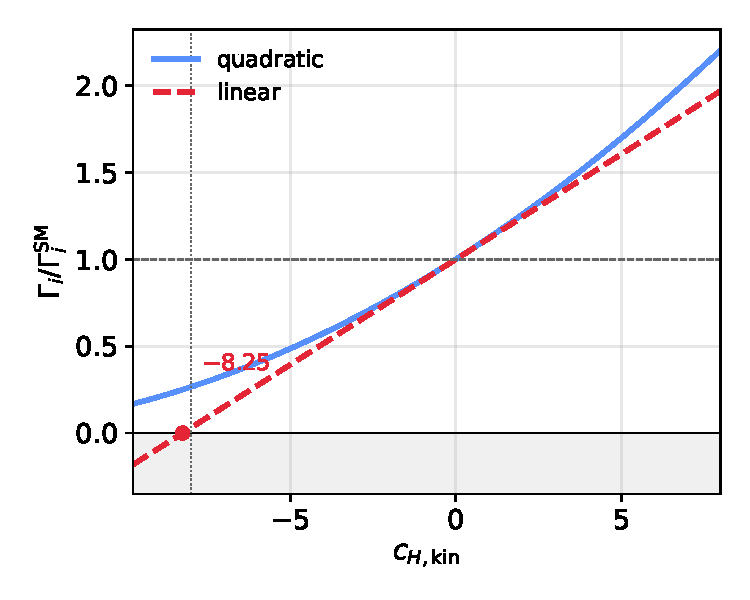
\includegraphics[width=0.49\textwidth]{single_higgs_ch/figures/width_vs_cHkin.pdf}
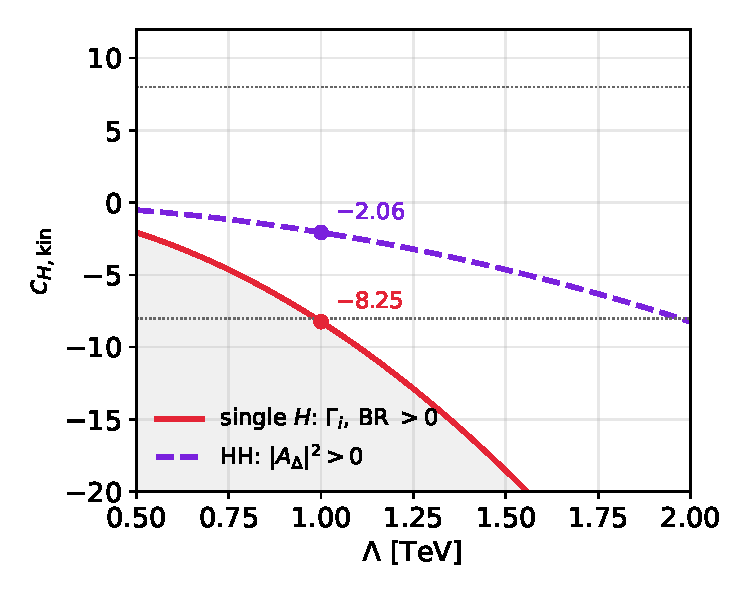
\includegraphics[width=0.49\textwidth]{single_higgs_ch/figures/physical_region_cHkin.pdf}
\caption{Left: single-Higgs partial widths as a function of $c_{\PH\mathrm{kin}}$
at $\Lambda=1$~TeV, Eq.~\eqref{eq:chkinwidth}, in the quadratic (solid) and linear
(dashed) truncations. The grey band marks negative widths, the marker the zero of the
linear form, Eq.~\eqref{eq:chkinzero}, and the dotted line the lower edge of the range
of Table~\ref{tab:SMEFTcouplings}. Right: the lower bound on $c_{\PH\mathrm{kin}}$
for positive linearly truncated rates as a function of $\Lambda$: the single-Higgs
partial widths and branching ratios, Eq.~\eqref{eq:chkinbound} (solid; grey below),
and the \HH triangle-squared term (dashed). The dotted lines mark the range of
Table~\ref{tab:SMEFTcouplings}, the markers the two bounds at $\Lambda=1$~TeV.}
\label{fig:sh_physical}
\end{figure}


\clearpage
\section{Running of the Wilson coefficients}
\label{sec:rge}

The parameterization of Sec.~\ref{sec:parameterization} treats the Wilson coefficients as
constants. They are supplied to the generator at a fixed input scale, $\mu_0 = 173$~GeV,
and the matrix element uses that value at every phase-space point. In the SMEFT the
coefficients run, and a calculation that resums the associated logarithms evaluates them
at a scale characteristic of the process, which for \HH production grows with \mHH. Like
the validity statements of Sec.~\ref{sec:truncation}, this is a property of
Eq.~\eqref{eq:smeftpara_reorg} and not of any analysis selection.

Five of the nine coefficients evolve --- $c_{\PQt\PH}$, $c_{\PH G}$, $c_{\PQt G}$,
$c_{Q\PQt}^{(1)}$ and $c_{Q\PQt}^{(8)}$ --- while the purely bosonic $c_{\PH\Box}$,
$c_{\PH D}$ and $c_\PH$ do not. The subleading coefficients evolve multiplicatively from
their input values, so the operator mixings $c_{Q\PQt}^{(1,8)} \to c_{\PQt\PH}$ and
$c_{\PQt G}, c_{Q\PQt}^{(1,8)} \to c_{\PH G}$ vanish at a point where the subleading
coefficients do. The anomalous dimensions and their solution are those of
Ref.~\cite{Heinrich:2024rtg}.

The size of the omission is measured on samples generated with the running enabled at
$\sqrt{s}=13.6$~TeV, with $\mu_{\text{EFT}} = \mHH/2$. A benchmark with no running
coefficient is reproduced to $0.02\%$ in rate, which bounds any artefact of the
procedure. At $c_{\PQt\PH}=4$, the largest value of the benchmark set, the rate falls by
$2.9\%$ and $\langle\mHH\rangle$ by $1.5\%$, with a coherent tilt of the spectrum at
$5.8\sigma$ --- soft bins up and hard bins down, as expected when a coefficient runs down
with \mHH --- and the effect falls with $c_{\PQt\PH}$.

The coefficients delivered with this report are therefore defined at $\mu_0 = 173$~GeV
and the templates are built with them fixed there. Where the coefficients that run are
small the difference is below the statistics of the comparison; at the upper end of the
$c_{\PQt\PH}$ range it is a few per cent in rate and about one per cent in the mean of
the spectrum, comparable to the modelling uncertainty of Sec.~\ref{sec:uncertainties} and
with a definite shape rather than a normalization. An interpretation that quotes
coefficients at a different scale, or that combines these results with measurements which
do, should either evolve them explicitly or carry an uncertainty of that size. For the
four coefficients that do not run there is nothing to do.

Evolving them explicitly costs no new simulation. At leading logarithmic accuracy the
solution of the dimension-6 renormalization-group equations is linear in the Wilson
coefficients, $c_i(\mu) = U_{ij}(\mu,\mu_0)\,c_j(\mu_0)$, and a linear map composed with
the quadratic polynomial of Eq.~\eqref{eq:smeftpara_reorg} is again a quadratic
polynomial in the same monomials (Sec.~\ref{sec:rge_generation}); the morphing weights
are polynomials in those same monomials, so the basis delivers the running prediction at
the transformed point with the templates it already has.

The shape moves as well, and by more than the rate where several coefficients run
together: over the benchmark set of Sec.~\ref{sec:trunc_modelling}, extended with three
nine-dimensional points, the mean of the \mHH spectrum shifts by up to $9\%$, the
largest shift being at the point that isolates the gluonic and four-top channels. An
analysis sensitive to the spectrum therefore needs the kinematic description to follow
the running and not only the rate. The implementation of that map, its closure against
the running-enabled samples by both routes, and the benchmarks in which the four-fermion
mixings are active are going to be studied in a follow-up work.




\clearpage
\section{Summary and outlook}
\label{sec:conclusion}
\textcolor{red}{TODO: summary and outlook.}

\textcolor{red}{FOR THE OUTLOOK --- the four-top operators. $c_{QQ\PQt\PQt}$ and
$c_{QQ}^{(8)}$ are in the parameterization because the generated samples cannot be
described without them (Sec.~\ref{sec:validation_ladder}), but after a realistic
selection they are flat: their acceptance varies by less than $0.1$ over the full
generated range in either $4\PQb$ selection, and $c_{Q\PQt}^{(1)}$ and $c_{Q\PQt}^{(8)}$
are degenerate with each other to $20\%$
(Sec.~\ref{sec:validation_subleading_role}). An LHC \HH analysis therefore gains nothing
by floating them and should say which it fixed. Nor does single-\PH data recover
them: being built from third-generation quark fields alone they have no tree-level
single-Higgs vertex, and single-\PH reaches them only through the running mixing of
$c_{Q\PQt}^{(1,8)}$ into $c_{\PQt\PH}$ and $c_{\PH G}$ (Sec.~\ref{sec:rge}) --- which
does not touch $c_{QQ\PQt\PQt}$ and $c_{QQ}^{(8)}$ at all. Their constraint comes from
$\ttbar\ttbar$, as the ranges of Sec.~\ref{sec:grids} already take it. This is a
statement about the LHC, not about the operators: they grow with the momentum transfer,
so at $100$~TeV the same directions may be the ones that carry the information --- to be
tested with the $100$~TeV grid (Sec.~\ref{sec:energy_beyond}), against a
$\ttbar\ttbar$ rate that grows with the energy as well.}

\textcolor{red}{\textbf{MATHEUS, OSCAR:} the place to follow this up is the running.
Two of the five coefficients that evolve are the four-fermion ones
(Sec.~\ref{sec:rge}), and the nine-dimensional benchmarks of Ref.~\cite{HH_SMEFT_RGE}
are the points where their mixings are live. Once the running is on, the question to ask is
whether the mixing of $c_{Q\PQt}^{(1,8)}$ into $c_{\PQt\PH}$ and $c_{\PH G}$ gives an
\HH analysis a handle on a direction its own acceptance is flat in, or whether it only
moves the rate again.}

\textcolor{red}{FOR THE SUMMARY --- why nine coefficients and not five. The four
four-fermion operators are what this report adds to the set used in
Ref.~\cite{Alasfar:2023xpc}, and on the evidence here no \HH selection measures any of
them: $c_{QQ\PQt\PQt}$ and $c_{QQ}^{(8)}$ are flat in both $4\PQb$ selections, and
$c_{Q\PQt}^{(1)}$ and $c_{Q\PQt}^{(8)}$ are degenerate with each other
(Sec.~\ref{sec:validation_subleading_role}). The detour is still worth stating, for two
reasons that are measured rather than asserted. First, the description: evaluated on the
same samples, the forty-term parameterization is the only one that keeps improving where
the four-fermion coefficients are switched on, $1.9\%$ against $2.4\%$, and the same
holds for the basis once its templates are built by reweighting, $2.50\%$ to $2.11\%$
(Sec.~\ref{sec:validation_ladder}). A five-coefficient description fitted in that region
does not fail visibly; it absorbs the missing operators into the coefficients it has.
Second, the running: $c_{Q\PQt}^{(1)}$ and $c_{Q\PQt}^{(8)}$ are two of the five
coefficients that evolve, and their mixing into $c_{\PQt\PH}$ and $c_{\PH G}$ is the only
route by which the running reaches the Higgs operators, so the follow-up of
Ref.~\cite{HH_SMEFT_RGE} is possible only with them in the parameterization. The nine-coefficient
set therefore buys a description that does not have to be trusted outside the region it
was fitted in, and the starting point for the running, rather than nine measured
directions.}


\clearpage
\section*{Acknowledgements}
\textcolor{red}{TODO: acknowledgements.}

\paragraph{Funding information}
This work was supported by ...
Spyridon Merianos is a Postdoctoral Researcher of the Fonds de la Recherche Scientifique -- FNRS.


\begin{appendix}
\numberwithin{equation}{section}

%\section{Full SMEFT parameterization}
\label{sec:appendix_smeft_parameterization}

The same comments applies to the \ggHH process modeled by SMEFT, which can be parameterized in a similar way by the set of coefficients $\mathbf{c}^{\text{SMEFT}}_i=\{c_\PH,c_{\PH kin},c_{\PQt\PH}, c_{\PH G},  c_{\PQt G},\,c_{Q\PQt}^{(1)},c_{Q\PQt}^{(8)},c_{QQ\PQt\PQt},c_{QQ}^{(8)}\}$:
\begin{align}\label{smeftparams}
\notag\frac{d}{d\xi_j}\sigma_{\ggHH}(\mathbf{c}^{\text{SMEFT}}_i)&= A^j_0 + A^j_1\,c_{\text{H}} + A^j_2\,c_{\text{H},\mathrm{kin}} + A^j_3\,c_{\PQt\PH} + A^j_4\,c_{\text{H}G}\\\notag
& + A^j_5\,c_{tG} + A^j_6\,c_{Qt1} + A^j_7\,c_{Qt8}^{} + A^j_8\,c_{QQtt}^{} + A^j_9\,c_{QQ8}\\\notag
& + A^j_{10}\,c_\text{H} c_{\text{H}\mathrm{kin}} + A^j_{11}\,c_\text{H} c_{\PQt\PH} + A^j_{12}\,c_H c_{\text{H}G} + A^j_{13}\,c_\text{H} c_{tG} + A^j_{14}\,c_\text{H} c_{Qt1}\\
& + A^j_{15}\,c_\text{H} c_{Qt8}^{} + A^j_{16}\,c_\text{H} c_{QQtt}^{} + A^j_{17}\,c_\text{H} c_{QQ8} + A^j_{18}\,c_{\text{H}\mathrm{kin}} c_{\PQt\PH}\\\notag
& + A^j_{19}\,c_{\text{H}\mathrm{kin}} c_{\text{H}G} + A^j_{20}\,c_{\text{H}\mathrm{kin}} c_{tG} + A^j_{21}\,c_{\text{H}\mathrm{kin}} c_{Qt1} + A^j_{22}\,c_{\text{H}\mathrm{kin}} c_{Qt8}^{} + A^j_{23}\,c_{\text{H}\mathrm{kin}} c_{QQtt}^{}\\\notag
& + A^j_{24}\,c_{\text{H}\mathrm{kin}} c_{QQ8} + A^j_{25}\,c_{\PQt\PH} c_{\text{H}G} + A^j_{26}\,c_{\PQt\PH} c_{tG} + A^j_{27}\,c_{\PQt\PH} c_{Qt1} + A^j_{28}\,c_{\PQt\PH} c_{Qt8}^{}\\\notag
& + A^j_{29}\,c_{\PQt\PH} c_{QQtt}^{} + A^j_{30}\,c_{\PQt\PH} c_{QQ8} + A^j_{31}\,c_{\text{H}G} c_{tG} + A^j_{32}\,c_{\text{H}G} c_{Qt1} + A^j_{33}\,c_{\text{H}G} c_{Qt8}^{}\\\notag
& + A^j_{34}\,c_{\text{H}G} c_{QQtt}^{} + A^j_{35}\,c_{\text{H}G} c_{QQ8} + A^j_{36}\,c_\text{H}^2 + A^j_{37}\,c_{\text{H}\mathrm{kin}}^2 + A^j_{38}\,c_{\PQt\PH}^2 + A^j_{39}\,c_{\text{H}G}^2 \\\notag
    \label{eq:smeftpara}
\end{align}
The set of dimension-6 operators described in this Lagrangian can be separated into two classes: leading operators, with Wilson coefficients $\{c_{\PH\Box},\,c_{\PH D},\,c_\PH,\,c_{\PQt},\,c_{\PH G}\}$, and subleading, with $\{c_{\PQt G},\,c_{Q\PQt}^{(1)},\,c_{Q\PQt}^{(8)},\,c_{QQ}^{(1)},\,c_{QQ}^{(8)},\,c_{\PQt\PQt}\}$. By "subleading", we intend operators entering only in loop-induced diagrams, hence carrying an implicit loop factor $L=(16\pi^2)^{-1}$. 
This setup considers SM+linear dimension-6+quadratic dimension-6 contributions for leading operators at the cross section level, while subleading operators enter only linearly---therefore, $|\mathcal{M}_{\text{dim6}}^{\text{sublead}}|^2$ is neglected, and only interference terms with the leading part is considered. Furthermore, $c_{QQ}^{(1)}$ and $c_{\PQt\PQt}$ are combined into a single parameter $c_{QQ\PQt\PQt}=c_{QQ}^{(1)}+c_{\PQt\PQt}$, as their contributions to the amplitude can be factorized.

\begin{table}[h]
\centering
\renewcommand{\arraystretch}{1.2}
\begin{tabular}{cc|cc|cc|cc}
\hline
$\widetilde{A}^j_k$ & $A^j_m$ & $\widetilde{A}^j_k$ & $A^j_m$ & $\widetilde{A}^j_k$ & $A^j_m$ & $\widetilde{A}^j_k$ & $A^j_m$ \\
\hline
0 & 0 & 1 & 1 & 2 & 2 & 3 & 3 \\
4 & 4 & 5 & 36 & 6 & 10 & 7 & 11 \\
8 & 12 & 9 & 37 & 10 & 18 & 11 & 19 \\
12 & 38 & 13 & 25 & 14 & 39 & 15 & 5 \\
16 & 6 & 17 & 7 & 18 & 8 & 19 & 9 \\
20 & 13 & 21 & 14 & 22 & 15 & 23 & 16 \\
24 & 17 & 25 & 20 & 26 & 21 & 27 & 22 \\
28 & 23 & 29 & 24 & 30 & 26 & 31 & 27 \\
32 & 28 & 33 & 29 & 34 & 30 & 35 & 31 \\
36 & 32 & 37 & 33 & 38 & 34 & 39 & 35 \\
\hline
\end{tabular}
\caption{Translation between the renumbered coefficients $\widetilde{A}^j_k$ of the rearranged parameterization in Eq.~\eqref{eq:smeftpara_reorg} and the original coefficients $A^j_m$ of Eq.~\eqref{smeftparams}.}
\label{tab:smeft_index_translation}
\end{table}


%\section{Basis parametrization}
\label{sec:appendix_basis_parametrization}

To reduce the dimensionality of the basis search, and to give the basis a canonical ordering, each basis point is constrained so that it maps onto exactly one coupling combination of Eq.~\eqref{eq:smeftpara_reorg}. The resulting minimal basis has the form:

\begin{multline}\Bigl[ \begin{bmatrix} 0, & 0, & 0, & 0, & 0, & 0, & 0, & 0, & 0  \end{bmatrix},\,
 \begin{bmatrix} A_{1}, & 0, & 0, & 0, & 0, & 0, & 0, & 0, & 0  \end{bmatrix},\, \\ %c_H
 \begin{bmatrix} 0, & A_{2}, & 0, & 0, & 0, & 0, & 0, & 0, & 0  \end{bmatrix},\, % c_{K,kin}
 \begin{bmatrix} 0, & 0, & A_{3}, & 0, & 0, & 0, & 0, & 0, & 0  \end{bmatrix},\, \\ % c_{tH}
 \begin{bmatrix} 0, & 0, & 0, & A_{4}, & 0, & 0, & 0, & 0, & 0  \end{bmatrix},\, % c_{HG}
 \begin{bmatrix} 0, &  0, & 0, &  0, & A_{5}, & 0, & 0, & 0, & 0  \end{bmatrix},\, \\% c_{tG}
 \begin{bmatrix} 0, &  0, &  0, &  0, & 0, & A_{6}, & 0, & 0, & 0  \end{bmatrix},\,  %c_{Qt}
 \begin{bmatrix} 0, &  0, &  0, &  0, & 0, & 0, & A_{7}, & 0, & 0  \end{bmatrix},\, \\% c_{Qt8}
 \begin{bmatrix} 0, &  0, &  0, &  0, & 0, & 0, & 0, & A_{8}, & 0  \end{bmatrix},\,  %c_{QQtt}
 \begin{bmatrix} 0, &  0, &  0, &  0, & 0, & 0, & 0, & 0, & A_{9}  \end{bmatrix},\, \\ % c_{QQ8}
 \begin{bmatrix} A_{10}, & 0, & 0, & 0, & 0, & 0, & 0, & 0, & 0  \end{bmatrix},\, %c_H^2
 \begin{bmatrix} A_{11a}, & A_{11b}, & 0, & 0, & 0, & 0, & 0, & 0, & 0  \end{bmatrix},\, \\ %c_{H}c_{Hkin}
 \begin{bmatrix} A_{12a}, & 0, & A_{12b}, & 0, & 0, & 0, & 0, & 0, & 0  \end{bmatrix},\, % c_{H}c_{tH}
 \begin{bmatrix} A_{13a}, & 0, & 0, & A_{13b}, & 0, & 0, & 0, & 0, & 0  \end{bmatrix},\, \\ %c_{H}c_{HG}
 \begin{bmatrix} 0, & A_{14}, & 0, & 0, & 0, & 0, & 0, & 0, & 0  \end{bmatrix},\, % c_{H,kin}^2
 \begin{bmatrix} 0, &  A_{15a}, & A_{15b}, & 0, & 0, & 0, & 0, & 0, & 0  \end{bmatrix},\, \\% c_{Hkin}c_{uH}
 \begin{bmatrix} 0, &  A_{16a}, & 0, & A_{16b}, & 0, & 0, & 0, & 0, & 0  \end{bmatrix},\,  %c_{Hkin}c_{HG}
 \begin{bmatrix} 0, & 0, & A_{17}, & 0, & 0, & 0, & 0, & 0, & 0  \end{bmatrix},\, \\ %c_{tH}^2
\begin{bmatrix} 0, & 0, &  A_{18a}, & A_{18b}, & 0, & 0, & 0, & 0, & 0  \end{bmatrix},\,  %c_{tH}c_{HG}
 \begin{bmatrix} 0, & 0, & 0, & A_{19}, & 0, & 0, & 0, & 0, & 0  \end{bmatrix},\, \\ % c_{Hg}^2
 \begin{bmatrix} A_{20a}, & 0, & 0, & 0, & A_{20b}, & 0, & 0, & 0, & 0  \end{bmatrix},\, % c_{H}c_{tG}
 \begin{bmatrix} A_{21a}, & 0, & 0, & 0, & 0, & A_{21b}, & 0, & 0, & 0  \end{bmatrix},\, \\ %c_{H}c_{Qt}
 \begin{bmatrix} A_{22a}, & 0, & 0, & 0, & 0, & 0, & A_{22b}, & 0, & 0  \end{bmatrix},\, % c_{H}c_{Qt8}
 \begin{bmatrix} A_{23a}, & 0, & 0, & 0, & 0, & 0, & 0, & A_{23b}, & 0  \end{bmatrix},\, \\ %c_{H}c_{QQtt}
 \begin{bmatrix} A_{24a}, & 0, & 0, & 0, & 0, & 0, & 0, & 0, & A_{24b}  \end{bmatrix},\, % c_{H}c_{QQ8}
 \begin{bmatrix} 0, &  A_{25a}, & 0, & 0, & A_{25b}, & 0, & 0, & 0, & 0  \end{bmatrix},\, \\% c_{Hkin}c_{tG}
 \begin{bmatrix} 0, &  A_{26a}, & 0, & 0, & 0, & A_{26b}, & 0, & 0, & 0  \end{bmatrix},\,  %c_{Hkin}c_{Qt}
 \begin{bmatrix} 0, &  A_{27a}, & 0, & 0, & 0, & 0, & A_{27b}, & 0, & 0  \end{bmatrix},\, \\% c_{Hkin}c_{Qt8}
 \begin{bmatrix} 0, &  A_{28a}, & 0, & 0, & 0, & 0, & 0, & A_{28b}, & 0  \end{bmatrix},\,  %c_{Hkin}c_{QQtt}
 \begin{bmatrix} 0, &  A_{29a}, & 0, & 0, & 0, & 0, & 0, & 0, & A_{29b}  \end{bmatrix},\, \\% c_{Hkin}c_{QQ8}
 \begin{bmatrix} 0, &  0, &  A_{30a}, & 0, & A_{30b}, & 0, & 0, & 0, & 0  \end{bmatrix},\, % c_{tH}c_{tG}
 \begin{bmatrix} 0, &  0, &  A_{31a}, & 0, & 0, & A_{31b}, & 0, & 0, & 0  \end{bmatrix},\, \\  %c_{tH}c_{Qt}
 \begin{bmatrix} 0, &  0, &  A_{32a}, & 0, & 0, & 0, & A_{32b}, & 0, & 0  \end{bmatrix},\, % c_{tH}c_{Qt8}
 \begin{bmatrix} 0, &  0, &  A_{33a}, & 0, & 0, & 0, & 0, & A_{33b}, & 0  \end{bmatrix},\, \\ %c_{tH}c_{QQtt}
 \begin{bmatrix} 0, &  0, &  A_{34a}, & 0, & 0, & 0, & 0, & 0, & A_{34b}  \end{bmatrix},\, % c_{tH}c_{QQ8}
 \begin{bmatrix} 0, &  0, & 0, &  A_{35a}, & A_{35b}, & 0, & 0, & 0, & 0  \end{bmatrix},\, \\% c_{HG}c_{tG}
 \begin{bmatrix} 0, &  0, &  0, &  A_{36a}, & 0, & A_{36b}, & 0, & 0, & 0  \end{bmatrix},\,  %c_{HG}c_{Qt}
 \begin{bmatrix} 0, &  0, &  0, &  A_{37a}, & 0, & 0, & A_{37b}, & 0, & 0  \end{bmatrix},\, \\% c_{HG}c_{Qt8}
 \begin{bmatrix} 0, &  0, &  0, &  A_{38a}, & 0, & 0, & 0, & A_{38b}, & 0  \end{bmatrix},\,  %c_{HG}c_{QQtt}
 \begin{bmatrix} 0, &  0, &  0, &  A_{39a}, & 0, & 0, & 0, & 0, & A_{39b}  \end{bmatrix},\, % c_{HG}c_{QQ8}
\Bigl] 
\end{multline}
with each basis point parametrized as $\begin{bmatrix} c_\PH, &  c_{\PH,kin}, &  c_{\PQt\PH}, & c_{\PH G}, & c_{\PQt G}, & c_{Q\PQt}^{(1)}, & c_{Q \PQt}^{(8)}, & c_{QQ\PQt\PQt}, & c_{QQ}^{(8)} \end{bmatrix}$

with each basis point in the form of $\begin{bmatrix} c_\PH, & c_{\PH \mathrm{kin}}, & c_{\PQt\PH}, & c_{\PH G}, & c_{\PQt G}, & c_{Q\PQt}^{(1)}, & c_{Q\PQt}^{(8)}, & c_{QQ\PQt\PQt}, & c_{QQ}^{(8)} \end{bmatrix}$.

\textcolor{red}{TODO: this skeleton was carried over from the HEFT study; check the ordering against the coupling combinations actually used in Eq.~\eqref{eq:smeftpara_reorg}.}


\clearpage
%\section{Validation samples}
\label{sec:appendix_samples}

\textcolor{red}{TODO: list the 50 held-out SMEFT samples (25 from the 2D grids and 25 from the 9D Gaussian) with their Wilson coefficient values.}

\section{ELR validation including the four-fermion parameter space}
\label{sec:9dvalidation}
Fifty test-samples with all nine coefficients varying are separated for further validation of the full parameter space. Reasonable modeling is found in all regions. 
\begin{figure}[h!]
  \begin{minipage}[b]{0.495\linewidth}
    \centering
    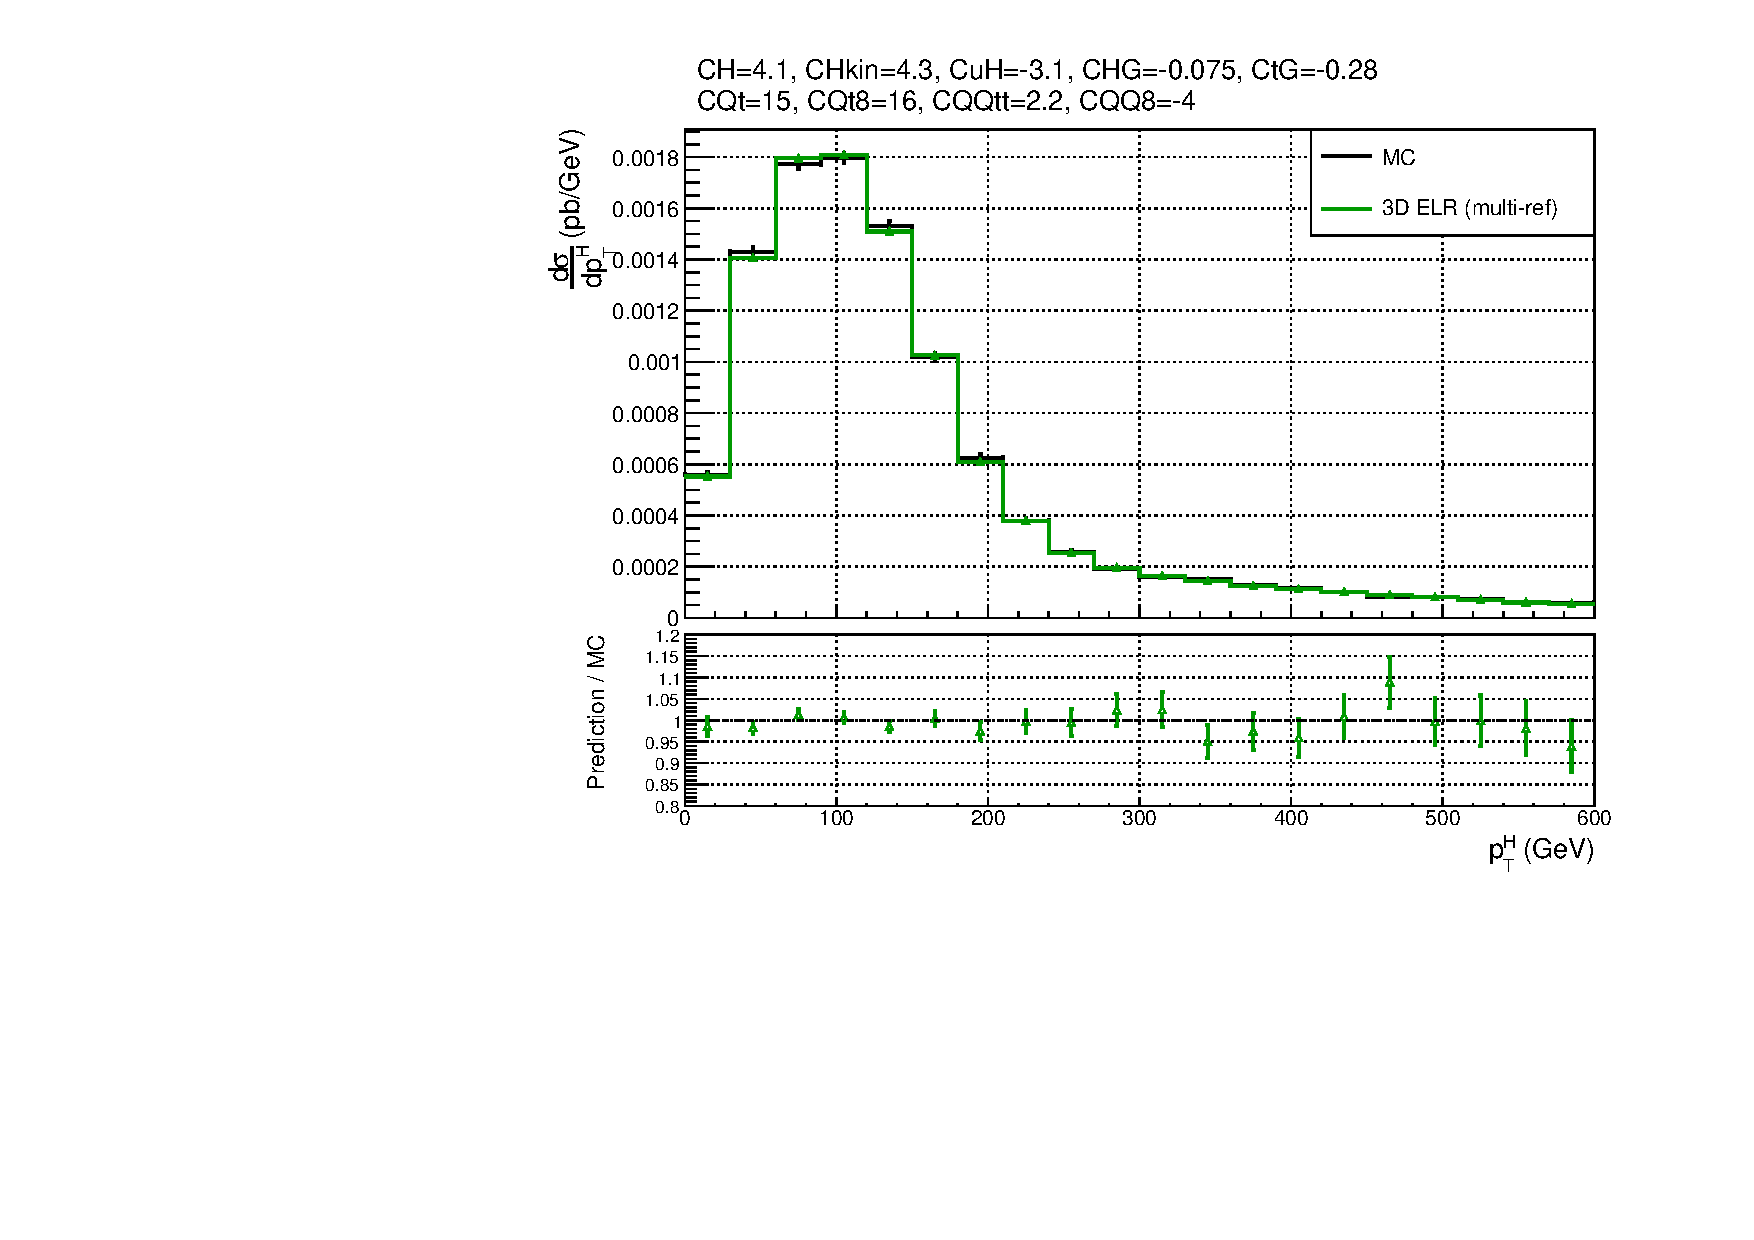
\includegraphics[width=\linewidth]{plots/pth_3d_multiref_(48)_CH_4.13477_CHbox_4.34845_CuH_-3.1115_CHG_-0.0753981_CtG_-0.282248_CQt_15.0718_CQt8_15.8966_CQQtt_2.22505_CQQ8_-3.9732.pdf}
  \end{minipage}
  \hfill
  \begin{minipage}[b]{0.495\linewidth}
    \centering
    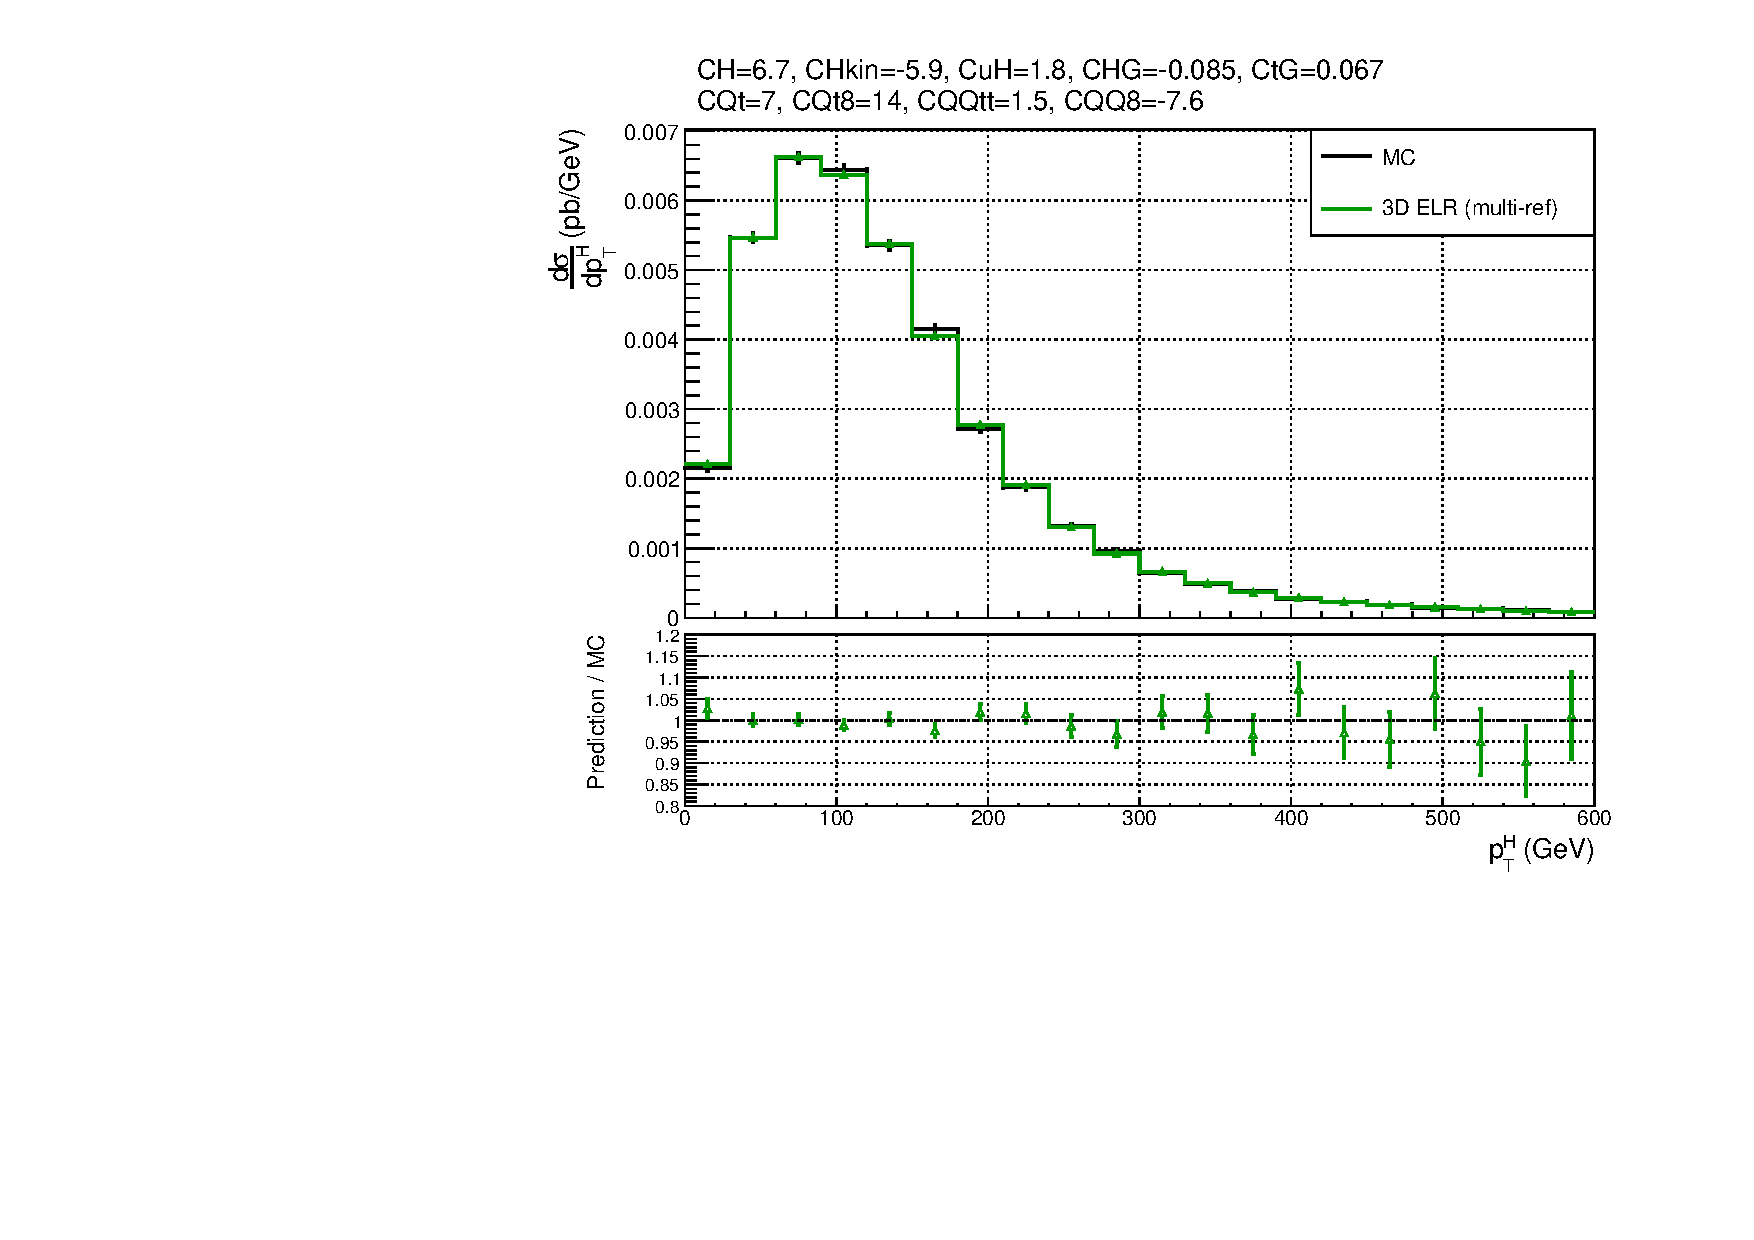
\includegraphics[width=\linewidth]{plots/pth_3d_multiref_(49)_CH_6.67517_CHbox_-5.89157_CuH_1.83813_CHG_-0.0845237_CtG_0.0674596_CQt_7.02121_CQt8_13.5041_CQQtt_1.45086_CQQ8_-7.61857.pdf}
  \end{minipage}
  \caption{Higgs transverse momenta distributions for some of the 9D test-samples generated at $\sqrt{s}=13.6$ TeV.}
  \label{fig:pth3}
\end{figure}
\begin{figure}[h!]
    \centering    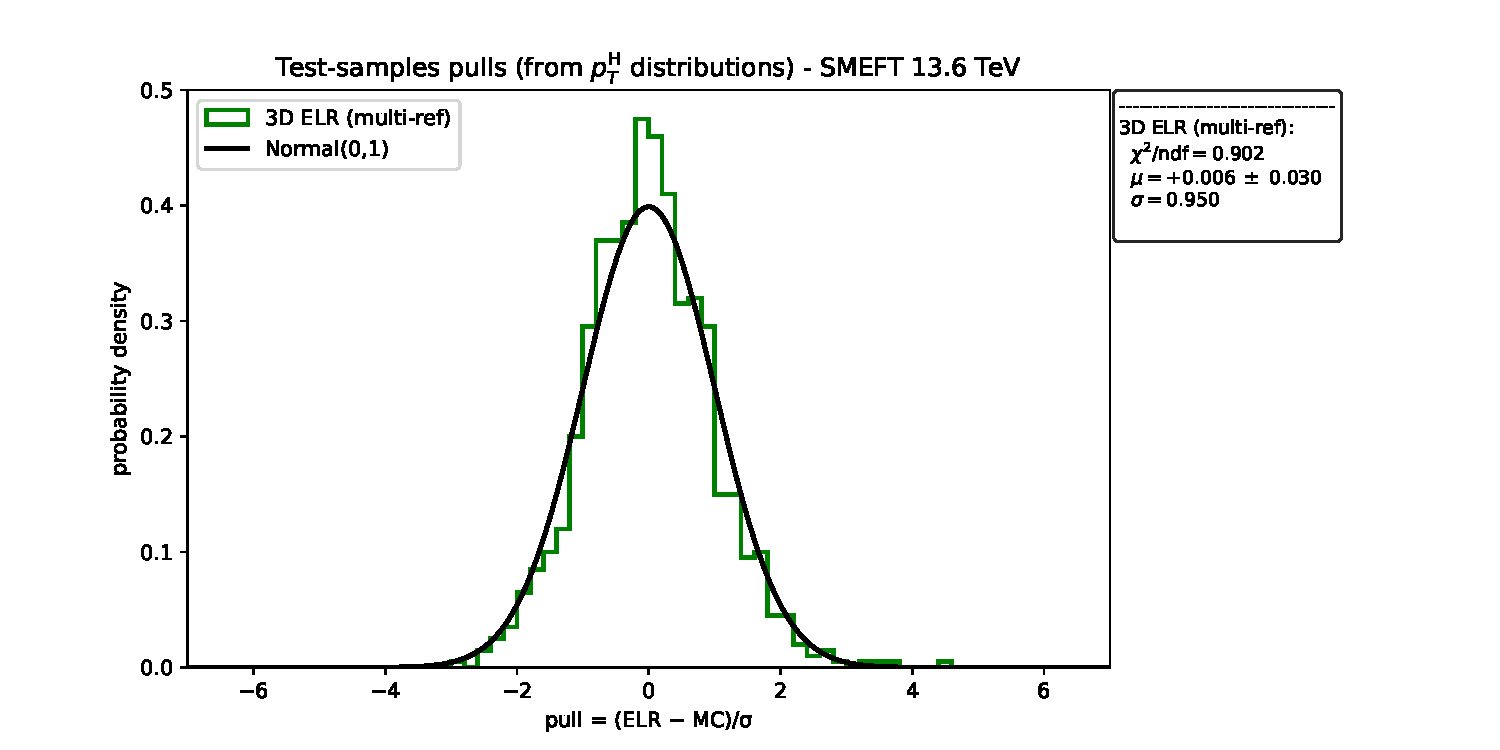
\includegraphics[width=1\linewidth]{plots/stats3.pdf}
    \caption{Pulls and statistical parameters obtained from $p^\text{H}_T$ bins in SMEFT with test-samples varying all the nine coefficients.}
    \label{fig:stats3}
\end{figure}
%\textcolor{red}{TODO: list the 50 held-out SMEFT samples (25 from the 2D grids and 25 from the 9D Gaussian) with their Wilson coefficient values.}

\section{Validation of the $A$-coefficients consistent with \texttt{PDF4LHC21\_40} and at $\sqrt{s}=13$ and $14$ TeV}
\label{sec:validation_transport}
%The transport $K$-factors needed for the coefficients at $13$ and $14$ TeV are obtained with the generation at both COM energies of all basis points in the full 9D-basis shown in Table~\ref{tab:smeft_basis_9d}. The factors are then obtained by using the coefficients obtained through the fit made at $13.6$ TeV to predict the distributions in all bins for all basis points, and then extracting the differences that correct for the MC distributions at $13$ and $14$ TeV. 

\begin{figure}[h!]
    \centering    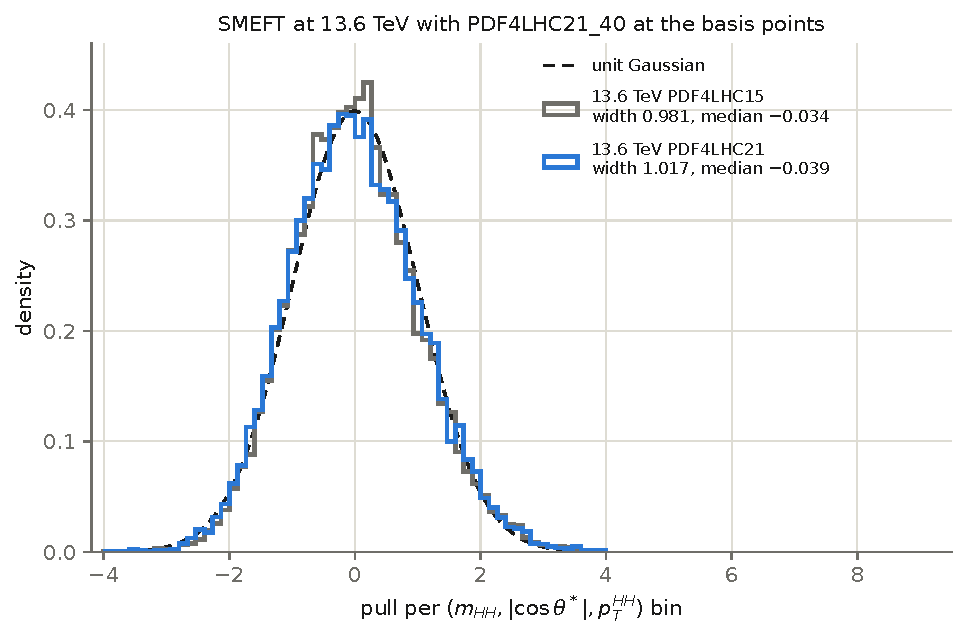
\includegraphics[width=0.8\linewidth]{plots/SMEFT_pulls_13p6TeV_PDF4LHC15_vs_PDF4LHC21.pdf}
    \caption{Pull of the PDF-transported $A$-coefficients per $(\mHH, |\cos\theta^*|, \pt^{HH})$ bin, on the basis points, against a unit Gaussian (dashed). The gray distribution correspond to the coefficients consistent with \texttt{PDF4LHC15} and applied to the basis generated at the same PDF set. Similarly, the blue distribution correspond to the coefficients consistent with \texttt{PDF4LHC21} and applied to the basis points generated at the same PDF set.}
    \label{fig:PDFchange}
\end{figure}
\begin{figure}[h!]
    \centering    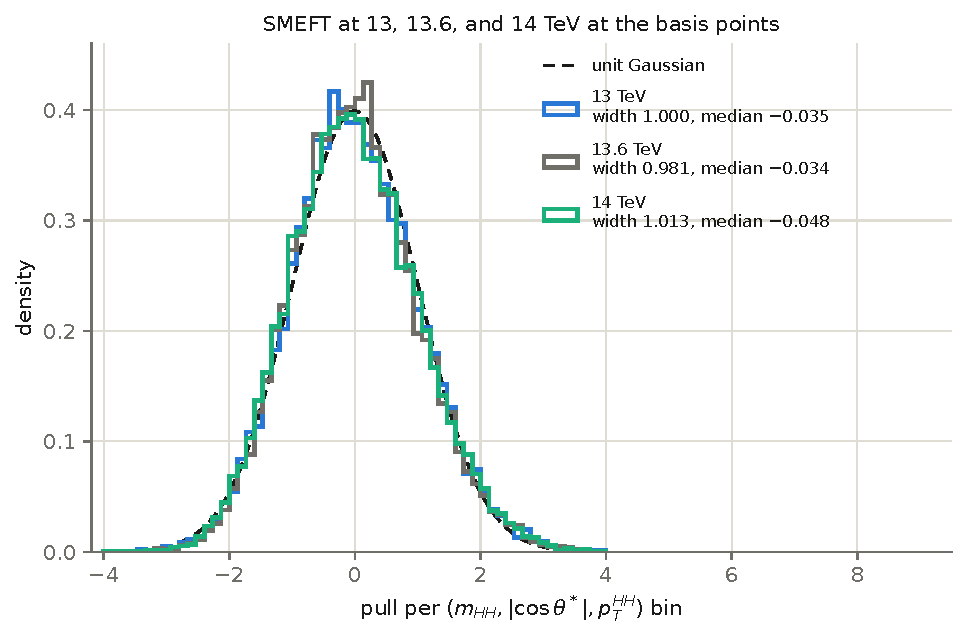
\includegraphics[width=0.8\linewidth]{plots/SMEFT_pulls_13_13p6_14TeV.pdf}
    \caption{Pull of the transported $A$-coefficients per $(\mHH, |\cos\theta^*|, \pt^{HH})$ bin, on the basis points, against a unit Gaussian (dashed).}
    \label{fig:COMEchange}
\end{figure}

In order to validate the transported coefficients, additional samples are generated at the basis points (see Table \ref{tab:smeft_basis_9d}) with the PDF set \texttt{PDF4LHC21\_40} and at $\sqrt{s}=13$ and $14$ TeV. The effects of the PDF change is observed in Figure \ref{fig:PDFchange}, where gaussian-like properties are observed in both the pull distributions, indicating consistent modeling for each of the PDF sets. Finally, the results with all COM energies are exhibited in Figure~\ref{fig:COMEchange}. By comparing the $13.6$ TeV results (fitted coefficients) with the other COM energies (transported coefficients), the same level of agreement is observed. %Figure \ref{fig:pth2} shows some distributions using ELR at both COM energies.

%\begin{figure}[h!]
%    \centering    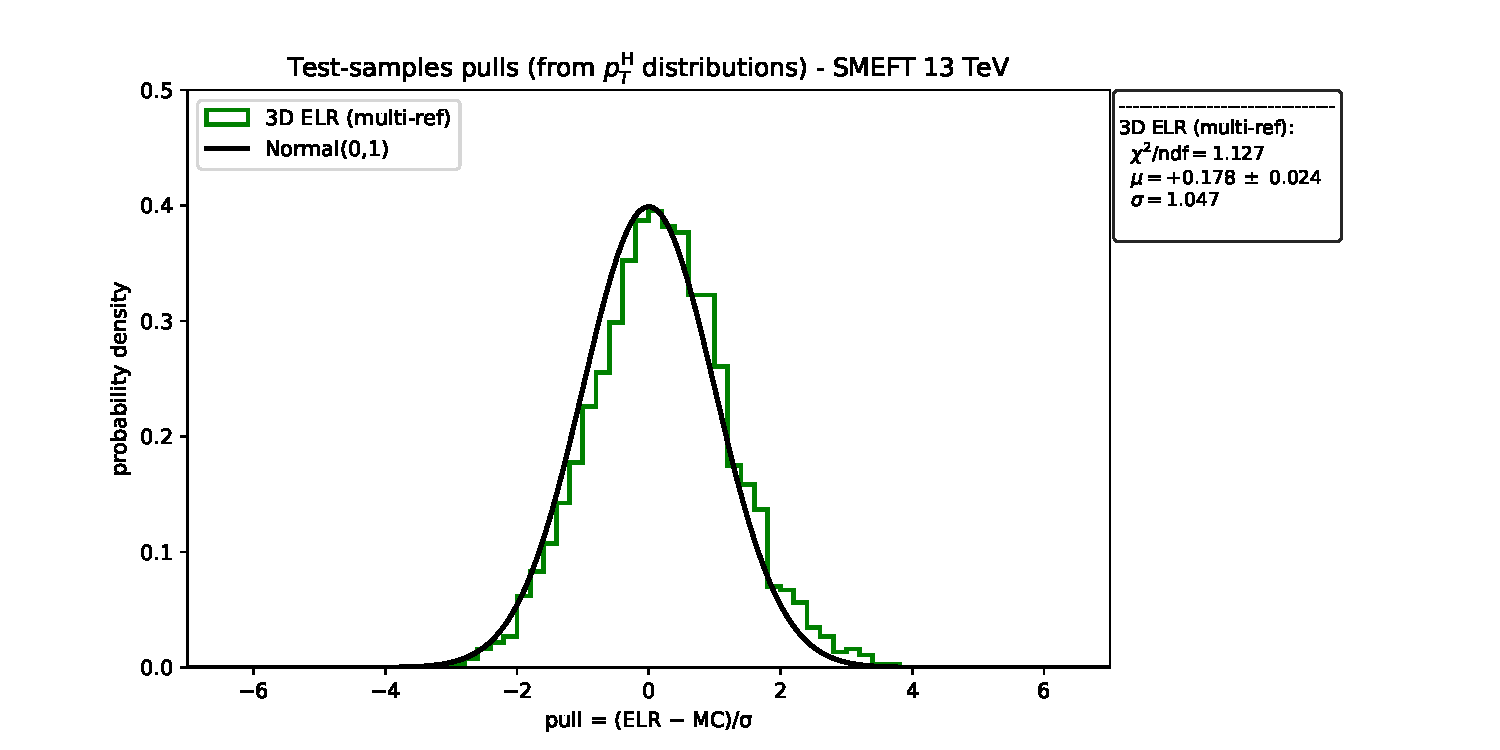
\includegraphics[width=1\linewidth]{plots/pulls_pth_3d_SMEFT13TeV_transport_pt500_plot_2.pdf}
%    \caption{Pulls obtained with all test-samples in all $p^\text{H}_T$ bins in SMEFT. The statistical parameters $\{\chi^2,\mu,\sigma\}$ are very similar to those at obtained at $13.6$ TeV (see Fig.~\ref{fig:stats}), therefore validating the transport among coefficients in different COM energies.}
%    \label{fig:stats2}
%\end{figure}

%\begin{figure}[h!]
%  \begin{minipage}[b]{0.495\linewidth}
%    \centering
%    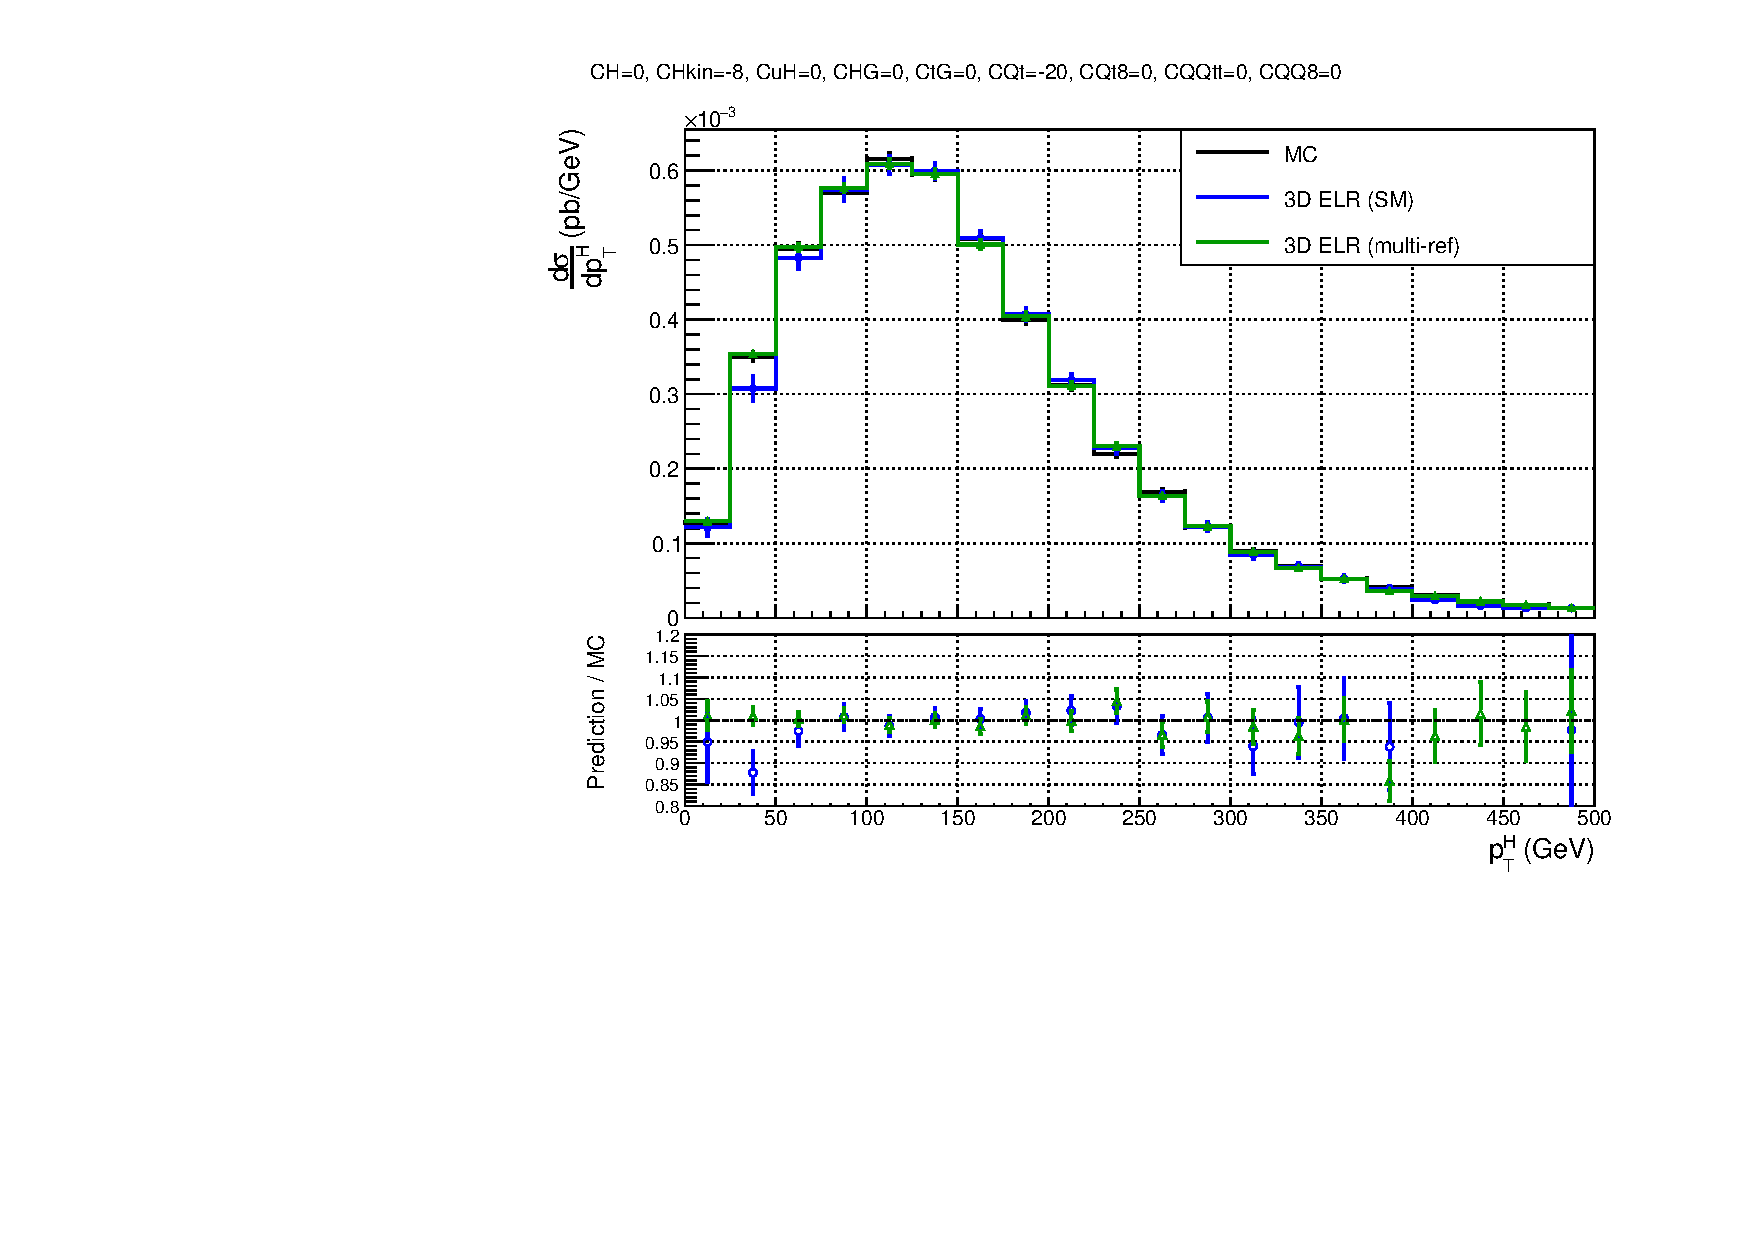
\includegraphics[width=\linewidth]{plots/pth_3d_9D_13TeV_transport_27_CH_0.0_CHbox_-8.0_CuH_0.0_CHG_0.0_CtG_0.0_CQt_-20.0_CQt8_0.0_CQQtt_0.0_CQQ8_0.0.pdf}
%  \end{minipage}
%  \hfill
%  \begin{minipage}[b]{0.495\linewidth}
%    \centering
%    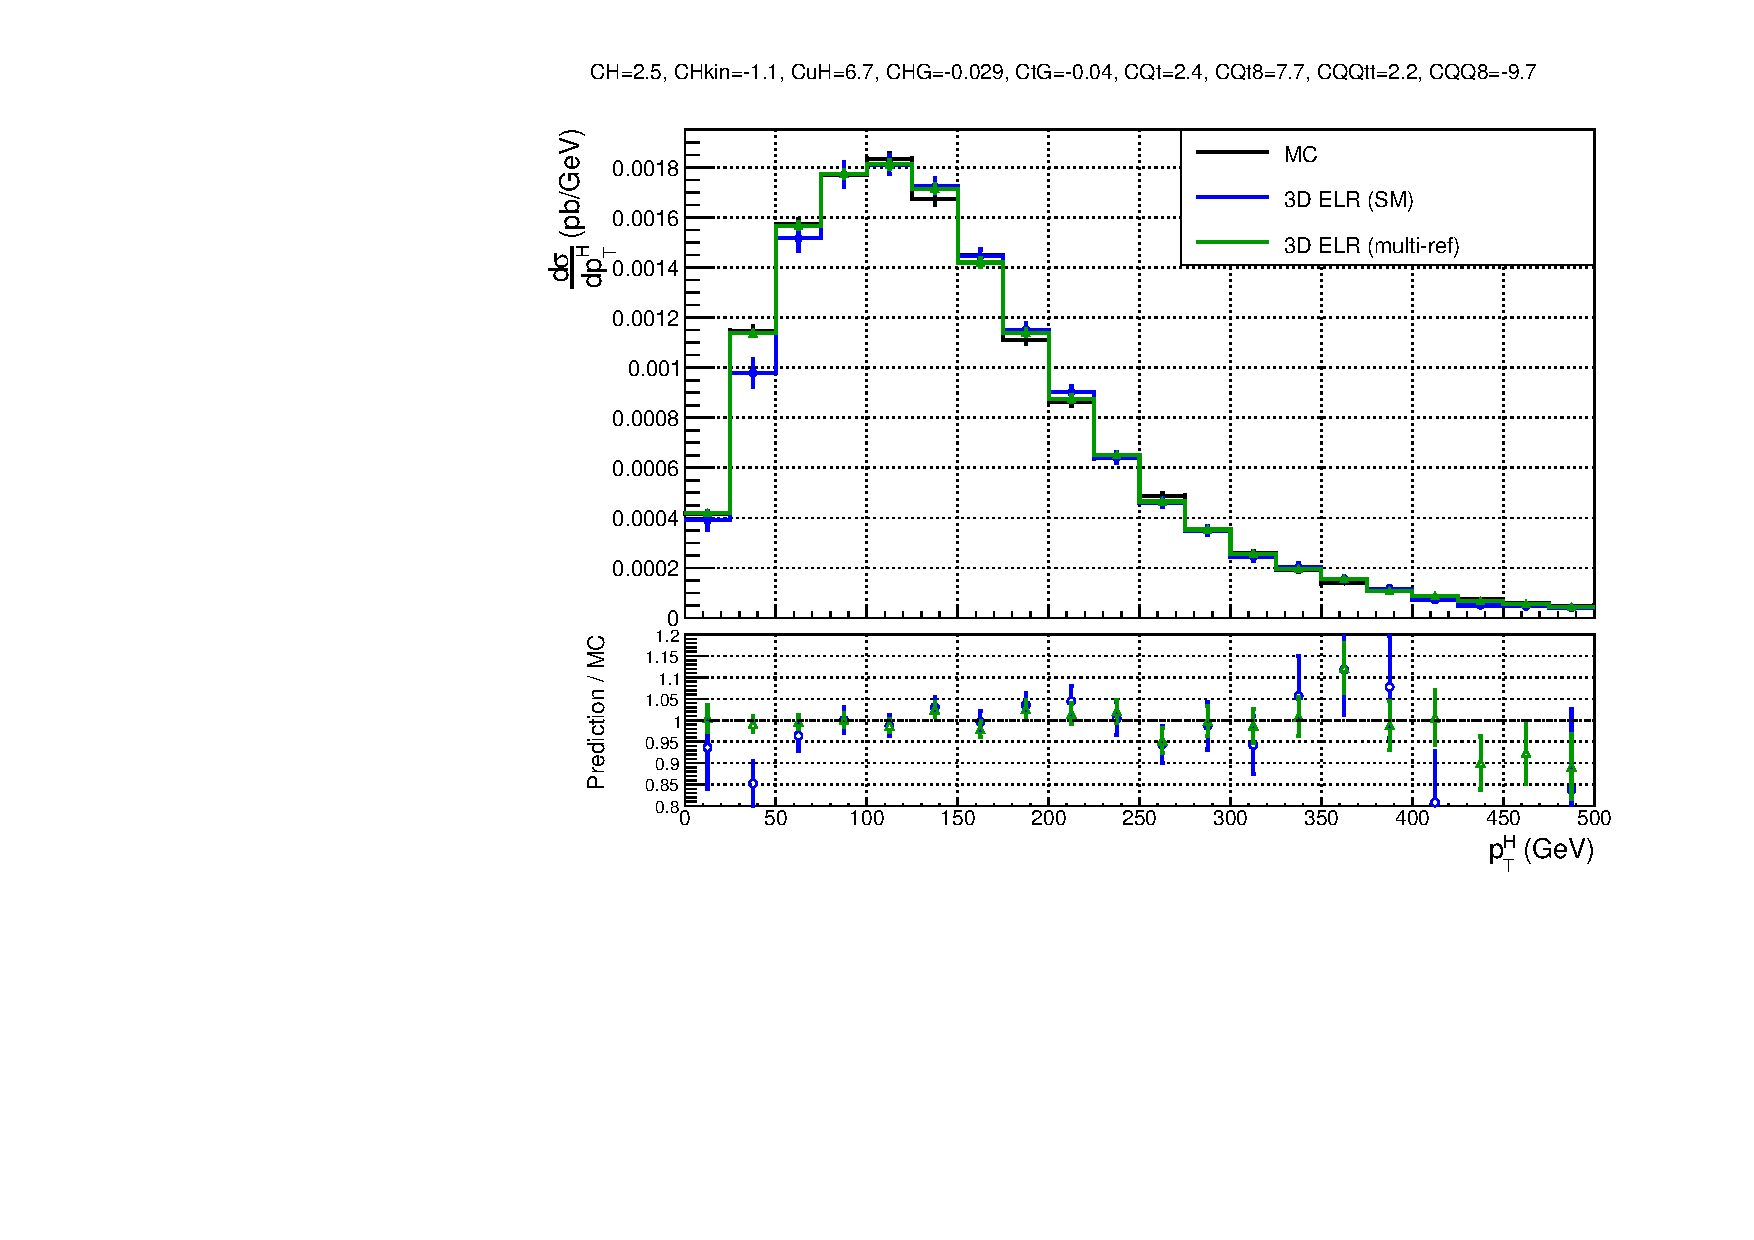
\includegraphics[width=\linewidth]{plots/pth_13TeV_transport_72_CH_2.48_CHbox_-1.12_CuH_6.66_CHG_-0.029_CtG_-0.040_CQt_2.3_CQt8_7.66_CQQtt_2.16_CQQ8_-9.69282.pdf}
%  \end{minipage}
%  \caption{Higgs transverse momenta distributions for some of the test-samples generated at $\sqrt{s}=13$ TeV. The closure is very similar to the case at $13.6$ TeV.}
%  \label{fig:pth2}
%\end{figure}
%\begin{figure}[h!]
%  \centering
  % First group: 2 x 2
%  \begin{minipage}[b]{0.495\linewidth}
%    \centering
    %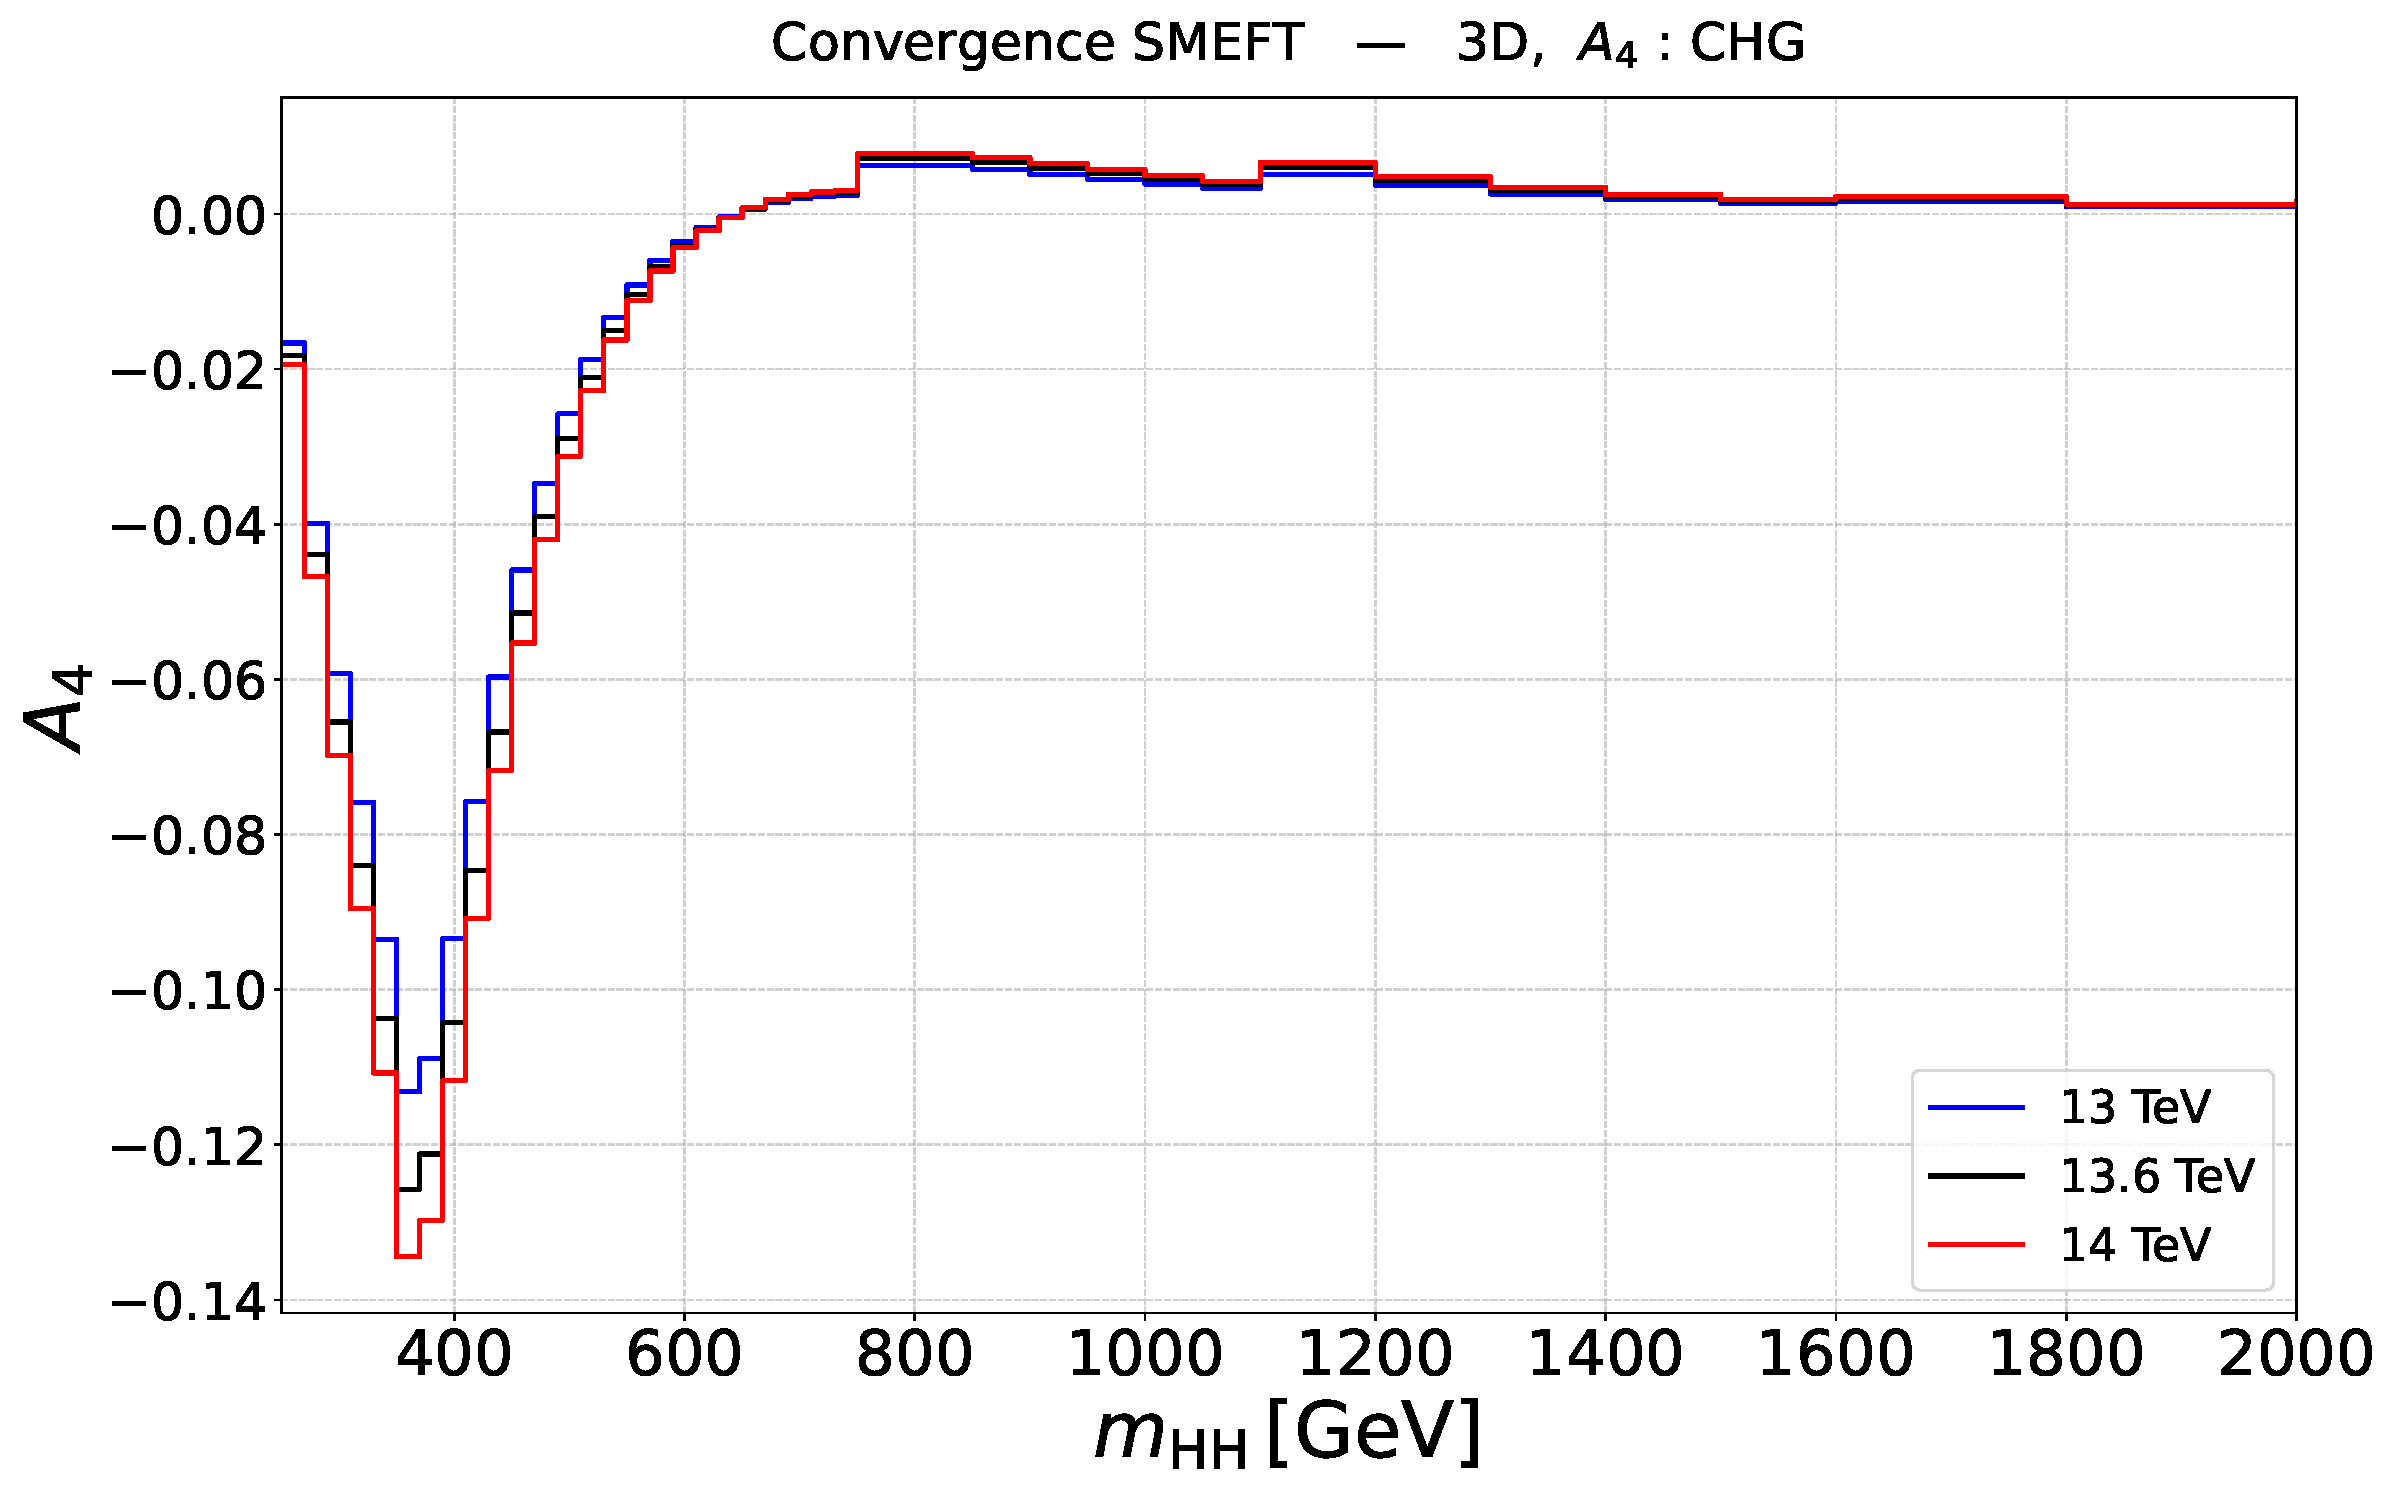
\includegraphics[width=\linewidth]{plots/plot_param4_250_2000_3d_energy_13_13p6_14TeV.pdf}
  %\end{minipage}
  %\hfill
  %\begin{minipage}[b]{0.495\linewidth}
   % \centering
    %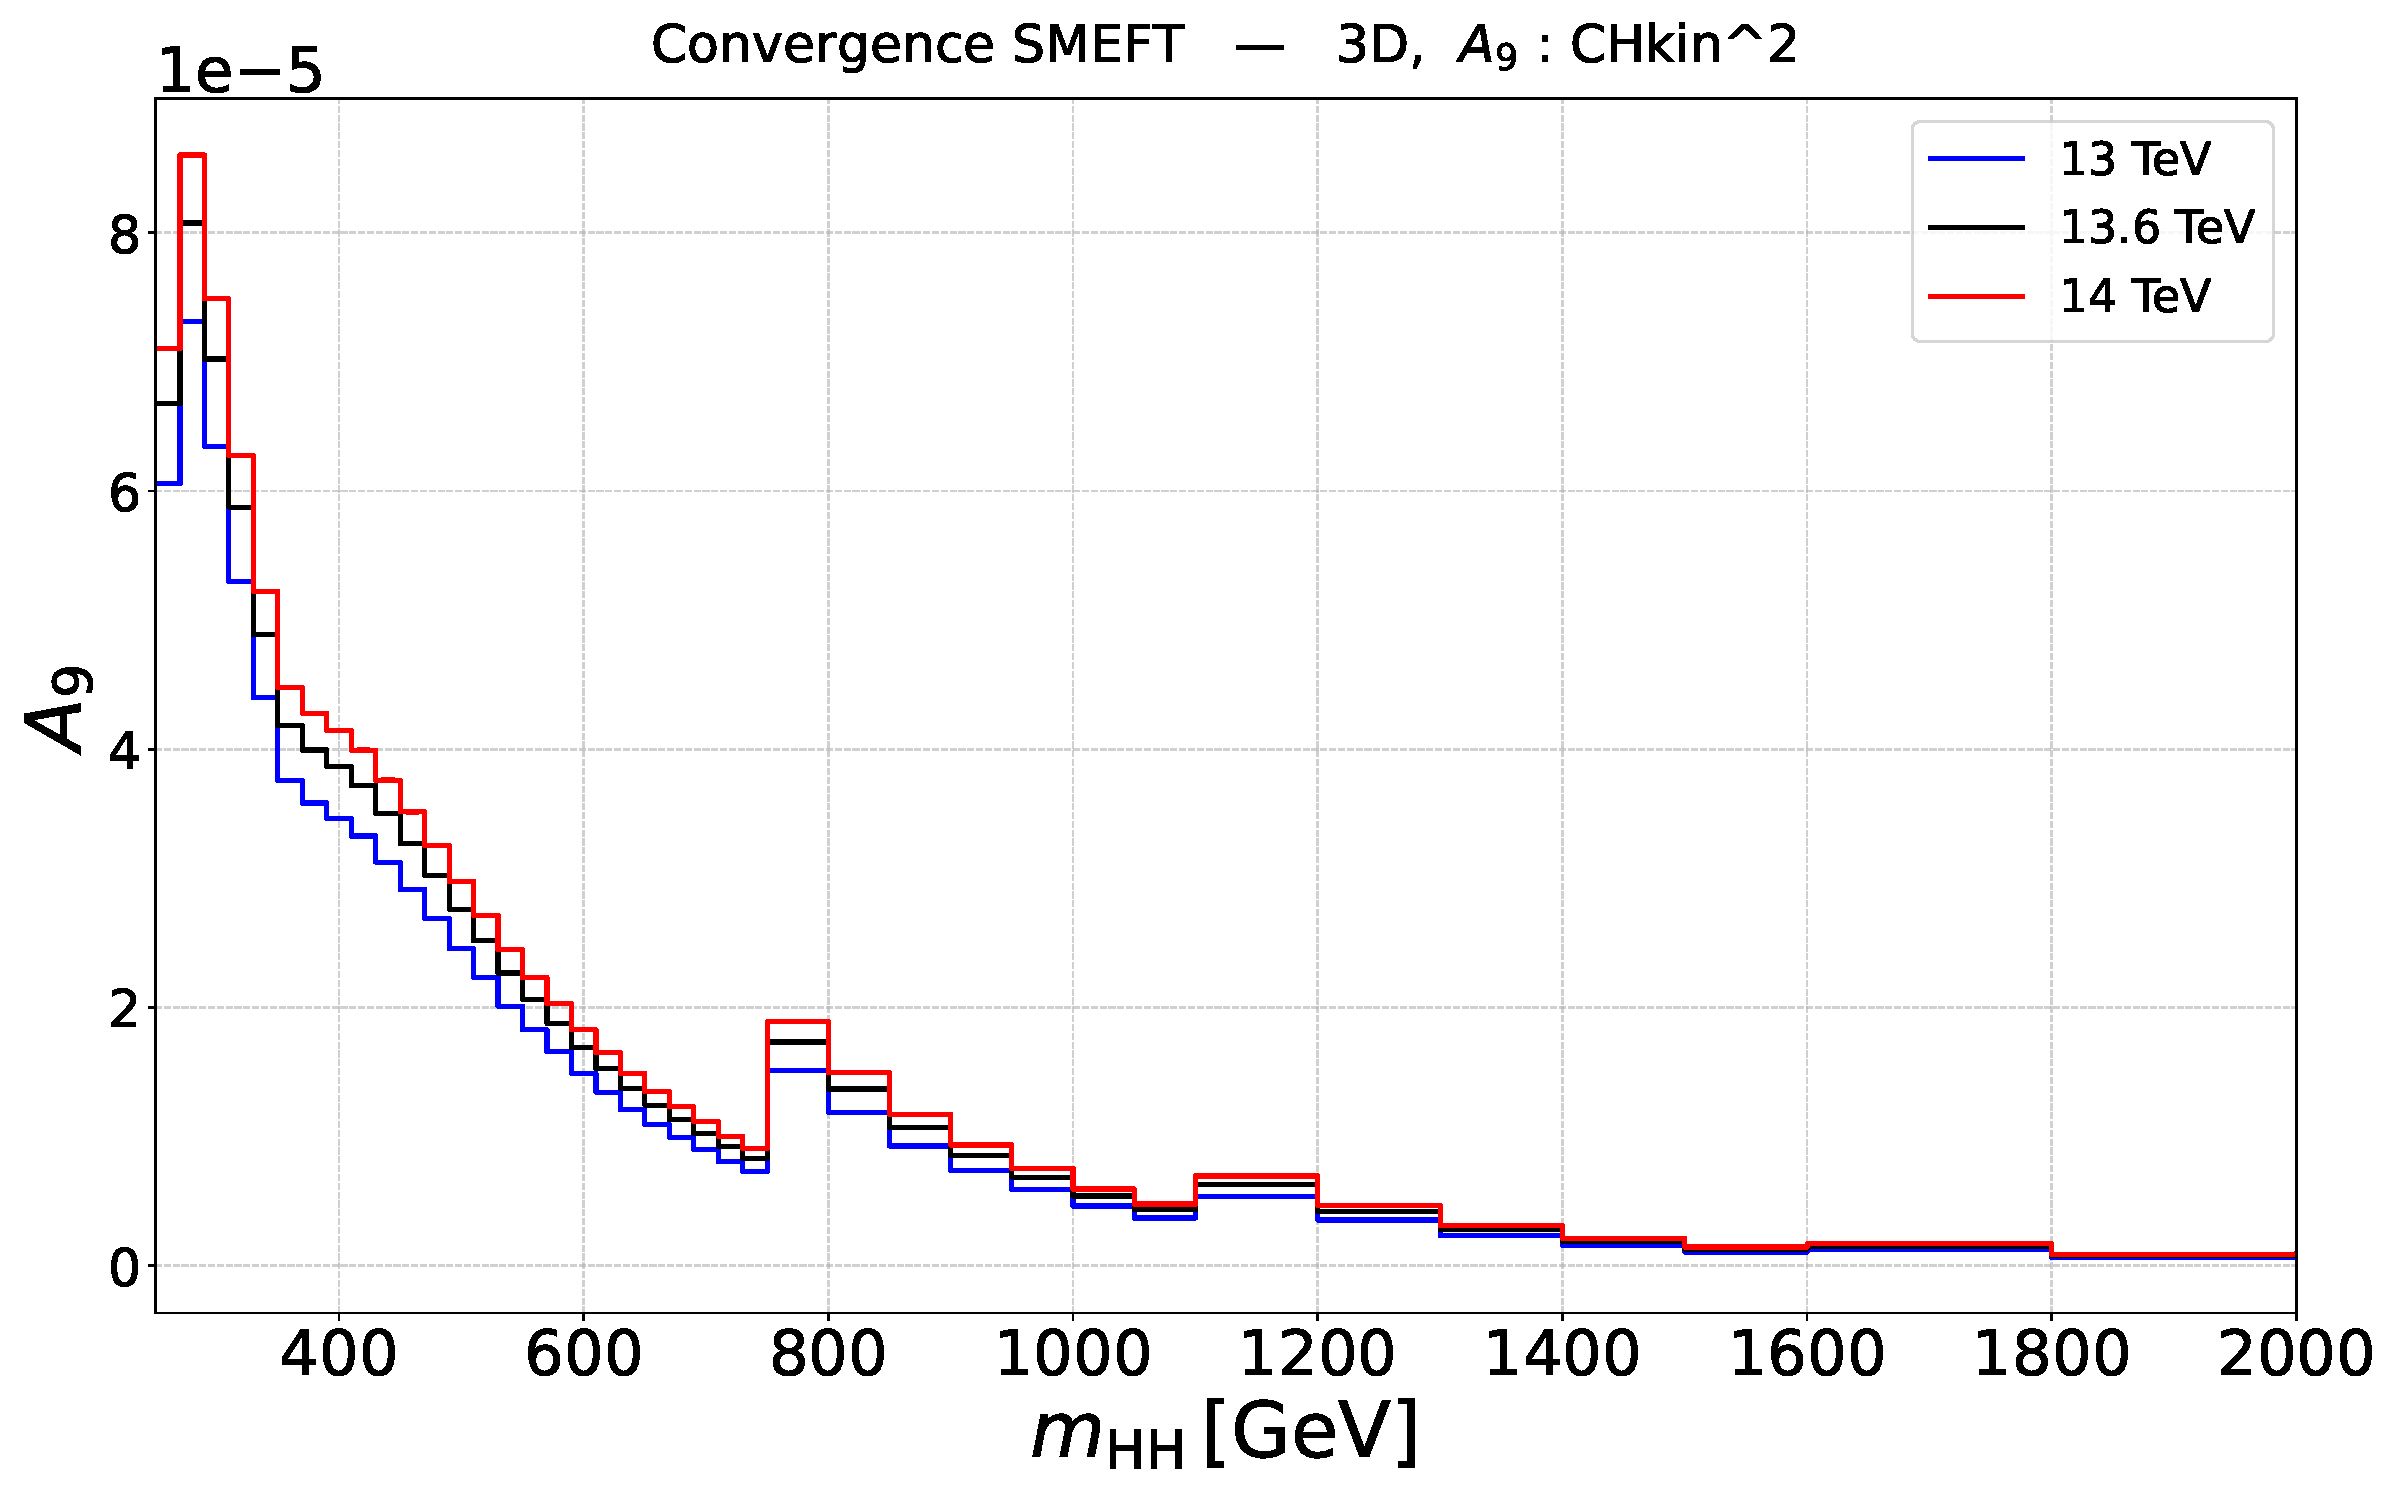
\includegraphics[width=\linew%idth]{plots/plot_param9_250_2000_3d_energy_13_13p6_14TeV.pdf}
  %\end{minipage}
  %\vspace{0.5em}
  %\begin{minipage}[b]{0.495\linewidth}
   % \centering
    %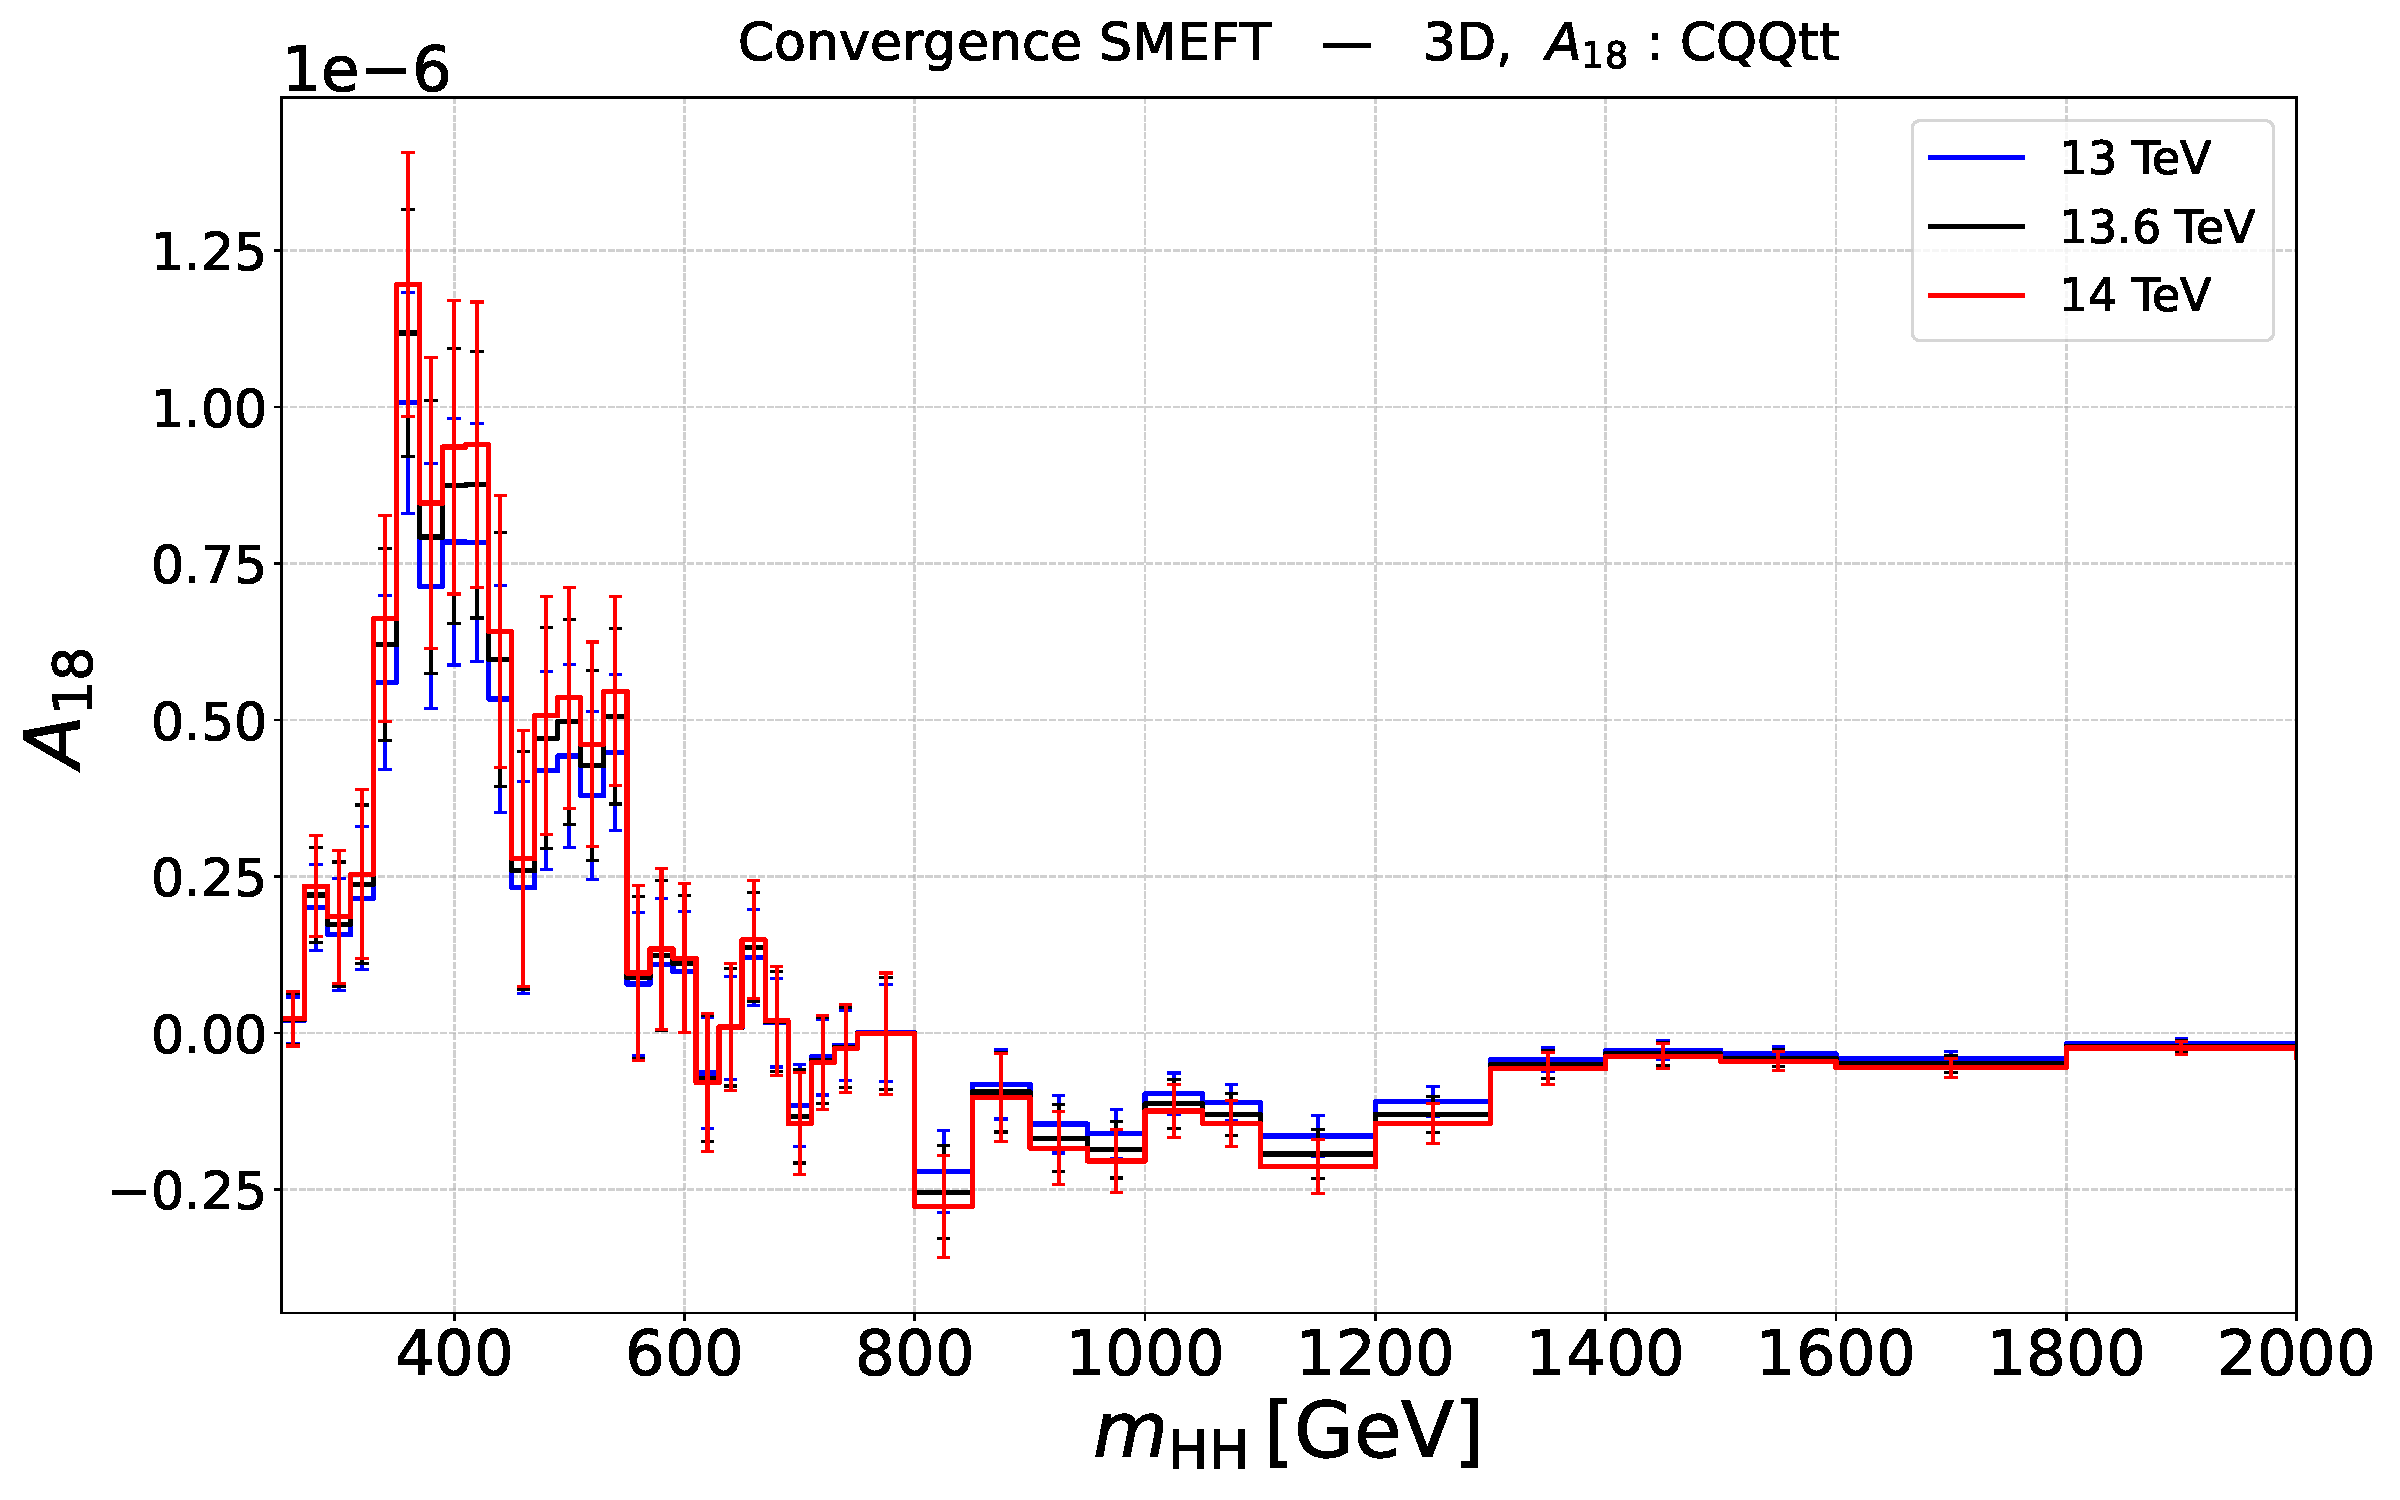
\includegraphics[width=\linew%idth]{plots/plot_param18_250_2000_3d_energy_13_13p6_14TeV.pdf}
  %\end{minipage}
  %\hfill
  %\begin{minipage}[b]{0.495\linewidth}
  %  \centering
    %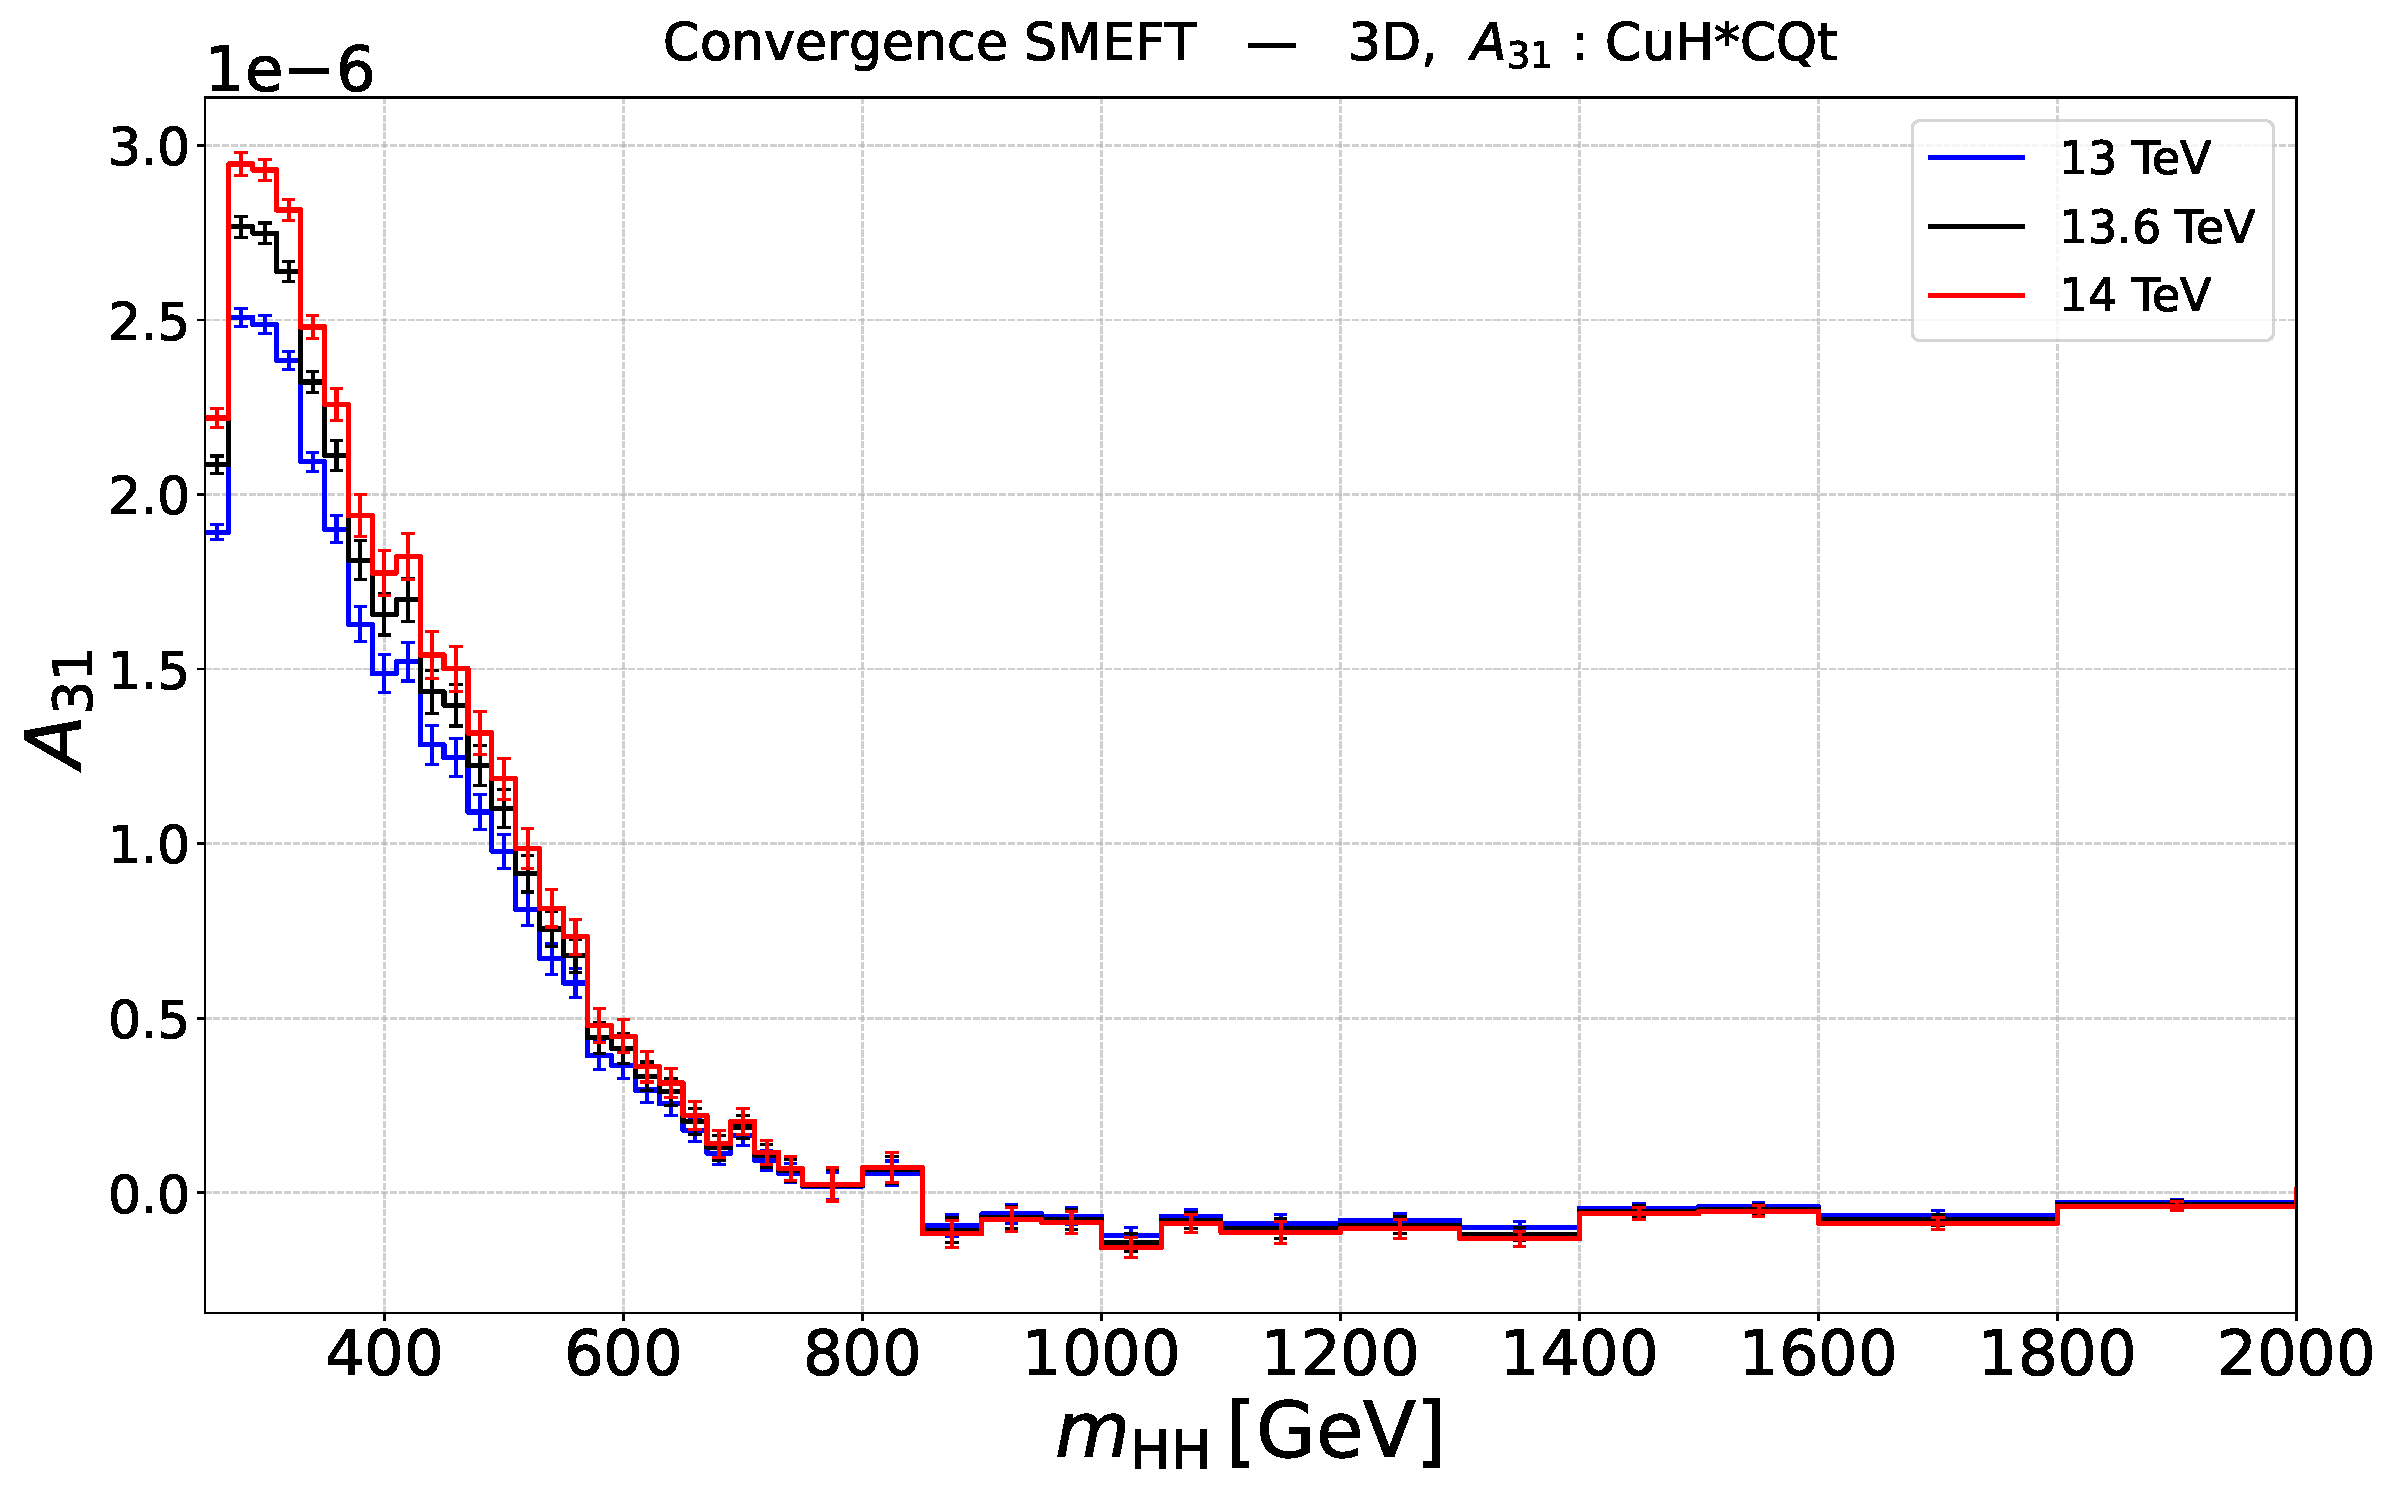
\includegraphics[width=\linewidth]{plots/plot_param31_250_2000_3d_energy_13_13p6_14TeV.pdf}
  %\end{minipage}
  %\caption{Convergence of the 3D $A$-coefficients projected into $m_{\text{HH}}$, for the three COM energies. The upper panel shows coefficients arising from leading-operator terms, while the lower panel shows coefficients arising from subleading and leading$\times$subleading terms.}
  %\label{fig:convergence_allCOM}
%\end{figure}
\section{Exchanging between authors}
\label{sec:appendix_exchange}

This appendix records the cross-checks made between parameterizations derived
independently by different authors, and the numbers exchanged for them.

\subsection{Cross sections at the Warsaw top-dipole basis points}
\label{sec:appendix_exchange_topdipole}

The five-coefficient ``Warsaw top-dipole'' parameterization of Ref.~\cite{ELR_topdipole} and the
nine-coefficient parameterization of this report describe the same process in overlapping regions of
the same parameter space, from separate simulated samples and separate fits. A direct comparison of
the total cross section at the twenty basis points of the former is therefore a check of both, and
it is reported in Table~\ref{tab:appendix_topdipole_xsec}.

The comparison is between two \emph{parameterizations}, not between a parameterization and a
generated cross section: the quoted values of the five-coefficient model are themselves the output
of its reweighting formula. The offset at the SM point, where the nine-coefficient formula gives
$31.01$~fb against $30.81$~fb, is the baseline difference between the two productions rather than an
error in either.

Two things bear on the remaining differences. First, thirteen of the twenty
points lie outside the hyper-rectangle in which the samples of this report were generated
(Table~\ref{tab:SMEFTcouplings}): $c_{\PH\mathrm{kin}}$ reaches $\pm 50$ against the $\pm 8$
generated here, and $c_{\PQt\PH}$ reaches $\pm 49$ against $[-10, 7]$. At those points the
nine-coefficient formula is being extrapolated, in one coordinate by a factor of five to seven.
Second, the differences are not spread evenly over the points but track $c_{\PQt\PH}$: the six
points with $c_{\PQt\PH} \neq 0$ differ by $2.2\%$ in median and by at most $3.4\%$, while the
fourteen points with $c_{\PQt\PH} = 0$ agree to $0.22\%$ in median and $0.65\%$ at worst. Since
$c_{\PQt\PH}$ is also the coordinate that is extrapolated furthest, the two observations are
consistent with a single explanation, and separating an extrapolation effect from a genuine
difference between the two fits would require points with $c_{\PQt\PH} \neq 0$ inside the generated
range.

Over all twenty points the median relative difference is $+0.07\%$, the median of its absolute value
$0.35\%$, and the largest $3.40\%$.

\begin{table}[ht]
\centering
\small
\begin{tabular}{ccccc|ccc}
\hline
$c_{\PH}$ & $c_{\PH\mathrm{kin}}$ & $c_{\PQt\PH}$ & $c_{\PH G}$ & $c_{\PQt G}$ &
$\sigma_{\text{5D}}$ [fb] & $\sigma_{\text{9D}}$ [fb] & difference [\%] \\
\hline
$0$ & $0$ & $0$ & $0$ & $0$ & $30.81$ & $31.01$ & $+0.64$ \\
$0$ & $8.174$ & $0$ & $0$ & $0$ & $33.60$ & $33.68$ & $+0.23$ \\
$0$ & $-10.02$ & $0$ & $0$ & $0$ & $188.56$ & $188.19$ & $-0.20$ \\
$47.01$ & $0$ & $0$ & $0$ & $0$ & $5626.66$ & $5619.30$ & $-0.13$ \\
$-10.41$ & $0$ & $0$ & $0$ & $0$ & $144.58$ & $144.36$ & $-0.15$ \\
$0$ & $0$ & $-11.24$ & $0$ & $0$ & $78.82$ & $80.42$ & $+2.03$$^{\ast}$ \\
$0$ & $0$ & $-5.332$ & $0$ & $0$ & $19.77$ & $20.13$ & $+1.80$$^{\ast}$ \\
$0$ & $0$ & $0$ & $0.08801$ & $0$ & $222.12$ & $221.67$ & $-0.20$ \\
$0$ & $0$ & $0$ & $-0.0934$ & $0$ & $424.25$ & $423.75$ & $-0.12$ \\
$21.48$ & $31.95$ & $0$ & $0$ & $0$ & $316.89$ & $316.66$ & $-0.07$ \\
$0$ & $-46.72$ & $-33.62$ & $0$ & $0$ & $348.30$ & $339.59$ & $-2.50$$^{\ast}$ \\
$0$ & $37.37$ & $0$ & $-0.08705$ & $0$ & $408.20$ & $405.57$ & $-0.65$ \\
$0$ & $49.99$ & $49.34$ & $0$ & $0$ & $364.06$ & $372.38$ & $+2.29$$^{\ast}$ \\
$0$ & $0$ & $42.59$ & $0.04191$ & $0$ & $1824.62$ & $1854.80$ & $+1.65$$^{\ast}$ \\
$0$ & $2.355$ & $0$ & $-0.03882$ & $0$ & $81.85$ & $82.02$ & $+0.21$ \\
$0$ & $27.12$ & $0$ & $0$ & $-0.957$ & $390.54$ & $389.35$ & $-0.31$ \\
$0$ & $-2.418$ & $0$ & $0$ & $0.2247$ & $44.87$ & $45.05$ & $+0.40$ \\
$0$ & $0$ & $-11.06$ & $0$ & $-0.7811$ & $54.49$ & $56.34$ & $+3.40$$^{\ast}$ \\
$0$ & $0$ & $0$ & $0.09657$ & $-1$ & $203.18$ & $202.36$ & $-0.40$ \\
$0$ & $0$ & $0$ & $0$ & $-0.8087$ & $49.25$ & $49.37$ & $+0.24$ \\
\hline
\end{tabular}
\caption{Total \ggHH cross section at $13.6$~TeV at the twenty basis points of the
five-coefficient Warsaw top-dipole parameterization, as given by that parameterization
($\sigma_{\text{5D}}$) and as computed from the nine-coefficient parameterization of this report
($\sigma_{\text{9D}}$), with their relative difference. The two describe the same process from
separate samples and separate fits. Points marked $^{\ast}$ have $c_{\PQt\PH} \neq 0$; these are
also the points extrapolated furthest beyond the range in which the samples of this report were
generated. The remaining four Wilson coefficients of the nine-coefficient parameterization are zero
at every point.}
\label{tab:appendix_topdipole_xsec}
\end{table}


\clearpage
\section{Additional uncertainty scans}
\label{sec:appendix_performance}

The seven one-dimensional scans not shown in Sec.~\ref{sec:uncertainties}, in the
same format: the predicted \ggHH cross section along one Wilson coefficient
with the other eight at zero, the interpolation uncertainty of
Eq.~\eqref{eq:sigmainterp}, and the same uncertainty as a fraction of the yield
in the lower panel. The dotted line is the SM.

\begin{figure}[htbp]
    \centering
    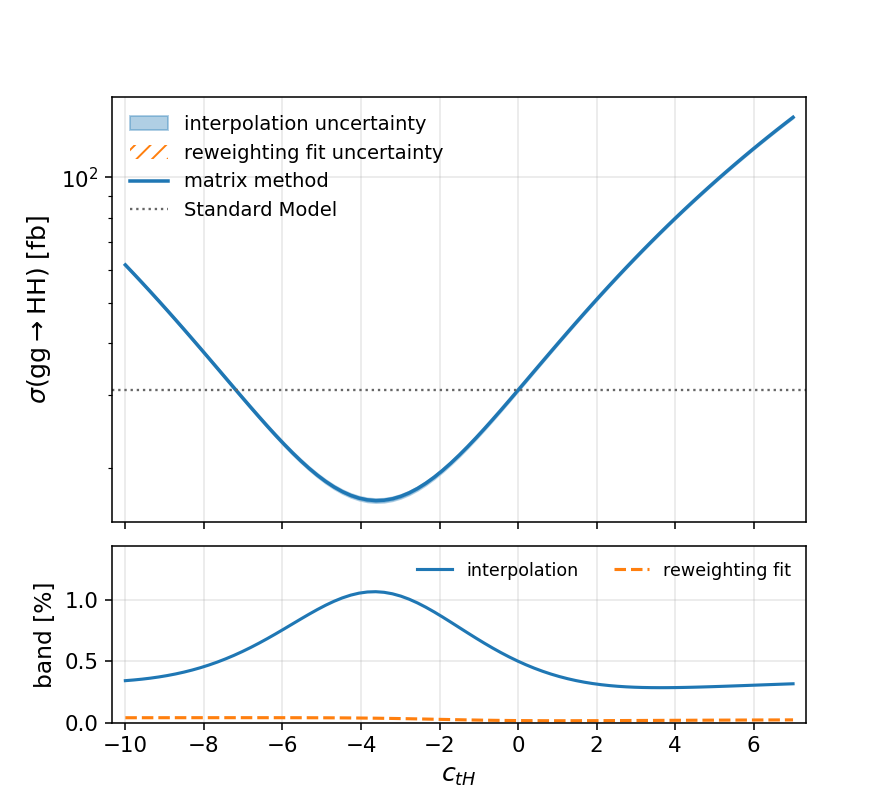
\includegraphics[width=0.40\textwidth]{figures/basis_optimization/unc_yield_ctH.png}
    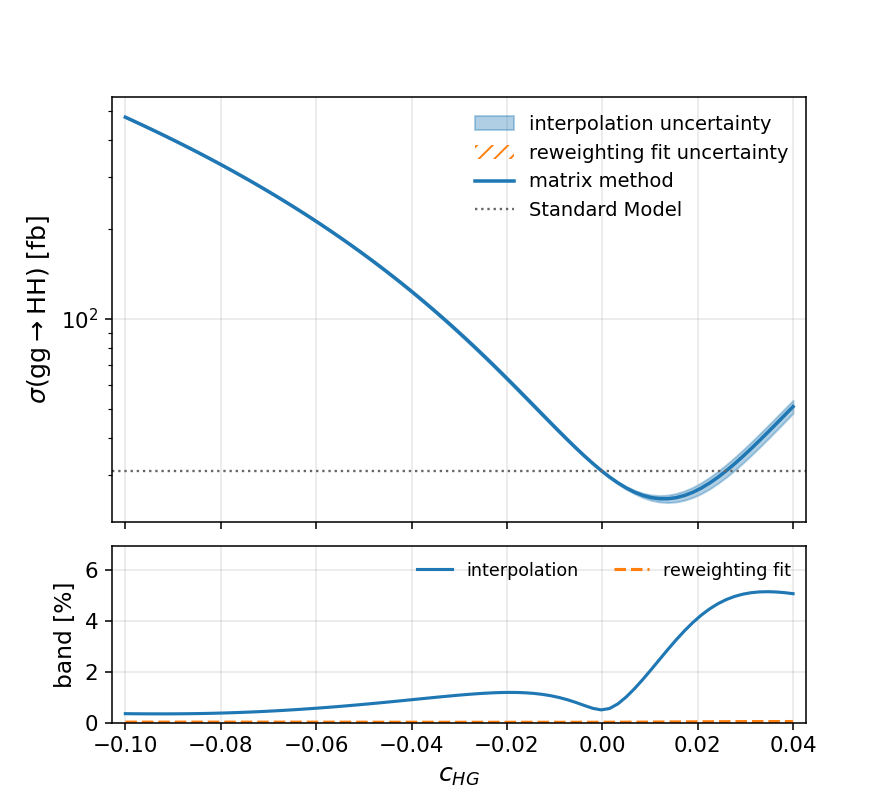
\includegraphics[width=0.40\textwidth]{figures/basis_optimization/unc_yield_cHG.png}\\
    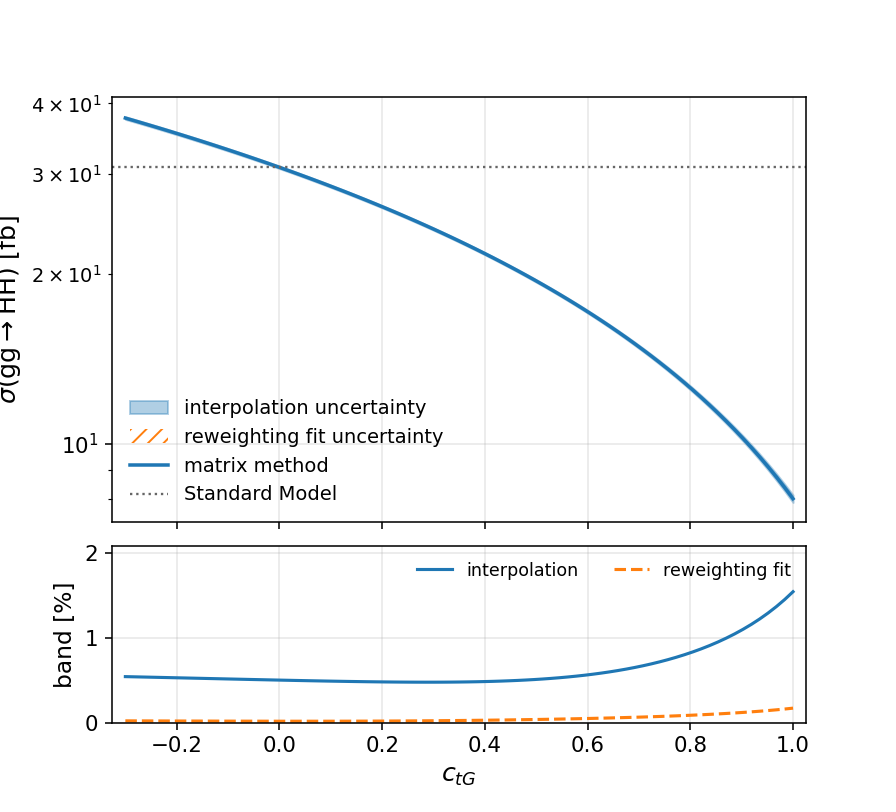
\includegraphics[width=0.40\textwidth]{figures/basis_optimization/unc_yield_ctG.png}
    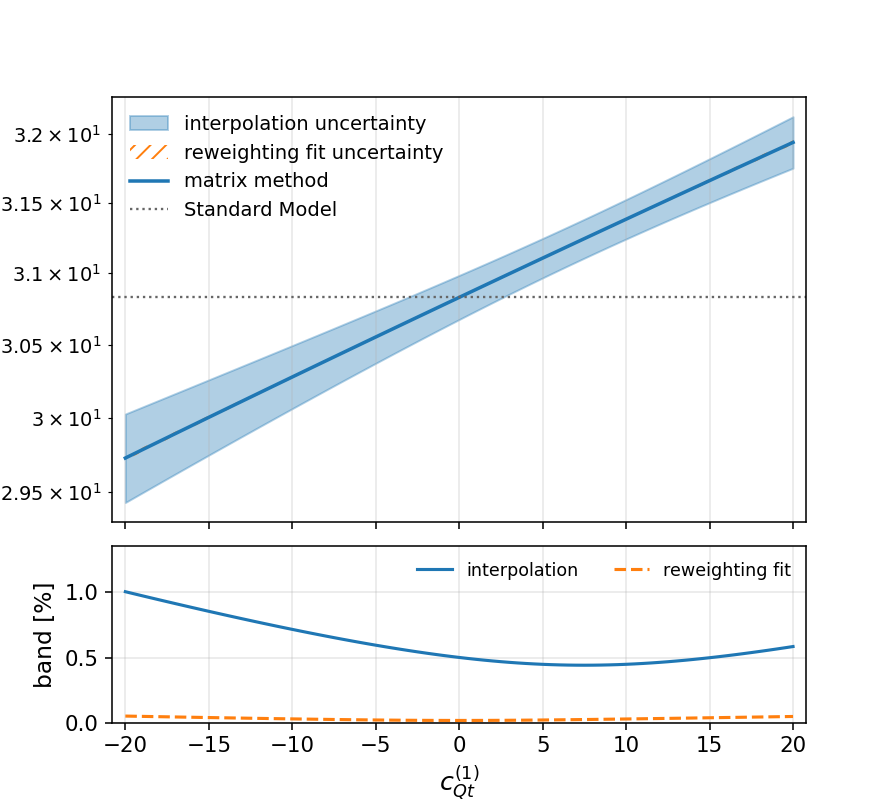
\includegraphics[width=0.40\textwidth]{figures/basis_optimization/unc_yield_cQt1.png}
    \caption{Scans along $c_{\PQt\PH}$, $c_{\PH G}$, $c_{\PQt G}$ and
    $c_{Q\PQt}^{(1)}$.}
    \label{fig:unc_yield_extra1}
\end{figure}

\begin{figure}[htbp]
    \centering
    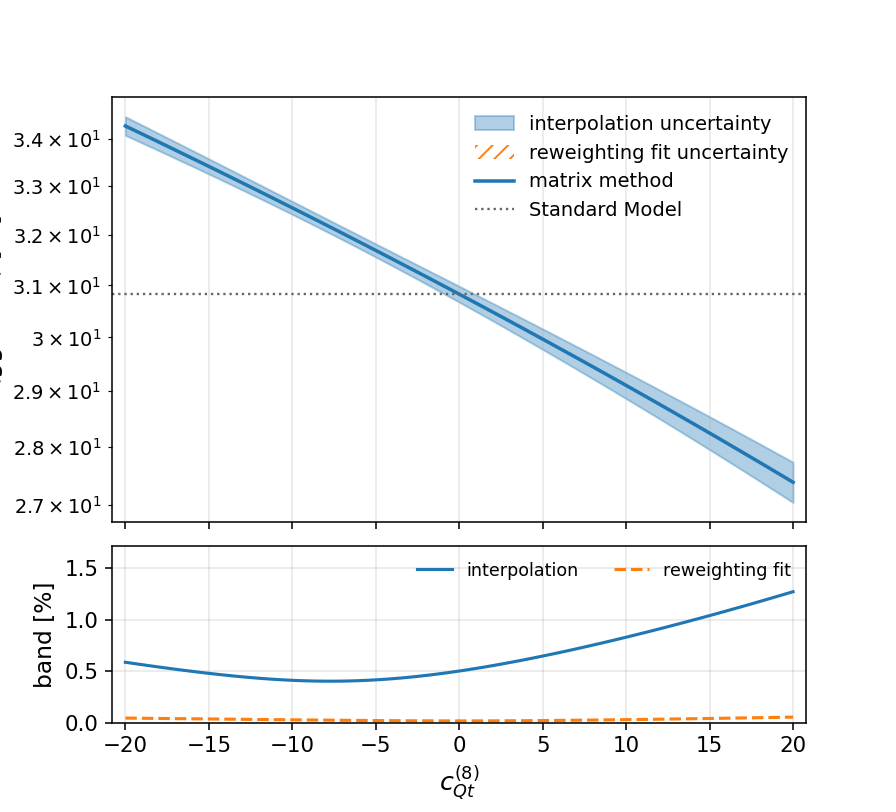
\includegraphics[width=0.40\textwidth]{figures/basis_optimization/unc_yield_cQt8.png}
    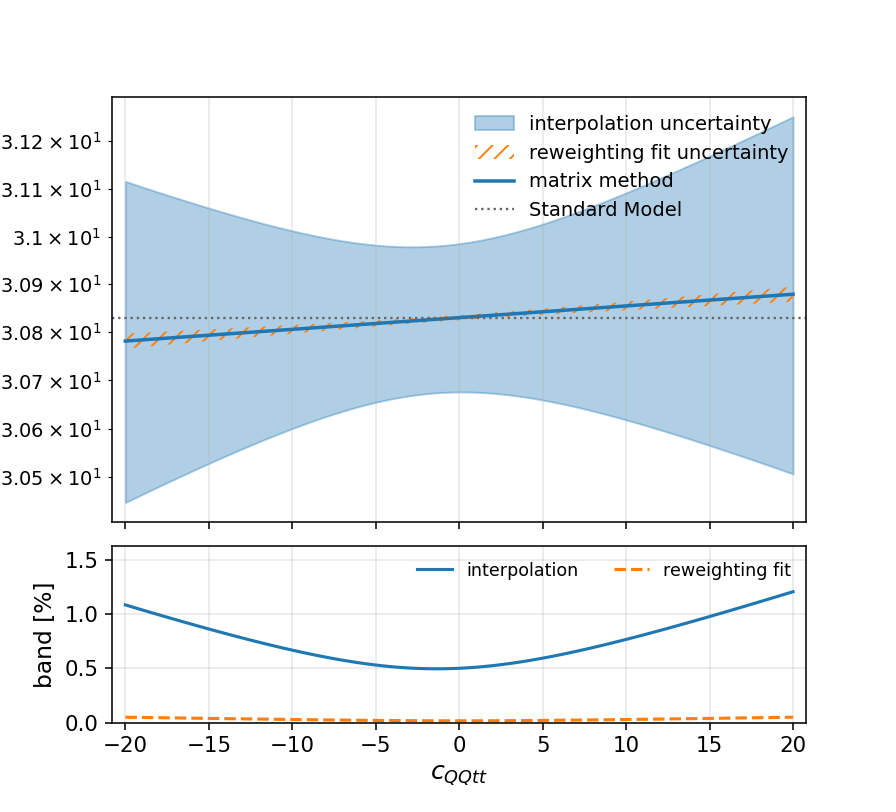
\includegraphics[width=0.40\textwidth]{figures/basis_optimization/unc_yield_cQQtt.png}\\
    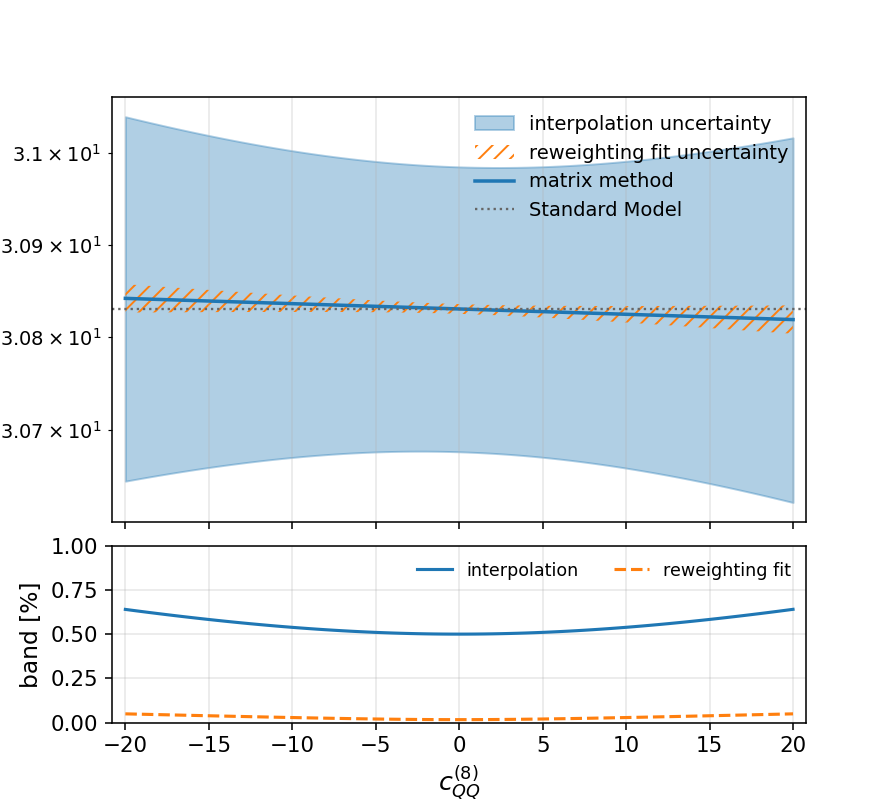
\includegraphics[width=0.40\textwidth]{figures/basis_optimization/unc_yield_cQQ8.png}
    \caption{Scans along $c_{Q\PQt}^{(8)}$, $c_{QQ\PQt\PQt}$ and $c_{QQ}^{(8)}$.}
    \label{fig:unc_yield_extra2}
\end{figure}

\begin{table}[htbp]
\centering
\begin{tabular}{l|cc|cc}
\hline
 & \multicolumn{2}{c|}{band, fraction of the yield} &
   \multicolumn{2}{c}{scanned range} \\
coefficient & smallest & largest & from & to \\
\hline
$c_{\PH}$               & $0.2\%$ & $5.8\%$ & $-50$   & $50$   \\
$c_{\PH\mathrm{kin}}$   & $0.3\%$ & $0.7\%$ & $-8$    & $8$    \\
$c_{\PQt\PH}$           & $0.3\%$ & $1.1\%$ & $-10$   & $7$    \\
$c_{\PH G}$             & $0.3\%$ & $5.1\%$ & $-0.1$  & $0.04$ \\
$c_{\PQt G}$            & $0.5\%$ & $1.5\%$ & $-0.3$  & $1$    \\
$c_{Q\PQt}^{(1)}$       & $0.4\%$ & $1.0\%$ & $-20$   & $20$   \\
$c_{Q\PQt}^{(8)}$       & $0.4\%$ & $1.3\%$ & $-20$   & $20$   \\
$c_{QQ\PQt\PQt}$        & $0.5\%$ & $1.2\%$ & $-20$   & $20$   \\
$c_{QQ}^{(8)}$          & $0.5\%$ & $0.6\%$ & $-20$   & $20$   \\
\hline
\end{tabular}
\caption{Range of the interpolation uncertainty as a fraction of the predicted
yield, over each one-dimensional scan. Every scan passes through $0.50\%$ at the
SM.}
\label{tab:unc_bands}
\end{table}

\begin{table}[htbp]
\centering
\begin{tabular}{l|cc}
\hline
plane & median $|\Delta|/|\Delta|_\mathrm{stat}$ & bins with $|$pull$|<1$ \\
\hline
$c_{\PH}$--$c_{\PQt\PH}$                 & $0.74$ & $0.72$ \\
$c_{\PH}$--$c_{\PH G}$                   & $0.71$ & $0.74$ \\
$c_{\PH}$--$c_{\PQt G}$                  & $0.71$ & $0.67$ \\
$c_{\PH\mathrm{kin}}$--$c_{\PQt\PH}$     & $0.88$ & $0.71$ \\
$c_{Q\PQt}^{(1)}$--$c_{QQ}^{(8)}$        & $0.65$ & $0.76$ \\
\hline
\end{tabular}
\caption{Size of the interpolation uncertainty against the residual actually
observed, per plane of the generated grid. The first column is the median over
the plane of the ratio defined in Sec.~\ref{sec:uncertainties}, the second the
fraction of bins whose pull is within one standard deviation; a standard normal
gives $0.683$.}
\label{tab:unc_calibration}
\end{table}

\subsection{The modelling uncertainty per selection}
\label{sec:appendix_unc_per_selection}
\label{sec:appendix_unc_realistic}

The two terms that make up $\sigma_\mathrm{mod}$ are given separately in
Tab.~\ref{tab:unc_components}. Which of them dominates is not a property of the
method but of the selection and the coefficient: $\sigma_\mathrm{ELR}$ is the
larger in the resolved selection for every coefficient, and in the merged one
for four of the six, while for $c_{\PH G}$ in the merged selection the ordering
inverts, that being where the merged templates are thinnest. The composition of one
entry therefore does not carry to the others.

\begin{table}[htbp]
\centering
\begin{tabular}{l|ccc|ccc}
\hline
 & \multicolumn{3}{c|}{$4\PQb$ resolved} & \multicolumn{3}{c}{$4\PQb$ fully merged} \\
coefficient & $\sigma_\mathrm{MM}$ & $\sigma_\mathrm{ELR}$ & $\sigma_\mathrm{mod}$ & $\sigma_\mathrm{MM}$ & $\sigma_\mathrm{ELR}$ & $\sigma_\mathrm{mod}$ \\
\hline
$c_\PH$                & $0.20\%$ & $0.49\%$ & $0.53\%$ & $1.48\%$ & $3.39\%$ & $3.77\%$ \\
$c_{\PH\mathrm{kin}}$  & $0.17\%$ & $1.14\%$ & $1.16\%$ & $1.20\%$ & $1.73\%$ & $2.01\%$ \\
$c_{\PQt\PH}$          & $0.22\%$ & $0.96\%$ & $0.98\%$ & $1.17\%$ & $1.47\%$ & $1.86\%$ \\
$c_{\PH G}$            & $0.28\%$ & $0.97\%$ & $1.02\%$ & $2.76\%$ & $0.62\%$ & $2.85\%$ \\
$c_{\PQt G}$           & $0.14\%$ & $1.50\%$ & $1.50\%$ & $0.99\%$ & $3.03\%$ & $3.17\%$ \\
$c_{Q\PQt}^{(1)}$      & $0.20\%$ & $0.63\%$ & $0.65\%$ & $1.94\%$ & $1.40\%$ & $2.33\%$ \\
\hline
\end{tabular}
\caption{The two terms of the modelling uncertainty of
Fig.~\ref{fig:unc_realistic_cH}, as a fraction of the predicted yield, at the
median of each one-dimensional scan with the other eight coefficients at zero.
$\sigma_\mathrm{MM}$ is the Monte Carlo statistical error of the basis
templates propagated through the morphing weights, $\sigma_\mathrm{ELR}$ the
uncertainty of the reweighting coefficients the templates were made with, and
$\sigma_\mathrm{mod}^2=\sigma_\mathrm{MM}^2+\sigma_\mathrm{ELR}^2$ the quantity
drawn in the lower panel of those figures. The weights are the same in both
pairs of columns; the template errors are each selection's own.}
\label{tab:unc_components}
\end{table}

The six scans of Sec.~\ref{sec:validation_realistic_band} follow, in a common format:
the predicted yield after the resolved and the fully merged selection along one Wilson
coefficient, with the modelling uncertainty $\sigma_{\text{mod}}$ of
Eq.~\eqref{eq:sigmainterp} combined with the reweighting term as a band, and the band size as a fraction of the yield in the
lower pad.

\begin{figure}[htbp]
    \centering
    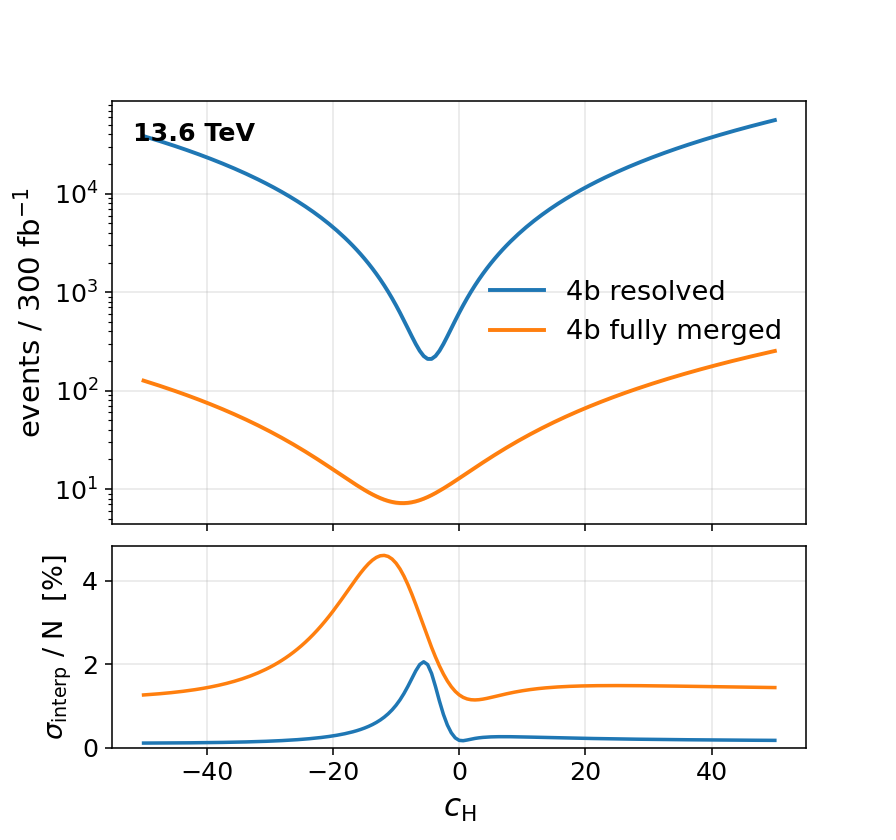
\includegraphics[width=0.52\textwidth]
        {figures/basis_optimization/realistic_unc_cH.png}
    \caption{Predicted yield after the resolved and the fully merged
    $\HH\to\bbbar\bbbar$ selections along $c_{\PH}$, with the modelling uncertainty as a
    band; lower pad, the band size as a fraction of the yield.}
    \label{fig:unc_realistic_cH}
\end{figure}

\begin{figure}[htbp]
    \centering
    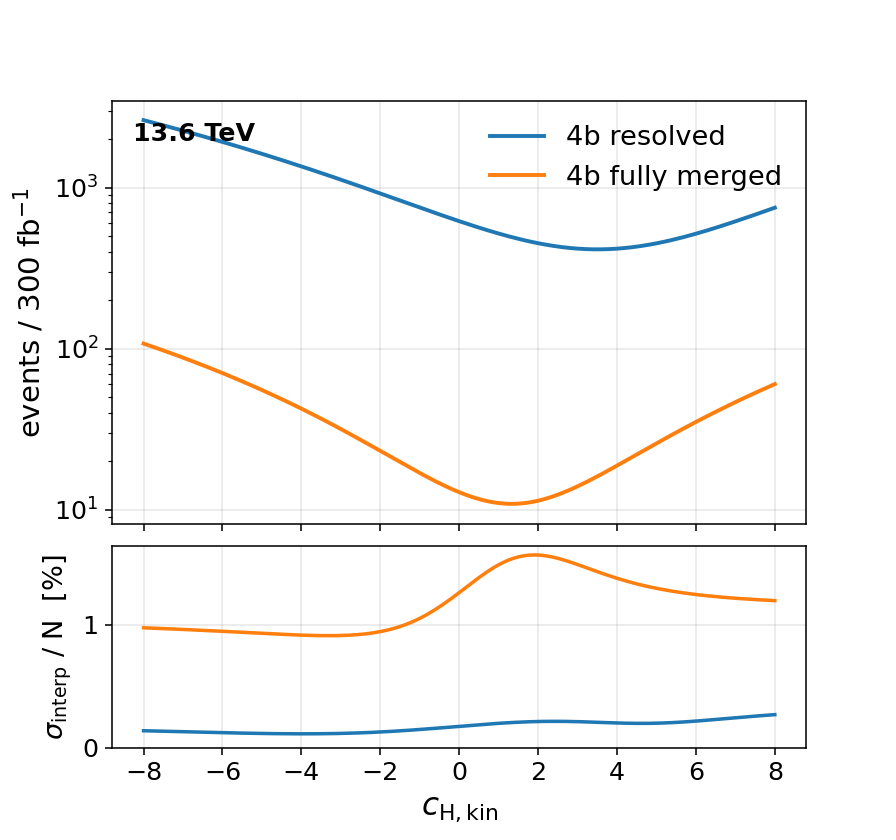
\includegraphics[width=0.52\textwidth]
        {figures/basis_optimization/realistic_unc_cHkin.png}
    \caption{The same quantities as in Fig.~\ref{fig:unc_realistic_cH}, along
    $c_{\PH\mathrm{kin}}$.}
    \label{fig:unc_realistic_cHkin}
\end{figure}

\begin{figure}[htbp]
    \centering
    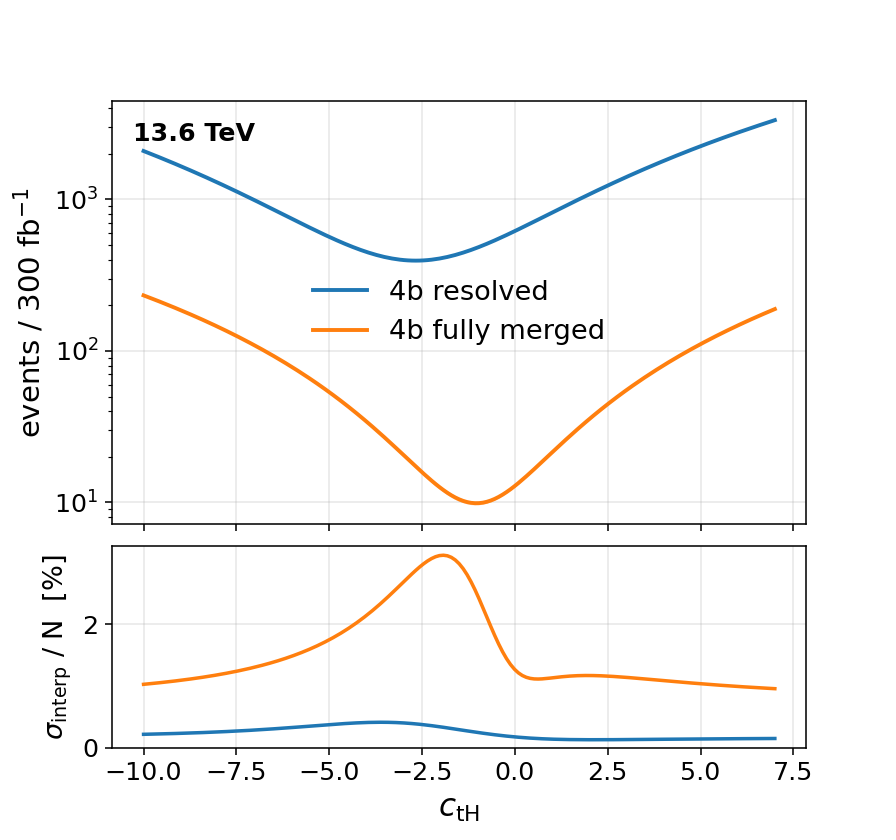
\includegraphics[width=0.52\textwidth]
        {figures/basis_optimization/realistic_unc_ctH.png}
    \caption{The same quantities as in Fig.~\ref{fig:unc_realistic_cH}, along
    $c_{\PQt\PH}$.}
    \label{fig:unc_realistic_ctH}
\end{figure}

\begin{figure}[htbp]
    \centering
    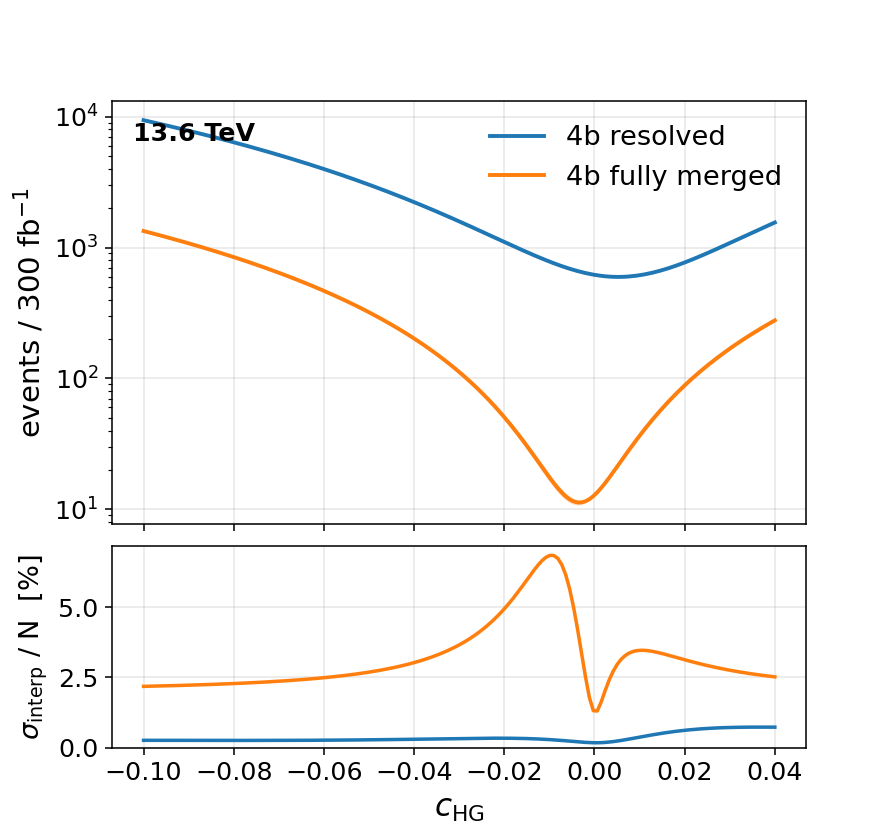
\includegraphics[width=0.52\textwidth]
        {figures/basis_optimization/realistic_unc_cHG.png}
    \caption{The same quantities as in Fig.~\ref{fig:unc_realistic_cH}, along
    $c_{\PH G}$.}
    \label{fig:unc_realistic_cHG}
\end{figure}

\begin{figure}[htbp]
    \centering
    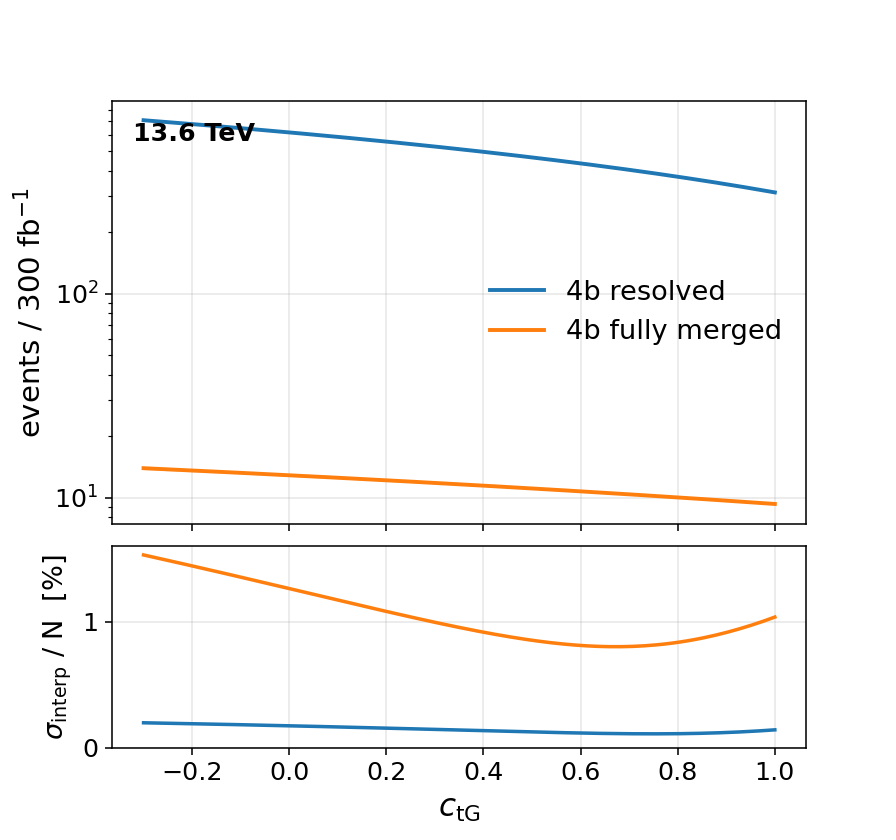
\includegraphics[width=0.52\textwidth]
        {figures/basis_optimization/realistic_unc_ctG.png}
    \caption{The same quantities as in Fig.~\ref{fig:unc_realistic_cH}, along
    $c_{\PQt G}$.}
    \label{fig:unc_realistic_ctG}
\end{figure}

\begin{figure}[htbp]
    \centering
    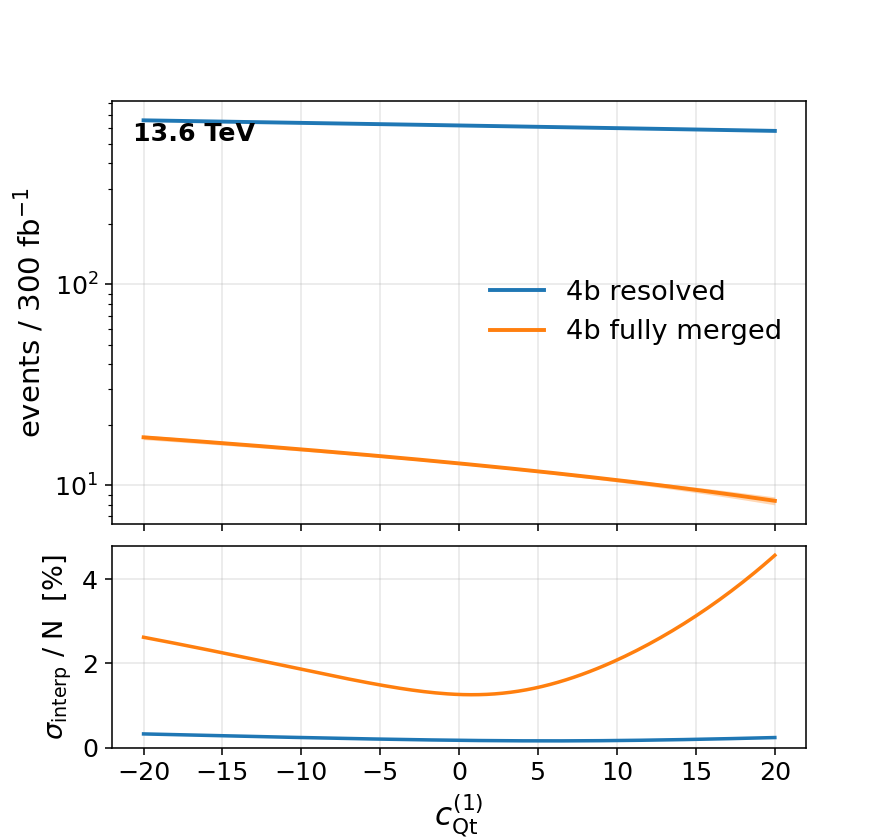
\includegraphics[width=0.52\textwidth]
        {figures/basis_optimization/realistic_unc_cQt1.png}
    \caption{The same quantities as in Fig.~\ref{fig:unc_realistic_cH}, along
    $c_{Q\PQt}^{(1)}$.}
    \label{fig:unc_realistic_cQt1}
\end{figure}

For reference, the same band evaluated on the inclusive cross section, with no
selection applied, is shown below. It is one band rather than two because there
is one set of $\sigma_i$; this is the figure that
Sec.~\ref{sec:validation_realistic_band} replaces with a measurement.

\begin{figure}[htbp]
    \centering
    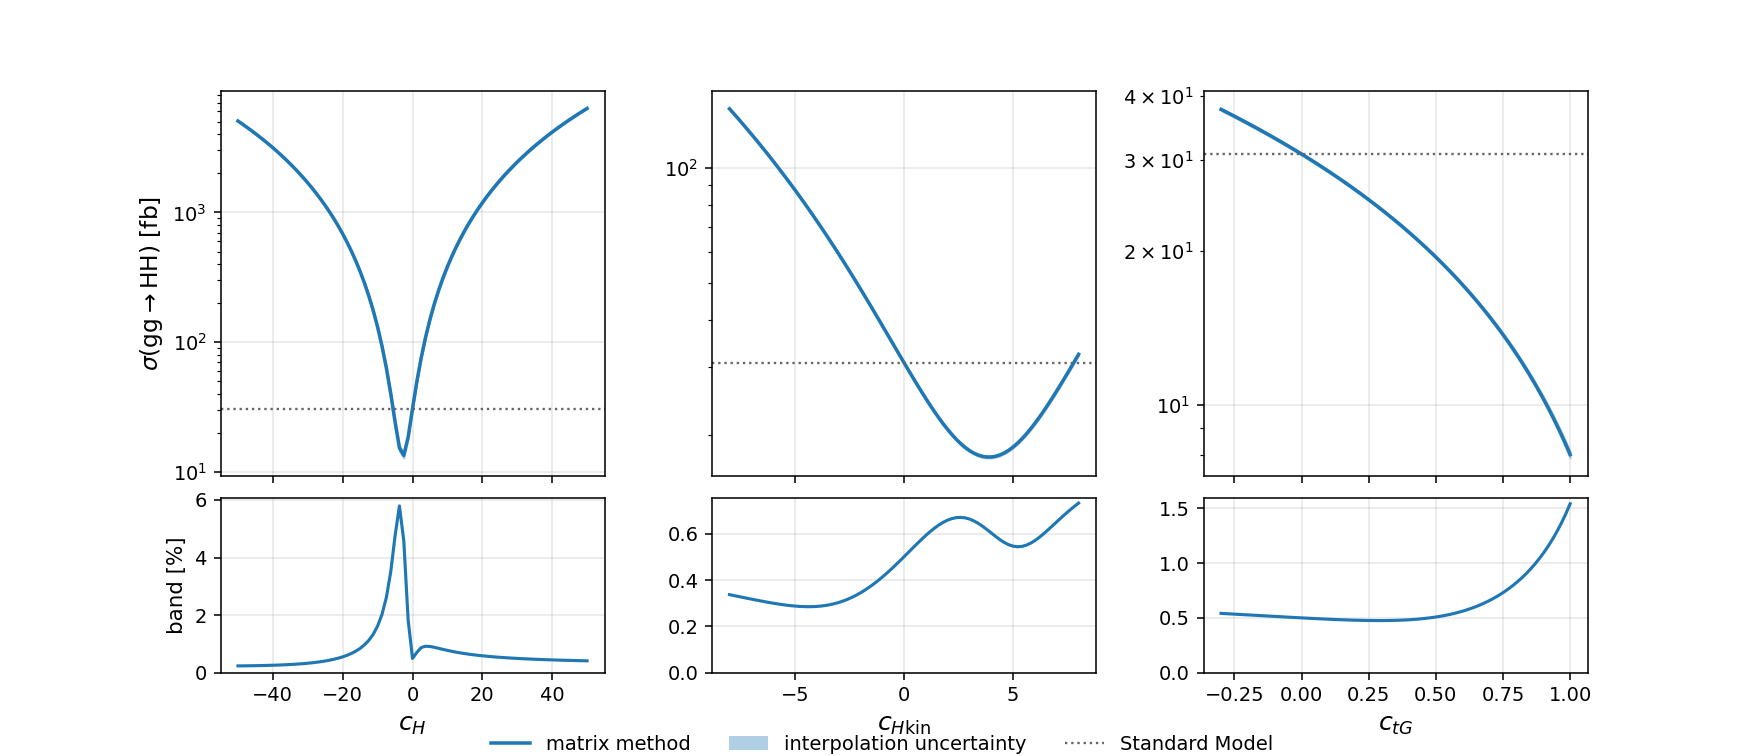
\includegraphics[width=\textwidth]
        {figures/basis_optimization/unc_yield_row.png}
    \caption{Predicted \ggHH cross section along $c_\PH$, $c_{\PH\mathrm{kin}}$
    and $c_{\PQt G}$, in each case with the other eight coefficients at zero,
    with the interpolation uncertainty of Eq.~\eqref{eq:sigmainterp}. The dotted
    line is the SM. The lower panels repeat the uncertainty as a
    fraction of the yield. Note the different vertical scales.}
    \label{fig:unc_yield}
\end{figure}

\subsection{\textcolor{red}{[AUTHORS ONLY]} The same uncertainty in the HEFT basis}
\label{sec:appendix_heft_unc}

\textcolor{red}{This subsection is for the authors and is not intended for the
published version. It is here to record that the prescription is not specific to the
SMEFT parameterization, and to give the numbers for the HEFT basis before deciding
whether any of it belongs in the report.}

Nothing in Eq.~\eqref{eq:sigmainterp} refers to SMEFT. It needs a basis, the
parameterization the weights are solved from, and the statistical errors of the
templates. Replacing the forty SMEFT monomials by the twenty-three of the
$\kappa$-framework HEFT parameterization in $\kappa_\lambda$, $\kappa_\PQt$, $c_2$,
$c_g$ and $c_{2g}$, and applying the same weights to the same two $4\PQb$ selections,
gives Table~\ref{tab:unc_heft}. The basis is the published twenty-three-point HEFT set,
square and of condition number $1.0\times10^{4}$, against $1.9\times10^{6}$ for the
forty-point SMEFT one.

The templates and their covariance are recomputed here from the input trees of the two
$4\PQb$ selections, one pass per input sample carrying every basis point's weight, so
the band can be given in both forms: the exact one, $\sqrt{w^{T}Sw}$ with the full
covariance of Eq.~\eqref{eq:sigmaMMcov}, and the independent one of
Eq.~\eqref{eq:sigmainterp}. The merged selection costs a factor five to eight over the
resolved one, as in the SMEFT case. The two forms differ most along $c_{2g}$, the
direction the twenty-three points constrain least: there the independent form gives
$3.54\%$ in the median and $9.49\%$ at its largest in the merged selection, against
$1.90\%$ and $2.04\%$ exactly, so the band that looked an order of magnitude worse than
the others is mostly the correlation between templates, counted twice. Bin by bin the
ratio of the two forms runs from $0.7$ to about $35$. At the SM the exact band is
$0.173\%$ of the resolved yield and $1.27\%$ of the merged one.

\textcolor{red}{Produced with \texttt{scripts/gghh\_smeft/mm\_covariance\_from\_trees.py}
and \texttt{mm\_covariance\_scans.py} of the toolkit, which reproduce the
\texttt{ELReweighter} templates in numpy: the integrated yields of the twenty-three basis
points agree with the delivered table to $0.1\%$ in the median (resolved).}

\textcolor{red}{The earlier version of this table, and the $18\%$ it quoted on $c_{2g}$,
came from the \texttt{err\_yield} column of that delivered table and should not be
quoted. That column is a factor $\simeq\sqrt{2}$ above the inverse-variance combination
of the same four inputs, uniformly over the twenty-three points and both regions
($0.70\pm0.03$). The card side reproduced the same ratio with the \texttt{ELReweighter}
itself, so the factor is in the table and not in the templates: the table was committed
from an external production and is written by no script of the package, and a doubled
\texttt{Sumw2} at filling or merging would produce exactly that flat factor. The numbers
above are built from the events and do not depend on it, and the SMEFT tables used
elsewhere in this report are written by \texttt{make\_datacards} from the same templates
the card uses, with errors equal to $\sqrt{S_{ii}}$ and no such factor --- consistently,
the resolved band at the SM is $0.17\%$ there as it is here.}

\begin{table}[htbp]
\centering
\begin{tabular}{l|cc|cc|cc|cc}
\hline
 & \multicolumn{4}{c|}{$4\PQb$ resolved} & \multicolumn{4}{c}{$4\PQb$ fully merged} \\
 & \multicolumn{2}{c|}{exact} & \multicolumn{2}{c|}{independent}
 & \multicolumn{2}{c|}{exact} & \multicolumn{2}{c}{independent} \\
coupling & median & largest & median & largest & median & largest & median & largest \\
\hline
$\kappa_\lambda$ & $0.20\%$ & $0.24\%$ & $0.21\%$ & $0.50\%$ & $1.37\%$ & $1.68\%$ & $1.48\%$ & $1.82\%$ \\
$\kappa_\PQt$    & $0.17\%$ & $0.19\%$ & $0.22\%$ & $0.38\%$ & $1.27\%$ & $1.27\%$ & $1.21\%$ & $1.23\%$ \\
$c_2$            & $0.22\%$ & $0.28\%$ & $0.23\%$ & $0.65\%$ & $1.36\%$ & $1.41\%$ & $1.49\%$ & $4.71\%$ \\
$c_g$            & $0.17\%$ & $0.18\%$ & $0.24\%$ & $0.34\%$ & $1.27\%$ & $1.27\%$ & $1.20\%$ & $2.54\%$ \\
$c_{2g}$         & $0.26\%$ & $0.43\%$ & $0.38\%$ & $0.50\%$ & $1.90\%$ & $2.04\%$ & $3.54\%$ & $9.49\%$ \\
\hline
\end{tabular}
\caption{\textcolor{red}{[AUTHORS ONLY]} Interpolation uncertainty as a fraction of the
predicted yield, median and largest over each one-dimensional scan, for the
twenty-three-point HEFT basis and the two $4\PQb$ selections of Ref.~\cite{CMS:2026znu}.
``Exact'' is $\sqrt{w^{T}Sw}$ with the full covariance of the templates,
Eq.~\eqref{eq:sigmaMMcov}; ``independent'' is Eq.~\eqref{eq:sigmainterp}, its diagonal.
Both are built from the same templates, summed over \mHH. The other four couplings are
at their SM values in each scan. Ranges scanned: $\kappa_\lambda\in[-10,15]$,
$\kappa_\PQt\in[0.5,1.75]$, $c_2\in[-1,1.5]$, $c_g,c_{2g}\in[-0.6,0.6]$.}
\label{tab:unc_heft}
\end{table}

\textcolor{red}{Not done, and the reason: the same table for \ggHHH and $\PQt\PAQt\HH$
cannot be produced from what exists. Their bases load and solve --- the run-2 \ggHHH
set is nine points for nine monomials, the $\PQt\PAQt\HH$ one six points for three and
therefore over-determined, needing a least-squares solve --- but none of the \ggHHH or
$\PQt\PAQt\HH$ yield tables carries a per-template statistical error, which is the one
input the method cannot do without. One extra column per region from whatever produced
those tables would close it. The \ggHH HEFT numbers above exist precisely because those
tables do carry it.}

\textcolor{red}{\textbf{SPYROS:} items (i) and (ii) below are built and checked on the
card side; (iii) is still open.
\textbf{(i)} The per-bin template covariance $S_j$, with
$S_{j,ik}=\sum_s \alpha_{sj}(i)\,\alpha_{sj}(k)\,C_{s,j,ik}$, is produced by the
\texttt{ELReweighter} and read by the physics model, which builds one nuisance parameter
per channel of size $\sigma_j(\mathbf{c})/N_j(\mathbf{c})$ with
$\sigma_j^2=\phi^{T}(A^{T}S_jA)\phi$ a polynomial in the couplings, so the size follows
the parameters of interest. Checked against the same quantity computed outside the workspace to
$4\times10^{-13}$ over six points and twenty-three channels. The comparison asked for
--- $\sqrt{w^{T}S_jw}$ against $\sqrt{\sum_i w_i^2 S_{j,ii}}$ --- is in the table above
and in Sec.~\ref{sec:uncertainties}: the off-diagonal is not a refinement.
\textbf{(ii)} Cards written with one channel per \mHH bin, so the uncertainty enters as
a rate scaling per bin through \texttt{getYieldScale}. Without shape nuisances the
likelihood is identical, checked at $3.5\times10^{-9}$ in $-2\Delta\ln L$ on the
\HHbbbb example; a shape nuisance such as \texttt{CMS\_reweight} keeps its name in every
channel and acts per bin as a log-normal, which costs $0.065$ in $-2\Delta\ln L$ at a
value of about $340$. \texttt{autoMCStats} becomes per bin and covers the background
only: Combine leaves signal processes out of it unless its include-signal field is set,
and the cards do not set it, so the morphed signal's Monte Carlo statistics are carried
by the nuisance of (i) and by nothing else.
\textbf{(iii)} The \texttt{err\_yield} column above, for \ggHHH and
$\PQt\PAQt\HH$, which only completes this table.}

\clearpage
\subsection{\textcolor{red}{[AUTHORS ONLY]} Restricted morphing: the HEFT checks and the timing}
\label{sec:appendix_slices_heft}

\textcolor{red}{This subsection is for the authors and is not intended for the published
version. It records that the restriction of Sec.~\ref{sec:slice_models} is not specific
to SMEFT, keeps the timing measurements that are quoted only as an order of magnitude in
the main text, and records why the closure figures behind those numbers are not
shown.}

\textcolor{red}{\textbf{Why there are no figures here.} The exactness checks were run on
a mock statistical model: the \HHbbbb example card uses an invented, strictly falling
background, chosen so that the fits would run at all, not so that they would mean
anything. The scans and contours it produces are therefore not physics results and must
not be shown, in the report or elsewhere. The \emph{comparison} between the restricted
and the full model is unaffected by it: both see the same background and only the
difference between them is read off. Only those differences are quoted.}

\paragraph{HEFT.} Nothing in the construction refers to SMEFT. The restriction needs a
polynomial prediction and morphing weights that are polynomials in the same monomials,
which is as true of the HEFT parameterization as of the $40$-term SMEFT one.
Run on a counting-experiment multilepton example with the five-coefficient HEFT basis,
the restricted and full models agree to better than $3\times10^{-7}$ in
$-2\Delta\ln L$ in every case tested: $\kappa_\lambda$ alone; $\kappa_\lambda \times
\kappa_{\PQt}$ in two dimensions; $\kappa_\lambda$ with $\kappa_{\PQt}$ fixed away from
its SM value; $\kappa_\lambda$ with $\kappa_{\PQt}$ profiled; and
$\kappa_\lambda$ with $\kappa_{\PQt}$, $c_2$, $c_g$ and $c_{2g}$ added to the profiled
set one at a time. A scan in $\kappa_\lambda$ alone keeps $4$ of the $24$ templates.

\paragraph{SMEFT, in detail.} On the nine-coefficient Warsaw-Higgs basis with the
\HHbbbb shape card ($23$ \mHH bins), the agreement in $-2\Delta\ln L$ between the
restricted and the full model is below $10^{-9}$ with nothing profiled ($5\times10^{-7}$
for the two-dimensional scan), below $2\times10^{-5}$ with up to three coefficients
profiled, and below $2\times10^{-3}$ with four, five or seven. With six and with all
eight profiled it is $0.4$; with all eight the restricted model keeps all $40$ templates
and \emph{is} the full model, so that number is the minimiser's own spread with eight
free directions on one shape card, not an effect of the restriction.

\paragraph{Timing.} Measured on one realistic analysis model, one scan point, the same
minimiser settings, one core each, side by side on one machine. The analysis is not
named and these are order-of-magnitude figures only.

\begin{table}[htbp]
\centering
\begin{tabular}{l|c|c}
\hline
statistical model & \HH signal templates & one scan point \\
\hline
a few templates, no systematic uncertainties      & $6$  & $\sim 0.5$~min \\
SM-like $\kappa$ model, full systematics & $18$ & $\sim 9$~min \\
nine-coefficient basis, full systematics          & $80$ & $\sim 30$~min \\
\quad restricted to $c_{\PH\mathrm{kin}}$, full systematics & $12$ & $\sim 6$~min \\
\hline
\end{tabular}
\caption{\textcolor{red}{[AUTHORS ONLY]} Cost of one likelihood scan point against the
number of \HH signal templates in the model. The restriction returns about a factor five.
On the public \HHbbbb example the difference is not resolved --- $8$--$10$~s for a
$33$-point scan either way, dominated by start-up.}
\label{tab:slices_timing}
\end{table}

\paragraph{Minimiser settings.} The exactness checks above used strategy $1$ and
tolerance $0.001$ throughout. \textcolor{red}{This paragraph previously reported that
with strategy $0$ and tolerance $0.1$ the full model failed to converge where the
restricted one did --- at $c_{\PH}=19.5$ with $c_{\PH\mathrm{kin}}$ profiled it
returned $-2\Delta\ln L = 949$ against the converged $1478$. That reading is withdrawn:
the scatter it rested on was traced on the card side to the expected dataset differing
from fit to fit, not to the size of the model, and the likelihood of the full model was
then found to be smooth and its minimisation reproducible and independent of the
settings. The case for the restriction is cost and exactness.}

\clearpage
\subsection{\textcolor{red}{[AUTHORS ONLY]} Checks on the energy transport}
\label{sec:appendix_energy_checks}

\textcolor{red}{This subsection is for the authors. The three panels below were used to
build and check the transported coefficient files; none of them is required by an
argument in the main text, which quotes the numbers directly.
Panel (c) is now in the main text, as the right
panel of Fig.~\ref{fig:energy_transport}, since the statement it carries --- that the
tail residual belongs to the kernel and not to the direction of the step --- is used
there to set the $14$~TeV shape uncertainty. It is repeated here only because the three
panels come from one file. \textbf{Decide whether to keep (a) and (b):} they verify the
kernel that is written into the released files.}

\begin{figure}[htbp]
\centering
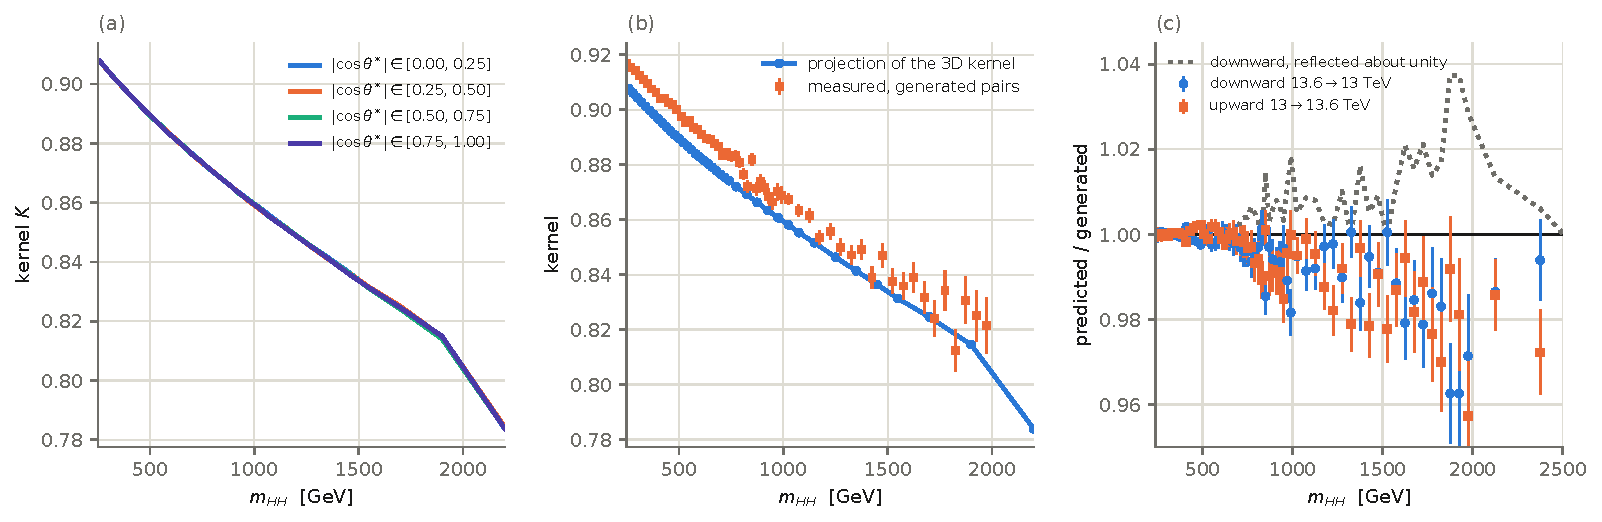
\includegraphics[width=\linewidth]{plots/energy_transport_checks.pdf}
\caption{\textcolor{red}{[AUTHORS ONLY]} Checks on the $13$~TeV transport.
(a) The per-bin kernel written into the coefficient file, split by $|\cos\theta^*|$.
(b) Its projection onto \mHH against the kernel measured from the 2784 generated pairs.
(c) The transport run in both directions over the same step in $\ln\sqrt{s}$, each
anchored on its own constant; the dotted curve is the downward result reflected about
unity.}
\label{fig:energy_checks}
\end{figure}

Panel (a) shows the kernel to be independent of $|\cos\theta^*|$ to within the line
width, so the transport is a function of \mHH alone at the present statistics. Panel (b)
shows its projection reproducing the independently measured kernel with the $1\%$ offset
quoted in Sec.~\ref{sec:energy_transport}. In panel (c) the overall constant inverts
between the two directions, $1.0098$ against $1/0.9902 = 1.0099$, while the per-bin
residual stays negative in both: anchored mean pulls are $-0.8$, $-1.2$, $-1.8$ and
$-0.6$ downward across the bands below $1$~TeV, $1$--$1.5$, $1.5$--$2$ and above
$2$~TeV, against $-0.4$, $-1.7$, $-1.8$ and $-2.5$ upward.

\clearpage
\subsection{\textcolor{red}{[AUTHORS ONLY]} Single-Higgs scaling with \texorpdfstring{$c_\PH$}{cH}: the implementation}
\label{sec:appendix_singleh}

\textcolor{red}{This subsection is for the authors and is not intended for the published
version. \textbf{Nothing in it is a new result.} Every curve here was produced with our
own implementation of scalings that already exist in the literature --- the $C_1$
coefficients and the $\kappa_\lambda$ dependence of single-Higgs production and decay
(Refs.~\cite{Degrassi:2016wml,Maltoni:2017ims}), including their use per STXS bin
(Refs.~\cite{ATLAS:2024lyh,Brivio:2022pyi}). The subsection exists for one purpose: to
let us check that our implementation reproduces what those references and the internal
CMS single-Higgs fits already give, before any of it is used. If a number here disagrees
with the literature, the implementation is wrong, not the literature. The two statements
that \emph{are} specific to this report --- the physical region of
$c_{\PH\mathrm{kin}}$ and the truncation of $\sigma\times\mathrm{BR}$ --- are in
Secs.~\ref{sec:trunc_singleh} and~\ref{sec:trunc_product}, and are not repeated here.}

The nine Wilson coefficients of Eq.~\eqref{eq:smeftpoint} also enter single-Higgs
production and decay, and a global fit constrains them with single-\PH and \HH data
together. Single-Higgs measurements are interpreted through the
STXS~\cite{Berger:2019wnu,deFlorian:2016spz}, bins in production
mode and a few kinematic variables, each parameterized as a polynomial in the Wilson
coefficients with a linear (interference) and a quadratic term, as in
Eq.~\eqref{eq:smeftpara_reorg}. The conventions and truncation options are those of
the LHC EFT Working Group~\cite{Brivio:2022pyi,Belvedere:2024nzh};
Ref.~\cite{ATLAS:2024lyh} carries the chain through on data.

These parameterizations are built from tree-level dimension-6 amplitudes, with QCD
corrections as $K$-factors. The operator $(\phi^\dagger\phi)^3$, whose coefficient
$c_\PH$ modifies the Higgs self-coupling, changes no single-Higgs vertex at tree
level: it enters only through the trilinear vertex in electroweak loop corrections.
The STXS parameterizations therefore have no $c_\PH$ term, and a combination with
\HH treats $c_\PH$ as constrained by \HH alone.

The dependence of single-Higgs rates on the ratio $\kappa_\lambda$ of the trilinear
coupling to its SM value is known at NLO in the electroweak couplings for the
inclusive cross sections~\cite{Degrassi:2016wml} and differentially for the main
production modes and decays~\cite{Maltoni:2017ims}. For a production mode and a
decay $i$,
\begin{equation}
\frac{\sigma}{\sigma_{\mathrm{SM}}}
= Z_\PH \left(1+\frac{(\kappa_\lambda-1)\,C_1}{K_{\mathrm{EW}}}\right),
\qquad
Z_\PH=\frac{1}{1-(\kappa_\lambda^2-1)\,\delta Z_\PH},
\qquad
\frac{\Gamma_i}{\Gamma_i^{\mathrm{SM}}} = 1+(\kappa_\lambda-1)\,C_1^{i},
\label{eq:c1master}
\end{equation}
with $\delta Z_\PH=-1.536\times10^{-3}$ a universal wave-function term, $C_1$ a
process-dependent coefficient and $K_{\mathrm{EW}}$ the NLO electroweak $K$-factor of
the mode. The branching ratios follow from the partial widths,
\begin{equation}
\frac{\mathrm{BR}_i}{\mathrm{BR}_i^{\mathrm{SM}}}
=\frac{\Gamma_i/\Gamma_i^{\mathrm{SM}}}
{\sum_j \mathrm{BR}_j^{\mathrm{SM}}\,\Gamma_j/\Gamma_j^{\mathrm{SM}}} .
\label{eq:brratio}
\end{equation}
The inclusive $C_1$ at $\sqrt{s}=13$~TeV are shown in Fig.~\ref{fig:c1values}
(left): production from Ref.~\cite{Degrassi:2016wml}, $\PQt\PH\PQq$ from
Ref.~\cite{Maltoni:2017ims}, decays from Ref.~\cite{Degrassi:2016wml} and
$\PZ\gamma$ from Ref.~\cite{Degrassi:2019yix}; the fermionic decays have $C_1=0$ at
this order.

The Wilson coefficients are mapped onto $\kappa_\lambda$ with the naive
translation between the HEFT self-coupling modifier and the Warsaw
basis~\cite{Alasfar:2023xpc},
Eq.~\eqref{eq:naivetranslation}
and Eq.~\eqref{eq:c1master} is evaluated at that $\kappa_\lambda$. With
$v=246.22$~GeV, $m_\PH=125$~GeV and $\Lambda=1$~TeV the coefficient of $c_\PH$ is
$-0.470$: $c_\PH=1$ gives $\kappa_\lambda=0.53$, and $c_\PH\in[-50,50]$ of
Table~\ref{tab:SMEFTcouplings} maps onto $\kappa_\lambda\in[-22.5,24.5]$
(Fig.~\ref{fig:c1values}, right). This adds one factor per process, depending on
$c_\PH$ and $c_{\PH\mathrm{kin}}$ only, on top of the STXS parameterization, and
requires no new simulation. The SMEFT single-Higgs model of Ref.~\cite{multihmodels}
implements it as a factor on the STXS scaling of each process, the production and
each partial width kept to first order in $\kappa_\lambda-1$ when the
parameterization is truncated at linear order. The \HH processes do not take it:
their $c_\PH$ dependence is part of the \HH parameterization of
Sec.~\ref{sec:parameterization}.

\begin{figure}[htp]
\centering
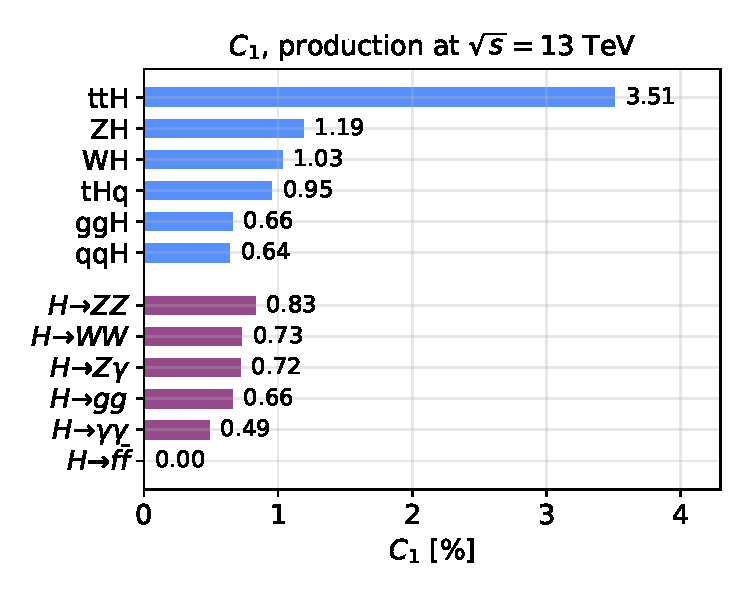
\includegraphics[width=0.49\textwidth]{single_higgs_ch/figures/c1_by_channel.pdf}
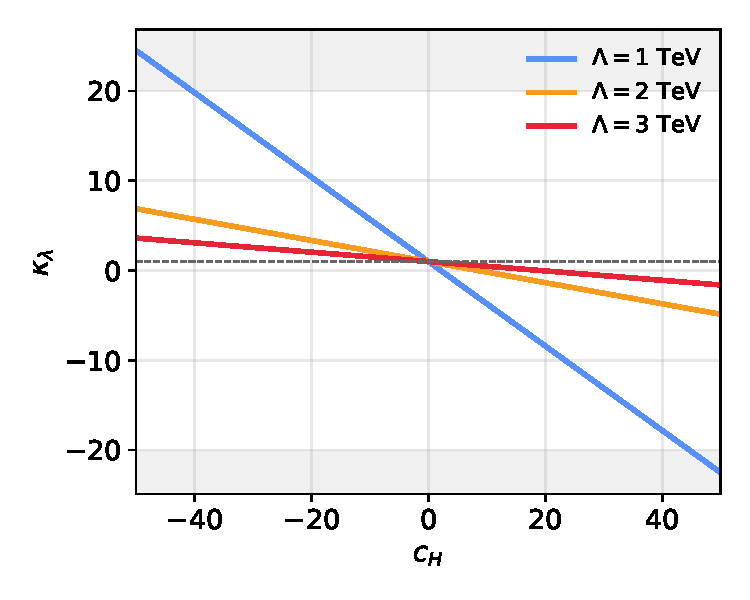
\includegraphics[width=0.49\textwidth]{single_higgs_ch/figures/kappa_lambda_vs_cH.pdf}
\caption{Left: inclusive $C_1$ coefficients of the single-Higgs production modes at
$\sqrt{s}=13$~TeV and of the Higgs
decays~\cite{Degrassi:2016wml,Maltoni:2017ims,Degrassi:2019yix}. Right: the naive
translation of Eq.~\eqref{eq:naivetranslation} from $c_\PH$ to $\kappa_\lambda$ for
three values of the EFT scale; the grey bands mark $|\kappa_\lambda|>20$. Both as in
the model of Ref.~\cite{multihmodels}.}
\label{fig:c1values}
\end{figure}

The translation has three limitations. $C_1$ is computed with only the trilinear

coupling rescaled; a consistent SMEFT calculation at the same order has further
one-loop contributions from the other operators, and operator mixing. An
$\mathcal{O}(\Lambda^{-2})$ coefficient enters a one-loop correction, so the result
is the leading self-coupling effect rather than a complete order in the EFT
expansion. Eq.~\eqref{eq:c1master} is quoted as valid for
$|\kappa_\lambda|<20$~\cite{Maltoni:2017ims}, $85\%$ of the $c_\PH$ range at
$\Lambda=1$~TeV, and the larger $|c_\PH|$ lie outside the region where the
dimension-6 truncation holds (Sec.~\ref{sec:truncation}).

The branching ratios change through the spread of $C_1^i$ across decays,
Eq.~\eqref{eq:brratio} (Fig.~\ref{fig:sh_br}). $\PQb\PAQb$ carries $58\%$ of the
width with $C_1=0$, so the fermionic branching ratios move opposite to the bosonic
ones: over the $c_\PH$ range, $\mathrm{BR}(\PZ\PZ)$ changes by up to $15\%$,
$\mathrm{BR}(\gamma\gamma)$ by $6\%$ and $\mathrm{BR}(\PQb\PAQb)$ by $6\%$ in the
opposite direction. $c_{\PH\mathrm{kin}}$, the coefficient of the Higgs
kinetic term, acts differently. Removing it by a field
redefinition rescales every single-Higgs coupling by the same factor, so that each
partial width scales as
Eq.~\eqref{eq:chkinwidth}
The rescaling cancels between the partial and the total width, and over the
$c_{\PH\mathrm{kin}}$ range of Table~\ref{tab:SMEFTcouplings} the branching ratios
change by less than $1\%$, only through the $c_{\PH\mathrm{kin}}$ term of
Eq.~\eqref{eq:naivetranslation}.

\begin{figure}[htp]
\centering
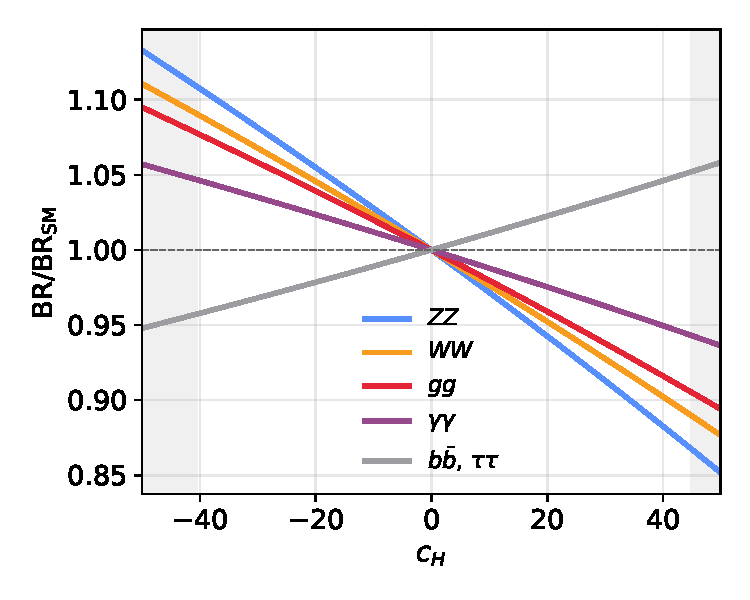
\includegraphics[width=0.49\textwidth]{single_higgs_ch/figures/br_ratio_vs_cH.pdf}
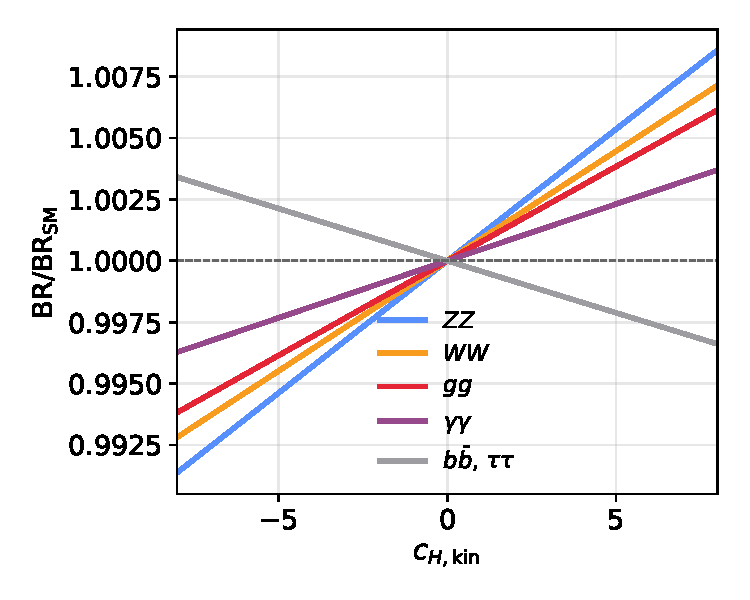
\includegraphics[width=0.49\textwidth]{single_higgs_ch/figures/br_ratio_vs_cHkin.pdf}
\caption{Higgs branching ratios normalized to their SM values as a function of
$c_\PH$ (left) and of $c_{\PH\mathrm{kin}}$ (right), at $\Lambda=1$~TeV;
$\tau\tau$ is identical to $\PQb\PAQb$. The grey bands on the left mark
$|\kappa_\lambda|>20$.}
\label{fig:sh_br}
\end{figure}


\begin{figure}[htp]
\centering
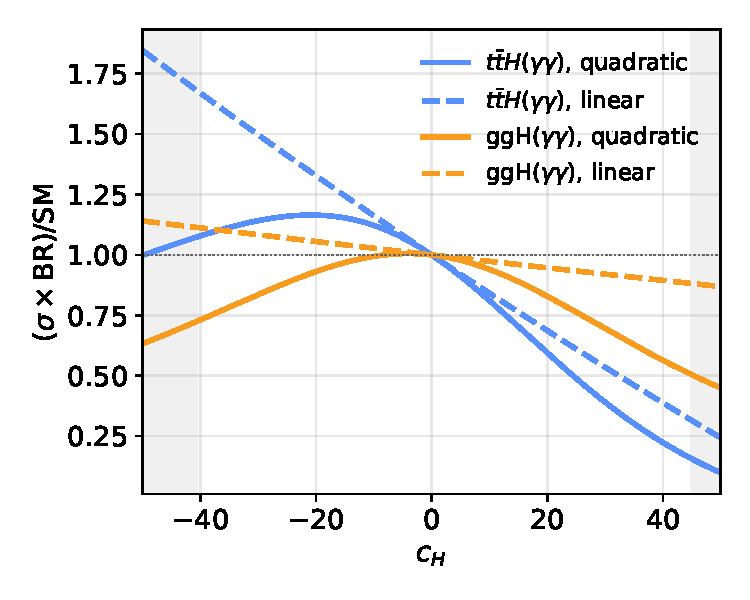
\includegraphics[width=0.52\textwidth]{single_higgs_ch/figures/sigma_times_br_vs_cH.pdf}
\caption{\textcolor{red}{[AUTHORS ONLY]} $\sigma\times\mathrm{BR}$ normalized to the SM for $\ttH(\gamma\gamma)$ and
$\ggH(\gamma\gamma)$, with the scaling of Eq.~\eqref{eq:c1master} in full (solid) and
truncated at first order in $\kappa_\lambda-1$ (dashed), as a function of $c_\PH$ at
$\sqrt{s}=13$~TeV and $\Lambda=1$~TeV, from the model of Ref.~\cite{multihmodels}; the
grey bands mark $|\kappa_\lambda|>20$.}
\label{fig:sh_rates}
\end{figure}

\paragraph{Dependence on the collision energy.}
\label{sec:singleh_ecm}

The decay coefficients $C_1^{i}$ are properties of the Higgs boson, so
Eq.~\eqref{eq:brratio} and the bound of Eq.~\eqref{eq:chkinbound} hold at every
energy. The production coefficients are tabulated at $7$, $8$, $13$ and
$14$~TeV~\cite{Degrassi:2016wml} and decrease slowly with energy ($3.87$, $3.78$,
$3.51$ and $3.47\%$ for \ttH). The model of Ref.~\cite{multihmodels} uses the
$13$~TeV values at $13.6$~TeV as well; the whole $13\to14$~TeV change is at most
$1.1\%$ relative. At $100$~TeV the production coefficients are not computed; their
evaluation requires the phase-space integration and parton-density convolution of
Refs.~\cite{Degrassi:2016wml,Maltoni:2017ims} redone at that energy.

At FCC-ee, at $\sqrt{s}=240$ and $365$~GeV~\cite{FCC:2018evy} and below the
$e^+e^-\to\PZ\HH$ threshold, $c_\PH$ is constrained only through the loop corrections
to $e^+e^-\to\PZ\PH$ and $\PGn\PAGn\PH$, the two energies separating the
self-coupling from the other Higgs couplings~\cite{DiVita:2017vrr}. The expected
precision is of order $30\%$ on $\kappa_\lambda$ from FCC-ee alone, better in
combination with the HL-LHC~\cite{Maura:2025fcc}, and its combination with \HH
requires both expressed in the same Wilson coefficients. Per unit $c_\PH$,
$e^+e^-\to\PZ\PH$ at $240$~GeV ($C_1\simeq1.5\%$~\cite{McCullough:2013ria}) is less
sensitive than \ttH (Fig.~\ref{fig:sh_fccee}); its weight comes from the precision of
the cross-section measurement. \textcolor{red}{\textbf{Oscar, Jon would you keep FCCee in
this paper? It would enrich discussion with not much work, but it is slightly off
topic.}}

\begin{figure}[htp]
\centering
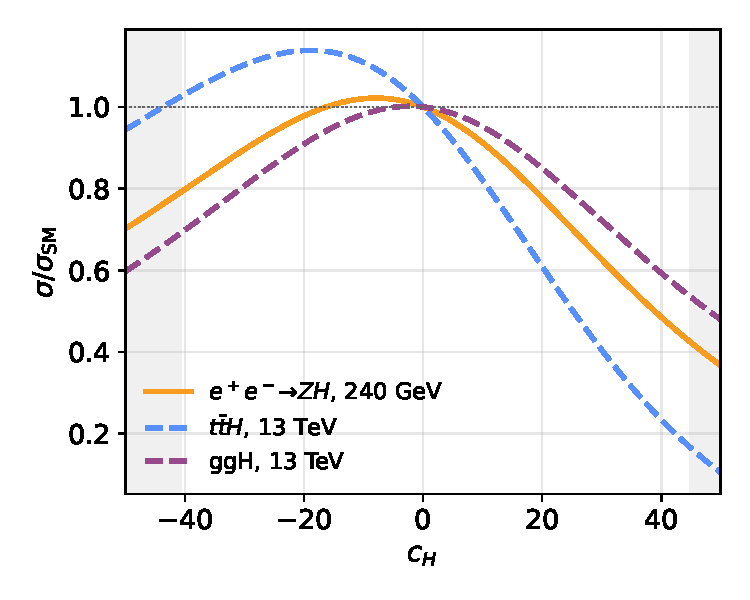
\includegraphics[width=0.62\textwidth]{single_higgs_ch/figures/fccee_vs_lhc_vs_cH.pdf}
\caption{Production cross sections normalized to their SM values as a function of
$c_\PH$ at $\Lambda=1$~TeV: $e^+e^-\to\PZ\PH$ at $\sqrt{s}=240$~GeV (solid), and \ttH
and \ggH at $\sqrt{s}=13$~TeV (dashed). The grey bands mark $|\kappa_\lambda|>20$.
\textcolor{red}{The $365$~GeV curves, and the $WW$-fusion channel, require $C_1$
values that are not yet filled in.} \textcolor{red}{\textbf{Jon, would you be able
to do?}}}
\label{fig:sh_fccee}
\end{figure}

At $\Lambda=1$~TeV a $5\%$ change of the inclusive \ttH rate requires $c_\PH\simeq3$,
small against the present experimental uncertainty on the \ttH cross section. The
term makes the parameterization consistent: $c_\PH$ enters both sides of the
combination, and its correlation with the coefficients \ttH constrains, notably
$c_{\PQt\PH}$, is propagated. With HL-LHC precision on \ttH and the differential
$C_1$ of Ref.~\cite{Maltoni:2017ims} the term becomes a constraint.

\textcolor{red}{TODO: cross-check the production curves against an explicit
\texttt{MG5\_aMC@NLO} evaluation and quote the residual scale and
$m_\PQt$-scheme uncertainty on $C_1$; extend to the differential level in
$p_{\mathrm{T}}^{\PH}$, where $C_1$ is enhanced at threshold; and decide whether
to commission a $100$~TeV computation of $C_1$ to match the reach of
Sec.~\ref{sec:extraction}.} \textcolor{red}{\textbf{Jon, would you be able to do?}}

\section{\textcolor{red}{[AUTHORS ONLY]} The basis for the linear truncation}
\label{sec:appendix_linear}
\label{sec:basis_linear}

\textcolor{red}{\textbf{MATHEUS:} this section records a basis that \emph{did not
work}, and is kept for us rather than for publication. The ten-point basis for the
truncated parametrisation is withdrawn: its basis points are themselves truncated
objects, and after the 4b selections four of the ten have a negative yield in the fully
merged region and one is negative everywhere while its inclusive cross section stays
positive. The ten points and `basis\_linear.txt` have been removed from multih-models
and `model\_linear` now uses the forty points with the formula truncated at evaluation
--- see `HANDOFF\_linear\_truncation\_via\_40point\_basis.md`. The linear-only 4b CSVs
built on the old ten labels need rebuilding or retiring.}

An analysis may choose to keep the effective-field-theory expansion only to the
interference term. That is a different parameterization --- ten monomials
rather than forty --- and it is solved on its own basis, given in
Table~\ref{tab:smeft_basis_linear}. The saving is ten simulated samples instead of forty.

Two points about using it. The coefficients are
\emph{not} obtained by fitting the ten-term system. They are the coefficients of
the full forty-term solve, restricted to the ten linear monomials, which are
$A_0$ to $A_4$ and $A_{15}$ to $A_{19}$ --- not the first ten. Truncating the
formula this way does reproduce samples generated with the same truncation;
fitting the truncated system directly does not. And the ten points of
Table~\ref{tab:smeft_basis_linear} are the basis of the truncated
parameterization, so they are to be used with the truncated formula and not
mixed with the forty points of Table~\ref{tab:smeft_basis_9d}.

The problem is easier than the quadratic one, and for a structural reason: every
monomial here involves at most \emph{one} coupling, where the quadratic
parameterization is two-local. The natural basis would then be the Standard
Model plus one single-coefficient point per coupling. That is not constructible
from the available grid, which has single-coefficient samples only for the four
four-fermion coefficients, so the same two-coupling restriction is applied; the
resulting basis is nevertheless well conditioned, $8.50$ against $32.7$ for the
forty-point one.

One pathology is specific to the truncation and has to be stated. The search
returns, if nothing prevents it, points whose \emph{truncated} total cross
section is negative --- two of ten, at $-598$ and $-39$~fb. Requiring a positive
total removes them, at a cost of $0.4\%$ in the score, which is inside the
seed-to-seed spread. The constraint acts on the total only, and the differential
prediction is not so easily repaired: six of the ten points have negative bins,
between $8$ and $29$ of the $40$, and four of them predict a negative yield
above $1$~TeV. Whether that matters is a question about the analysis rather than
about the basis, and it is taken up in
Sec.~\ref{sec:validation_realistic}.

% generated by scripts/make_basis_table.py in the basis-optimization toolkit; do not edit by hand
\begin{table}[htbp]
\centering\scriptsize
\begin{tabular}{l p{0.38\textwidth} r}
\hline
Point & Non-zero coefficients & $\sigma$ [fb] \\
\hline
BP 01 & SM (all zero) & $31.01$ \\
BP 02 & $c_{\PQt G} = 1$,\; $c_{Q\PQt}^{(1)} = -20$ & $7.238$ \\
BP 03 & $c_{\PQt G} = 1$,\; $c_{Q\PQt}^{(1)} = 20$ & $9.377$ \\
BP 04 & $c_{Q\PQt}^{(8)} = -20$,\; $c_{QQ}^{(8)} = 20$ & $34.44$ \\
BP 05 & $c_{Q\PQt}^{(8)} = -20$,\; $c_{QQ\PQt\PQt} = 20$ & $34.54$ \\
BP 06 & $c_{QQ\PQt\PQt} = 20$,\; $c_{QQ}^{(8)} = 20$ & $31.16$ \\
BP 07 & $c_{\PH\mathrm{kin}} = -8$,\; $c_{\PH G} = -0.1$ & $178.4$ \\
BP 08 & $c_{\PQt\PH} = -10$,\; $c_{\PH G} = -0.0567$ & $4.938$ \\
BP 09 & $c_{\PH} = 50$,\; $c_{\PH G} = -0.0856$ & $742.3$ \\
BP 10 & $c_{\PH\mathrm{kin}} = 8$,\; $c_{\PH G} = -0.1$ & $68.6$ \\
\hline
\end{tabular}
\caption{The ten points of the basis for the linear truncation. Only the coefficients that differ from zero are listed; all others vanish. Every point other than the SM activates exactly two coefficients. Cross sections are evaluated from the inclusive coefficients of the reweighting fit, restricted to the ten linear monomials.}
\label{tab:smeft_basis_linear}
\end{table}


Fig.~\ref{fig:basis_shapes_linear} shows the \mHH distribution of each of the
ten points, normalized to its own yield, in the same format as
Fig.~\ref{fig:basis_shapes}. The contrast with the forty-point basis is the
point of showing it. There, the points fall into four kinematic regimes and the
fraction of the yield above $1$~TeV spans $0.8\%$ to $18\%$. Here all ten
classify as SM-like, and the same fraction runs from $3.3\%$ down to
$-56\%$: the truncated prediction has no access to the hard-tail regime, and
where the interference exceeds the SM term it goes negative rather
than small. This is a property of the truncation and not of the basis --- the
points themselves reach $c_\PH=50$ --- and it is the reason the usability
question of Sec.~\ref{sec:validation_realistic} is posed in terms of the
observable being fitted.

\begin{figure}[htbp]
    \centering
    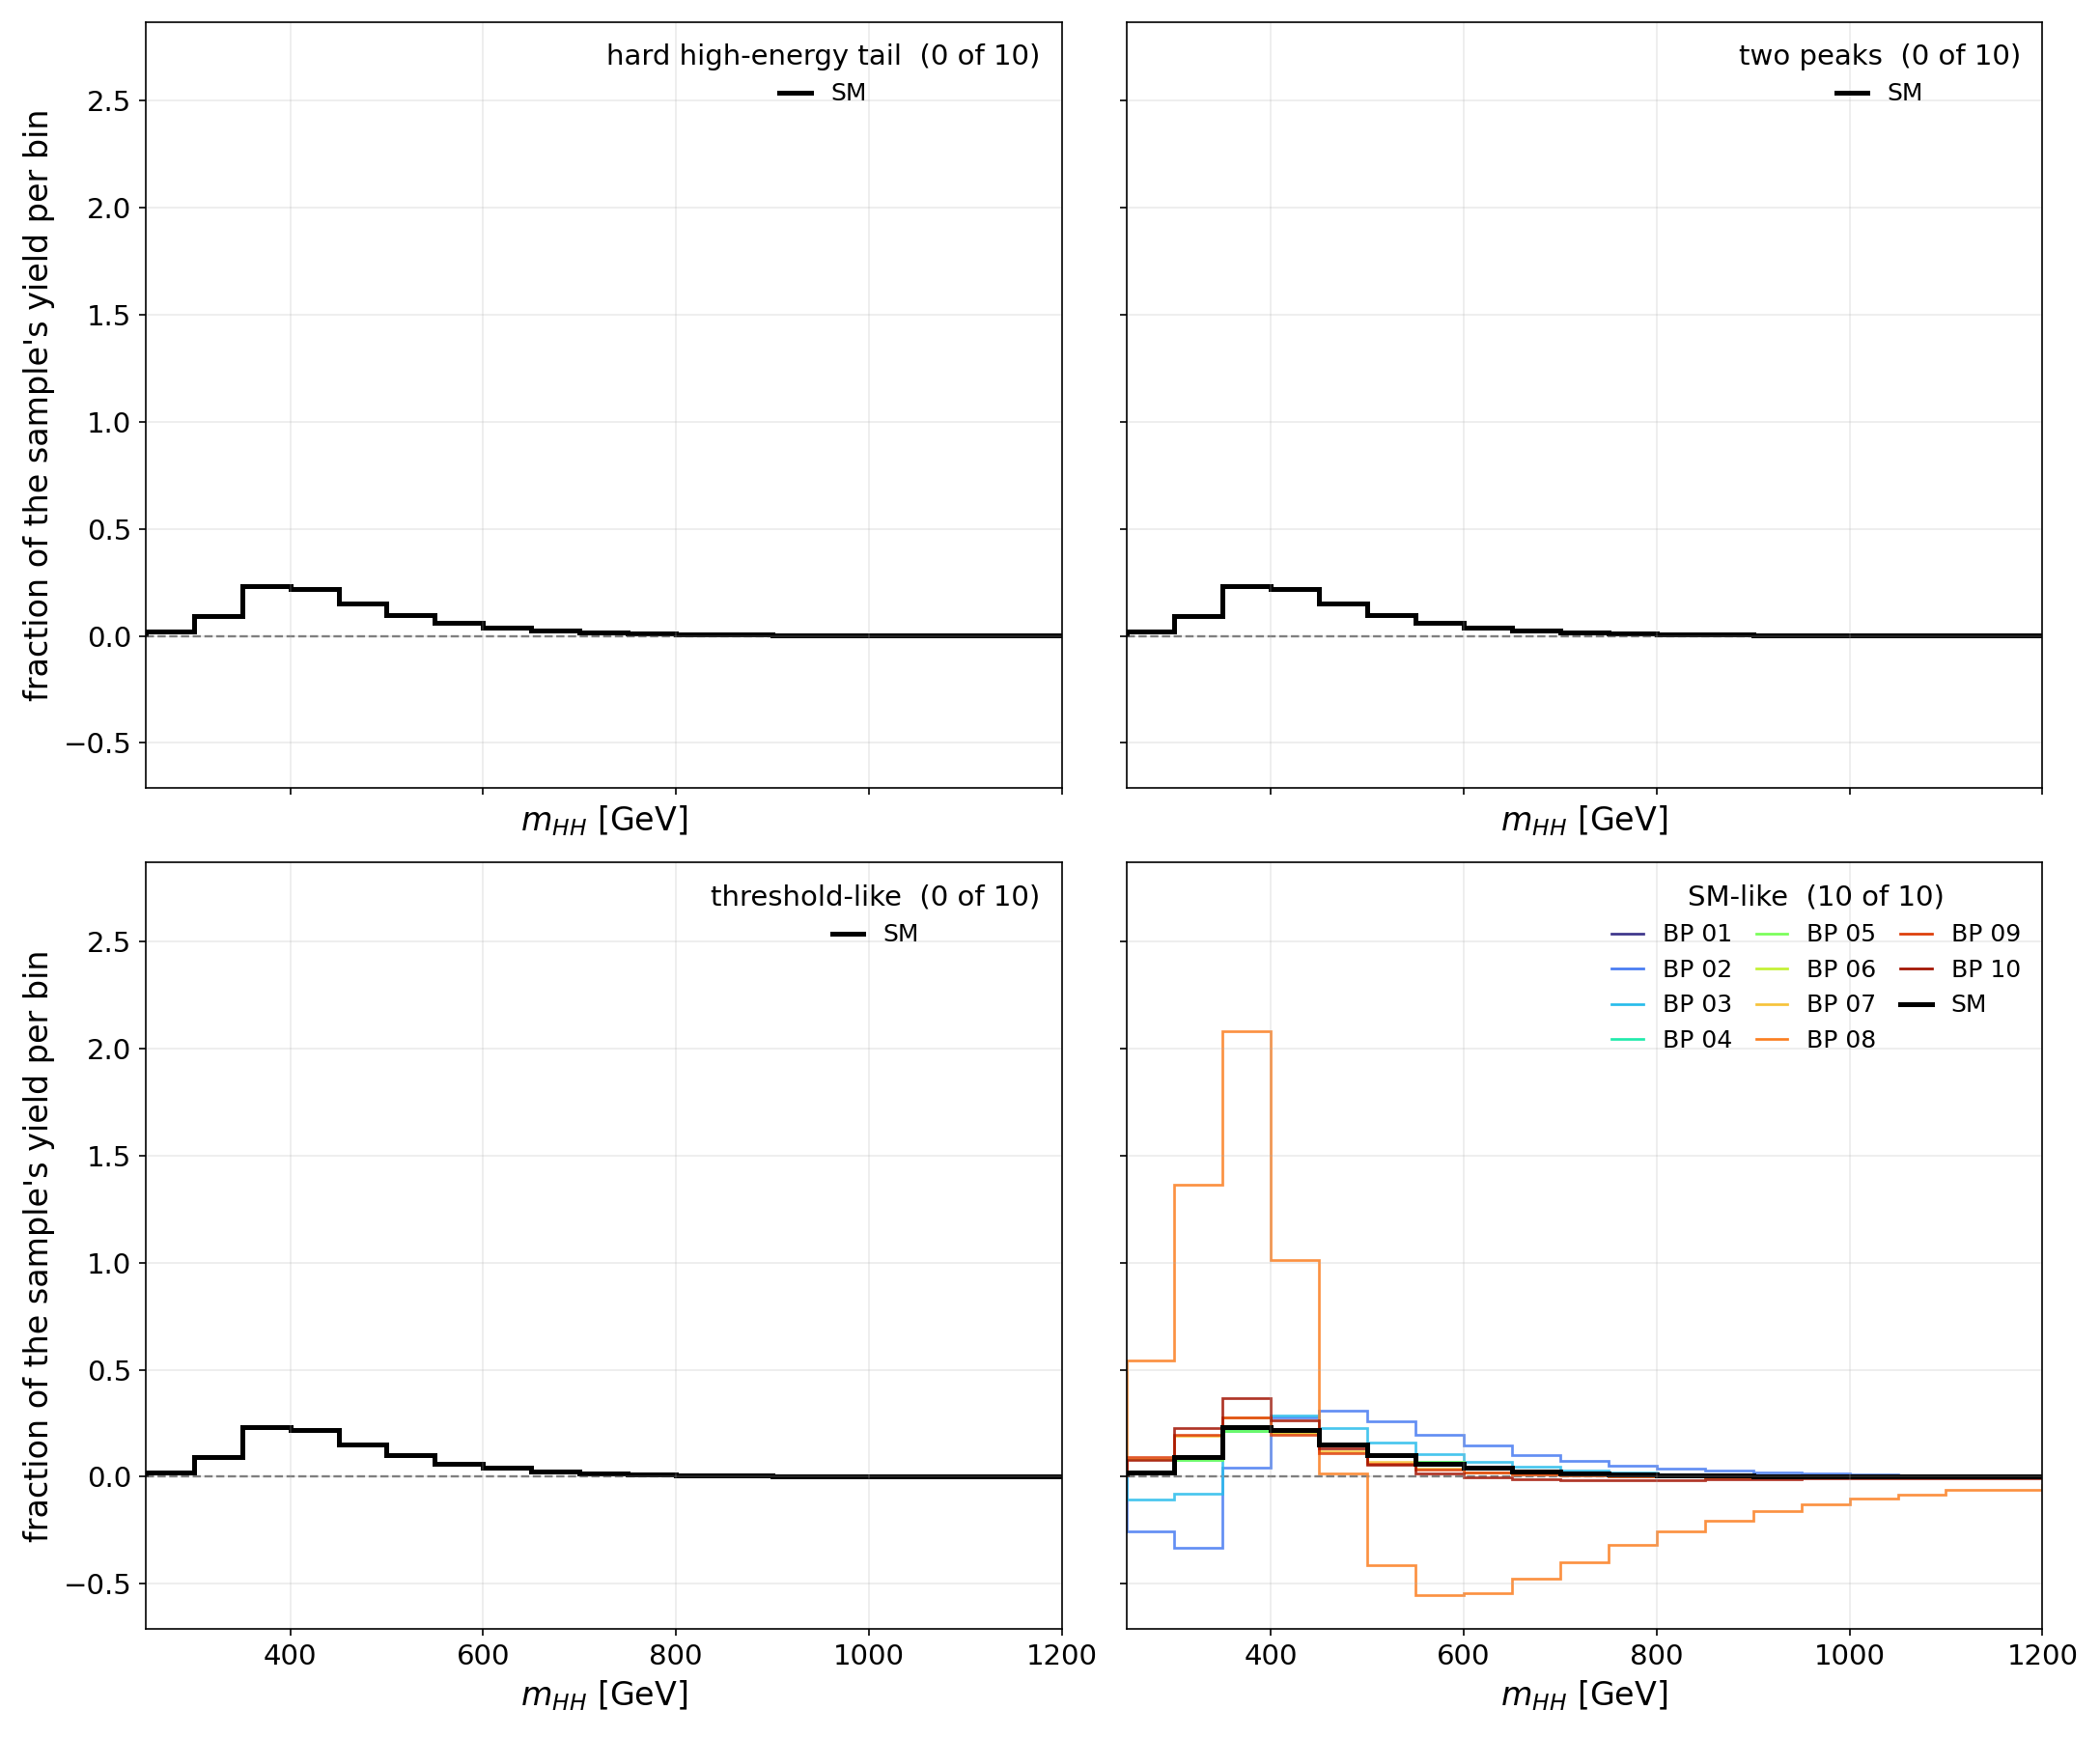
\includegraphics[width=0.70\textwidth]
        {figures/basis_optimization/basis_shapes_linear.png}
    \caption{Normalized \mHH distribution of each of the ten points of the
    linear basis, with the SM drawn in black. Each histogram is
    divided by its own integral. Bins in which the truncated prediction is
    negative are drawn as such; the dashed line marks zero.}
    \label{fig:basis_shapes_linear}
\end{figure}

Fig.~\ref{fig:basis_convergence_linear} shows the search, every seed of the
sweep. It converges far more readily than the quadratic one: the final score
spreads by a factor $1.09$ over the seeds, against $1.34$ for the forty-point
basis, and a seed accepts a median of $13$ exchanges against $91$. Both follow
from the candidate set being small --- the positive-total requirement and the
two-coupling restriction leave $1135$ of the $4376$ pool samples --- and from
the ten-term system being easier to span. The practical consequence is that the
sweep matters less here than it does for the quadratic basis, where it is part
of the procedure.

\begin{figure}[htbp]
    \centering
    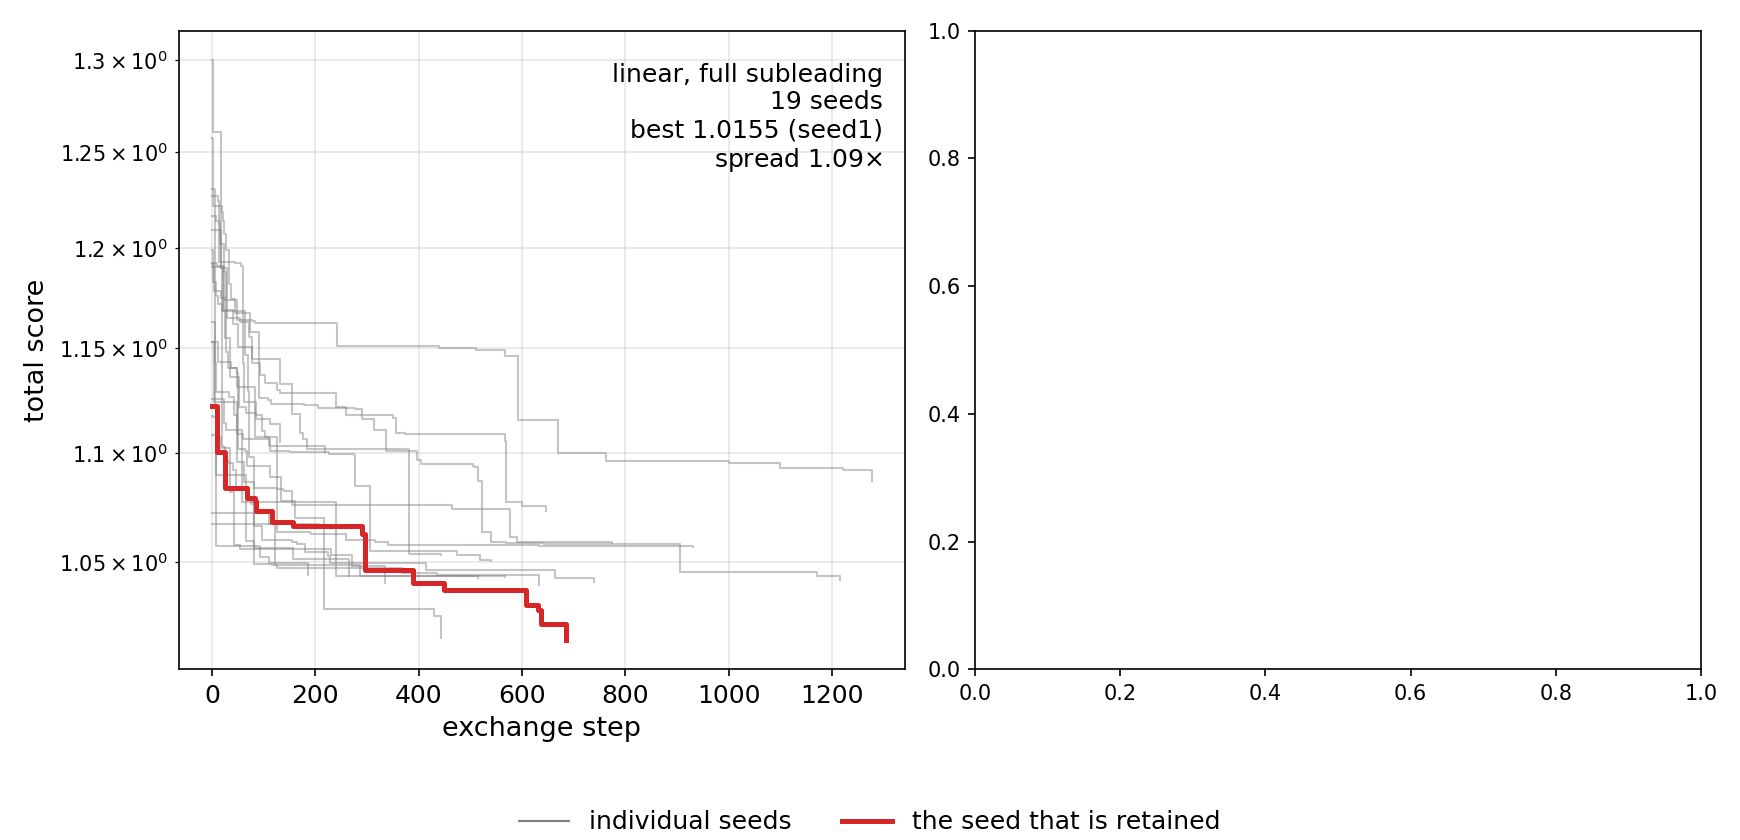
\includegraphics[width=0.60\textwidth]
        {figures/basis_optimization/basis_convergence_linear.png}
    \caption{Total score against exchange step for every seed of the linear
    basis search; the retained seed is highlighted.}
    \label{fig:basis_convergence_linear}
\end{figure}

\subsection{The linear truncation after a selection}
\label{sec:appendix_linear_selection}
The ten points of Sec.~\ref{sec:basis_linear} exist so that an analysis
truncating at the interference term can do so with ten samples instead of
forty. Whether that is a saving or a false economy is a question only this
section can answer, because it depends on what is being fitted and on which
part of phase space is kept.

Without any selection the truncated templates are already difficult: six of the
ten basis points have between $8$ and $29$ negative bins of $40$, and four
predict a negative yield above $1$~TeV, even though the positivity constraint
imposed during the search keeps every inclusive total positive. Where the
interference term exceeds the SM one the truncated cross section
goes negative rather than small. A fit to a rate need not notice; a fit to a
shape cannot use a template that is negative in most of its bins.

After a selection the bin-level problem does not go away,
it only moves: in the binning the datacard actually uses, six of the ten
templates still have negative bins, between two and twelve of twenty-three. Beyond that, the problem stops being about individual bins at all. Of the ten points, four have a
negative yield in the merged selection, and one --- the
point at $c_{\PQt\PH}=-10$, $c_{\PH G}=-0.0567$ --- is negative in every region
while its truncated inclusive cross section is positive. That is not a template
with awkward bins: its integral is negative, so it can enter a fit neither as a
shape nor as a rate.

The reason is that the positivity constraint acts on the inclusive total, and
inclusive positivity does not survive a selection. A selection reweights the
bins, and one that favours the high-mass tail concentrates exactly the region
where the truncated prediction is most negative. A constraint that would help
has to impose positivity after the analysis's own selection, which a basis
search cannot do in advance because it does not know the selection.

The conclusion is that the ten-point basis is not usable with these selections,
and the question is not whether a shape fit can use the templates but whether a
usable linear basis exists for a given selection at all. Two routes remain. An
analysis restricting its coupling ranges may not meet the problem, since every
negative point lies far from the SM. Otherwise the forty-point
basis with the formula truncated at evaluation time gives a linear prediction
with no negative templates; it is a different object and costs forty samples
rather than ten, and the two are not interchangeable.

\clearpage
\subsection{\textcolor{red}{[AUTHORS ONLY]} The dimension-6 validity criterion, per operator and per bin}
\label{sec:appendix_trunc_validity}

\textcolor{red}{For the authors. The criterion itself is not ours --- restricting to where
the interference dominates the dimension-6 square is the standard prescription, and the
threshold is a convention with no first-principles answer~\cite{Contino:2016jqw,Brivio:2017vri}. What is
ours is the evaluation below: the same criterion applied to the nine coefficients of this
report, differentially in \mHH rather than inclusively, from the fitted
$A$-coefficients. It is kept here rather than in the main text because it supports a
statement the literature already makes, and because the numbers depend on a threshold we
chose.}

\begin{table}[htbp]
\centering
\begin{tabular}{l|cccc}
\hline
operator & inclusive & $\mHH \in [400,410]$~GeV & $\mHH \in [1000,1050]$~GeV & $\mHH \in [1400,1500]$~GeV \\
\hline
$c_{\PH}$              & $5.6$ & $9$ & $21.5$ & $28.4$ \\
$c_{\PH\mathrm{kin}}$  & $7.8$ & $13.9$ & $3.02$ & $1.63$ \\
$c_{\PQt\PH}$          & $7.21$ & $13.4$ & $2.25$ & $1.27$ \\
$c_{\PH G}$            & $0.0263$ & $0.0754$ & $0.0092$ & $0.00591$ \\
\hline
\end{tabular}
\caption{\textcolor{red}{[AUTHORS ONLY]} Coupling value $|c|\simeq|A^j_{\text{lin}}/A^j_{\text{quad}}|$ at which the
dimension-6 squared contribution equals the dimension-6 interference, for the four
leading operators, inclusively and in three \mHH bins, at $\sqrt{s}=13.6$~TeV.
$A^j_{\text{quad}}$ is the diagonal entry of the leading quadratic block. The quantity
is defined only for operators with a genuine square.}
\label{tab:trunc_validity}
\end{table}

\clearpage
\section{Details of the basis search}
\label{sec:appendix_basis_search}

The search is that of Ref.~\cite{HH_nonggf_R5}; this appendix gives the five
implementation changes summarized in Sec.~\ref{sec:basis_refinements}, the arguments for
restricting the basis to the planes, and the changes that were tried and did not improve
the result.

\subsection{Why the basis is restricted to the planes}
\label{sec:appendix_basis_planes}

The result is in Sec.~\ref{sec:basis_planes}; the arguments for it are collected here.

The sample grids of Sec.~\ref{sec:grids} are not an unstructured cloud: most of
their points lie in one of the $\binom{9}{2}$ planes in which a single pair of
Wilson coefficients is varied with the rest held at their SM values.
We exploit that structure and require the basis points to be drawn from those
planes, allowing a small number of exceptions.

The restriction is not an approximation. No monomial of
Eq.~\eqref{eq:smeftpara_reorg} involves more than two distinct coefficients: the
$40$ terms are the SM term, the linear terms, the pairwise-quadratic
combinations of the four leading coefficients, and the products of one leading
with one subleading coefficient. The parameterisation is in this sense
\emph{two-local}, and a set of points each of which activates at most two
coefficients is therefore not structurally degenerate.

Two considerations motivate the choice. The first is numerical. Bases selected
from the planes are consistently better conditioned than bases selected from the
whole pool --- condition number $21$ against $33$ for the $20$-point 5D basis,
and $26$ against $40$ for the $40$-point 9D one --- because points that activate
many coefficients at once populate the monomials less distinctly and bring the
basis closer to degeneracy. The second is interpretational. Every basis point
then isolates one coefficient pair, so each template can be attributed to a
specific pair of operators, and the basis maps directly onto the
two-dimensional scans in which the results of such analyses are presented.

The restriction was initially applied with a budget of a few exceptions, on the
expectation that it would not be free: a basis drawn only from the planes might
be more accurate on plane targets and less accurate on the rest, and the points
that activate many coefficients make up the majority of the sample set. That
expectation turned out to be wrong, and the budget is not used.

Only the \emph{membership} of the basis is restricted. The
validation targets against which every candidate basis is scored are never restricted:
the loss asks a candidate to predict every other sample in the grid, and at $13.6$~TeV
$2792$ of the $4376$ samples --- about two thirds --- activate more than two
coefficients. The basis is therefore always required to describe the full parameter
space, and is selected on its ability to do so; what is structured is only the set of
points it may be built from.

Scoring the twenty converged seeds against on-plane targets alone and against
off-plane targets alone gives rankings with a Spearman correlation of $0.24$: the basis
that is best on the planes ranks sixteenth of twenty off them, while the basis adopted
here is first off the planes and third on them. Off the planes the interpolation error
and the morphing weight norms are both about $1.6$ times larger. A grid of plane scans
alone would therefore determine the coefficients, but would not discriminate between
candidate bases.

The full sweep settles it. Every one of the $40$ points of the recommended
nine-coefficient basis lies in a two-dimensional plane: thirty-nine activate
exactly two coefficients and one is the SM. Its condition number is
$32.7$ and its total score $0.609$, against $18.4$ and $0.359$ for the
twenty-point basis and $12.7$ and $0.305$ for the fifteen-point one; the score is
not comparable between parameterizations of different size, since it is dominated
by terms that grow with the number of monomials. Allowing two points off the
planes was tested on the same footing, as a separate twenty-seed sweep: it gives
a slightly worse score ($0.624$) and a measurably worse closure against the
generated samples ($3.5\%$ against $3.0\%$ in median relative shape residual,
Sec.~\ref{sec:validation_mm}), at a slightly better condition number ($26.6$).
The restriction therefore costs nothing in accuracy, and every basis point lies in a
plane the results are presented in.

\subsection{Refinements to the search, and what did not improve it}
\label{sec:appendix_basis_refinements}
\label{sec:basis_difficulty}

Five changes with respect to the search of Ref.~\cite{HH_nonggf_R5}:

\begin{itemize}
  \item \emph{Degeneracy of randomly drawn starting configurations.} Ref.~\cite{HH_nonggf_R5} initializes each seed from the best of several starting configurations, one of which is a set of purely random selections. In nine dimensions a randomly drawn configuration is almost always singular, for a counting reason rather than through bad luck. Of the $40$ monomials of Eq.~\eqref{eq:smeftpara_reorg}, $20$ vanish unless one of the four four-fermion coefficients is non-zero, while only $45\%$ of the generated samples have one; a uniform draw of $40$ points therefore contains about $18$ such samples where $20$ are needed, and we find that $85\%$ of random draws give a rank-deficient interpolation matrix. The random starting configurations are accordingly redrawn until the matrix has full rank, which restores all of them to use. The effect is absent at the dimensionality of Ref.~\cite{HH_nonggf_R5}, where the corresponding fraction is negligible, and it grows with the number of coefficients that enter the parameterization only through products.
  \item \emph{Rank in the well-conditioned starting configuration.} The second starting configuration of Ref.~\cite{HH_nonggf_R5} is the one that favours well-conditioned interpolation matrices, built greedily by adding at each step the sample that most increases the pseudo-determinant. Ranking candidates by the pseudo-determinant alone is not safe when the matrix is still rank deficient: discarding a vanishing singular value increases the product over the surviving ones, so a selection that keeps the matrix degenerate can score higher than one that does not. We therefore rank candidates first by the rank of the matrix and only then by the pseudo-determinant. The two orderings agree whenever the candidate samples are unstructured, which is why this does not affect the bases of Ref.~\cite{HH_nonggf_R5}; they differ when the candidates are restricted, as they are by the two-dimensional plane requirement of Sec.~\ref{sec:basis_planes}, where the unmodified ranking returns a basis one short of full rank even when every candidate is examined.
  \item \emph{Validation targets.} Ref.~\cite{HH_nonggf_R5} evaluates every candidate basis against every sample of the optimization set. Preserving that at the sample sizes of this report is a question of implementation rather than of method: evaluating the score for all targets at once, rather than one target at a time, reduces its cost by a factor of about five and keeps the full optimization set affordable at every exchange step. No subsampling of the targets is therefore used, and the scores quoted here are computed on the complete set.
  \item \emph{Number of basis points.} The bases of Ref.~\cite{HH_nonggf_R5} are exactly determined: as many samples as coupling structures, so that the interpolation matrix is square and inverted exactly. We retain that as the default and allow, as an option, more samples than structures. The interpolation weights are then the minimum-norm least-squares solution, which distributes the weight of a target over more samples and so averages down the statistical uncertainty each of them carries. This is the unweighted counterpart of the statistically aware extension of Ref.~\cite{HHMatrix_R5}: it spreads the weights but treats every sample as equally reliable, whereas Ref.~\cite{HHMatrix_R5} weights them by their covariance. Recovering the full procedure requires per-bin uncertainties to be propagated with the samples. The bases reported here are all exactly determined.
  \item \emph{Recording the convergence.} Ref.~\cite{HH_nonggf_R5} notes in its appendix that the step-by-step trace of the published runs was written only to the standard output of the batch jobs and did not survive with the results, so that no convergence information could be reported. The optimization used here writes the accepted exchanges and the value of every term of the score to a file as the search proceeds, so a run that is interrupted still leaves its convergence behind.
\end{itemize}

Figure~\ref{fig:basis_convergence} shows those trajectories for the two ends of the
ladder, every seed of each. Three things follow. The descent is fast and then stops: by
step $50$ a seed has already made $90\%$ of the total improvement it will ever make for
the fifteen-point basis, and $83\%$ for the forty-point one. The seeds do not converge
to a common value, and the spread of their final scores is far larger than the few per
cent of improvement still available after step $200$: they differ not in how far they
descend but in which local optimum they reach, which is also why the starting
configuration does not predict the outcome (the rank correlation between initial and
final score is $+0.08$ and $+0.22$). And a seed cannot be judged early: ranking the
seeds by their score at step $50$ has rank correlation $-0.09$ and $-0.11$ with their
final ranking, and at step $200$, with most of the improvement already banked, still
only $+0.45$ and $-0.06$. Starting many seeds, keeping the best few and letting only
those finish would therefore select close to at random for the nominal basis: the
ordering is settled in the long, nearly flat tail of the trajectory, where little score
is gained but the basis is still being rearranged. Every seed is run to its own
stopping rule.

\begin{figure}[htbp]
    \centering
    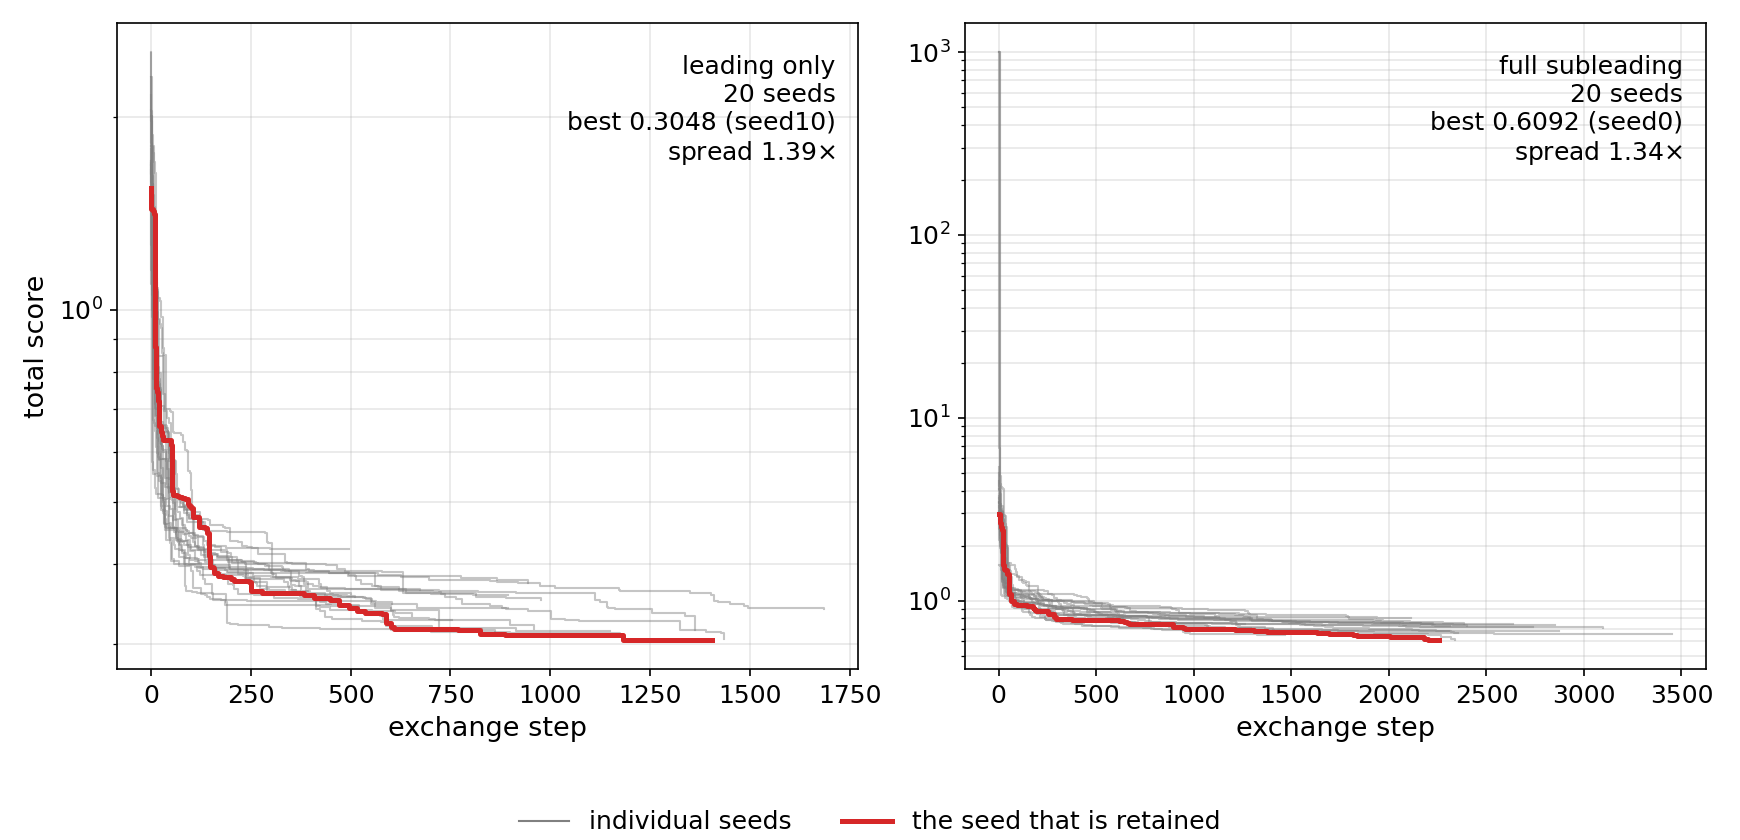
\includegraphics[width=0.92\textwidth]
        {figures/basis_optimization/basis_convergence.png}
    \caption{Total score against exchange step for each of the $20$ seeds of the
    fifteen-point (left) and forty-point (right) optimizations; the seed that is
    retained is highlighted. Each line is a staircase of accepted exchanges, taken from
    the record the search writes as it proceeds. Only accepted exchanges appear as
    steps, so the flat stretches are not idle: each step probes $30$ candidate
    replacements. The score is not comparable between the two panels, being dominated
    by terms that grow with the number of monomials.}
    \label{fig:basis_convergence}
\end{figure}

Each parameterization was optimized with $20$ independent seeds. The searches accept a
median of $47$ exchanges and stop after $300$ consecutive steps without an improvement.
The spread of the final score over seeds is a factor $1.39$, $1.31$ and $1.34$ for the
fifteen-, twenty- and forty-point cases, so one run does not determine the basis and
the sweep is part of the procedure.

Four further changes were tried and did not improve the result:

\begin{itemize}
  \item \emph{Penalizing the norm of the interpolation weights.} The residual of
    the matrix method is dominated by the statistical error of the basis samples
    propagated through those weights, so penalizing their quadratic norm appears
    to address the dominant term directly. It does not: over the seeds of the
    nine-coefficient sweep the norm is weakly \emph{anti}-correlated with the
    delivered residual (Spearman $-0.18$), and selecting on it gives $4.2\%$
    against the $3.5\%$ of the score. The term is used only for the truncated
    parameterizations, where the closure terms vanish identically and the weight
    norms are the only quantity that varies between bases.
  \item \emph{Selecting the seed on the validation rather than on the score.}
    This does improve the median residual, by $24\%$, $3\%$ and $13\%$ for the
    three parameterizations, but it degrades the tail where the two disagree: for
    the nominal basis the $99$th percentile worsens from $0.21$ to $0.24$. The
    score is weighted towards the worst case, so the two criteria answer different
    questions. We retain the score, and quote the validation separately in
    Sec.~\ref{sec:validation}.
  \item \emph{Over-determined bases.} An optimized exactly-determined basis was the
    better of the two at equal cost, and the same statistical gain is obtained more
    effectively by building the basis points from a few samples by reweighting
    (Sec.~\ref{sec:validation_nsamples}).
  \item \emph{Exhausting the neighbourhood before stopping.} The search stops
    after $300$ steps without an improvement rather than after proving that no
    single exchange improves. An exhaustive sweep of the $8520$ single-exchange
    neighbours of a converged basis found four improving moves, the best of them
    $1.5\%$ of the score, and that move left the median residual unchanged.
    The stopping rule is therefore not what limits the result.
\end{itemize}

The basis is optimized at $\sqrt{s}=13.6$~TeV, the main energy of this report. Since the \ggHH kinematics at $13$~TeV are very close to those at $13.6$~TeV, the same basis is applicable there without being re-optimized. \textcolor{red}{PLACEHOLDER: at $100$~TeV the kinematics change substantially, the spectrum extending to much higher \mHH and the relative weight of the diagrams shifting accordingly; we still have to see how much the basis is affected and whether the matrix method, with a basis optimized in this way, is applicable at that energy at all. The ELR coefficients are in any case provided at $100$~TeV.}

The resulting basis for the nominal nine-coefficient parameterization is given in
Table~\ref{tab:smeft_basis_9d}. It is the default of this report; the bases of the
two reduced parameterizations are used only for the comparisons of
Sec.~\ref{sec:validation} and are not reproduced here.

% Generated by scripts/make_basis_table.py in the basis-optimization toolkit
% (--layout sparse). The dense nine-column layout the script can also produce is
% not used: every point activates exactly two coefficients, so seven of the nine
% columns would be zero on every row.
% generated by scripts/make_basis_table.py in the basis-optimization toolkit; do not edit by hand
%\begin{table}[htbp]
%\centering\scriptsize
%\begin{tabular}{l p{0.26\textwidth} r|l p{0.26\textwidth} r}
%\hline
%Point & Non-zero coefficients & $\sigma$ [fb] & Point & Non-zero coefficients & $\sigma$ [fb] \\
%\hline
%BP 01 & SM (all zero) & $31.01$ & BP 21 & $c_{\PH\mathrm{kin}} = -8$,\; $c_{QQ\PQt\PQt} = -20$ & $141.7$ \\
%BP 02 & $c_{\PH G} = -0.0567$,\; $c_{\PQt G} = 1$ & $120.9$ & BP 22 & $c_{\PH} = -27.8$,\; $c_{QQ}^{(8)} = -20$ & $1424$ \\
%BP 03 & $c_{\PH G} = -0.0711$,\; $c_{QQ}^{(8)} = 20$ & $274.7$ & BP 23 & $c_{\PH} = -27.8$,\; $c_{\PH\mathrm{kin}} = -2.67$ & $1264$ \\
%BP 04 & $c_{\PH G} = -0.0856$,\; $c_{Q\PQt}^{(1)} = -20$ & $346.6$ & BP 24 & $c_{u\PH} = 7$,\; $c_{QQ\PQt\PQt} = -10$ & $139.1$ \\
%BP 05 & $c_{\PH G} = -0.1$,\; $c_{Q\PQt}^{(1)} = 10$ & $486.7$ & BP 25 & $c_{\PH\mathrm{kin}} = 8$,\; $c_{u\PH} = -10$ & $210.5$ \\
%BP 06 & $c_{\PH G} = -0.1$,\; $c_{QQ\PQt\PQt} = -10$ & $473.8$ & BP 26 & $c_{\PH\mathrm{kin}} = 8$,\; $c_{QQ\PQt\PQt} = 20$ & $32.18$ \\
%BP 07 & $c_{\PH\mathrm{kin}} = 8$,\; $c_{\PQt G} = 1$ & $47.94$ & BP 27 & $c_{u\PH} = 1.33$,\; $c_{Q\PQt}^{(8)} = -20$ & $47.06$ \\
%BP 08 & $c_{\PH\mathrm{kin}} = 8$,\; $c_{\PH G} = -0.0711$ & $110.7$ & BP 28 & $c_{\PH G} = -0.0711$,\; $c_{Q\PQt}^{(8)} = -20$ & $269.7$ \\
%BP 09 & $c_{u\PH} = -8.11$,\; $c_{\PQt G} = 0.675$ & $48.25$ & BP 29 & $c_{\PH} = -16.7$,\; $c_{\PQt G} = 0.675$ & $521.6$ \\
%BP 10 & $c_{\PH} = -50$,\; $c_{QQ\PQt\PQt} = -20$ & $5050$ & BP 30 & $c_{u\PH} = -10$,\; $c_{Q\PQt}^{(1)} = -20$ & $66.08$ \\
%BP 11 & $c_{u\PH} = 7$,\; $c_{QQ\PQt\PQt} = 10$ & $139.5$ & BP 31 & $c_{\PH} = 38.9$,\; $c_{QQ\PQt\PQt} = -10$ & $3939$ \\
%BP 12 & $c_{u\PH} = -8.11$,\; $c_{\PH G} = -0.0856$ & $177.3$ & BP 32 & $c_{\PH\mathrm{kin}} = 4.44$,\; $c_{QQ\PQt\PQt} = -20$ & $17.95$ \\
%BP 13 & $c_{\PH} = -38.9$,\; $c_{\PH G} = -0.1$ & $1764$ & BP 33 & $c_{\PH} = -38.9$,\; $c_{\PH\mathrm{kin}} = 6.22$ & $3550$ \\
%BP 14 & $c_{\PH} = -27.8$,\; $c_{Q\PQt}^{(1)} = 20$ & $1391$ & BP 34 & $c_{\PQt G} = 1$,\; $c_{QQ}^{(8)} = -20$ & $8.282$ \\
%BP 15 & $c_{u\PH} = -10$,\; $c_{Q\PQt}^{(1)} = 20$ & $56.78$ & BP 35 & $c_{\PQt G} = 1$,\; $c_{QQ}^{(8)} = 20$ & $8.334$ \\
%BP 16 & $c_{u\PH} = -8.11$,\; $c_{Q\PQt}^{(8)} = -20$ & $40.9$ & BP 36 & $c_{\PH\mathrm{kin}} = -8$,\; $c_{QQ}^{(8)} = -20$ & $142.1$ \\
%BP 17 & $c_{\PH\mathrm{kin}} = -8$,\; $c_{Q\PQt}^{(1)} = 10$ & $145.7$ & BP 37 & $c_{\PH\mathrm{kin}} = 6.22$,\; $c_{Q\PQt}^{(8)} = -20$ & $25.65$ \\
%BP 18 & $c_{\PH\mathrm{kin}} = -8$,\; $c_{Q\PQt}^{(1)} = -20$ & $135.3$ & BP 38 & $c_{\PH\mathrm{kin}} = 2.67$,\; $c_{Q\PQt}^{(1)} = 20$ & $18.08$ \\
%BP 19 & $c_{u\PH} = -8.11$,\; $c_{QQ}^{(8)} = 20$ & $38.9$ & BP 39 & $c_{\PH} = -27.8$,\; $c_{u\PH} = 7$ & $1096$ \\
%BP 20 & $c_{\PH} = -16.7$,\; $c_{Q\PQt}^{(8)} = -20$ & $449.6$ & BP 40 & $c_{\PH} = 5.56$,\; $c_{\PH G} = 0.03$ & $104.7$ \\
%\hline
%\end{tabular}
%\caption{The 40 points of the optimized nine-coefficient basis. Cross sections are evaluated from the inclusive coefficients of the reweighting fit, so they are consistent with the parameterization used to morph the templates. Only the coefficients that differ from zero are listed; all others vanish. Every point other than the SM activates exactly two coefficients, so each lies in one of the pairwise planes.}
%\label{tab:smeft_basis_9d}
%\end{table}

\begin{table}[htbp]
  \centering\scriptsize
  \begin{tabular}{l p{0.26\textwidth} r|l p{0.26\textwidth} r}
  \hline
  Point & Non-zero coefficients & $\sigma$ [fb] & Point & Non-zero coefficients & $\sigma$ [fb] \\
  \hline
  BP 01 & SM (all zero) & $31.01$ & BP 21 & $c_{\PH\mathrm{kin}} = -8$,\; $c_{QQ\PQt\PQt} = -20$ & $141.7$ \\
  BP 02 & $c_{\PH G} = -0.0711$,\; $c_{QQ}^{(8)} = 10$ & $274.5$ & BP 22 & $c_{\PH} = -27.8$,\; $c_{\PH\mathrm{kin}} = -8$ & $981.7$ \\
  BP 03 & $c_{\PH G} = -0.0711$,\; $c_{QQ}^{(8)} = -20$ & $274.1$ & BP 23 & $c_{\PH\mathrm{kin}} = 2.67$,\; $c_{QQ\PQt\PQt} = -20$ & $18.95$
  \\ 
  BP 04 & $c_{\PH G} = -0.0856$,\; $c_{Q\PQt}^{(1)} = 20$ & $387.8$ & BP 24 & $c_{\PH} = -38.9$,\; $c_{u\PH} = -4.33$ & $3321$ \\
  BP 05 & $c_{\PH\mathrm{kin}} = -4.44$,\; $c_{\PQt G} = 0.675$ & $49.22$ & BP 25 & $c_{u\PH} = -6.22$,\; $c_{Q\PQt}^{(8)} = 20$ & $22.09$ \\
  BP 06 & $c_{u\PH} = -10$,\; $c_{\PH G} = -0.0711$ & $102.0$ & BP 26 & $c_{u\PH} = -8.11$,\; $c_{QQ\PQt\PQt} = 20$ & $38.73$ \\ 
  BP 07 & $c_{u\PH} = -10$,\; $c_{\PQt G} = 0.675$ & $76.41$ & BP 27 & $c_{\PH} = -16.7$,\; $c_{QQ\PQt\PQt} = -20$ & $448.6$ \\
  BP 08 & $c_{\PH G} = -0.0711$,\; $c_{Q\PQt}^{(8)} = 20$ & $279.0$ & BP 28 & $c_{\PH\mathrm{kin}} = 8$,\; $c_{\PQt G} = 0.675$ & $42.89$ \\
  BP 09 & $c_{\PH G} = -0.0422$,\; $c_{\PQt G} = 1$ & $70.82$ & BP 29 & $c_{\PH G} = -0.0422$,\; $c_{QQ\PQt\PQt} = -20$ & $131.8$ \\
  BP 10 & $c_{\PH} = -16.7$,\; $c_{\PQt G} = 1$ & $557.0$ & BP 30 & $c_{\PH\mathrm{kin}} = -8$,\; $c_{QQ\PQt\PQt} = 20$ & $142.7$ \\
  BP 11 & $c_{\PH\mathrm{kin}} = 0.889$,\; $c_{u\PH} = -8.11$ & $46.90$ & BP 31 & $c_{\PH} = 16.7$,\; $c_{Q\PQt}^{(1)} = 20$ & $890.3$ \\
  BP 12 & $c_{\PH\mathrm{kin}} = 6.22$,\; $c_{\PH G} = -0.1$ & $285.5$ & BP 32 & $c_{\PH\mathrm{kin}} = 8$,\; $c_{QQ}^{(8)} = 10$ & $32.36$ \\
  BP 13 & $c_{u\PH} = -8.11$,\; $c_{QQ}^{(8)} = -20$ & $39.10$ & BP 33 & $c_{\PH} = -27.8$,\; $c_{u\PH} = 3.22$ & $1259$ \\ 
  BP 14 & $c_{\PH} = -27.8$,\; $c_{\PH G} = -0.0711$ & $835.5$ & BP 34 & $c_{\PH\mathrm{kin}} = -8$,\; $c_{Q\PQt}^{(8)} = 20$ & $138.6$ \\
  BP 15 & $c_{\PH\mathrm{kin}} = -8$,\; $c_{u\PH} = -6.22$ & $43.67$ & BP 35 & $c_{\PH} = 50$,\; $c_{u\PH} = -4.33$ & $5813$ \\
  BP 16 & $c_{u\PH} = 7$,\; $c_{Q\PQt}^{(8)} = -20$ & $144.0$ & BP 36 & $c_{\PH} = -50$,\; $c_{Q\PQt}^{(8)} = -20$ & $5046$ \\
  BP 17 & $c_{\PH} = -5.56$,\; $c_{Q\PQt}^{(1)} = 20$ & $24.97$ & BP 37 & $c_{u\PH} = 7$,\; $c_{Q\PQt}^{(8)} = 20$ & $134.6$ \\
  BP 18 & $c_{\PH\mathrm{kin}} = 8$,\; $c_{Q\PQt}^{(1)} = 20$ & $27.59$ & BP 38 & $c_{u\PH} = -10$,\; $c_{Q\PQt}^{(1)} = -20$ & $66.08$ \\
  BP 19 & $c_{u\PH} = 1.33$,\; $c_{QQ}^{(8)} = -20$ & $43.36$ & BP 39 & $c_{\PH\mathrm{kin}} = 8$,\; $c_{QQ}^{(8)} = -10$ & $32.44$ \\
  BP 20 & $c_{\PH} = 16.7$,\; $c_{QQ}^{(8)} = -20$ & $869.2$ & BP 40 & $c_{\PH\mathrm{kin}} = 6.22$,\; $c_{\PH G} = 0.03$ & $80.39$ \\
  \hline
  \end{tabular}
  \caption{The 40 points of the optimized nine-coefficient basis. Cross sections are evaluated by summing over the differential $A$-coefficients. Only the coefficients that differ from zero are listed, all others vanish. Every point other than the SM activates exactly two coefficients, so each lies in one of the pairwise planes.}
  \label{tab:smeft_basis_9d}
  \end{table}
  



One property of that basis indicates where additional simulation would reduce the
interpolation uncertainty most. The SM point is present in
every candidate basis by construction, and it carries $29.9\%$ of the propagated
interpolation variance of Eq.~\eqref{eq:sigmainterp} on its own, against $9\%$ for the
twenty least important points together. The reason is algebraic rather than kinematic.
At $\mathbf{c}=0$ every monomial of $\varphi$ vanishes except the constant, so the
SM row of the design matrix is the unit vector that alone determines
$A^j_0$; every prediction contains $A^j_0$, so the weight vector of every target has a
large SM component wherever that target sits. Its mean $|w_i|$ is $0.750$,
against a median of $0.074$ over the other thirty-nine points. It is not that the
SM is kinematically central --- by shape distance to the generated set it
ranks only $28$th of the forty.

The consequence is that quadrupling the statistics of that one sample would reduce the
total propagated uncertainty by about $12\%$, which no other single sample approaches,
and it would do so for every target rather than for nearby ones only. It cannot be
arranged away by choosing a different basis, since the effect follows from
$\mathbf{c}=0$ and not from the selection of the other points. This applies when the
basis templates are generated; where they are instead built by reweighting, as in
Sec.~\ref{sec:validation_nsamples}, the statistics of the basis samples largely cease
to matter and the recommendation is superseded.


\end{appendix}
\clearpage
% The bibliography style is already set by SciPost.cls.
\bibliography{SciPost_Example_BiBTeX_File.bib}

\nolinenumbers

\end{document}
